\chapter{Precision Measurement of W Branching Fractions and Test of Lepton Universality with the CMS 2016 Dataset}
\label{sec:analysis}


The chapter presents A precision measurement of W branching fractions with the CMS 2016 dataset. Lepton universality is tested by taking the ratio of W leptonic branching fractions of different lepton generations. This measurement is done in collaboration with Nathaniel Odell, postdoc fellow at Northwestern University, who is in charge of the shape analysis. 


This chapter is structured as follows:

\begin{enumerate}
    \item A description of the analyzed datasets and simulation;
    \item The selection of physics objects and events;
    \item The calibrations and corrections;
    \item The estimation of backgrounds;
    \item The methods for extracting the branching fractions;
    \item Estimation of systematic uncertainties;
    \item Results of measured W branching fractions and a test of lepton universality.
\end{enumerate}
    
    
\section{Dataset and Simulated Events}
\label{sec:analysis:dataset}

% ===========================
% data
% ===========================
\subsection{Data}

In this analysis, data is selected based on the presence of at least one muon or one electron. The single muon dataset requires that events contain at least one muon with $p_T > 25$ GeV and passing the loose track isolation criterion, $Iso_{track} < 0.1$. The single electron dataset requires that there be at least one electron satisfying the requirement that $p^T > 30$ GeV and that it passes the tight identification requirements as defined by the EGamma POG.  The specific dataset names and the associated integrated luminosities are listed in Table~\ref{tab:dat:data2016}.

    % \small
    \begin{tabular}{l c c}
        \hline
        Sample                                              & Run ranges    & $\int L (\fbinv)$ \\
        \hline
        \texttt{SingleMuon/Run2016B-03Feb2017\_ver2-v2}     & 272007-275376 & 5.33                \\
        \texttt{SingleMuon/Run2016C-03Feb2017-v2}           & 275657-276283 & 2.4                 \\
        \texttt{SingleMuon/Run2016D-03Feb2017-v2}           & 276315-276811 & 4.26                \\
        \texttt{SingleMuon/Run2016E-03Feb2017-v2}           & 276831-277420 & 4.1                 \\
        \texttt{SingleMuon/Run2016F-03Feb2017-v2}           & 277772-278808 & 3.2                 \\
        \texttt{SingleMuon/Run2016G-03Feb2017-v2}           & 278820-280385 & 7.8                 \\
        \texttt{SingleMuon/Run2016H-03Feb2017\_ver*-v1}     & 281613-284044 & 9.2                 \\
        \hline
        \texttt{SingleElectron/Run2016B-03Feb2017\_ver2-v2} & 272007-275376 & 5.33                  \\
        \texttt{SingleElectron/Run2016C-03Feb2017-v2}       & 275657-276283 & 2.4                   \\
        \texttt{SingleElectron/Run2016D-03Feb2017-v2}       & 276315-276811 & 4.26                  \\
        \texttt{SingleElectron/Run2016E-03Feb2017-v2}       & 276831-277420 & 4.1                   \\
        \texttt{SingleElectron/Run2016F-03Feb2017-v2}       & 277772-278808 & 3.2                   \\
        \texttt{SingleElectron/Run2016G-03Feb2017-v2}       & 278820-280385 & 7.8                   \\
        \texttt{SingleElectron/Run2016H-03Feb2017\_ver*-v1} & 281613-284044 & 9.2                   \\
        \hline
    \end{tabular}



Run ranges where data quality is determined to be insufficient are filtered removed from the datset by applying a luminosity mask. The following file is provided in JSON format from the CMS PPD group: [CITE]

\texttt{Cert\_271036-284044\_13TeV\_23Sep2016ReReco\_Collisions16\_JSON.txt}

The full dataset consists of 35.9 fb$^{-1}$ of integrated luminosity~\cite{cms:lumi2016:CMS-PAS-LUM-17-001}



% ===========================
% MC
% ===========================
\subsection{Simulated datasets}

Simulated \acrfull{mc} datasets are used for modelling the signal process and most of the background processes. It is observed that simulation is insufficient for modelling the background arising from multijet QCD. Consequently, that background $\ttbar$ is estimated using data-driven techniques. The details of the background estimation are presented in section~FIXME.

The simulated samples used in modelling the background and signal are shown in table~\ref{tab:dat:mc2016}  The production of the samples was carried during the Summer 16 campaingn and the production of the \acrfull{miniaod} datasets was done using CMSSW release 8.0.26.patch2. The same release was used for processing both the data and the simulated samples. Lepton universality is assumed for the simulated datasets, i.e., $ Br(W\to l) = 10.8\%$ using values consistent with the average values listed in the PDG \cite{exhep:pdg:Patrignani:2016xqp}. 

\begin{table}[ht]
    \centering
    \setlength{\tabcolsep}{2em}
    \renewcommand{\arraystretch}{1.1}
    \caption{Simulated MC samples.} \label{tab:dat:mc2016}
    % \small
    \begin{tabular}{l l c}
        \hline
        Process                                           & Generator         & $\sigma \times \text{BR} (pb)$ \\
        \hline
        $t\bar{t}$                                        & \POWHEG+\PYTHIA     & 831.76                        \\
        $t\bar{t}$  (leptonic)                            & \POWHEG+\PYTHIA     & 87.32                          \\
        $t\bar{t}$  (semi-leptonic)                       & \POWHEG+\PYTHIA     & 364.35                         \\
        $tW/\bar{t}W$                                     & \POWHEG+\PYTHIA     & 35.6                           \\
        \hline
        Z+jets                                            &                  &                                \\
        \hspace*{1em} $10 < m_{\ell\ell} < 50$ GeV        & \MCATNLO+\PYTHIA   & 18610                          \\
        \hspace*{1em} $m_{\ell\ell} > 50 $GeV             & \MCATNLO+\PYTHIA   & 5765                           \\
        \hspace*{1em} $m_{\ell\ell} > 50, N_{j} = 0 $GeV  & \MCATNLO+\PYTHIA   & 4757                           \\
        \hspace*{1em} $m_{\ell\ell} > 50, N_{j} = 1 $GeV  & \MCATNLO+\PYTHIA   & 884.4                          \\
        \hspace*{1em} $m_{\ell\ell} > 50, N_{j} = 2 $GeV  & \MCATNLO+\PYTHIA   & 338.9                          \\
        \hline
        W + 1 jet                                         & \MADGRAPH+\PYTHIA  & 11486.5                        \\
        W + 2 jet                                         & \MADGRAPH+\PYTHIA  & 3775.2                         \\
        W + 3 jet                                         & \MADGRAPH+\PYTHIA  & 1139.8                         \\
        W + 4 jet                                         & \MADGRAPH+\PYTHIA  & 655.82                         \\
        \hline
        $qq\rightarrow WW \rightarrow 2\ell 2\nu$         & \POWHEG           & 12.13                          \\
        $gg\rightarrow WW \rightarrow 2\ell 2\nu$         & \POWHEG           & 0.588                          \\
        WZ $\rightarrow 3\ell \nu$                        & \POWHEG+\PYTHIA    & 5.29                           \\
        WZ $\rightarrow 2\ell 2q$                         & \MCATNLO+\PYTHIA   & 5.595                          \\
        ZZ $\rightarrow 2\ell 2\nu$                       & \POWHEG+\PYTHIA    & 0.564                          \\
        ZZ $\rightarrow 2\ell 2q$                         & \MCATNLO+\PYTHIA   & 3.22                           \\
        ZZ $\rightarrow 4\ell$                            & \MCATNLO+\PYTHIA   & 1.21                           \\
        \hline
    \end{tabular}

    
\end{table}

\FloatBarrier




% ===========================
% reweightings
% ===========================
\subsection{Reweightings}

% tau decay
\subsubsection{$Br(\tau)$ Reweighting}

The tau decay modes diverge slightly from the values listed in the PDG as can be seen in Table~\ref{tab:dat:tauDecayBr}.  The impact of this on the branching fraction determination is estimated and included as a systematic uncertainty
\begin{table}[ht]
    \centering
    \setlength{\tabcolsep}{2em}
    \renewcommand{\arraystretch}{1.5}
    % \small
    \begin{tabular}{l|cc}
        decay                                & simulation & PDG       \\
        \hline
        $e$                                  & 0.17728    & 0.1782(4) \\
        $\mu$                                & 0.17311    & 0.1739(4) \\
        $\pi^{\pm}$                          & 0.10768    & 0.1082(5) \\
        $\pi^{\pm}\pi^{0}$                   & 0.25374    & 0.2549(9) \\
        $\pi^{\pm}\pi^{0}\pi^{0}$            & 0.09247    & 0.0926(10) \\
        $\pi^{\pm}\pi^{\pm}\pi^{\mp}$        & 0.09257    & 0.0931(5) \\
        $\pi^{\pm}\pi^{\pm}\pi^{\mp}\pi^{0}$ & 0.04594    & 0.0462(5) \\
        5 prong                              & ?          & $9.9(4)\times 10^{-4}$ \\
    \end{tabular}
    \caption{Comparison of $\tau$ lepton branching fractions used in simulation of its decays and those listed in the PDG.} 
    \label{tab:dat:tauDecayBr}
\end{table}
\FloatBarrier



% pu
\subsubsection{\acrfull{pu} Reweighting}

Differences between the pileup distribution used in simulation and data is corrected by reweighting the simulation according to the weights shown in figure~\ref{fig:analysis:dataset:pileup}. The weight is applied based on the number of pileup, including out-of-time pileup, per event.  This process can be validated by comparing the number of reconstructed primary vertices in data and simulation as shown in figure~\ref{fig:analysis:dataset:npv}. There is still a sizeable discrepancy between the distributions. This has been widely observed within CMS and no additional measures are taken to address this.


\begin{figure}[ht]
    \centering
    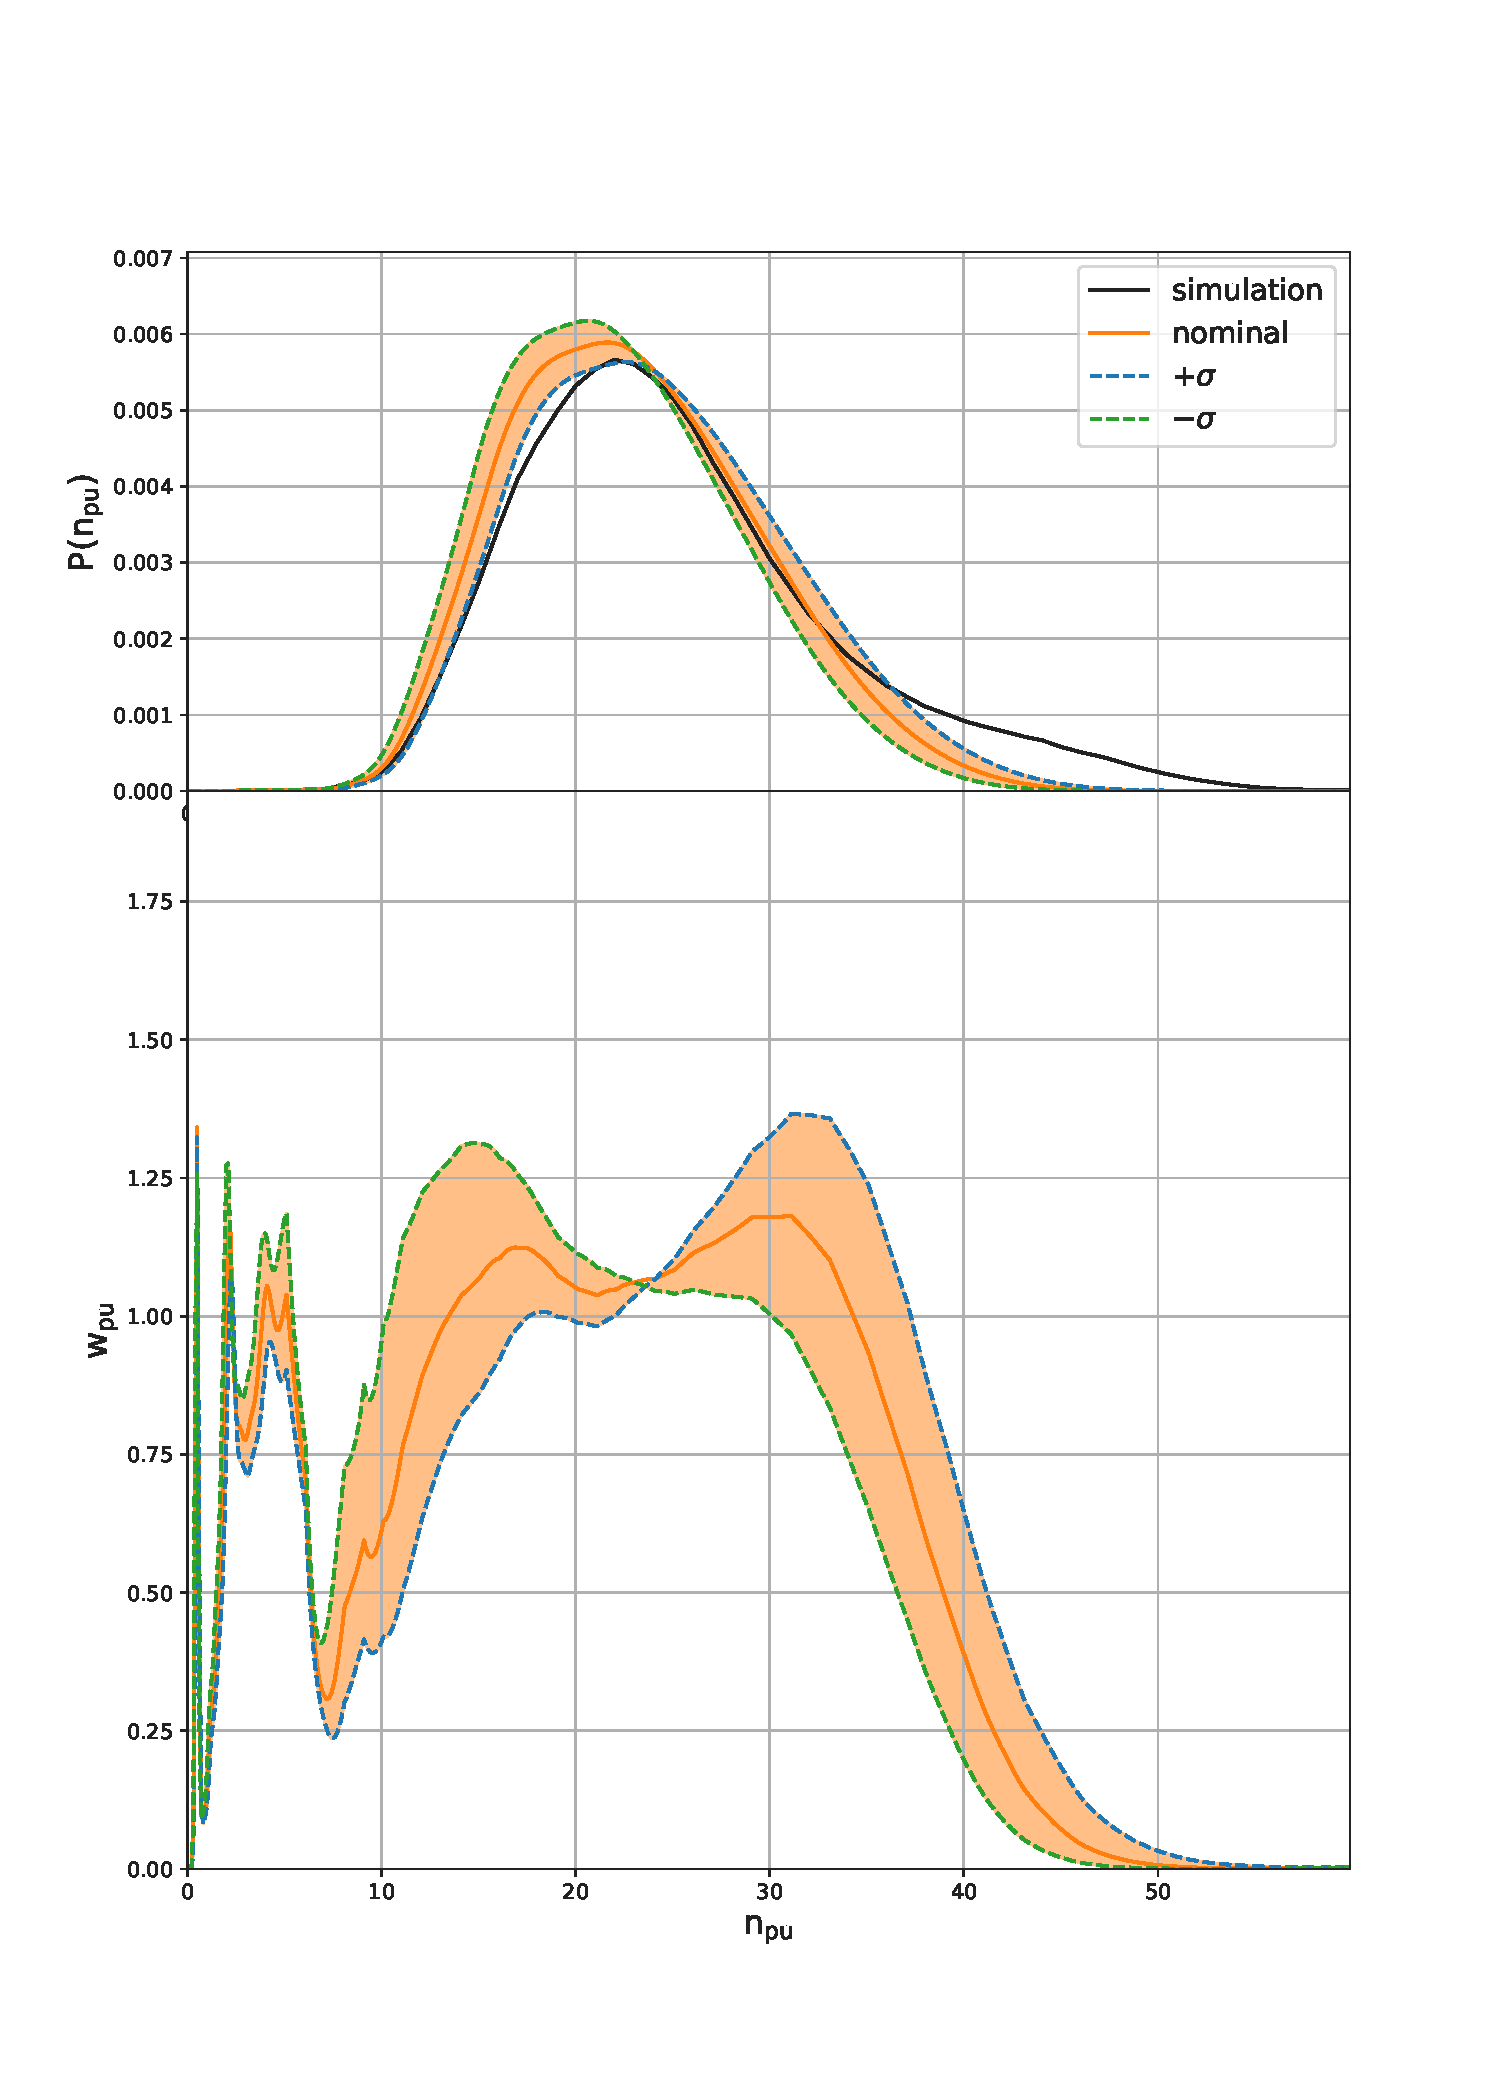
\includegraphics[width=0.35\textwidth]{chapters/Analysis/sectionDataset/figures/pileup_systematics.pdf}
    \caption{(\emph{top}) Pileup distribution in data and simulation including the $\pm\sigma$ variation of the data pileup distributions. (\emph{bottom}) The weights parameterized by number of simulated pileup resulting from taking the ratio of the pileup distribution in data and simulation.}
    \label{fig:analysis:dataset:pileup}
\end{figure}

\begin{figure}[ht]
    \centering
    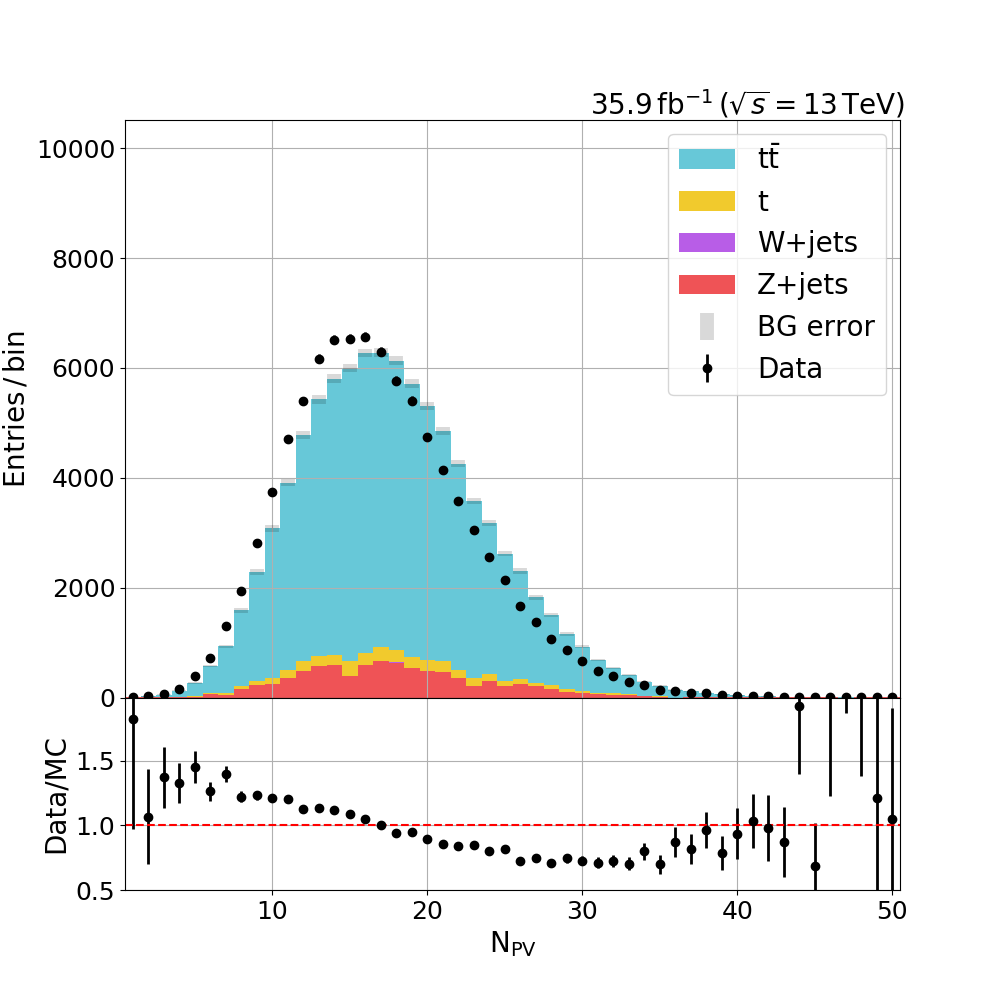
\includegraphics[width=0.45\textwidth]{chapters/Analysis/sectionDataset/figures/n_pv}
    \caption{Comparison of primary vertex multiplicity between data and simulated datasets.}
    \label{fig:analysis:dataset:npv}
\end{figure}
\FloatBarrier


%  top pt
\subsubsection{\cPqt \pt Reweighting}

Additional corrections can be applied to the \ttbar sample to account for generator level mismodeling of the top quark \pt spectrum~\cite{CMS-PAS-TOP-16-011, CMS-PAS-TOP-16-008}.  This is done by identifying the parton-level top quarks, and calculating a scale factor from the equation,

\begin{equation}
    \nonumber
    SF_{t}(\pt) = SF_{\bar{t}}(\pt) = e^{0.0615-0.0005 \pt}.
\end{equation}


The overall event weight is that is applied is $w = \sqrt{SF_{t}SF_{\bar{t}}}$.  For this analysis, we do not apply the weight, but instead include the affect of applying the weight to generate a one-sided morphing template used in the branching fraction determination.  In this case, the nominal value corresponds to the central value of a one-sided Gaussian constraint and the weighted value corresponds to the one-sigma variation up.

\begin{figure}[ht]
    \centering
    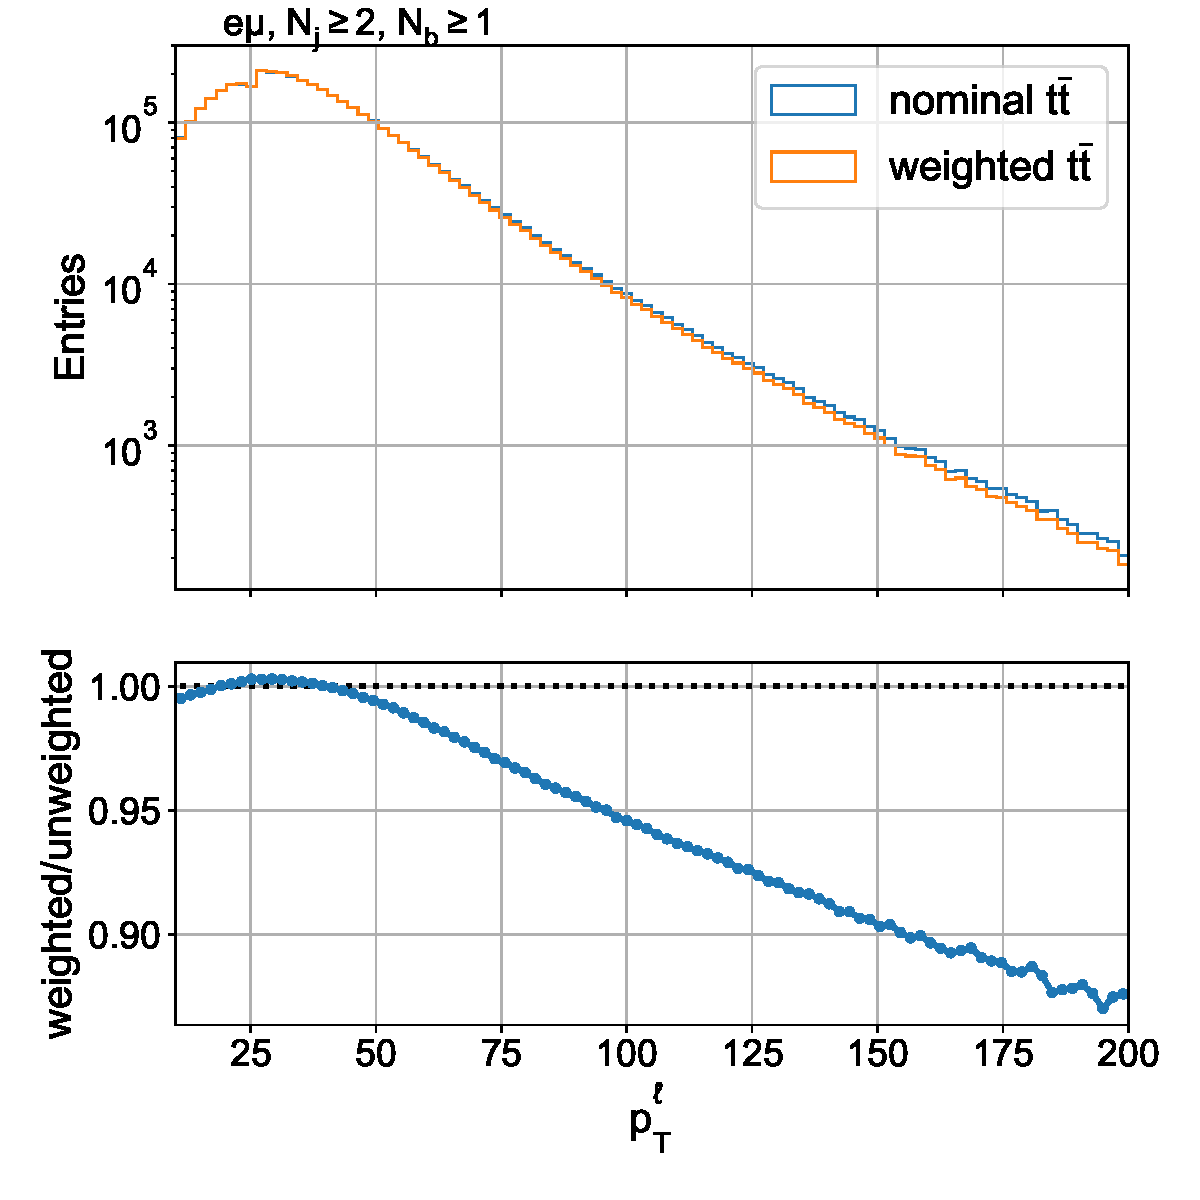
\includegraphics[width=0.55\textwidth]{chapters/Analysis/sectionDataset/figures/top_pt_weight}
    \caption{Comparison of the trailing lepton $\pt$ distribution in $e\mu$ events with at least two jets and at least one b tag with top $\pt$ weights applied and without the weights.}
    \label{fig:analysis:dataset:top_pt_weight}
\end{figure}
\FloatBarrier

% ww pt
\subsubsection{WW \pt Reweighting}
Estimation of the $WW$ process relies on the \POWHEG MC generator which is a NLO fixed order generator. Higher order corrections are therefore not directly included, but have been calculated separately~\cite{Meade:2014fca, Jaiswal:2014yba, Grazzini:2015wpa}.  The estimation of uncertainty is based on the description in section 6 of AN-2017-273. As mentioned there, the theoretical uncertainty associated with the corrections have not been provided so they are estimated by varying the renormalization, factorization, and the matching scale of the \pt resummation technique. The weights and their systematic variations, as well as the effect on the lepton \pt spectrum in the WW MC sample is shown in figure~\ref{fig:analysis:dataset:ww_weight}.

\begin{figure}[ht]
    \centering
    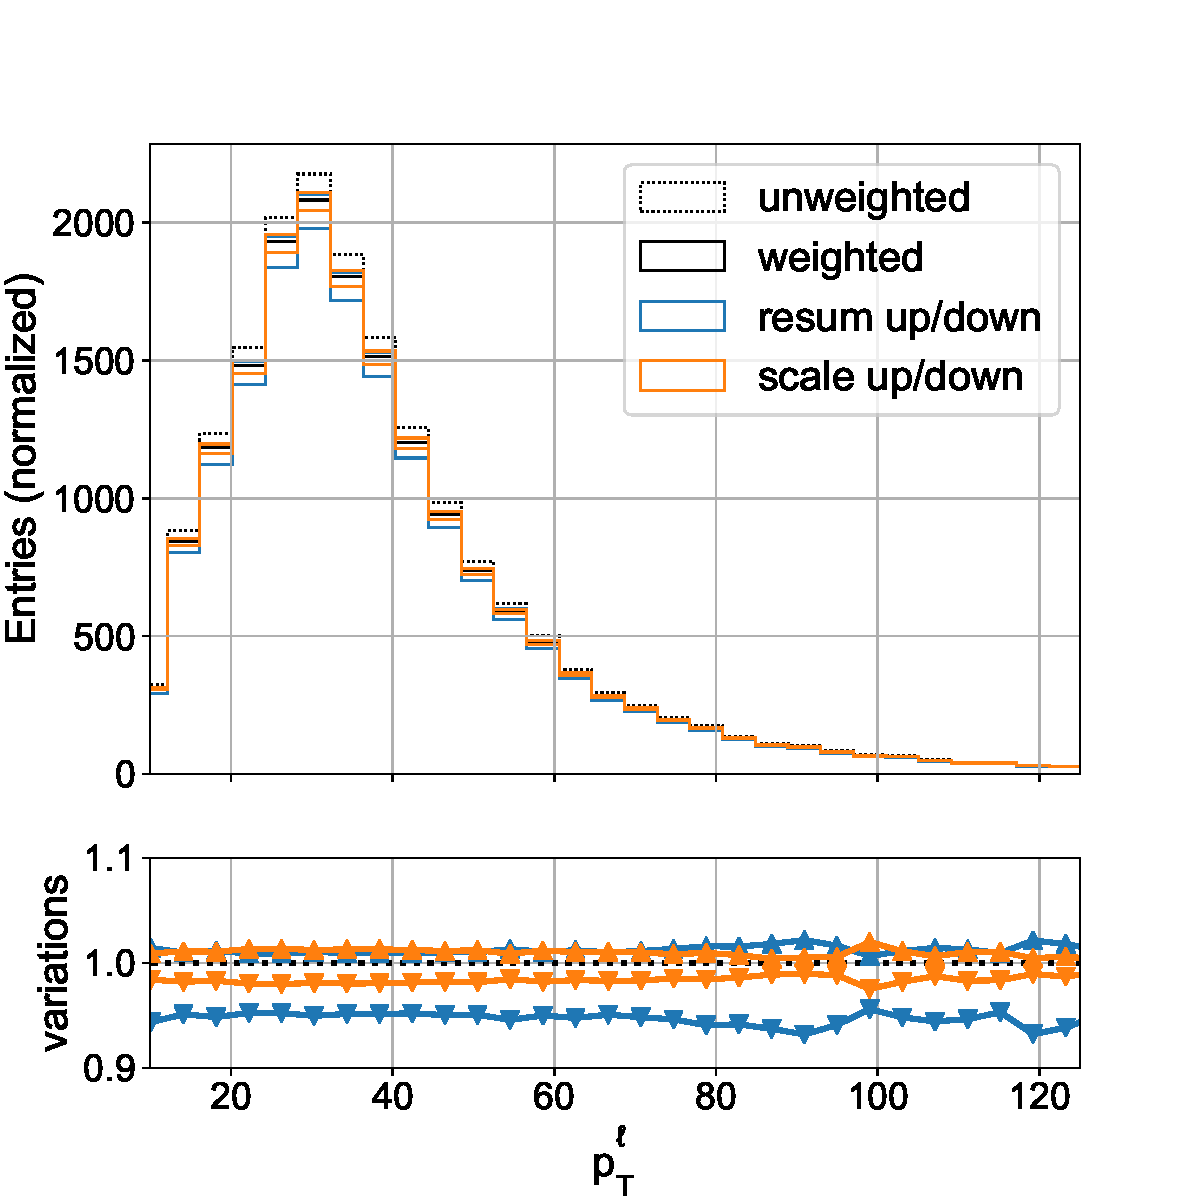
\includegraphics[width=0.45\textwidth]{chapters/Analysis/sectionDataset/figures/ww_pt_lepton_pt}
    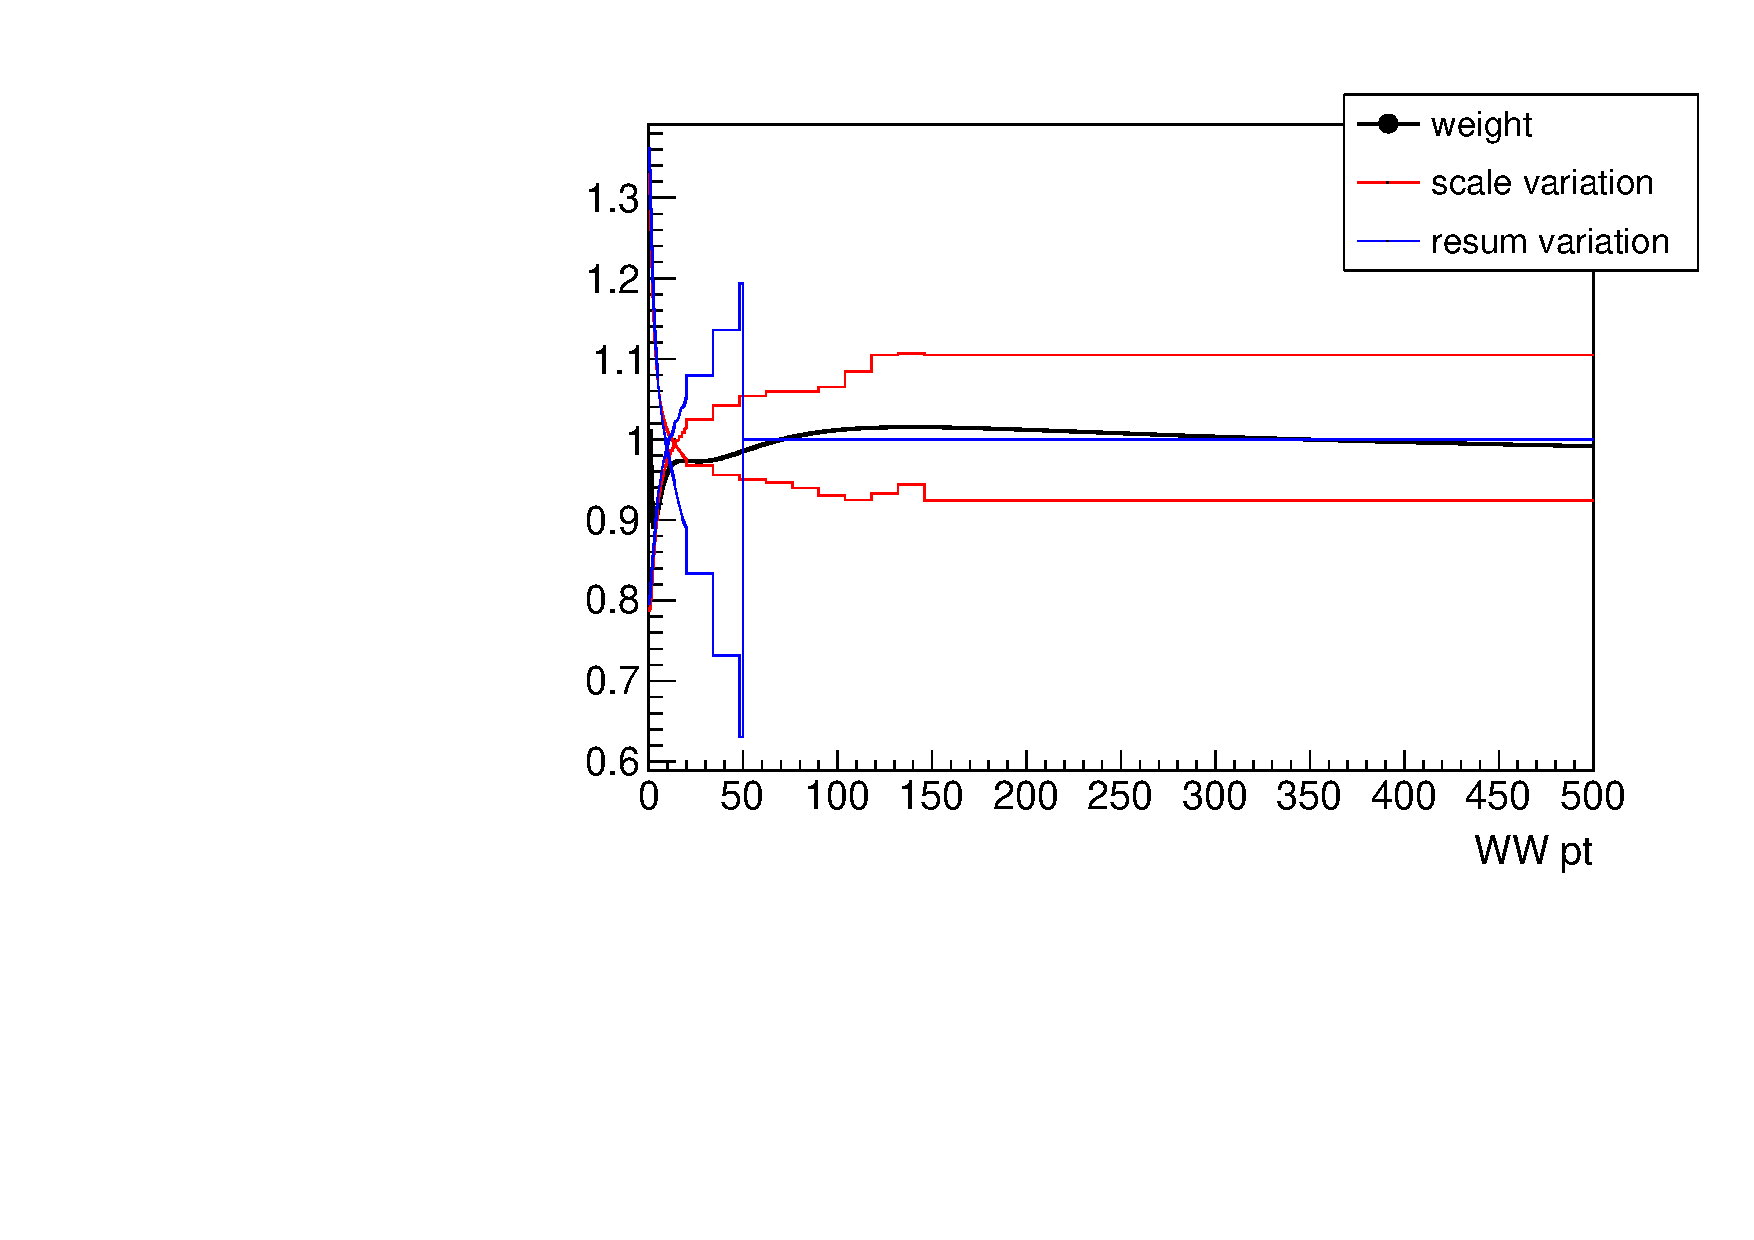
\includegraphics[width=0.45\textwidth]{chapters/Analysis/sectionDataset/figures/ww_pt_weight_variations}
    \caption{\emph{left.} Weights for the $qq\rightarrow WW$ process as a function of the $WW\,\pt$ and the two componnents of systematic variation.  \emph{right.} Trailing lepton pt from the $qq\rightarrow WW\rightarrow e\mu\nu\nu$ simulated sample when there are no reconstructed jets.} 
    \label{fig:analysis:dataset:ww_weight}
\end{figure}

\FloatBarrier


% z pt
\subsubsection{\cPZ \pt Reweighting}
Based on differences between the observed and predicted \PZ \pt spectrums, weights are derived to correct the \pt spectrum in simulation.The derivation of the weights was done in the context of the $H\rightarrow WW$ analysis and is described in AN-2017-082. This correction does not have an associated uncertainty included in the fit.

\begin{figure}[ht]
    \centering
    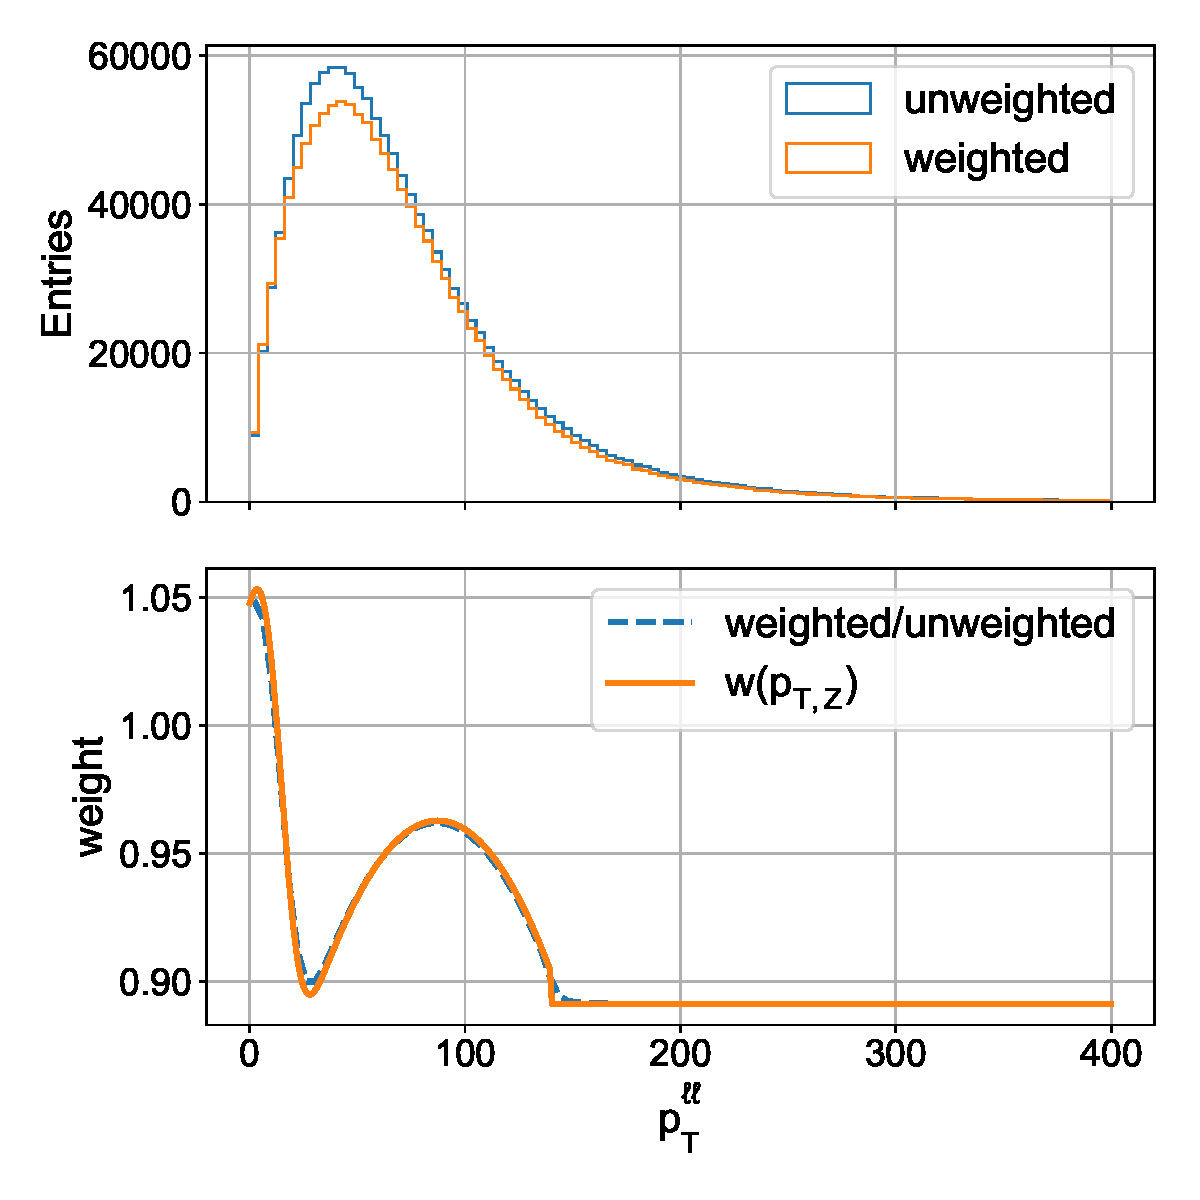
\includegraphics[width=0.45\textwidth]{chapters/Analysis/sectionDataset/figures/z_pt_weighting}
    \caption{\emph{top.} Comparison of weighted and unweighted dilepton \pt spectrum for dimuon events with two jets and no b tags. \emph{bottom.} Comparison between ration of distributions in the top distribution and the analytical function for generating weights.}
    \label{fig:analysis:dataset:ww_weight}
\end{figure}
\FloatBarrier



\section{Selection}
\label{sec:analysis:selection}



\subsection{Object Selection}
The event topologies of interest will require reconstructing electrons, muons, hadronically decaying tau leptons, hadronic jets, and missing tansverse energy (MET).  In this section, the reconstruction and selection of these physics objects is described.



\subsubsection{Primary vertex}
Primary vertices (PV) are reconstructed based on information from the tracking subsystem, mainly through the inner pixel detector. Quality cuts are applied to reconstructed PVs to guarantee they come from a proton-proton hard scattering event. These cuts are as follows,
\begin{equation*}
    N_{\rm d.o.f.}> 4; \quad  \left|z\right| < 24~\mathrm{cm}; \quad \sqrt{x^{2} + y^{2}} < 2~\mathrm{cm}.
\end{equation*}


The PVs are ordered based on the sum \pt of tracks used in their reconstruction. Selected physics objects are associated to the PV with the greatest sum \pt. 




\subsubsection{Muon}
Muon candidates are reconstructed using both the muon and tracker systems. The coverage of these two detector systems allows reconstruction of muons within $\left|\eta\right| < 2.4$ and $p_{T}$ as low as 5 GeV~\cite{Chatrchyan:2012xi}. Muons are required to be reconstructed using both the \emph{global muon} and \emph{tracker muon} reconstruction algorithms. These algorithms are distinct in that one begins with tracker information and extrapolates to find consistency with hits in the muons system (\emph{tracker muons}), while the other (\emph{global muon}) inverts the reconstruction steps starting from the muon system and finding tracks that are consistent. The combination of these two algorithms makes for a muon reconstruction that is accurate in predicting muon momentum and efficient in detecting muons within the detector acceptance.

In the interest of detecting muons decaying from vector bosons, a set of identification and isolation requirements are applied~\cite{Sirunyan:2018fpa}. The muon identification requirements are designed to have high selection efficiency and a low probability of misidentifying non-prompt muons originating from non-bosonic decays. The muon POG provided selection criteria are listed in table~\ref{tab:muon_id}.

\begin{table}[ht]
    \centering
    \setlength{\tabcolsep}{2em}
    \renewcommand{\arraystretch}{1.25}
    % \small
    \caption{Tight muon identification criteria as provided by muon POG}
    \label{tab:muon_id}
    \begin{tabular}{l|c}
    variable                            & cut value \\
    \hline
    isGlobal                            & True      \\
    isPF                                & True      \\
    $\chi^{2}$                          & $< 10$    \\
    number of matched stations          & $> 1$     \\
    number of pixel hits                & $> 0$     \\
    number of track layers              & $> 5$     \\
    number of valid hits                & $> 0$     \\
    $|d_{xy}|$                          & $< 0.2$   \\
    $|d_{z}|$                           & $< 0.5$    \\
    \hline
    $ISO_{PF}/p_{T}$ ($\rho$ corrected) & $< 0.15$
    \end{tabular}
\end{table}


\noindent To increase the likelihood of selecting muons produced by the prompt decay of vector bosons, an isolation requirement is placed on all muons. The isolation of the muon is calculated by summing the \pt of all charged hadronic, neutral hadronic, and photon particle flow candidates in a cone of radius $\Delta R = 0.4$ about the muon candidate. This quantity is corrected to remove the contamination of the neutral component due to pileup by subtracting off the average energy deposited by pileup. It is defined as,
\begin{equation}
    I_{\rm PF} = I_{\rm ch. had} + \max \left(0, I_{\rm neu. had} +
    I_{\gamma} - 0.5 I_{\rm PU}\right)
\end{equation}

Simulated events are reweighted to account for differences in the muon reconstruction, identification, and isolation efficiencies with respect to data.







\subsubsection{Electron}

Electrons are reconstructed by combining information from the electromagnetic calorimeter and the tracking system using a gaussian-sum
filter (GSF) method \cite{Baffioni:2006cd}.  Corrections are applied to account for mismeasurement of electron momentum scale and resolution. All electrons are required to have $\pt \geq 20~\GeV$ and $|\eta| < 2.5$.  Electrons are identified using a tight cut-based scheme. The requirements for this selection are listed in table~\ref{tab:slt:electron_id}.

\begin{table}[ht]
    \centering
    \setlength{\tabcolsep}{2em}
    \renewcommand{\arraystretch}{1.25}
    % \small
    \caption{Tight electron identification criteria as provided by the egamma POG.}
    \label{tab:slt:electron_id}

    \begin{tabular}{l|c|c}
        variable                          & $|\eta| < 1.4446$ & $|\eta| \geq 1.566$ \\
        \hline
        $\sigma_{i\eta}\sigma_{i\eta}$    & $<0.00998$        & $0.0394$            \\
        $|d\eta|$                         & $<0.00308$        & $0.0292$            \\
        $|d\phi|$                         & $<0.0816$         & $0.00605$           \\
        $H/E$                             & $<0.0414$         & $0.0641$            \\
        $|\frac{1}{E} - \frac{1}{p}|$     & $<0.0129$         & $0.0129$            \\
        missing hits                      & $\leq 1$          & $\leq 1$            \\
        $|d_{0}|$                         & $<1.$             & $<1.$               \\
        \hline
        conversion rejection              & true              & true                \\
        ISO$_{PF}$/$p_{T}$ (EA corrected) & $< 0.0588$        & $<0.0571$           \\
    \end{tabular}
\end{table}

\noindent The electrons are also required to pass a tight isolation criteria. The isolation variable is constructed by summing the energy of charged and neutral particle flow objects within a cone of radius $\Delta R = 0.4$ about the electron candidate and subtracting off the contribution from pileup.  The combined particle flow isolation with the pileup correction is,
\begin{equation}
    \nonumber
    I_{\rm comb} = I_{\rm ch. had.} + \max\left(  0, I_{\rm neu. had.} + I_{\gamma} - \rho EA(|\eta_{e}|) \right).
\end{equation}

The pileup correction is dependent on the parameter $\rho$ which correlates with the average energy due to pileup, and the effective area which changes depending on the $|\eta|$ value of the electron.





\subsubsection{Hadronic Tau}

Hadronically decaying $\tau$ leptons are reconstructed using the hadron-plus-strips algorithm~\cite{ref:cms-tau}. This algorithm constructs candidates seeded by a PF jet that are consistent with either a single or triple charged pion decay of the $\tau$ lepton.  In the single charged pion decay mode, the presence of neutral pions is detected by reconstructing their photonic decays. If the hadronic tau candidate is found to overlap ($\Delta R < 0.3$) with either an electron or muon passing the analysis selections listed above, the tau candidate is rejected. Jets originating from non-$\tau$ decays are rejected with a MVA discriminator that takes into account the pileup contribution to the neutral component of the $\tau$ decay~\cite{CMS-TAU-16-003-001}.  

Reconstructed hadronic taus are required to have $p_{T} > 20$ GeV and $|\eta| < 2.3$ unless noted otherwise.  It is observed that the counting analysis is more sensitive to misidentification of hadronic jets as hadronic tau candidates, so while the tight working point is used in the shape analysis, the very tight working point is used for the counting analysis.

The scale factor accounting for different tau reconstruction and identification efficiencies were measured in several control regions~\cite{CMS-TAU-16-003-001}.  The measurement is carried out in both in two different control regions: one enriched in $Z\to\tau\tau$ production and one enriched in \ttbar.  Because of the large overlap with our signal region in the case of the latter, the former measurement is used so that the datasets that are used are uncorrelated.  For the selection algorithm and tight working point a scale factor of $0.95 \pm 0.05$ is used; for the very tight working point it is $0.92 \pm 0.05$.






\subsubsection{Jet}
Jets are reconstructed from PF candidates \cite{ref:pf}. PF candidates combine information from all of the detector subsystems to facilitate the reconstruction and identification of individual particles.  These PF candidates are clustered using the anti-$k_{t}$ algorigthm \cite{Cacciari:2008gp} with a cone size of $\Delta R = 0.4$. Once reconstructed, a number of corrections are applied to the jets to correct for pileup contamination, differing absolute response in jet \pt, and relative response in $\eta$ \cite{ref:jetscale}.  To reduce contamination from photons and prompt leptons, several ID requirements are placed on the jets and are listed in table~\ref{tab:slt:jet_id_2016}.

\begin{table}[ht]
    \centering
    \setlength{\tabcolsep}{0.8em}
    \renewcommand{\arraystretch}{1.25}
    % \small
    \caption{Jet ID requirements for 2016.}
    \label{tab:slt:jet_id_2016}
    \begin{tabular}{l|ccc}
        \hline
                                    & $|\eta| < 2.4$ & $2.4 < |\eta| \leq 3.0$ & $3.0 < |\eta| \leq 4.7$ \\
        \hline                                                                   
        number of constituents         & $> 1$          & $> 1$                  & -- \\
        neutral hadronic fraction      & $< 0.99$       & $< 0.99$               & -- \\
        neutral EM fraction            & $< 0.99$       & $< 0.99$               & $<0.9$ \\
        charged hadronic fraction      & $> 0$          & --                     & -- \\
        charged EM fraction            & $< 0.99$       & --                     & -- \\
        number of charged constituents & $> 0$          & --                     & -- \\
        number of neutrals             & --             & --                     & $>10$                   \\
        \hline
    \end{tabular}
\end{table}

\noindent In addition to the above requirements, it is required that all jets have $\pt > 30$ GeV and $\left|\eta\right| < 4.7$.  Jets are vetoed if they overlap with a muon, electron, or tau passing the identification requirements described above within a cone size of $\Delta R = 0.3$. 

\subsubsection{b-Tag} The identification of jets originating from the decay of b quarks is done using the CSV b-tagging algorithm~\cite{Sirunyan:2298594} is used to optimize the efficiency for identifying b-jets while reducing the misidentification from jets originating from light quark (usdg).  In this analysis, the recommended medium working point ($\text{CSV} > 0.8484$) supplied by the b tag POG is used.  

To account for the difference in b tag efficiency in data and simulation, the b tag status of jets is modified based on a set of scale factors derived by the b tag POG.  The method used for applying the b tag scale factors modifies the status of individual jets to either promote or demote their b tagging status~\cite{twiki:btag_method}.  The method relies on the user measuring the b tag and mistag efficiencies in the simulated samples.  This is described further in Section~\label{sec:app:btag}.


\FloatBarrier

% ===========================
% Event Selection
% ===========================
\subsection{Event Selection}

The event selection begins by requiring an event pass the lowest \pt theshold single electron or muon trigger that is not prescaled. From these datasets it is possible to select on a number of $\PW\PW$-like final states originating from \ttbar and tW production.  These final states are constructed based on the number of reconstructed leptons, jet multiplicity, and b tag multiplicity.  The categorization of these events differs between the counting and shape analysis.  The common definition of the categories are listed below.


\begin{itemize}
    \singlespacing
    \item $ee$:
    \begin{itemize}
        \item exactly two electrons
        \item $p_{T} > 30, 20$ GeV
        \item reject events with hadronic taus or muons
        \item Z boson veto ($N_{b} \geq 1$ only): $M_{ee} < 75$ or $M_{ee} > 105\,\GeV$
    \end{itemize}
    \item $\mu\mu$:
    \begin{itemize}
        \item exactly two muons
        \item $p_{T} > 25, 10$ GeV
        \item reject events with hadronic taus or electrons
        \item Z boson veto ($N_{b} \geq 1$ only): $M_{\mu\mu} < 75$ or $M_{\mu\mu} > 105\,\GeV$
    \end{itemize}
    \item $e\mu$:
    \begin{itemize}
        \item exactly one electron and one muon
        \item lead muon (electron) $p_{T} > 25 (30)\,\GeV$
        \item trailing muon (electron) $p_{T} > 10\,(20)\,\GeV$
        \item reject events with hadronic taus 
        \item events in electron datastream that fire muon trigger are vetoed
    \end{itemize}
    \item $e\tau$:
    \begin{itemize}
        \item exactly one electron and one hadronic tau
        \item $p_{T} > 30, 20$ GeV
        \item reject events with muons
    \end{itemize}
    \item $\mu\tau$:
    \begin{itemize}
        \item exactly one muon and one hadronic tau
        \item $p_{T} > 25, 20$ GeV
        \item reject events with electrons
    \end{itemize}
    \item e + jets:
    \begin{itemize}
        \item exactly one electron 
        \item $p_{T} > 30$ GeV
        \item reject events with muons or hadronic taus
        \item at least four jets
    \end{itemize}
    \item $\mu + jets$:
    \begin{itemize}
        \item exactly one muon 
        \item $p_{T} > 25$ GeV
        \item reject events with electrons or hadronic taus
        \item at least four jets
    \end{itemize}
\end{itemize}




These selections are designed to primarily target $\ttbar$ production and specific \PW decay modes. The final states will tend to only contain events from a single datastream except for the $e\mu$ selection which has non-negligible overlap between the electron and muon datastreams. Any overlap in events between the two datastreams are removed by only taking the event from single muon datastream. Because the tau can decay to an electron, muon, or hadronically, each of these channels has some mixing between terms arising from $W\rightarrow\ell$ decays and $W\rightarrow\tau\rightarrow\ell$ decays.  The mixing between the selected final states and the underlying W boson decays are shown in table~\ref{tab:signal_breakdown}. These numbers are estimated from simulated \ttbar events and are consequently dependent on the values of branching fractions used in the simulation.  

For the counting analysis, there is always a requirement that there be at least two jets and at least one b tagged jet. The categories are partitioned based on whether there is exactly one b jet or there are two or more b jets.  Additionally, the $e\mu$ selection is split into muon triggered and electron triggered categories: if the muon has the highest \pt and the muon trigger has fired it categorized as a $\mu e$ event; if the electron has highest \pt and the electron trigger fired it is categorized as an $e \mu$ event.

The shape analysis takes advantage of subdividing the data into several additional b tag and jet multiplicity categories to constrain systematics uncertainties, and to take advantage of higher tau reconsruction purity in lower jet multiplicity bins.  The categories are shown in table~\ref{tab:jet_categories}.  As described in the list above, the $ee$ and $\mu\mu$ categories have a Z veto applied in the case that there are one or more b tags; this requirement is not applied in the zero b tag case.  There is also a set of requirements to enhance the proportion of Drell-Yan in the $e\tau$ and $\mu\tau$ categories in the case that the number of jets is 0 or 1 and there are no b tags.  The requirements are constructed to mainly reduce the W boson contribution and are :
\begin{equation*}
    40 \GeV \leq M_{\ell\tau_{h}} \leq 100 \GeV, \quad
    \Delta\phi(\ell, \tau_{h}) > 2.5, \quad
    M_{T}^{\ell} < 60 \GeV,
\end{equation*}

\noindent where $M_{T}^{\ell}$ is the transverse mass of the electron or muon,
\begin{equation}
\label{eq:trans_mass}
    M_{T,\ell} = \sqrt{2 p_{T}^{\ell}\MET (1-\cos\Delta\phi(p_{T}^{\ell}, \MET))}.
\end{equation}


\begin{table}[]
    \centering
    \setlength{\tabcolsep}{1.5em}
    \renewcommand{\arraystretch}{1.1}
    \caption{Categories used in the shape analysis based on jet and b
    tag multiplicities.}
    
    \begin{tabular}{l|c|c|c|c}
                                    & $N_{j} = 0$        & $N_{j} = 1$        & $N_{j} = 2$        & $N_{j} \geq 3$     \\
	\hline
    \multirow{2}{*}{$N_{b} = 0$}    & $e\tau$, $\mu\tau$ & $e\tau$, $\mu\tau$ & \multicolumn{2}{c}{$e\tau$, $\mu\tau$} \\
                                    & $e\mu$             & $e\mu$             & \multicolumn{2}{c}{$ee, \mu\mu, e\mu$} \\
	\hline
    \multirow{3}{*}{$N_{b} = 1$}    &                    & $e\tau$, $\mu\tau$ & $e\tau$, $\mu\tau$ & $e\tau$, $\mu\tau$ \\
	\cline{4-5}
                                    &                    & $e\mu$             & \multicolumn{2}{c}{$ee, \mu\mu, e\mu$}  \\
                                    &                    &                    & \multicolumn{2}{c}{$ej$, $\mu j$}  \\
	\hline
    \multirow{3}{*}{$N_{b} \geq 2$} & \multicolumn{2}{c|}{}                   & $e\tau$, $\mu\tau$ & $e\tau$, $\mu\tau$ \\
	\cline{4-5}
                                    & \multicolumn{2}{c|}{}                   & \multicolumn{2}{c}{$ee, \mu\mu, e\mu$}  \\
                                    & \multicolumn{2}{c|}{}                   & \multicolumn{2}{c}{$ej$, $\mu j$}  \\
	\hline
    \end{tabular}
    
    \label{tab:jet_categories}
\end{table}


% \begin{table}[ht]
	\centering
	\setlength{\tabcolsep}{0.4em}
    \renewcommand{\arraystretch}{1.5}
    \small
    
    \begin{tabular}{|cc|cc|cc|cc|}
    
    %%%%%%%%%%%%%%%%%%
	% mu-trigger
	%%%%%%%%%%%%%%%%%%
    \multicolumn{8}{c}{single muon trigger} \\
    \hline
    \multicolumn{2}{|c|}{$\mu e$} 					& \multicolumn{2}{c|}{$\mu\mu$} 				  & \multicolumn{2}{c|}{$\mu \tau$} 					& \multicolumn{2}{c|}{$\mu + jets$} 			  	\\
    \hline
    1b & 2b                   						& 1b & 2b        	 						      & 1b & 2b        										& 1b & 2b         			        				\\
    \hline 
    \multicolumn{2}{|c|}{$n_{e,\mu,\tau_h} = 1,1,0$}& \multicolumn{2}{c|}{$n_{e,\mu,\tau_h} = 0,2,0$} & \multicolumn{2}{c|}{$n_{e,\mu,\tau_h} = 0,1,1$}      & \multicolumn{2}{c|}{$n_{e,\mu,\tau_h} = 0,1,0$} 	\\
    \multicolumn{2}{|c|}{$p^T_\mu,p^T_e>25,15$ GeV} & \multicolumn{2}{c|}{$p^T_\mu,p^T_\mu>25,10$ GeV}& \multicolumn{2}{c|}{$p^T_\mu,p^T_{\tau_h}>30,20$ GeV}& \multicolumn{2}{c|}{$p^T_\mu>30$ GeV}           	\\
    \multicolumn{2}{|c|}{$p^T_\mu>p^T_e$} 			& \multicolumn{2}{c|}{$|m_{\mu\mu}-m_Z|>15$ GeV } & \multicolumn{2}{c|}{ --- }						     & \multicolumn{2}{c|}{ --- } 						\\
    \multicolumn{2}{|c|}{$n_{jet}\geq2$}			& \multicolumn{2}{c|}{$n_{jet}\geq2$}             &  \multicolumn{2}{c|}{$n_{jet}\geq2$} 				 & \multicolumn{2}{c|}{$n_{jet}\geq4$}             	\\
    \hline

    
    %\multicolumn{8}{c}{} \\
    \multicolumn{8}{c}{single electron trigger} \\
    
    %%%%%%%%%%%%%%%%%%
	% e-trigger
	%%%%%%%%%%%%%%%%%%
    \hline
    \multicolumn{2}{|c|}{$e e$} 					& \multicolumn{2}{c|}{$e \mu$} 				      & \multicolumn{2}{c|}{$e \tau$} 			     		& \multicolumn{2}{c|}{$e + jets$} 			     	\\
    \hline
    1b & 2b                   						& 1b & 2b        	 						      & 1b & 2b        										& 1b & 2b         			        				\\
    \hline 
    \multicolumn{2}{|c|}{$n_{e,\mu,\tau_h} = 2,0,0$}& \multicolumn{2}{c|}{$n_{e,\mu,\tau_h} = 1,1,0$} & \multicolumn{2}{c|}{$n_{e,\mu,\tau_h} = 1,0,1$}      & \multicolumn{2}{c|}{$n_{e,\mu,\tau_h} = 1,0,0$} 	\\
    \multicolumn{2}{|c|}{$p^T_e,p^T_e>30,15$ GeV}   & \multicolumn{2}{c|}{$p^T_e,p^T_\mu>30,10$ GeV}  & \multicolumn{2}{c|}{$p^T_e,p^T_{\tau_h}>30,20$ GeV}  & \multicolumn{2}{c|}{$p^T_e>30$ GeV}           	\\
    \multicolumn{2}{|c|}{$|m_{ee}-m_Z|>15$ GeV }    & \multicolumn{2}{c|}{$p^T_e>p^T_\mu$}   		  & \multicolumn{2}{c|}{ --- }						     & \multicolumn{2}{c|}{ --- } 						\\
    \multicolumn{2}{|c|}{$n_{jet}\geq2$}			& \multicolumn{2}{c|}{$n_{jet}\geq2$}             & \multicolumn{2}{c|}{$n_{jet}\geq2$} 				 & \multicolumn{2}{c|}{$n_{jet}\geq4$}             	\\
    \hline
    
    \end{tabular}
    
    \caption{Analysis selections of 8 channels based on single muon and single electron triggers.}
    \label{tab:slt:eventSelection}
\end{table}


% \begin{figure}[ht]
%     \centering
%     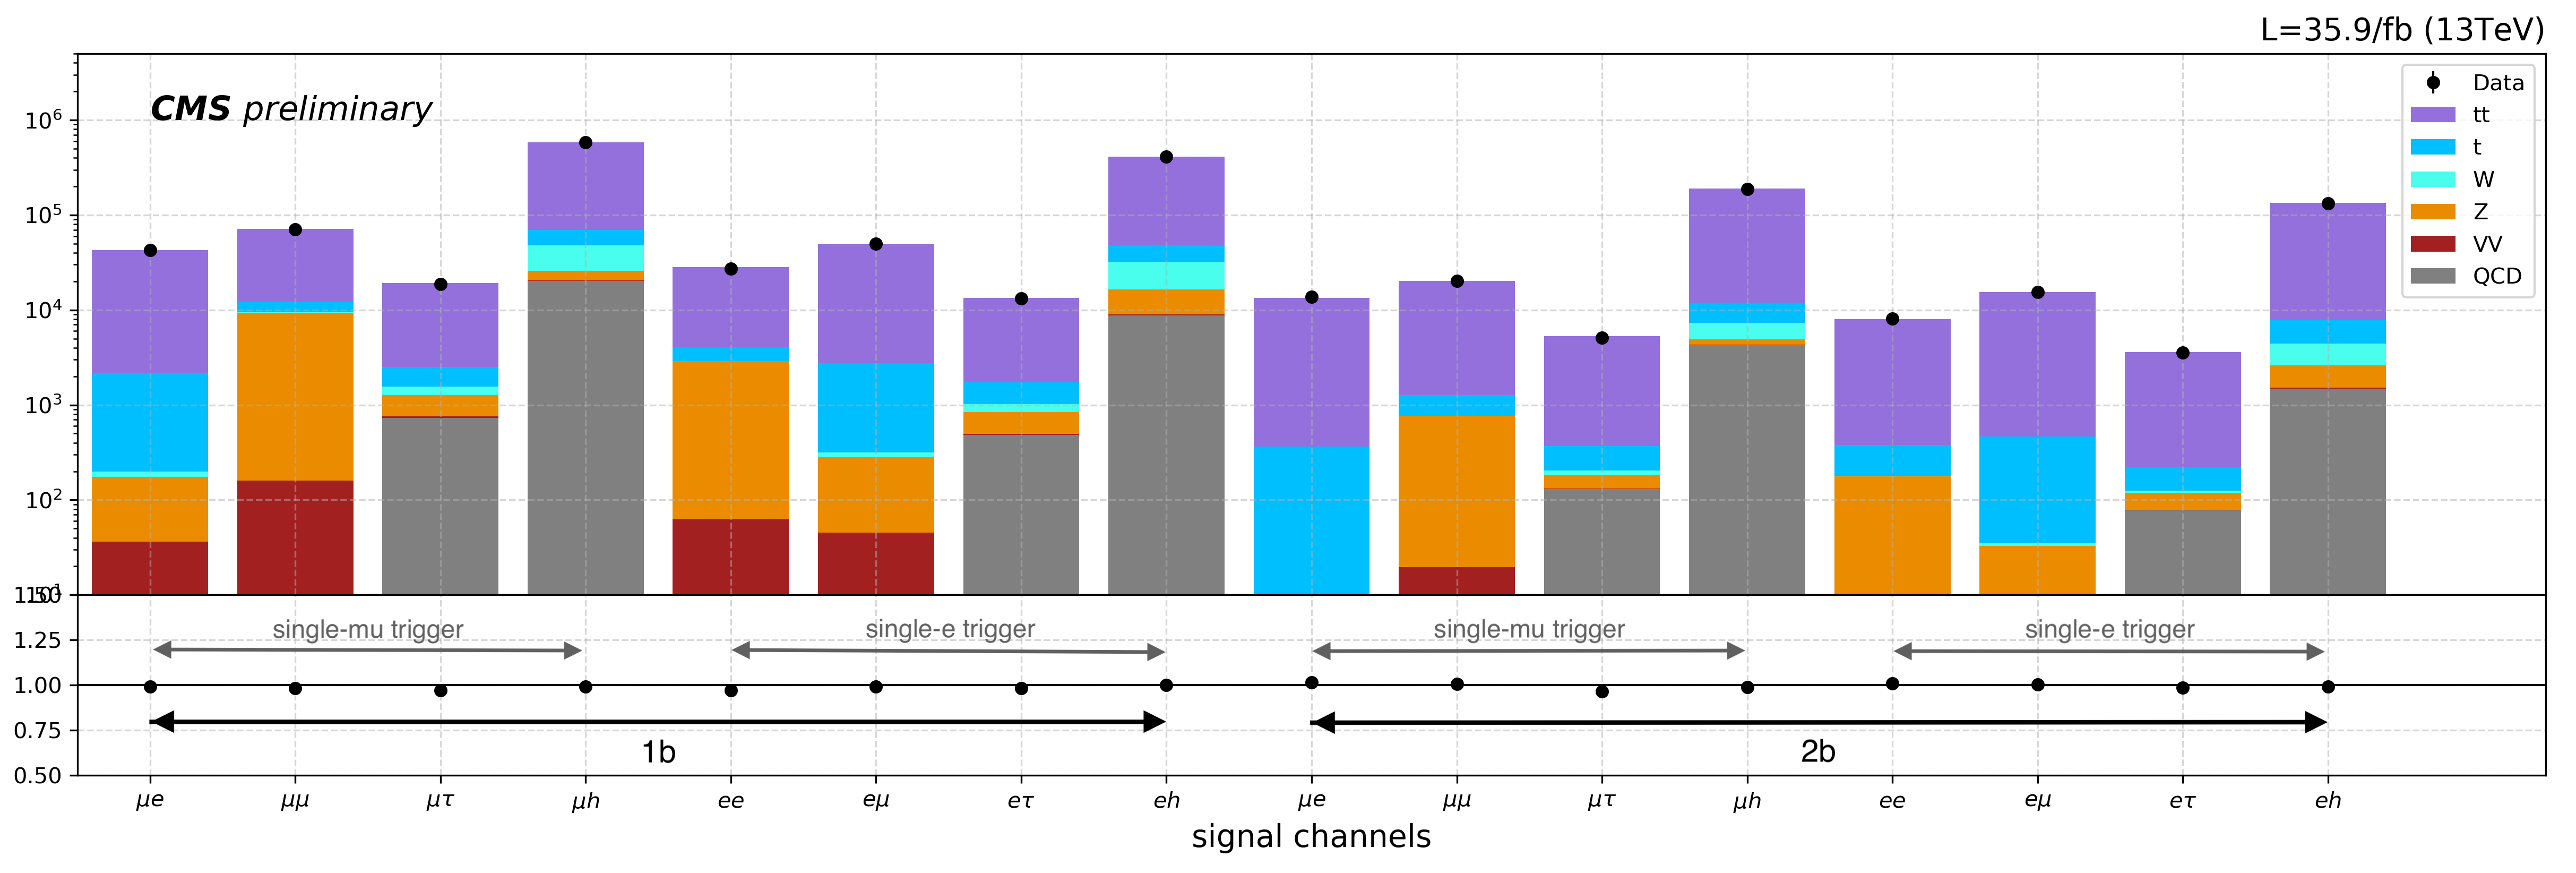
\includegraphics[width=0.99\textwidth]{chapters/Analysis/sectionSelection/figures/counting.png}
%     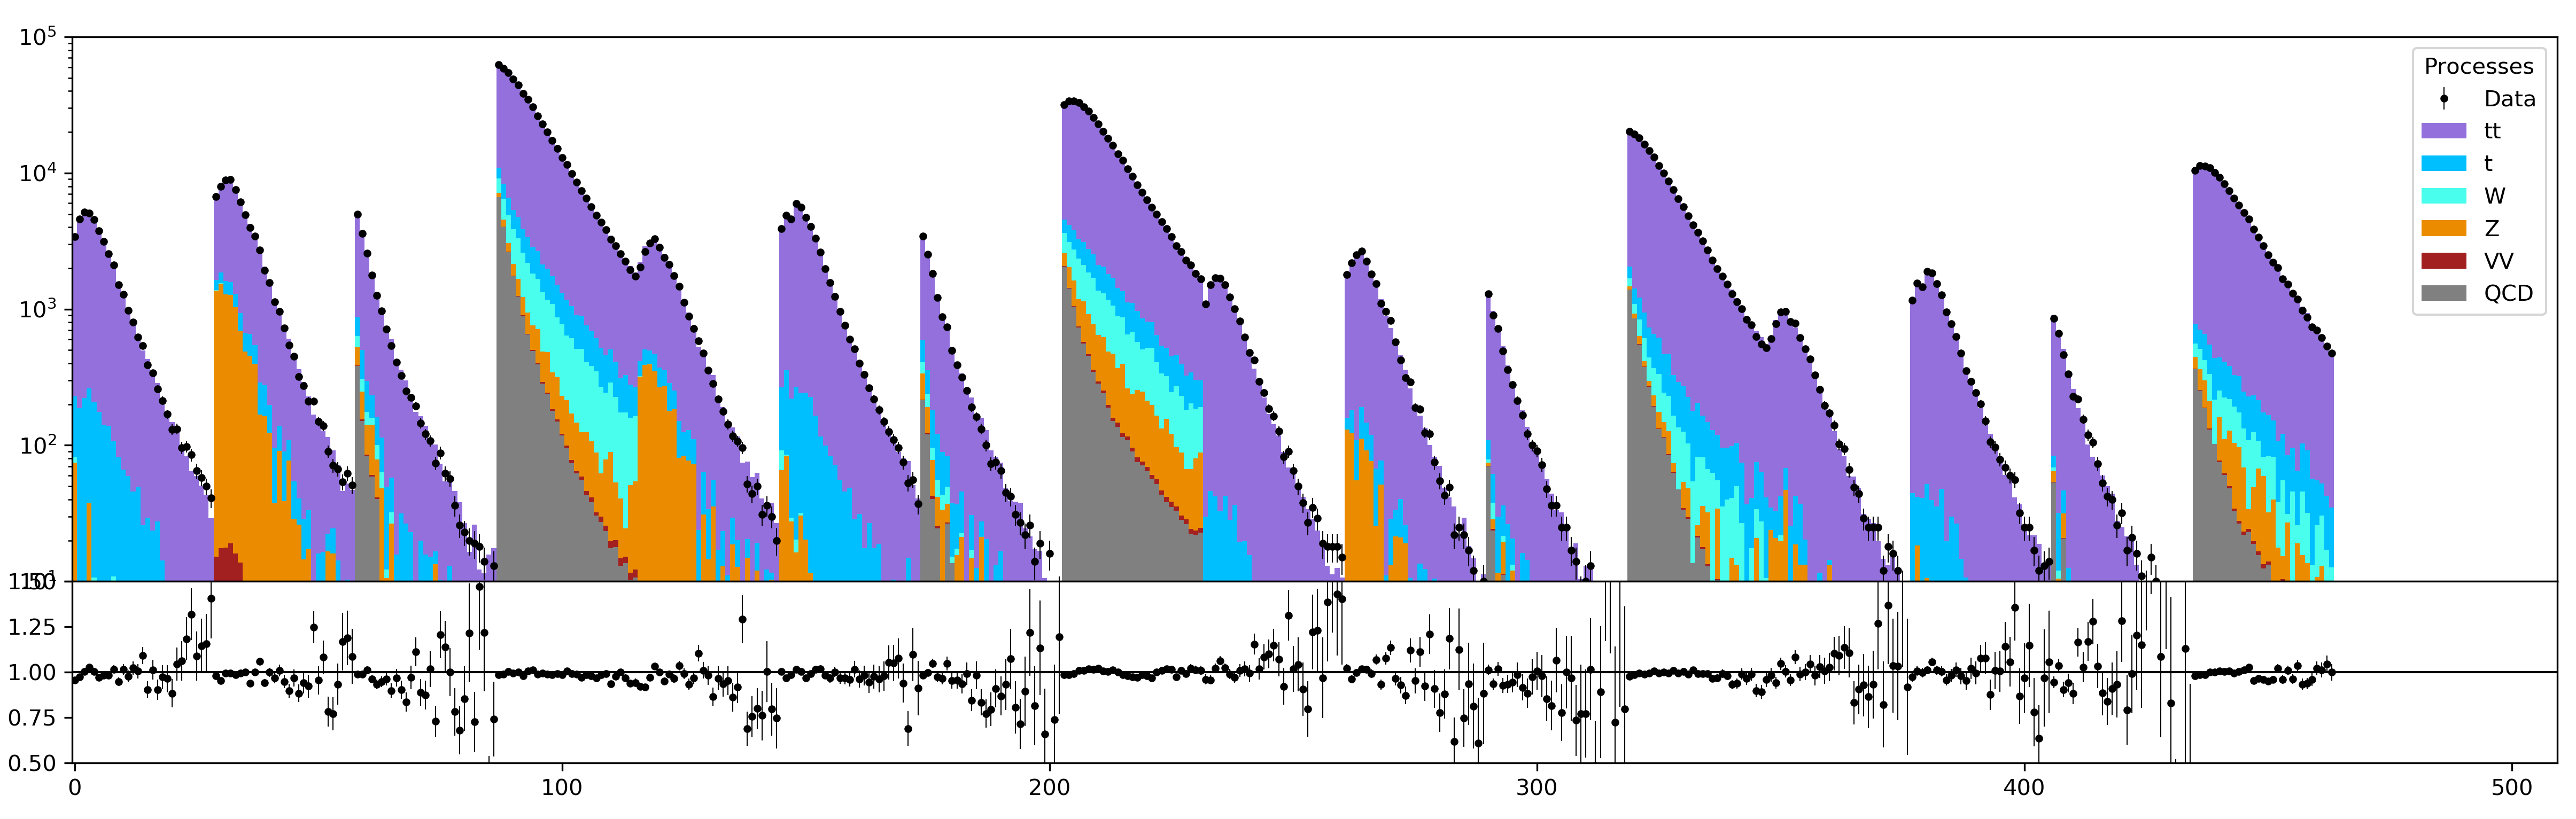
\includegraphics[width=0.99\textwidth]{chapters/Analysis/sectionSelection/figures/shaping.png}
%     \caption{caption}
%     \label{fig:analysis:selection:yields}
% \end{figure}


% \begin{figure}[ht]
%     \centering
%     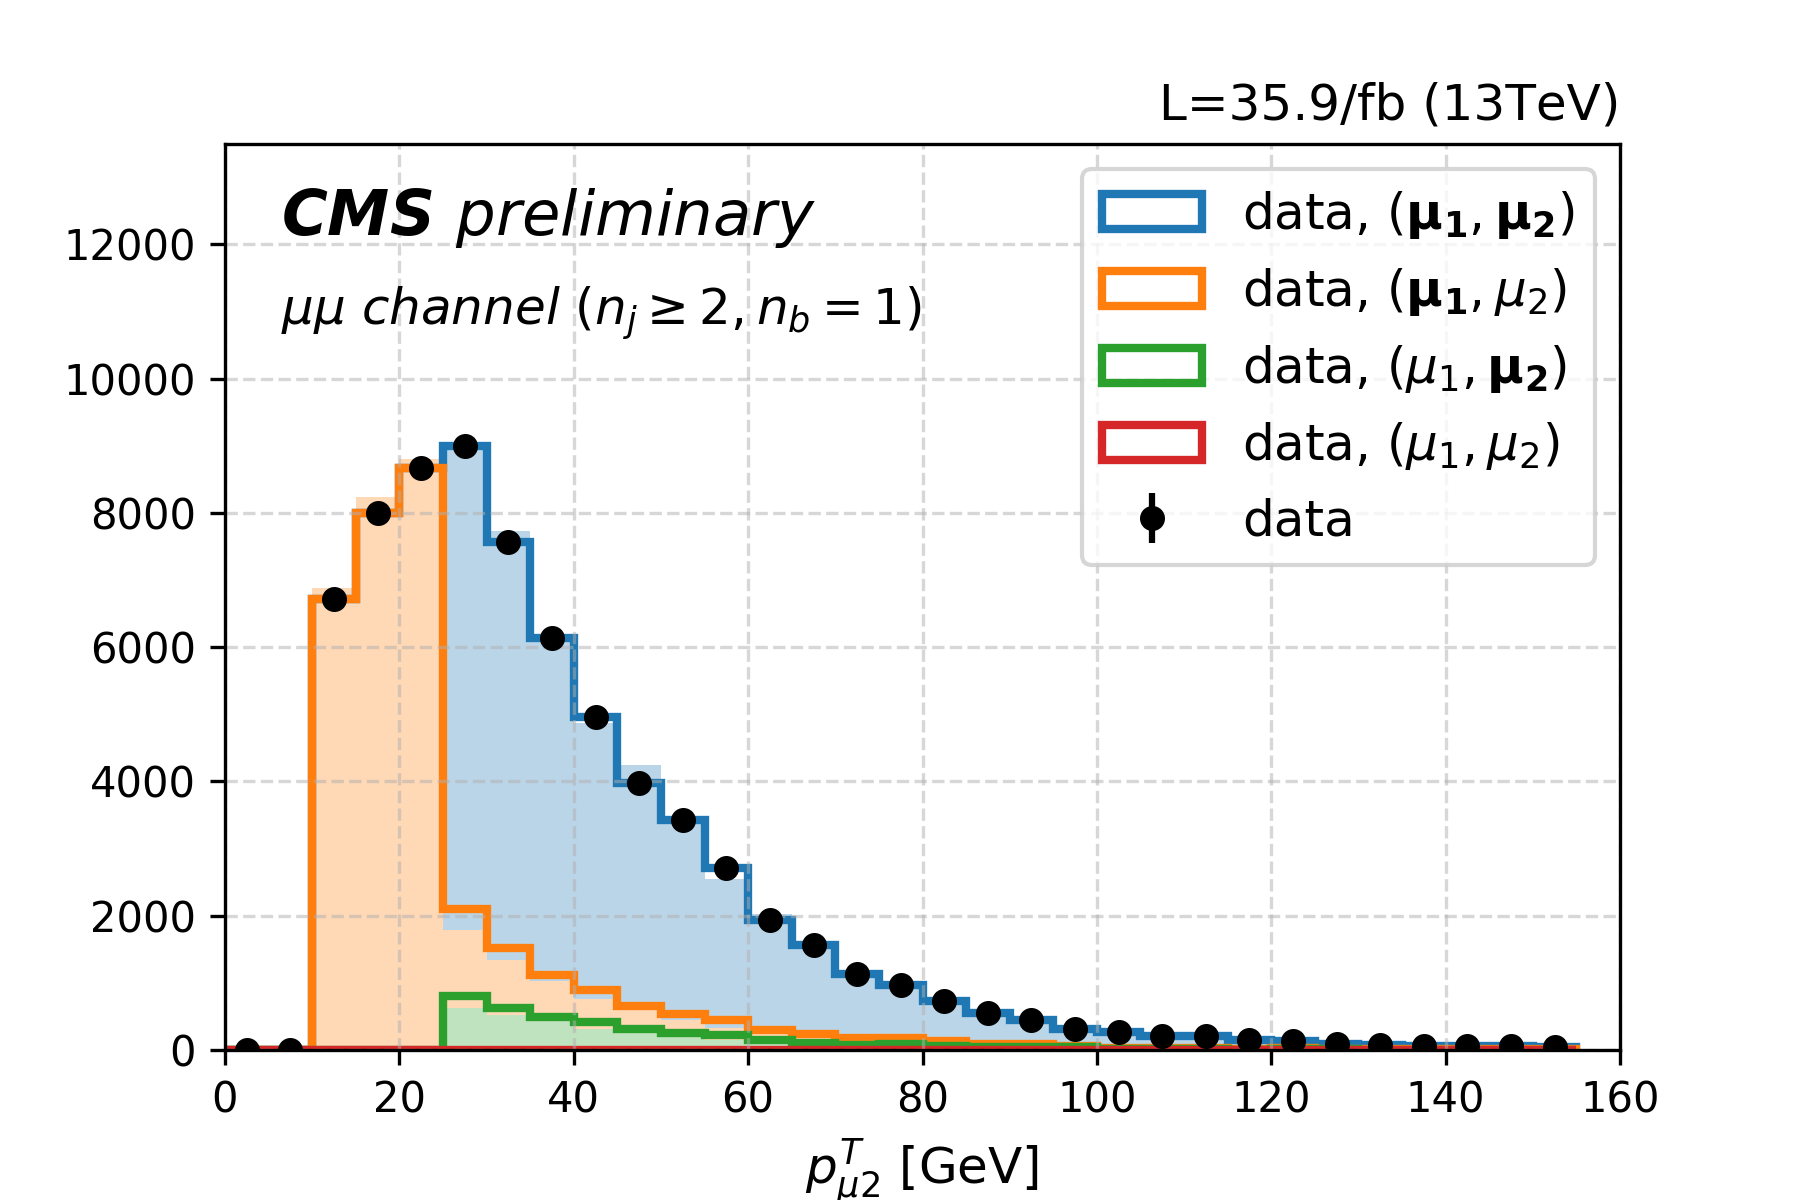
\includegraphics[width=0.49\textwidth]{chapters/Analysis/sectionSelection/figures/trgLep_mumu.png}
%     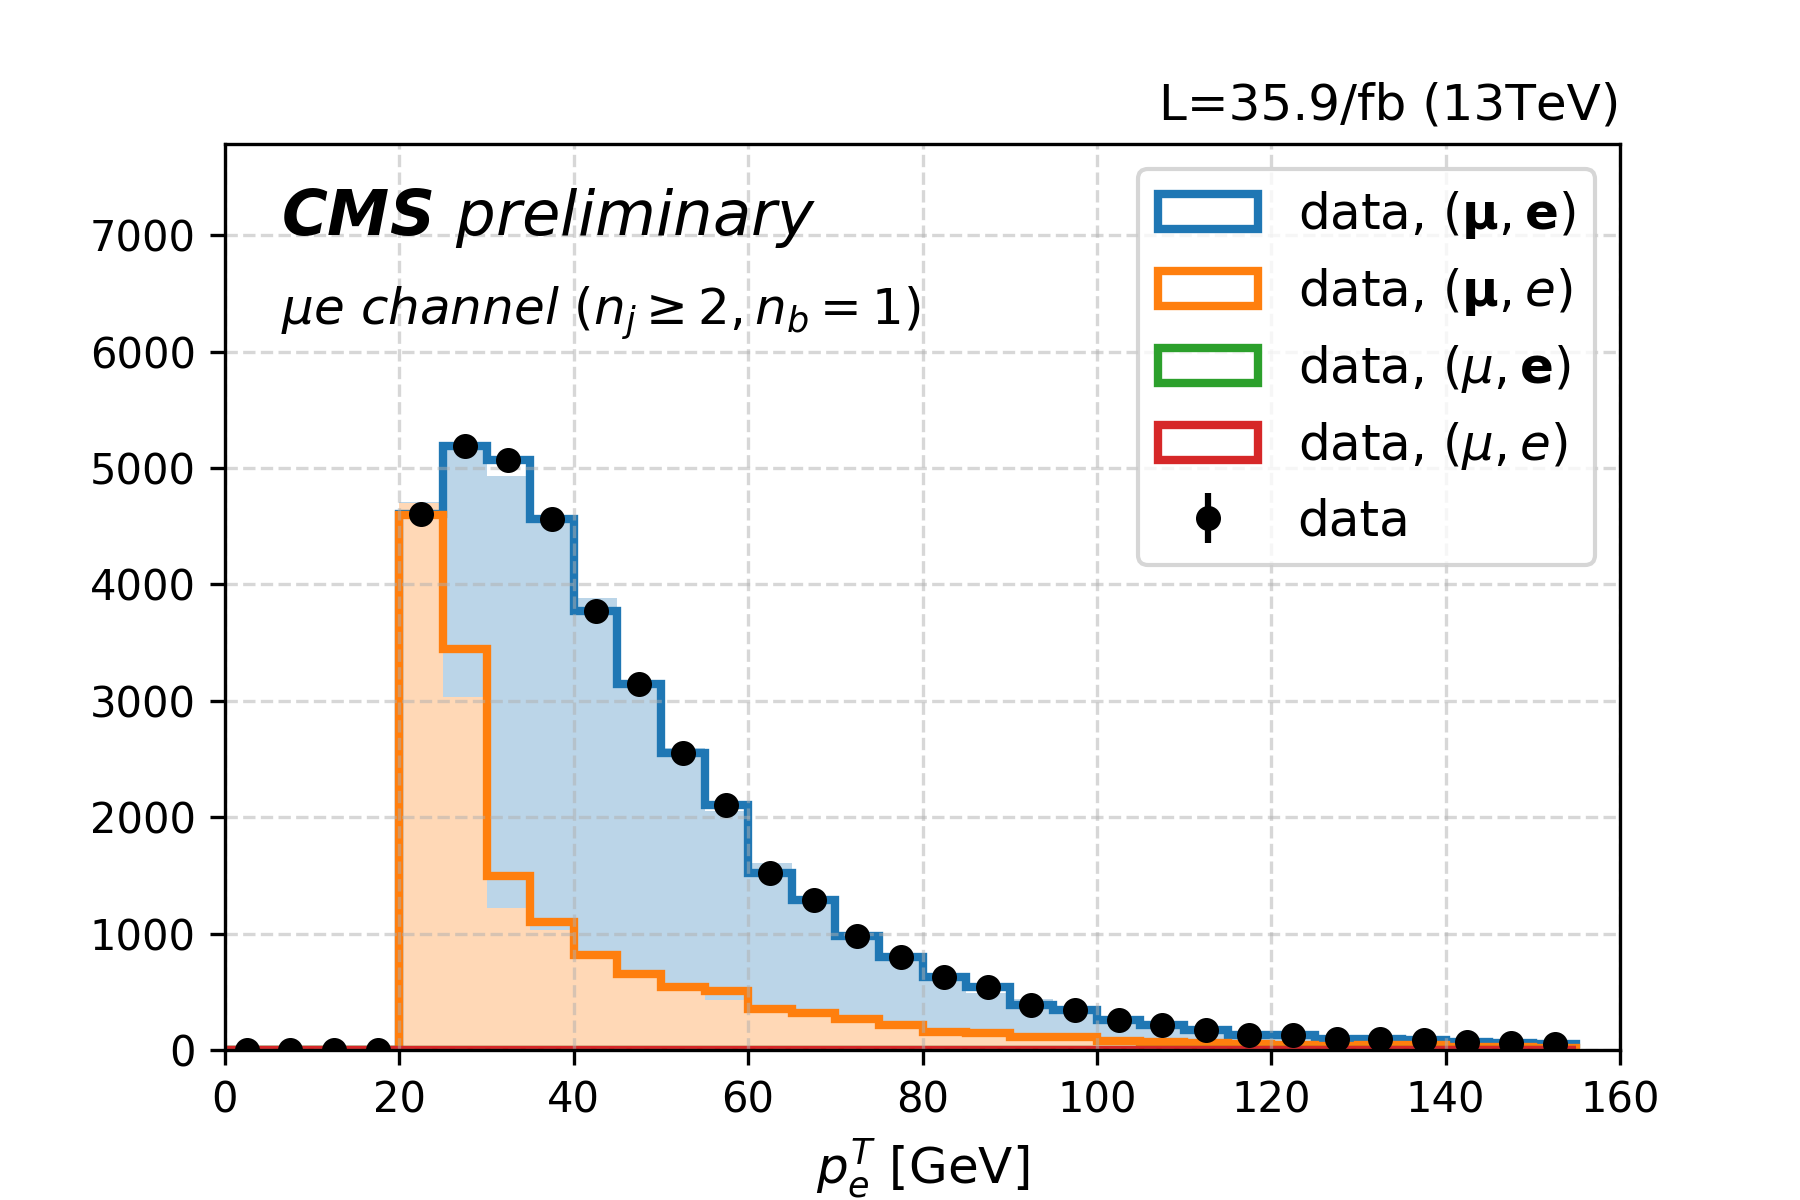
\includegraphics[width=0.49\textwidth]{chapters/Analysis/sectionSelection/figures/trgLep_emu.png}
%     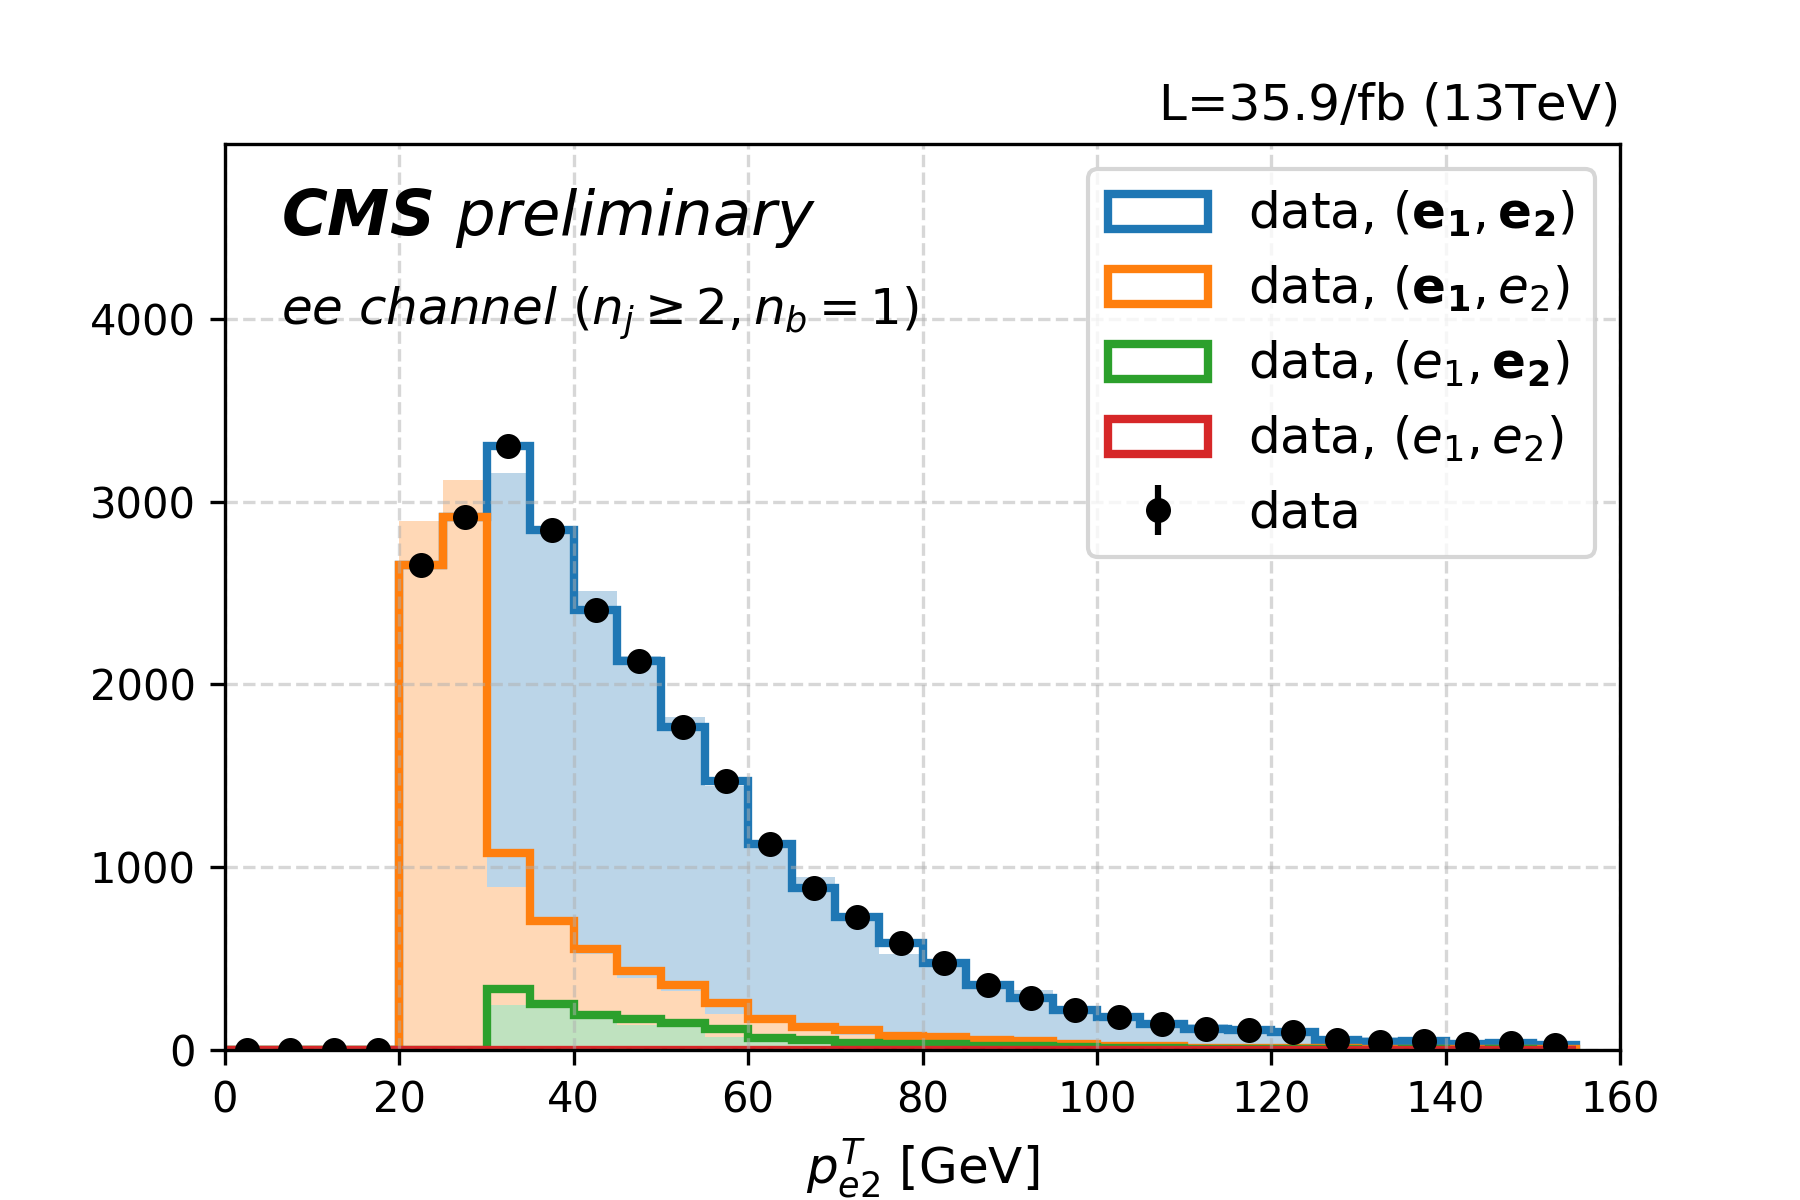
\includegraphics[width=0.49\textwidth]{chapters/Analysis/sectionSelection/figures/trgLep_ee.png}
%     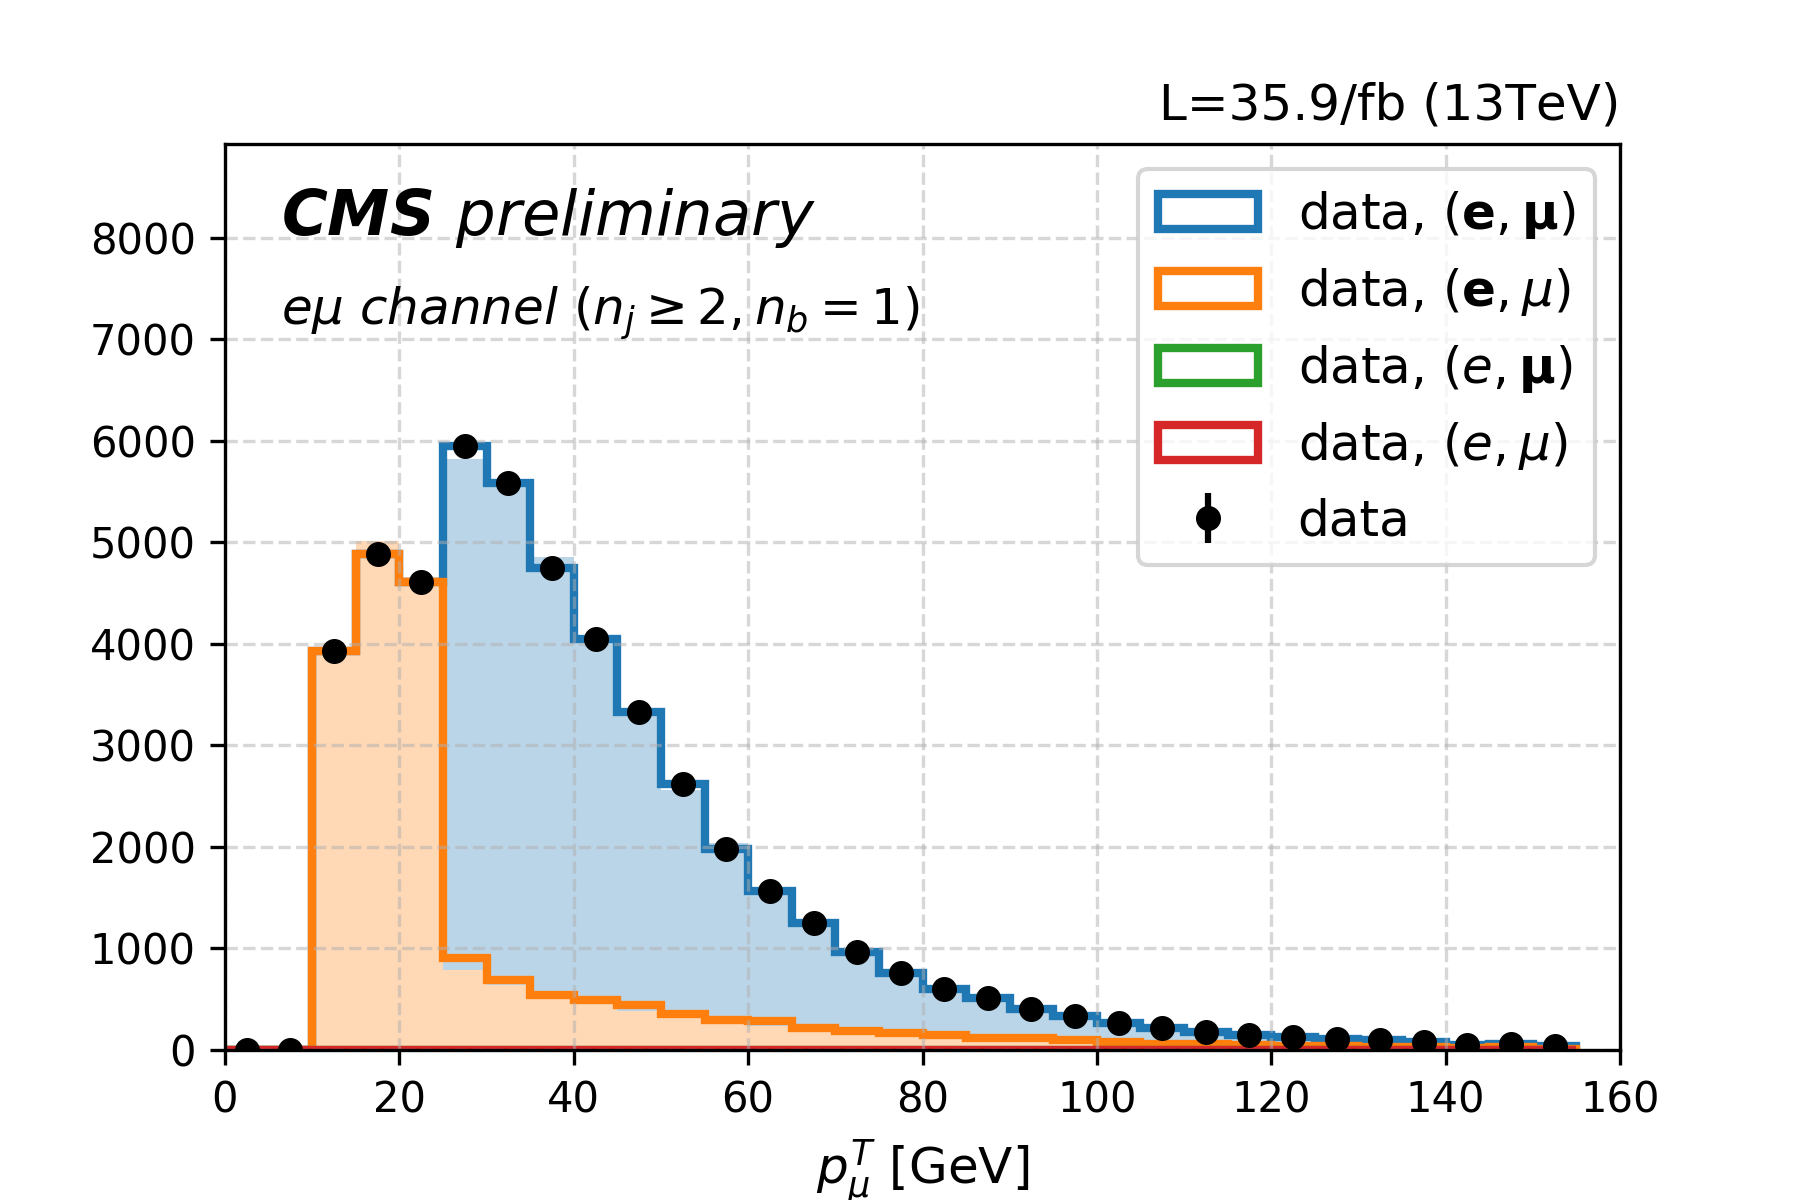
\includegraphics[width=0.49\textwidth]{chapters/Analysis/sectionSelection/figures/trgLep_emu2.png}
%     \caption{caption}
%     \label{fig:analysis:selection:trigger}
% \end{figure}




\begin{sidewaystable}[ht]
    \centering
    \setlength{\tabcolsep}{0.4em}
    \renewcommand{\arraystretch}{1.5}

    \caption{Composition of accepted $t\bar{t}$+$tW$ events, breakdown by 21 WW decay.  Values are in percent.}
    \resizebox{\textwidth}{!}{
    \begin{tabular}{|l|cc|cc|cc|cc|cc|cc|cc|cc|}
    
    
    \hline
    channel & \multicolumn{2}{|c|}{$\mu e$} & \multicolumn{2}{c|}{$\mu\mu$} & \multicolumn{2}{|c|}{$\mu \tau$} & \multicolumn{2}{|c|}{$\mu$+jets} & \multicolumn{2}{|c|}{$ee$} & \multicolumn{2}{|c|}{$e\mu$} & \multicolumn{2}{|c|}{$e \tau$} & \multicolumn{2}{|c|}{$e+jets$} \\
    \hline
    $\rm n_{b tag}$ & $n_b=1$ & $n_b\geq2$ & $n_b=1$ & $n_b\geq2$ & $n_b=1$ & $n_b\geq2$ & $n_b=1$ & $n_b\geq2$ & $n_b=1$ & $n_b\geq2$ & $n_b=1$ & $n_b\geq2$ & $n_b=1$ & $n_b\geq2$ & $n_b=1$ & $n_b\geq2$ \\ 
    \hline
    
    $tt/tW \to ee$                     &   -- &   -- &   -- &   -- &   -- &   -- &   -- &   -- & 87.4 & 87.8 &   -- &   -- &  0.7 &   -- &  3.1 &  3.1 \\ 
    $tt/tW \to \mu\mu$                 &   -- &   -- & 81.6 & 83.0 &   -- &   -- &  1.3 &  1.2 &   -- &   -- &   -- &   -- &   -- &   -- &   -- &   -- \\ 
    $tt/tW \to e\mu$                   & 86.5 & 87.0 &   -- &   -- &  0.8 &  0.5 &  3.3 &  3.3 &   -- &   -- & 82.7 & 84.1 &   -- &   -- &  1.4 &  1.4 \\ 
    $tt/tW \to \tau_{e}\tau_{e}$       &   -- &   -- &   -- &   -- &   -- &   -- &   -- &   -- &   -- &   -- &   -- &   -- &   -- &   -- &   -- &   -- \\ 
    $tt/tW \to \tau_{\mu}\tau_{\mu}$   &   -- &   -- &  0.7 &  0.6 &   -- &   -- &   -- &   -- &   -- &   -- &   -- &   -- &   -- &   -- &   -- &   -- \\ 
    $tt/tW \to \tau_{e}\tau_{\mu}$     &   -- &   -- &   -- &   -- &   -- &   -- &   -- &   -- &   -- &   -- &  0.6 &  0.6 &   -- &   -- &   -- &   -- \\ 
    $tt/tW \to \tau_{e}\tau_{h}$       &   -- &   -- &   -- &   -- &   -- &   -- &   -- &   -- &   -- &   -- &   -- &   -- &  3.1 &  3.2 &   -- &   -- \\ 
    $tt/tW \to \tau_{\mu}\tau_{h}$     &   -- &   -- &   -- &   -- &  3.2 &  3.6 &   -- &   -- &   -- &   -- &   -- &   -- &   -- &   -- &   -- &   -- \\ 
    $tt/tW \to \tau_{h}\tau_{h}$       &   -- &   -- &   -- &   -- &   -- &   -- &   -- &   -- &   -- &   -- &   -- &   -- &   -- &   -- &   -- &   -- \\ 
    $tt/tW \to e\tau_{e}$              &   -- &   -- &   -- &   -- &   -- &   -- &   -- &   -- & 11.7 & 11.5 &   -- &   -- &   -- &   -- &  0.8 &  0.8 \\ 
    $tt/tW \to e\tau_{\mu}$            &  4.1 &  4.0 &   -- &   -- &   -- &   -- &   -- &   -- &   -- &   -- & 11.2 & 11.0 &   -- &   -- &   -- &   -- \\ 
    $tt/tW \to e\tau_{h}$              &   -- &   -- &   -- &   -- &   -- &   -- &   -- &   -- &   -- &   -- &   -- &   -- & 57.5 & 63.6 &  3.4 &  3.6 \\ 
    $tt/tW \to \mu\tau_{e}$            &  8.3 &  8.2 &   -- &   -- &   -- &   -- &  0.6 &  0.7 &   -- &   -- &  3.6 &  3.6 &   -- &   -- &   -- &   -- \\ 
    $tt/tW \to \mu\tau_{\mu}$          &   -- &   -- & 15.7 & 15.8 &   -- &   -- &   -- &   -- &   -- &   -- &   -- &   -- &   -- &   -- &   -- &   -- \\ 
    $tt/tW \to \mu\tau_{h}$            &   -- &   -- &   -- &   -- & 57.4 & 63.6 &  3.4 &  3.6 &   -- &   -- &   -- &   -- &   -- &   -- &   -- &   -- \\ 
    $tt/tW \to eh$                     &   -- &   -- &   -- &   -- &   -- &   -- &   -- &   -- &   -- &   -- &  1.6 &   -- & 35.9 & 30.5 & 85.6 & 85.4 \\ 
    $tt/tW \to \mu h$                  &   -- &   -- &  1.7 &  0.5 & 35.7 & 30.1 & 85.3 & 85.3 &   -- &   -- &   -- &   -- &   -- &   -- &   -- &   -- \\ 
    $tt/tW \to \tau_{e}h$              &   -- &   -- &   -- &   -- &   -- &   -- &   -- &   -- &   -- &   -- &   -- &   -- &  1.9 &  1.6 &  4.8 &  4.7 \\ 
    $tt/tW \to \tau_{\mu}h$            &   -- &   -- &   -- &   -- &  2.1 &  1.6 &  5.0 &  4.9 &   -- &   -- &   -- &   -- &   -- &   -- &   -- &   -- \\ 
    $tt/tW \to \tau_{h}h$              &   -- &   -- &   -- &   -- &   -- &   -- &   -- &   -- &   -- &   -- &   -- &   -- &   -- &   -- &   -- &   -- \\ 
    $tt/tW \to hh$                     &   -- &   -- &   -- &   -- &   -- &   -- &   -- &   -- &   -- &   -- &   -- &   -- &   -- &   -- &   -- &   -- \\ 

    \hline
    \end{tabular}}
    \label{tab:analysis:selection:signal_breakdown}
    
\end{sidewaystable}

\begin{sidewaystable}[ht]
    \centering
    % \rule{1.5\textwidth}{0.8\textwidth}
    % \toprule
    \setlength{\tabcolsep}{0.0em}
    \renewcommand{\arraystretch}{2}
    \footnotesize
    \begin{tabular}{l|cccccccc|cc}
    \hline
        & QCD & VV  & $\gamma$ & Z & W & t & tW & tt & total & data      \\
    \hline
    
    $\mu e$, $n_b=1$                   &       --$\pm$     -- &     90.3$\pm$    4.2 &      0.9$\pm$    0.9 &    202.7$\pm$   37.6 &     13.4$\pm$    5.1 &      9.5$\pm$    2.6 &   2107.6$\pm$   53.1 &  38871.4$\pm$   87.5 &  41295.8$\pm$  109.2 &  41047.0$\pm$  202.6 \\ 
    $\mu e$, $n_b\geq2$                &       --$\pm$     -- &      5.9$\pm$    1.0 &       --$\pm$     -- &       --$\pm$     -- &      3.1$\pm$    2.2 &      2.3$\pm$    1.6 &    625.7$\pm$   28.9 &  22647.7$\pm$   66.8 &  23270.9$\pm$   74.1 &  23918.0$\pm$  154.7 \\ 
    \hline
    $\mu\mu$, $n_b=1$                  &       --$\pm$     -- &    370.4$\pm$    5.8 &      4.1$\pm$    1.8 &  18046.9$\pm$  455.4 &     52.4$\pm$   11.7 &     55.8$\pm$    6.7 &   3406.2$\pm$   68.8 &  62266.6$\pm$  112.4 &  84202.3$\pm$  474.3 &  84284.0$\pm$  290.3 \\ 
    $\mu\mu$, $n_b\geq2$               &       --$\pm$     -- &     45.8$\pm$    1.5 &      0.0$\pm$    0.0 &   1945.7$\pm$  142.0 &      3.6$\pm$    2.6 &      3.9$\pm$    1.8 &    959.3$\pm$   36.2 &  35685.2$\pm$   85.1 &  38643.4$\pm$  169.6 &  39253.0$\pm$  198.1 \\ 
    \hline
    $\mu\tau$, $n_b=1$                 &   1130.7$\pm$  108.8 &     52.3$\pm$    2.6 &     11.8$\pm$    3.2 &    866.7$\pm$   78.7 &    730.8$\pm$   42.9 &    182.6$\pm$   12.4 &   1291.0$\pm$   41.9 &  18430.0$\pm$   60.6 &  22695.9$\pm$  159.6 &  21621.0$\pm$  147.0 \\ 
    $\mu\tau$, $n_b\geq2$              &    346.6$\pm$   51.5 &      5.5$\pm$    0.7 &      0.9$\pm$    0.8 &    103.6$\pm$   29.6 &     56.9$\pm$   14.4 &     36.8$\pm$    5.6 &    322.6$\pm$   21.0 &   9647.6$\pm$   43.7 &  10520.4$\pm$   78.3 &   9934.0$\pm$   99.7 \\ 
    \hline
    $\mu$+jets, $n_b=1$                &  24300.4$\pm$ 3404.9 &    371.0$\pm$    5.2 &   1501.2$\pm$   67.5 &   7533.2$\pm$  265.9 &  49248.1$\pm$  327.3 &   8484.6$\pm$   85.3 &  24447.8$\pm$  187.0 & 514064.6$\pm$  327.2 & 629950.9$\pm$ 3453.3 & 630704.0$\pm$  794.2 \\ 
    $\mu$+jets, $n_b\geq2$             &   4650.7$\pm$ 1399.5 &     61.4$\pm$    2.0 &    248.3$\pm$   31.8 &   1331.9$\pm$  114.0 &   6524.2$\pm$  118.8 &   5172.2$\pm$   66.7 &  10335.6$\pm$  121.4 & 356185.1$\pm$  272.2 & 384509.5$\pm$ 1442.2 & 385397.0$\pm$  620.8 \\ 
    \hline
    $e e$, $n_b=1$                     &       --$\pm$     -- &    138.2$\pm$    3.6 &      2.8$\pm$    1.2 &   4726.5$\pm$  215.7 &      5.4$\pm$    2.8 &      1.1$\pm$    0.8 &   1382.0$\pm$   42.7 &  23447.3$\pm$   66.9 &  29703.3$\pm$  229.9 &  29491.0$\pm$  171.7 \\ 
    $e e$, $n_b\geq2$                  &       --$\pm$     -- &     16.2$\pm$    0.9 &      0.1$\pm$    0.1 &    500.5$\pm$   67.8 &      3.7$\pm$    2.6 &      2.1$\pm$    1.2 &    371.4$\pm$   22.1 &  13412.7$\pm$   50.7 &  14306.6$\pm$   87.5 &  14334.0$\pm$  119.7 \\ 
    \hline
    $e\mu$, $n_b=1$                    &       --$\pm$     -- &    127.2$\pm$    4.9 &     25.5$\pm$   13.2 &    411.9$\pm$   52.7 &     32.8$\pm$    7.2 &     37.6$\pm$    5.4 &   2917.6$\pm$   62.7 &  49878.6$\pm$   99.2 &  53431.1$\pm$  129.8 &  52362.0$\pm$  228.8 \\ 
    $e\mu$, $n_b\geq2$                 &       --$\pm$     -- &      9.0$\pm$    1.3 &      1.9$\pm$    1.1 &     59.0$\pm$   19.5 &      6.5$\pm$    3.2 &      6.1$\pm$    2.2 &    837.9$\pm$   33.8 &  28374.1$\pm$   74.9 &  29294.5$\pm$   84.6 &  29860.0$\pm$  172.8 \\ 
    \hline
    $e\tau$, $n_b=1$                   &    874.2$\pm$   90.3 &     38.0$\pm$    2.1 &    194.5$\pm$   38.8 &    677.8$\pm$   69.3 &    456.3$\pm$   32.9 &    125.3$\pm$   10.0 &    908.2$\pm$   34.6 &  12884.7$\pm$   49.7 &  16159.1$\pm$  139.0 &  15309.0$\pm$  123.7 \\ 
    $e\tau$, $n_b\geq2$                &     94.2$\pm$   46.3 &      3.0$\pm$    0.4 &     10.0$\pm$    2.9 &     53.4$\pm$   21.3 &     28.7$\pm$    8.5 &     43.4$\pm$    6.0 &    196.1$\pm$   15.9 &   6682.4$\pm$   35.8 &   7111.3$\pm$   65.1 &   7006.0$\pm$   83.7 \\ 
    \hline
    $e$+jets, $n_b=1$                  &  25625.1$\pm$ 2941.3 &    494.9$\pm$    5.1 &  12035.7$\pm$  173.0 &  13119.8$\pm$  323.2 &  34481.3$\pm$  266.1 &   5786.3$\pm$   68.8 &  17454.7$\pm$  154.8 & 360917.6$\pm$  268.5 & 469915.4$\pm$ 2992.9 & 464543.0$\pm$  681.6 \\ 
    $e$+jets, $n_b\geq2$               &   3327.4$\pm$ 1476.4 &     84.5$\pm$    2.0 &   2095.3$\pm$   78.4 &   2520.8$\pm$  138.5 &   4696.3$\pm$   98.0 &   3524.2$\pm$   53.7 &   7616.3$\pm$  102.3 & 249557.0$\pm$  223.4 & 273421.8$\pm$ 1509.3 & 274162.0$\pm$  523.6 \\ 
    \hline

    \end{tabular}
    \caption{Estimates of the yields. The estimate of the expected yield is compared to
    the yield observed from data.  Uncertainties are statistical only.
    \label{tab:yields}}
\end{sidewaystable}

\begin{sidewaystable}[]
    \centering
    \setlength{\tabcolsep}{0.4em}
    \renewcommand{\arraystretch}{1.5}
    
    \caption{Estimates of the yields for various processes in
    the $e\tau$ and $\mu\tau$ categories broken down by the number of b tags.
    The estimate of the expected yield is compared to the yield observed
    from data.  Uncertainties are statistical only.}
    
    \resizebox{\textwidth}{!}{
        \begin{tabular}{l|ccccccc|cc}
        \hline
                                        & QCD                  & Diboson (non-WW) & WW               & Z                      & W                    & tW                & $\sf t\bar{t}$     & Expected               & Observed \\
        \hline
        \multicolumn{10}{l}{$e\tau$}   \\
        \hline
        $N_{j} = 0, N_{b} = 0$          & $14609.7 \pm 843.7$  & $11.7 \pm 1.4$   & $102.2 \pm 7.2$  & $30670.4 \pm 3175.9$   & $9505.8 \pm 594.4$   & $11.1 \pm 3.7$    & $29.7 \pm 2.8$     & $54940.5 \pm 3339.4$   & $55591$  \\
        $N_{j} = 1, N_{b} = 0$          & $1512.7 \pm 125.2$   & $10.0 \pm 1.2$   & $20.9 \pm 2.3$   & $3237.1 \pm 355.2$     & $1159.9 \pm 98.0$    & $20.8 \pm 5.2$    & $76.3 \pm 5.7$     & $6037.5 \pm 389.2$     & $6074$   \\
        $N_{j} \geq 2, N_{b} = 0$       & $5519.7 \pm 363.2$   & $233.6 \pm 24.3$ & $269.8 \pm 16.8$ & $6721.8 \pm 724.1$     & $6906.0 \pm 410.6$   & $551.2 \pm 40.4$  & $5933.6 \pm 333.3$ & $26135.7 \pm 968.7$    & $25788$  \\
        $N_{j} = 1, N_{b} = 1$          & $789.5 \pm 77.4$     & $8.0 \pm 1.0$    & $16.4 \pm 2.0$   & $725.6 \pm 99.6$       & $650.5 \pm 60.3$     & $675.5 \pm 47.6$  & $3381.9 \pm 190.7$ & $6247.5 \pm 241.2$     & $6256$   \\
        $N_{j} = 2, N_{b} = 1$          & $421.6 \pm 59.9$     & $11.7 \pm 1.3$   & $10.8 \pm 1.6$   & $424.7 \pm 69.2$       & $305.0 \pm 33.4$     & $538.3 \pm 39.7$  & $5994.7 \pm 336.8$ & $7706.7 \pm 352.8$     & $7388$   \\
        $N_{j} \geq 3, N_{b} = 1$       & $315.4 \pm 56.0$     & $13.1 \pm 1.5$   & $5.0 \pm 1.0$    & $212.1 \pm 42.9$       & $169.3 \pm 23.1$     & $302.1 \pm 25.7$  & $6021.4 \pm 338.2$ & $7038.5 \pm 347.2$     & $6660$   \\
        $N_{j} = 2, N_{b} \geq 2$       & $48.4 \pm 16.4$      & $1.1 \pm 0.2$    & $0.3 \pm 0.2$    & $18.8 \pm 15.9$        & $10.6 \pm 5.8$       & $83.4 \pm 11.1$   & $2606.9 \pm 147.4$ & $2769.5 \pm 149.7$     & $2683$   \\
        $N_{j} \geq 3, N_{b} \geq 2$    & $81.3 \pm 28.8$      & $1.8 \pm 0.3$    & $0.3 \pm 0.2$    & $55.2 \pm 14.0$        & $18.0 \pm 6.9$       & $87.8 \pm 11.5$   & $3574.9 \pm 201.5$ & $3819.4 \pm 204.5$     & $3704$   \\
        \hline
        \multicolumn{10}{l}{$\mu\tau$} \\
        \hline
        $N_{j} = 0, N_{b} = 0$          & $19581.5 \pm 1133.6$ & $27.6 \pm 3.1$   & $244.6 \pm 15.3$ & $103926.9 \pm 10727.5$ & $20342.3 \pm 1205.2$ & $19.3 \pm 5.0$    & $66.2 \pm 5.1$     & $144208.5 \pm 10854.4$ & $146128$ \\
        $N_{j} = 1, N_{b} = 0$          & $2255.6 \pm 167.9$   & $24.0 \pm 2.6$   & $37.0 \pm 3.4$   & $8216.3 \pm 868.5$     & $2470.3 \pm 177.3$   & $33.8 \pm 6.8$    & $162.4 \pm 10.6$   & $13199.4 \pm 902.2$    & $13293$  \\
        $N_{j} \geq 2, N_{b} = 0$       & $5467.2 \pm 372.9$   & $313.5 \pm 32.5$ & $413.2 \pm 24.9$ & $10752.1 \pm 1139.7$   & $10989.1 \pm 640.3$  & $879.2 \pm 59.4$  & $9261.1 \pm 519.4$ & $38075.4 \pm 1457.1$   & $38184$  \\
        $N_{j} = 1, N_{b} = 1$          & $1452.3 \pm 113.6$   & $12.3 \pm 1.4$   & $27.8 \pm 2.8$   & $1632.3 \pm 193.8$     & $1199.1 \pm 96.4$    & $1112.9 \pm 72.6$ & $5266.7 \pm 296.1$ & $10703.3 \pm 390.8$    & $10628$  \\
        $N_{j} = 2, N_{b} = 1$          & $709.7 \pm 75.4$     & $17.6 \pm 1.9$   & $18.1 \pm 2.1$   & $708.4 \pm 101.7$      & $568.1 \pm 50.5$     & $769.3 \pm 53.1$  & $9493.5 \pm 532.4$ & $12284.6 \pm 552.1$    & $12048$  \\
        $N_{j} \geq 3, N_{b} = 1$       & $438.5 \pm 70.7$     & $19.5 \pm 2.1$   & $9.7 \pm 1.5$    & $384.5 \pm 62.6$       & $292.9 \pm 32.0$     & $480.7 \pm 36.5$  & $9413.5 \pm 527.9$ & $11039.3 \pm 538.5$    & $10314$  \\
        $N_{j} = 2, N_{b} \geq 2$       & $111.1 \pm 19.9$     & $1.7 \pm 0.2$    & $1.0 \pm 0.4$    & $58.6 \pm 23.6$        & $56.0 \pm 16.9$      & $153.8 \pm 16.5$  & $4157.7 \pm 234.1$ & $4539.9 \pm 237.3$     & $4321$   \\
        $N_{j} \geq 3, N_{b} \geq 2$    & $117.5 \pm 35.6$     & $3.0 \pm 0.4$    & $1.4 \pm 0.5$    & $79.4 \pm 22.2$        & $18.1 \pm 6.9$       & $157.9 \pm 16.7$  & $5599.2 \pm 314.7$ & $5976.5 \pm 318.0$     & $5705$   \\
        \hline
    \end{tabular}}

    \label{tab:yields_ltau}
\end{sidewaystable}



\FloatBarrier




\section{Calibrations}
\label{sec:analysis:calibration}



\subsection{Measurement of Scale Factors for the Single Electron Trigger}
\label{sec:analysis:calibration:eTriggerEff}


% \subsection{Measurement Approach}

The data for the measurement of \PW branching fraction is triggered with single electron and single muon trigger. The difference between the trigger efficiencies in the simulation and data is accounted for by applying scale factors to the event weights of simulation. While the scale factors are provided by POG for the correction of single muon trigger efficiencies, those for the single electron has to be measured. 

Single electron trigger, \texttt{HLT\_Ele27\_WPTight\_Gsf}, is used in the $ee$, $e\mu$, $e\tau_h$, $e$+jets channels. Here a customized measurement of scale factor and the associated uncertainties of \texttt{HLT\_Ele27\_WPTight\_Gsf} trigger is performed based on 2016 re-reco dataset with the tag-prob approach. The uncertainty of the scale factor includes both statistical and systematical uncertainty, where systematical uncertainty are estimated by"two shifts":

\begin{enumerate}
  \item shift up the tagging electron by 10 GeV to simulate a different trigger. This estimates the systematical effect that some L1 seed could have a threshold of 32 GeV.
  \item shift the probing electron pT up and down by 0.5 GeV. This estimates the effect of the electron \pt resolution.
\end{enumerate}


\begin{figure}
    \centering
    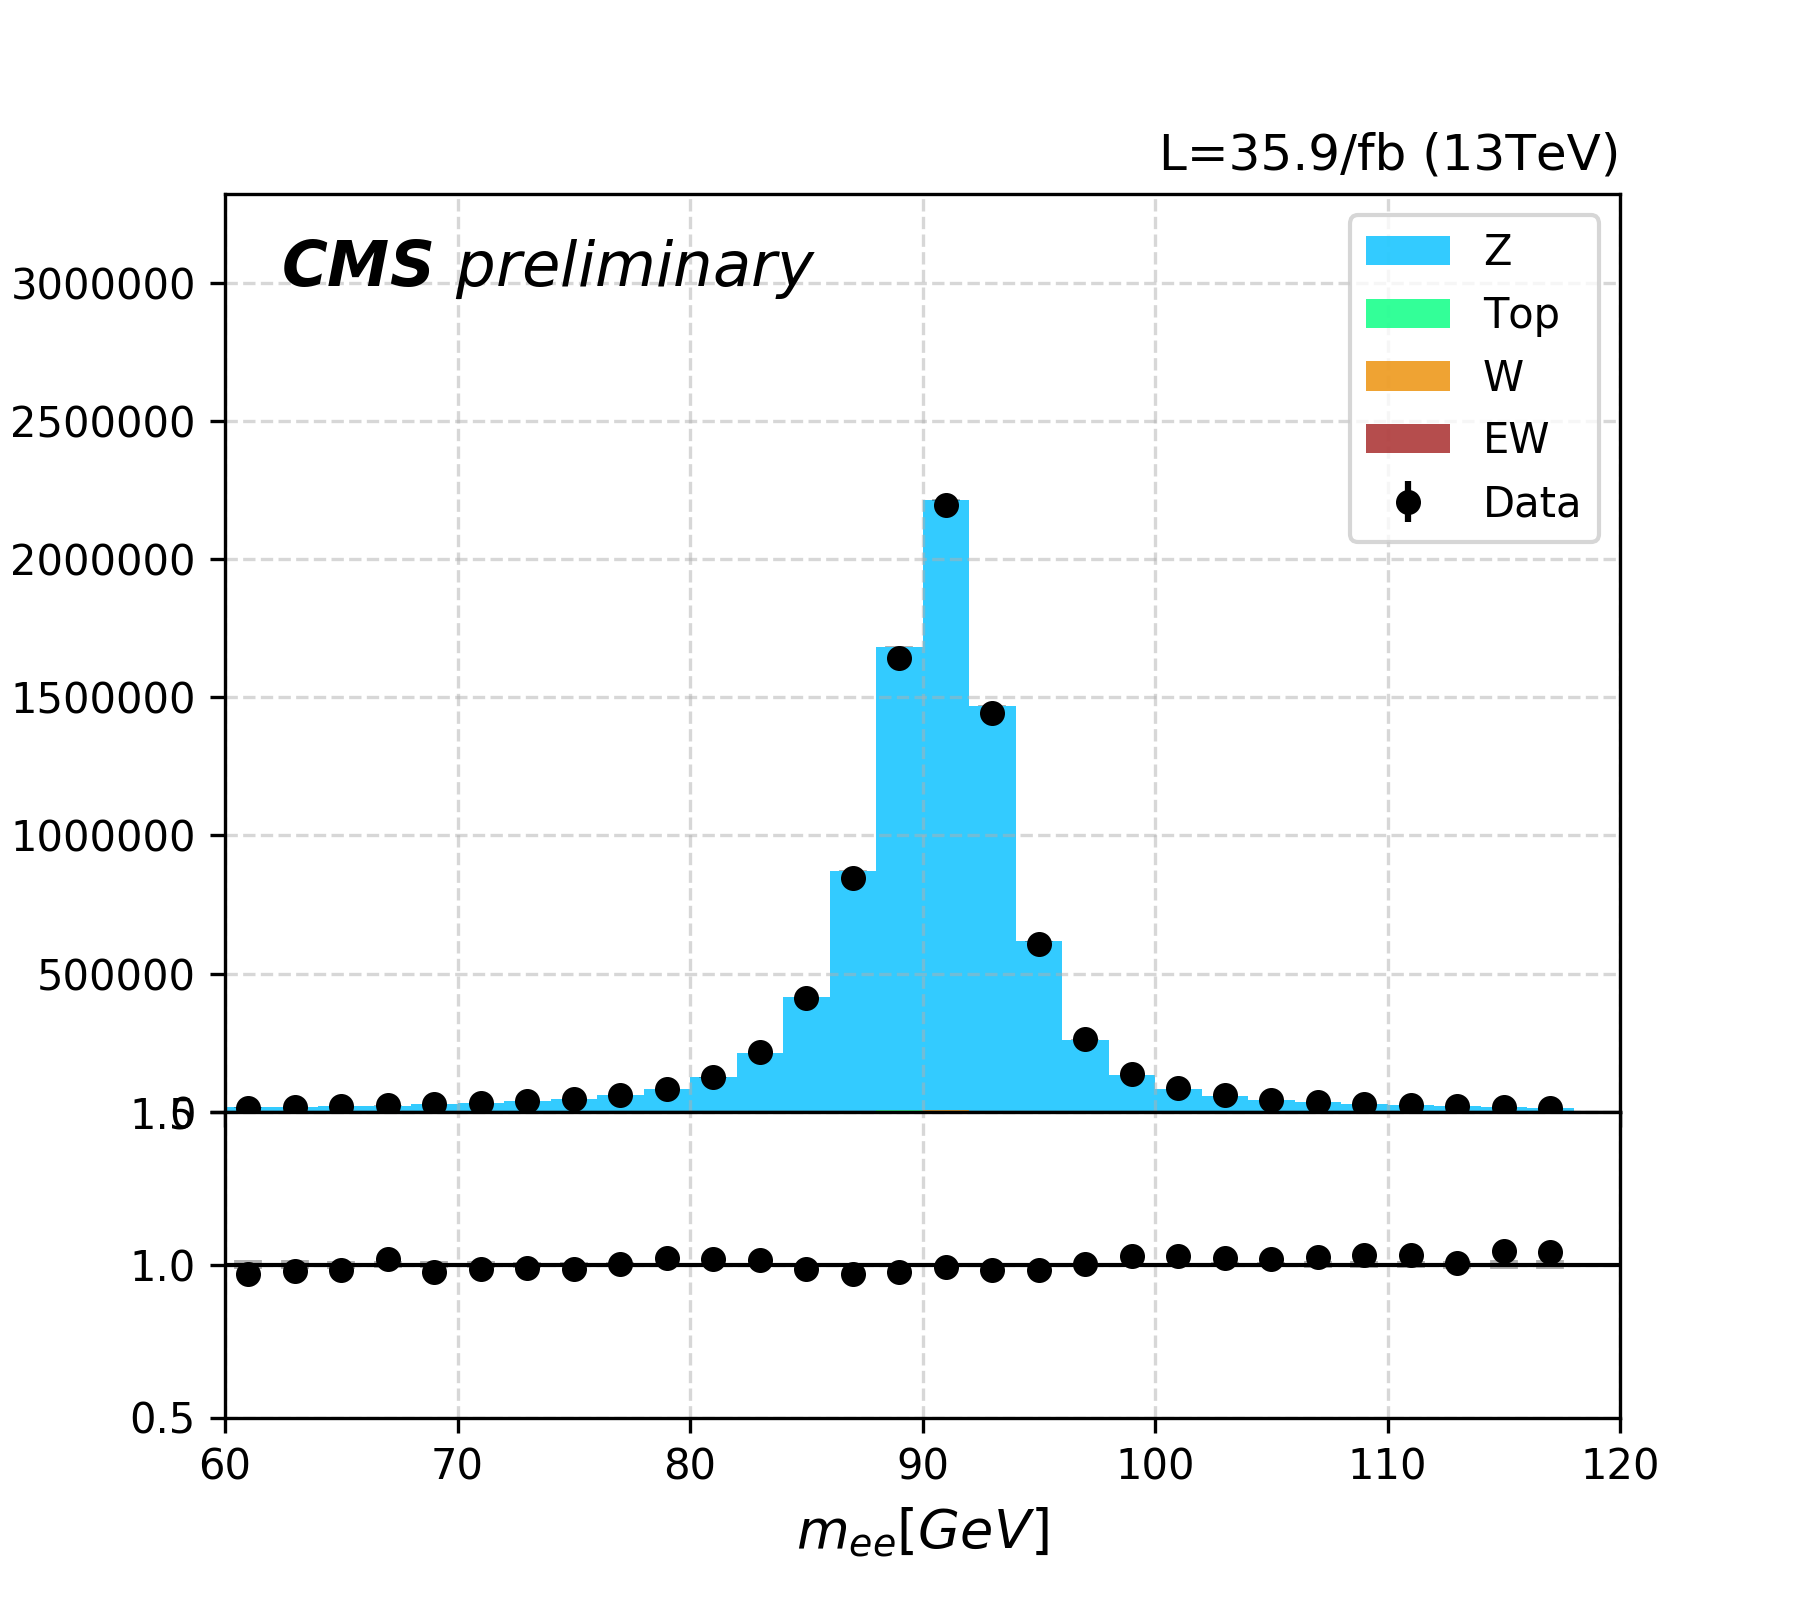
\includegraphics[width=0.6\textwidth]{chapters/Analysis/sectionCalibration/figures/eTrigger/dileptonMass_tag30.png}
    \caption{$m_{ee}$ of the selected events for the measurement of the SF of single-electron trigger efficiency.}
    \label{fig:appendix:ele27TriggerSF}
\end{figure}


The dataset used in the measurement is 2016 re-reco \texttt{SingleElectron} dataset with the golden certificate as luminosity mask. The simulations used in the measurement include \texttt{DYJETSToLL\_M-10to50\_amcatnlo}, \texttt{DYJETSToLL\_M-50\_amcatnlo} and \texttt{TT\_powheg}, reweighted to pile-up $\sigma_{mb} = 69.2\pm 2.3$ nb.

The electrons are selected with tight identification and tight particle-flow isolation with $p^T_e>20$ GeV and $|\eta_e|<2.5$. Corrections to the electrons in the simulation includes energy scale-smear, reconstruction and isolation. Among selected electrons, tagged electrons are defined as $p^T_e>30$ GeV and outside gap between barrel and endcap calorimeter $1.444<|\eta_e|<1.56$, and match with \texttt{HLT\_Ele27\_WPTight\_Gsf} triggering objects. Events are selected by requiring exactly 2 opposite electrons with at least 1 tagged electron and $60<m_{ee}<120$ GeV. This event selection yields a sample of events significantly dominated by Drell-Yan process. The distribution of $m_{ee}$ is shown in fig~\ref{fig:appendix:ele27TriggerSF}. The purity of Drell-Yan (DY) are very high in the selected events. Thus a signal-backgound fit is not necessary to get DY yields.





In each event, if one electron is tagged, the other become a prob. Each event provides either one or two tag-prob pairs. A prob is passing if it match with \texttt{HLT\_Ele27\_WPTight\_Gsf} triggering objects. The trigger efficiencies are calculated by the ratio between the number of passing probs over the total probs in $\pt-\eta$ bins, 

\begin{equation}
    \epsilon (\pt, \eta) = \frac{ N_{\rm passing} (\pt, \eta) } {  N_{\rm total} (\pt, \eta) }.
\end{equation}

\noindent The scale factors are derived by taking the ratio between efficiencies in the data over MC,
\begin{equation}
SF (\pt, \eta) = \frac{\epsilon_{\rm{data}} (\pt, \eta) }{\epsilon_{\rm{MC}} (\pt, \eta) }.
\end{equation}



% \subsection{Result of the Scale Factors}

In 2016 B-F, the data efficiency in the endcap decreases because there is a decrease of signal over noise ratio associated to loss of tracking hits caused by problems in the pre-amplifier of the APV chip. In the mid August 2016, this problem of Si-strip in endcap region is fixed by increase the drain speed of the pre-amplifier. Thus the trigger efficiencies are improved in 2016 GH. So the measurement of the scale factor of the trigger efficiency is divided into to two parts based on data taking periods, the 2016 B-F and 2016 GH.


The 2D maps of $\epsilon_{\rm{data}}$, $\epsilon_{\rm{MC}}$ and $SF$ in both 2016 B-F and 2016 GH are shown in Figure~\ref{fig:appendix:ele27SF}. Figure~\ref{fig:appendix:ele27SFperiods} shows the $SF$ in each 2016 data taking period, where the improvement in the G period is clear.



\begin{figure}
    \centering
    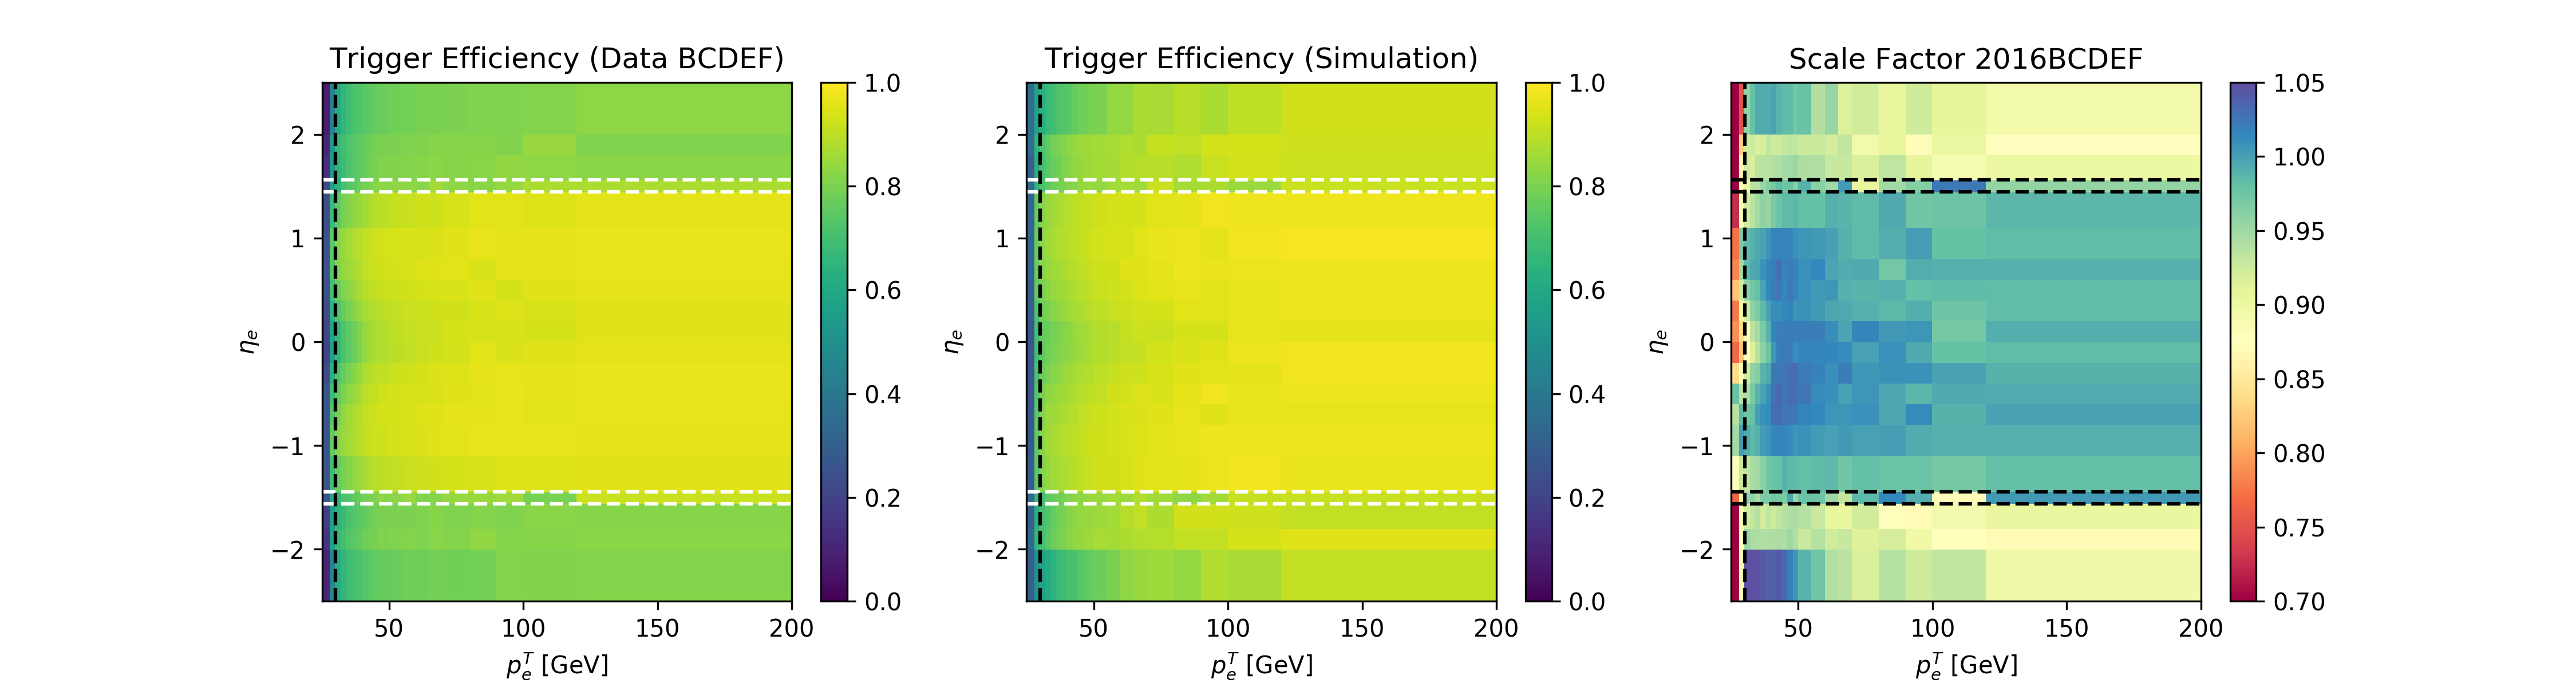
\includegraphics[width=0.99\textwidth]{chapters/Analysis/sectionCalibration/figures/eTrigger/eff2d_BCDEF.png}
    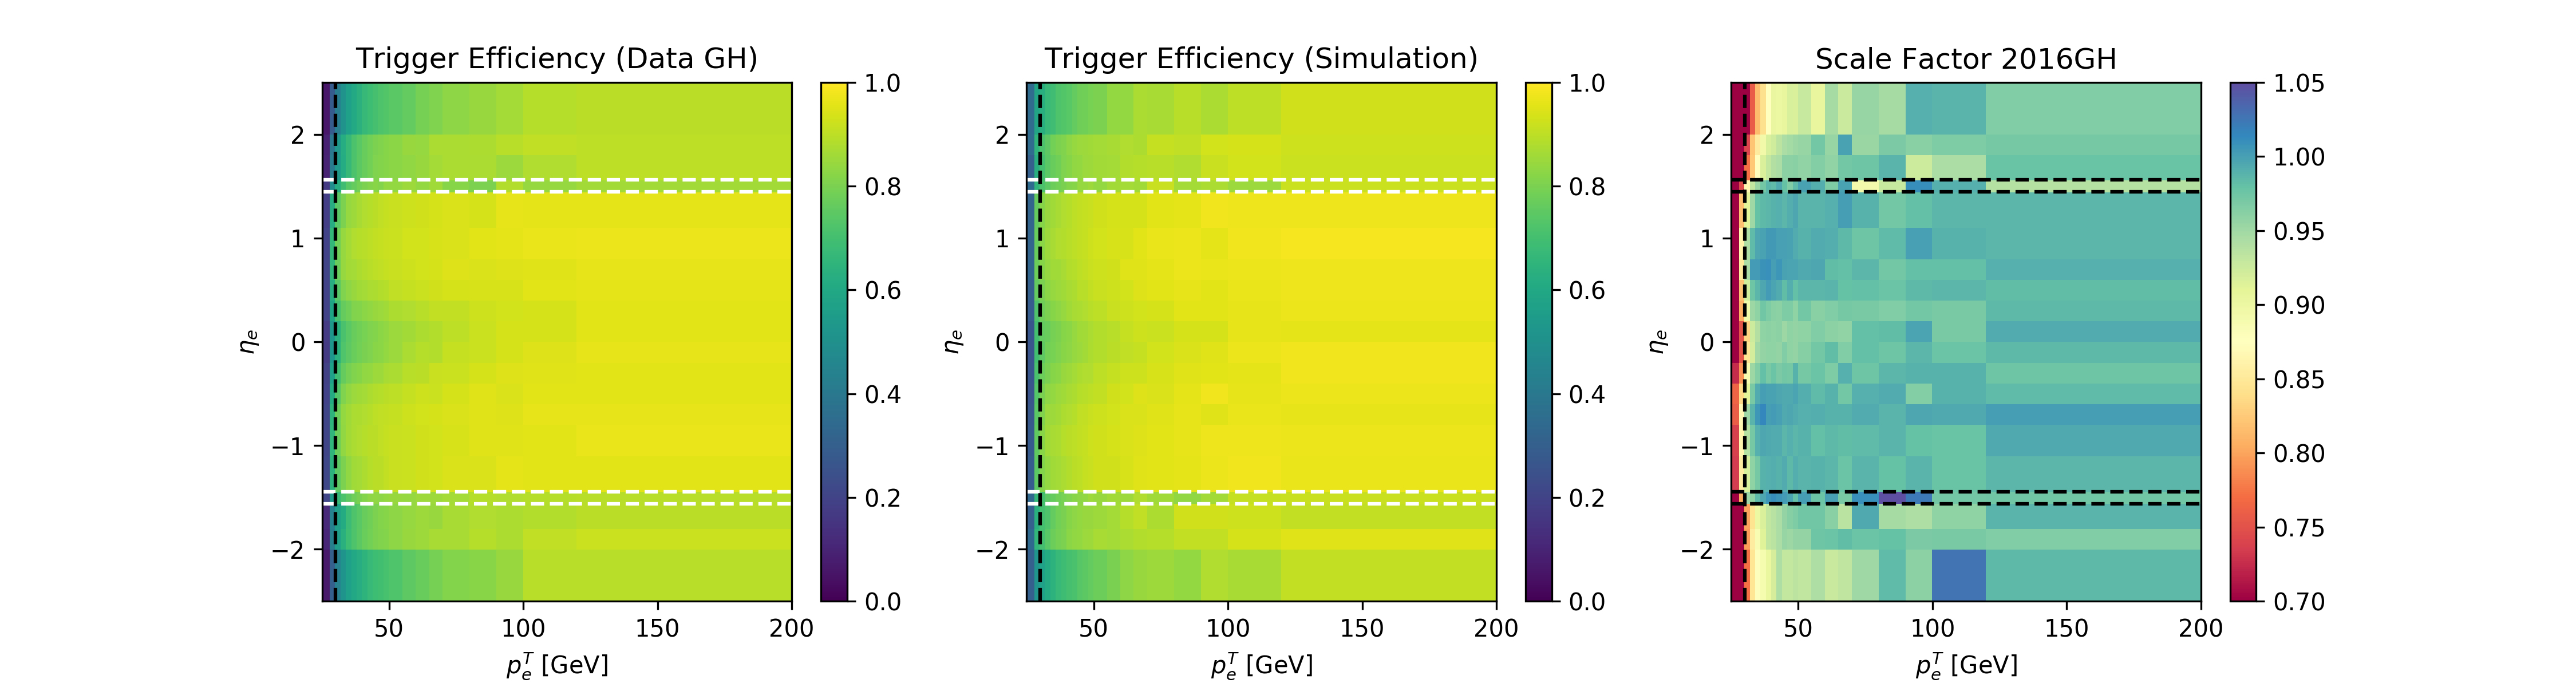
\includegraphics[width=0.99\textwidth]{chapters/Analysis/sectionCalibration/figures/eTrigger/eff2d_GH.png}
    \caption{The 2D maps of $\epsilon_{\rm{data}}$, $\epsilon_{\rm{MC}}$ and $SF$ in both 2016 B-F and 2016 GH.}
    \label{fig:appendix:ele27SF}
\end{figure}



\begin{figure}
    \centering
    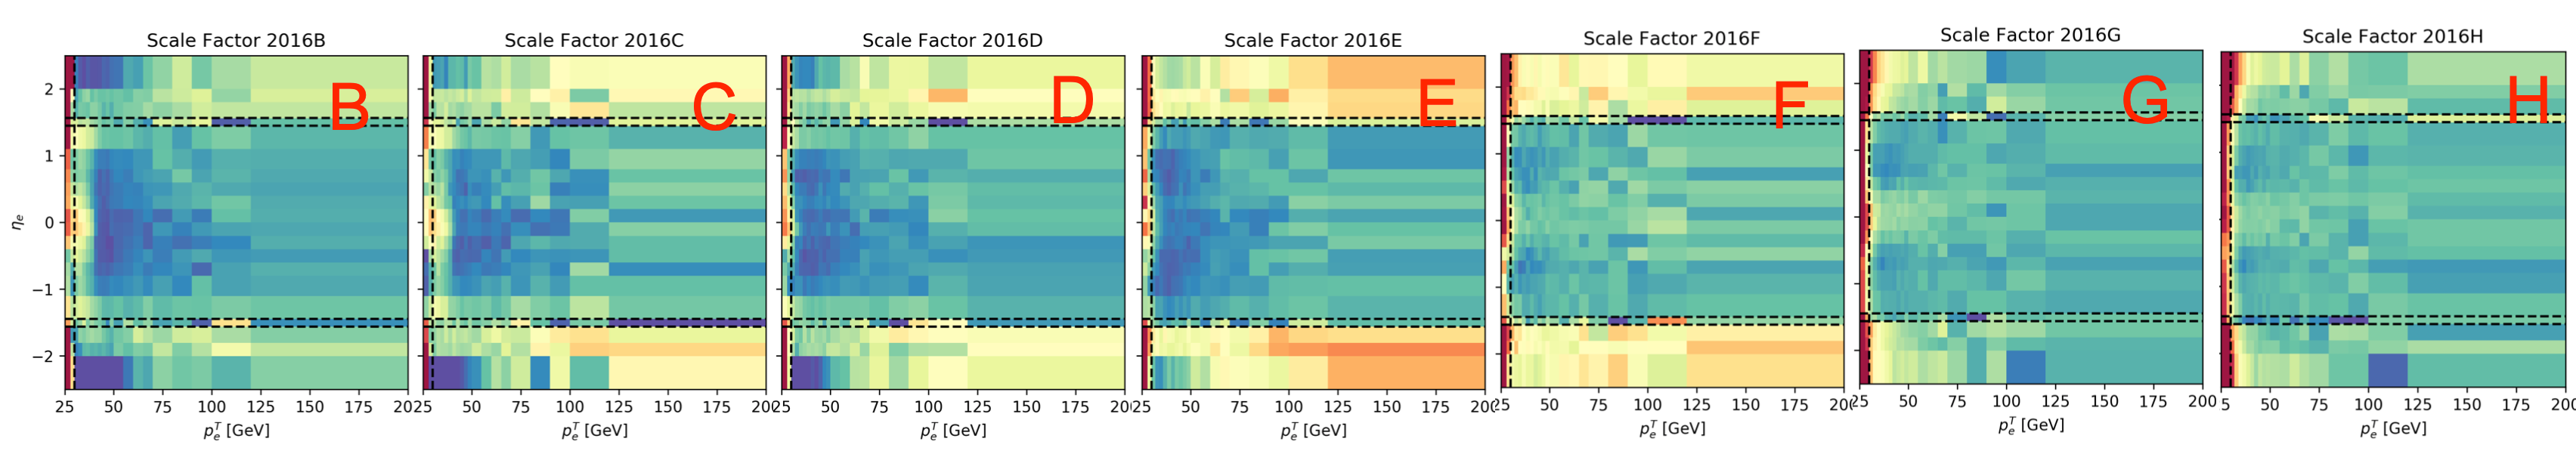
\includegraphics[width=0.99\textwidth]{chapters/Analysis/sectionCalibration/figures/eTrigger/result_period.png}
    \caption{$SF$ in each 2016 data taking period.}
    \label{fig:appendix:ele27SFperiods}
\end{figure}





For the two parts, 2016 B-F and GH, the systematical uncertainties are estimated by the "two shifts" approach described above. The total uncertainty combines the statistical and systematical uncertainties from tag and prob "two shifts". The final result of the SF and the associated uncertainties are shown in fig~\ref{fig:eTrSF_err_BCDEF} and \ref{fig:eTrSF_err_GH}.

\begin{figure}
    \centering
    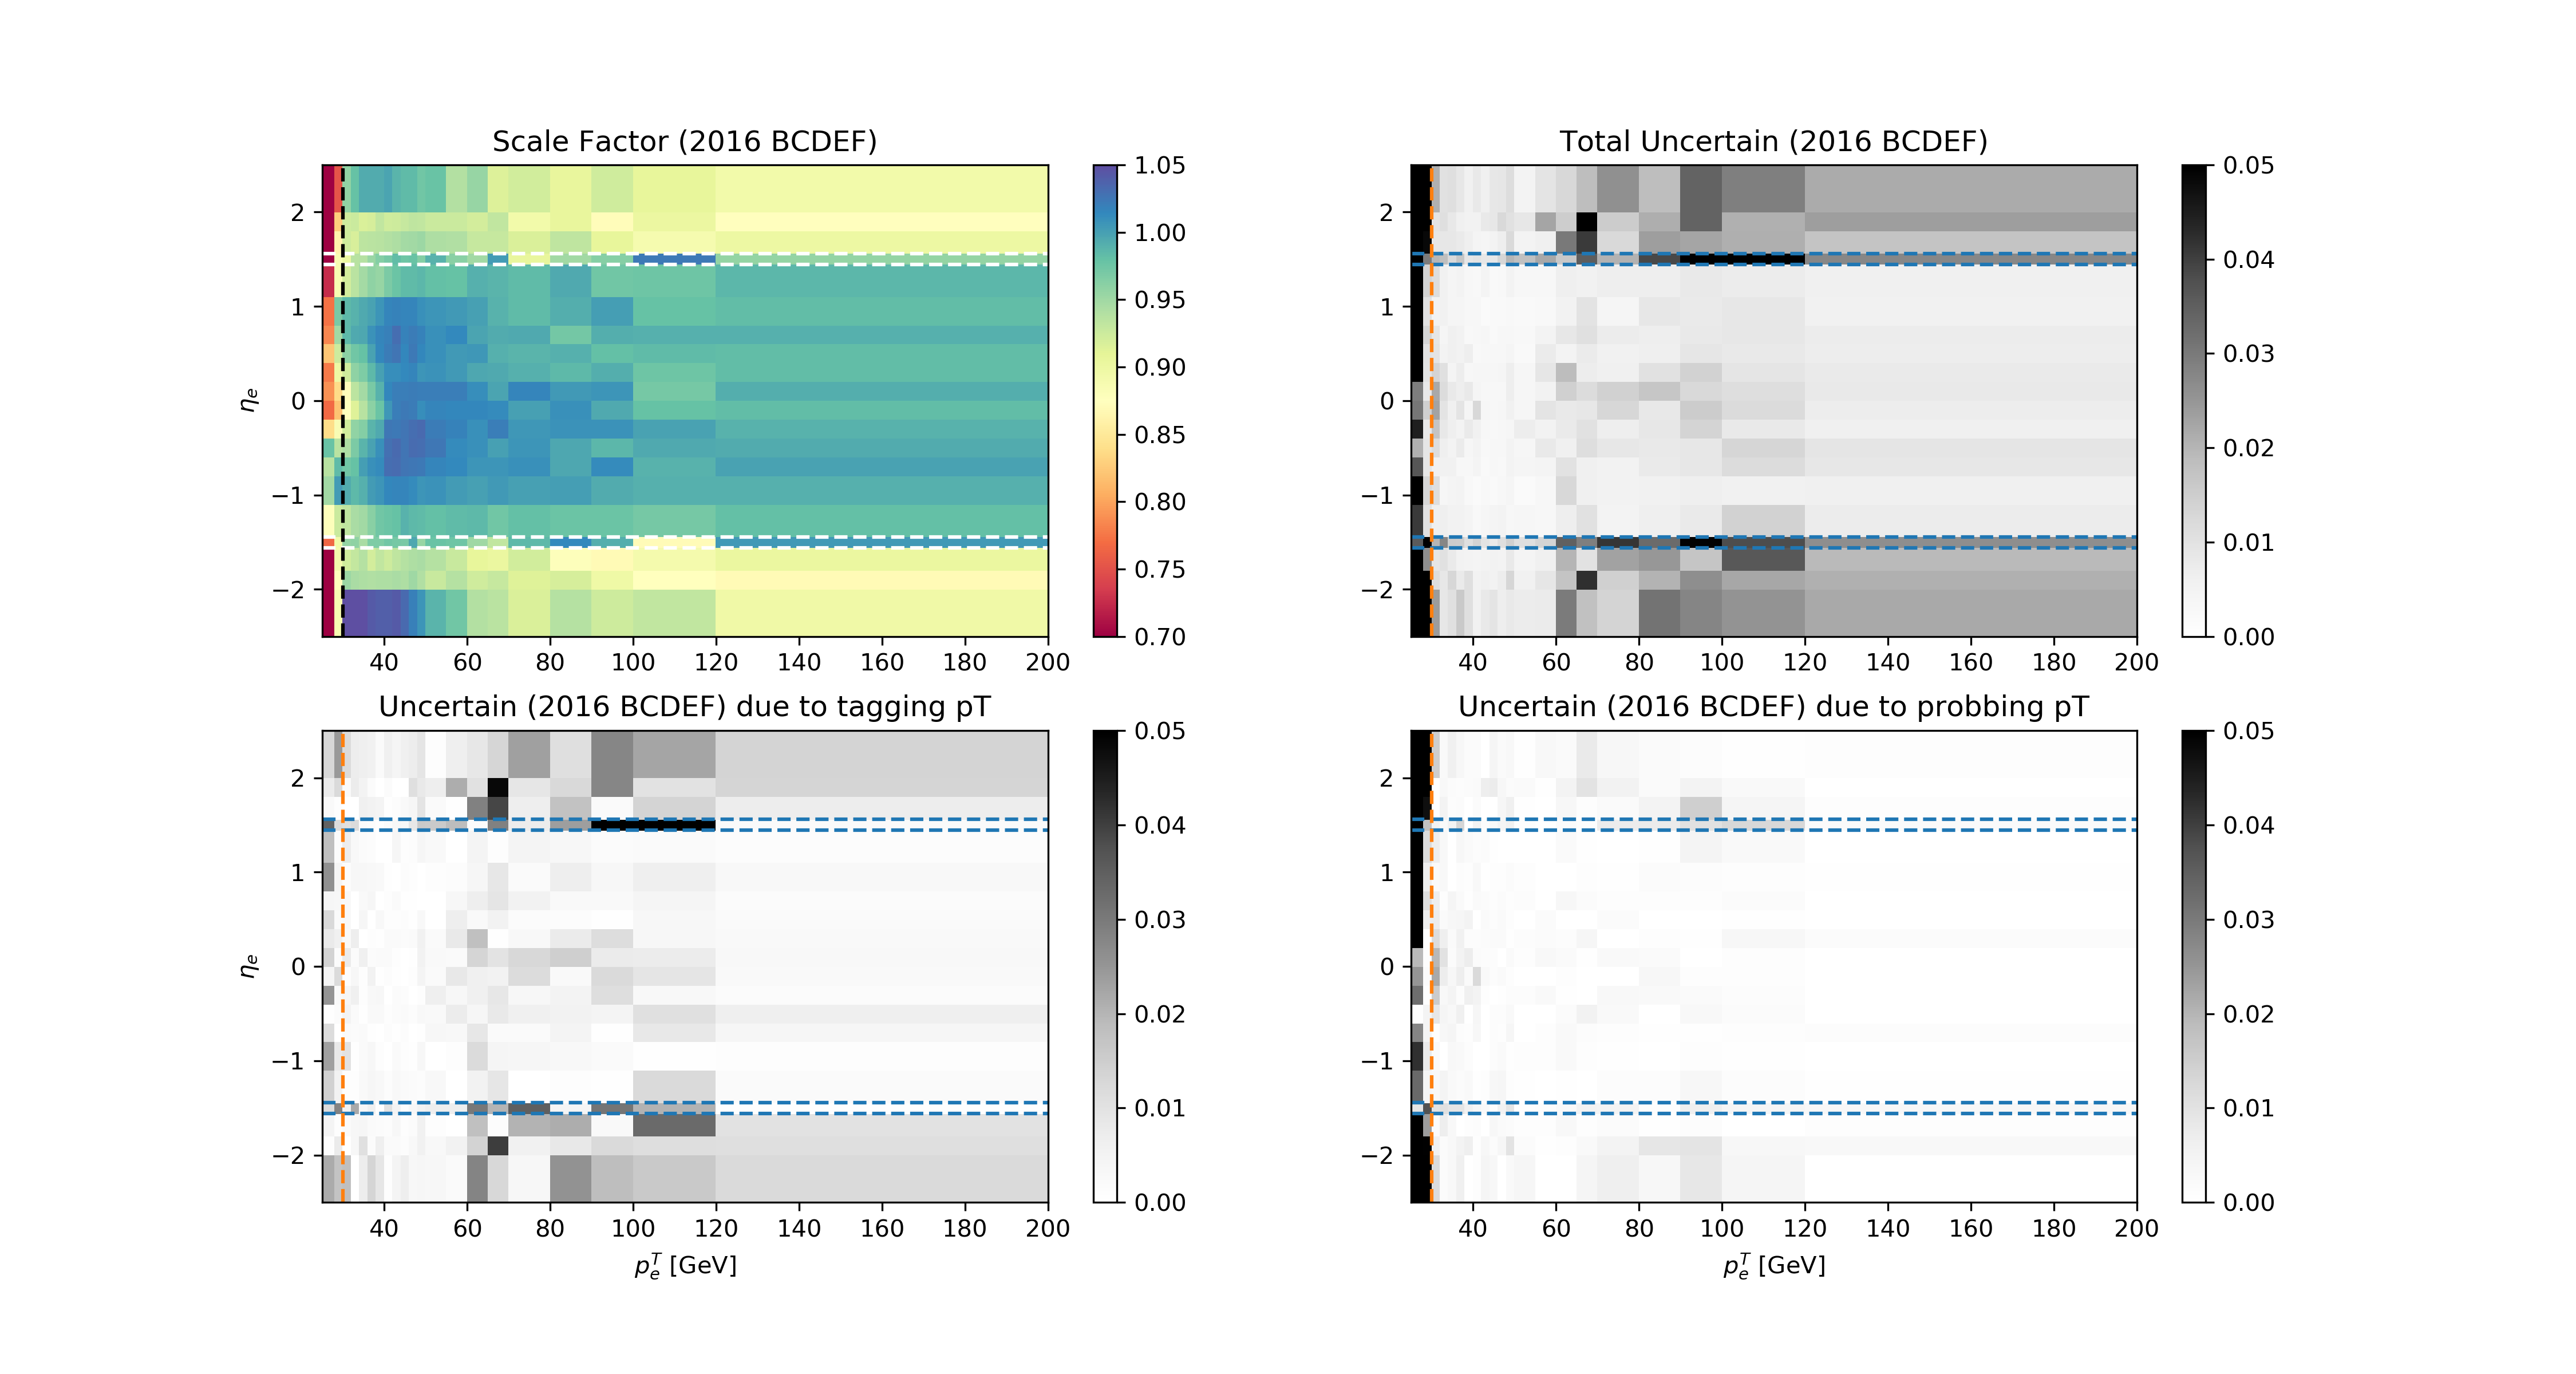
\includegraphics[width=0.99\textwidth]{chapters/Analysis/sectionCalibration/figures/eTrigger/result_BCDEF.png}
    \caption{SF and the associated uncertainties in the 2016 B-F.}
    \label{fig:eTrSF_err_BCDEF}
\end{figure}

\begin{figure}
    \centering
    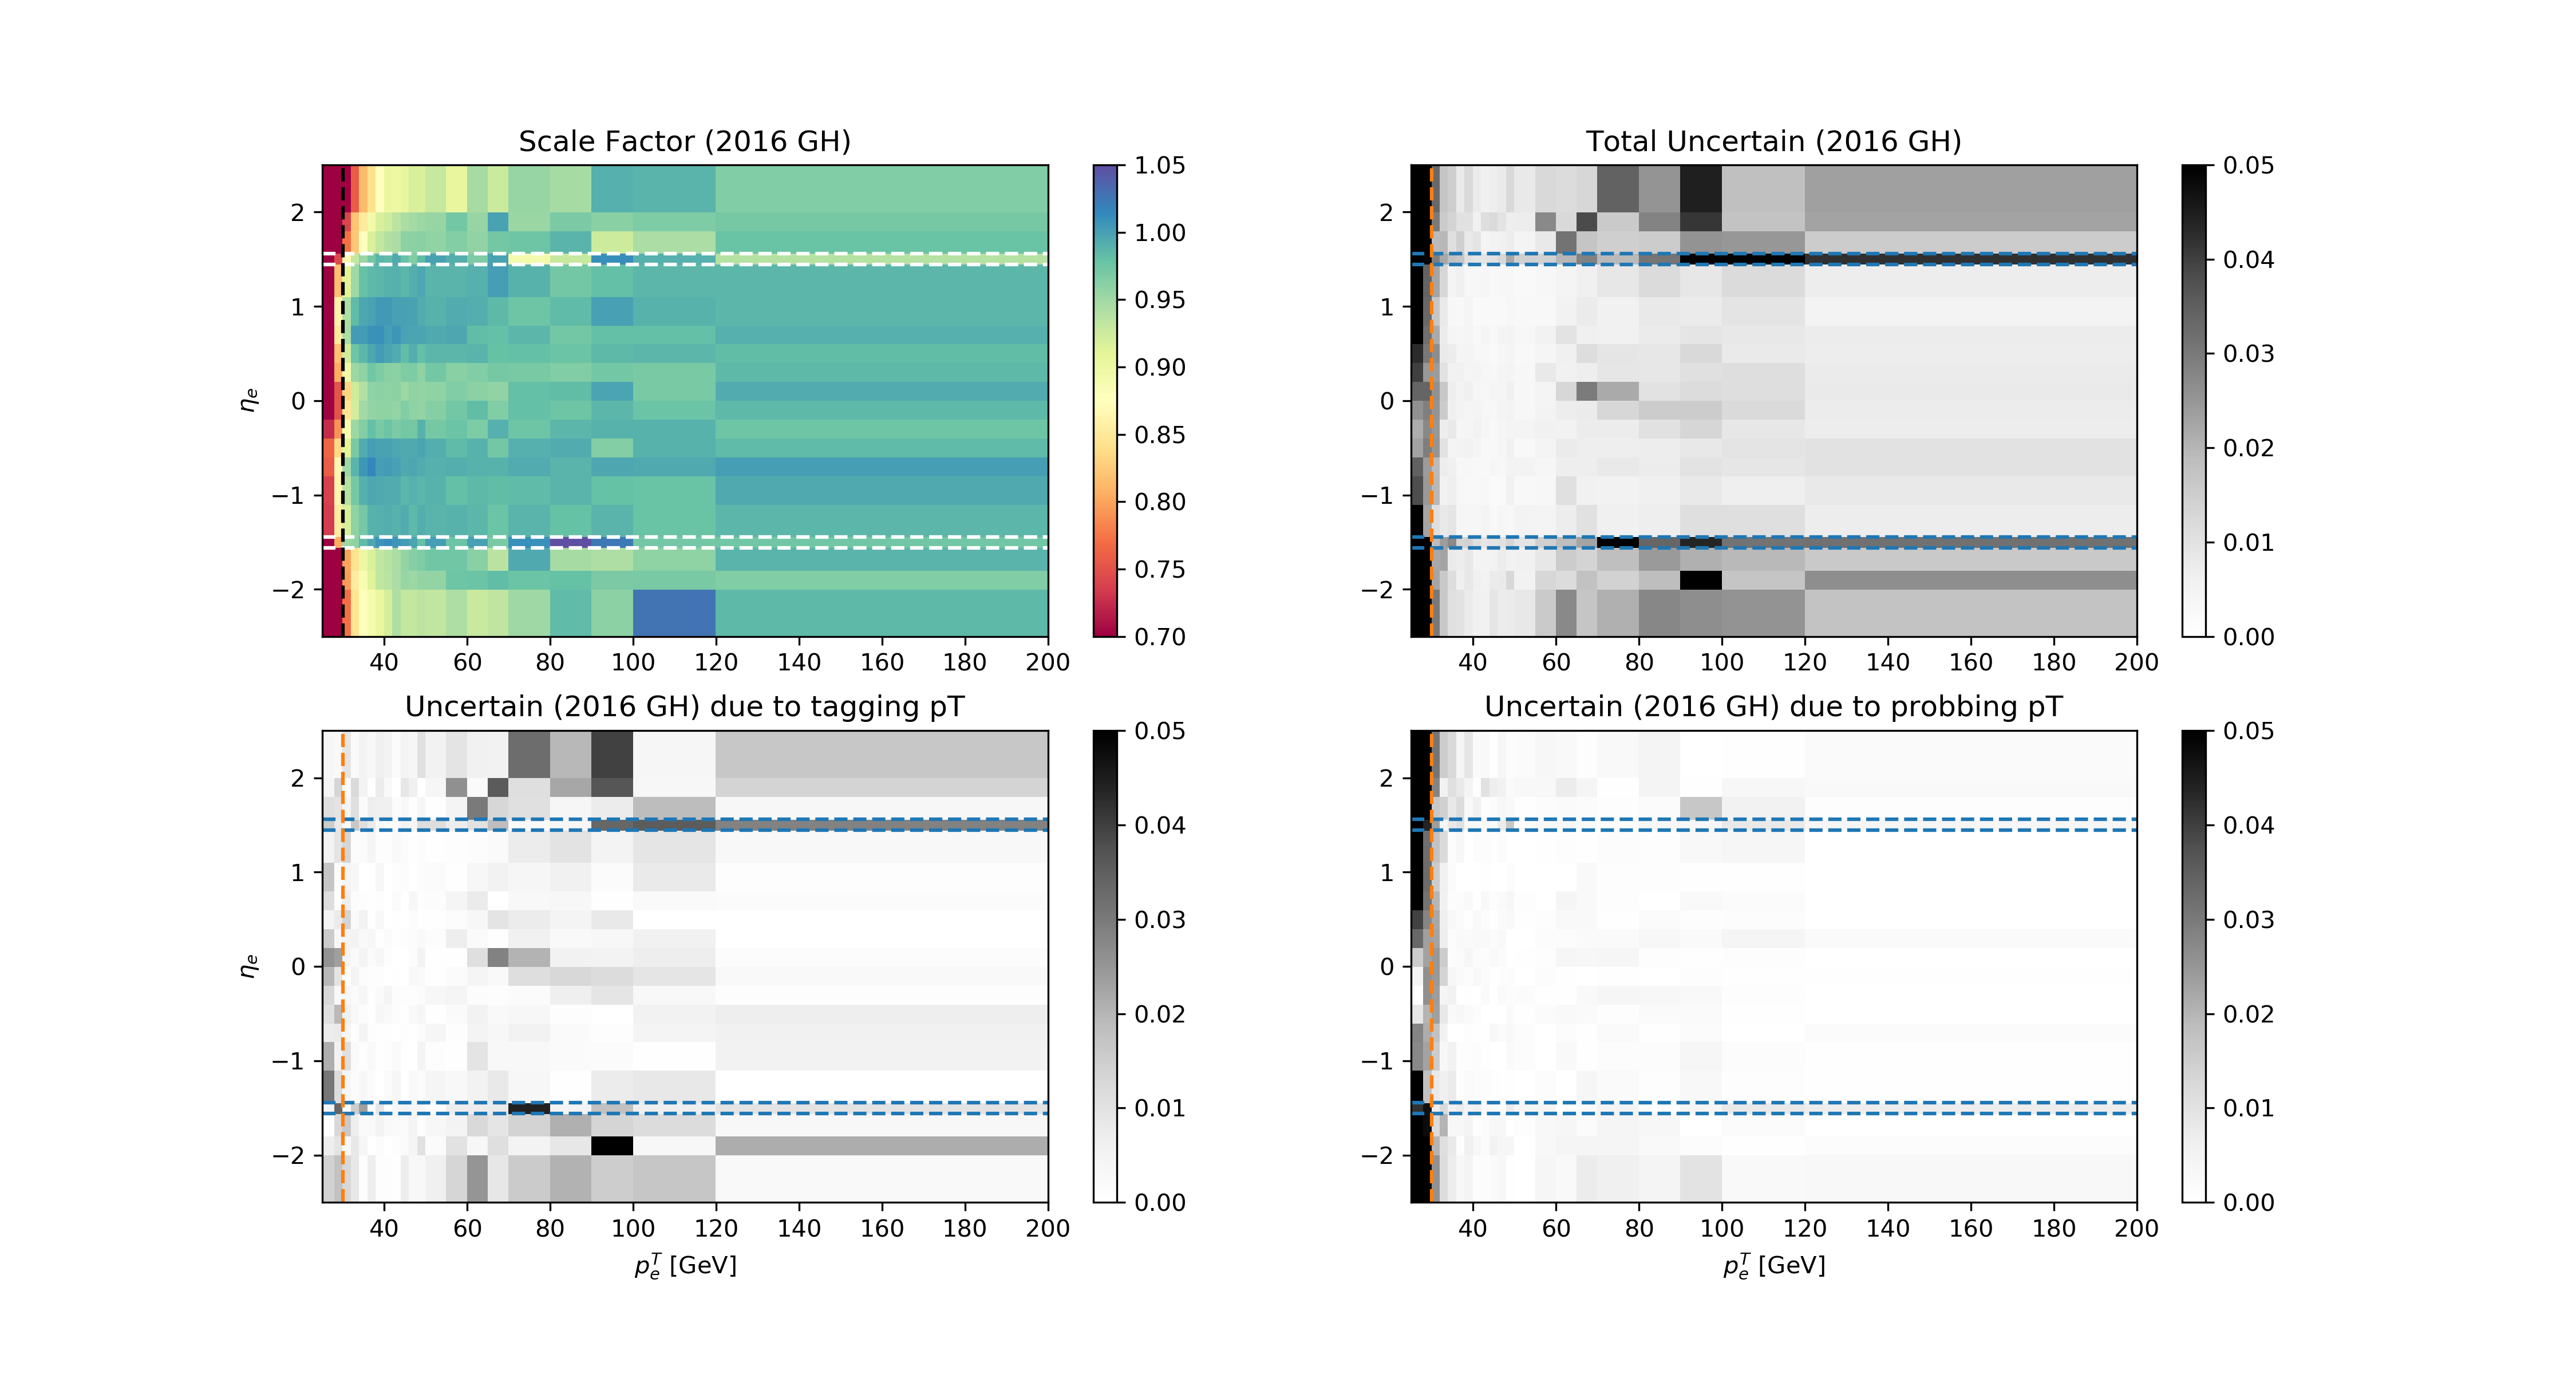
\includegraphics[width=0.99\textwidth]{chapters/Analysis/sectionCalibration/figures/eTrigger/result_GH.png}
    \caption{SF and the associated uncertainties in the 2016 GH.}
    \label{fig:eTrSF_err_GH}
\end{figure}

\FloatBarrier




\subsection{Measurement of Scale Factors for Jet Faking Hadronic Tau}
\label{sec:analysis:calibration:jetToTauh}


% \subsection{Measurement Approach}
In both the signal region and control region, $\mu \tau$ and $e \tau$ final states have sizable contributions from electron or muon plus a jet misidentified as a hadronic tau.  For correction to tau identification efficiency, tau POG has provided $SF (\tau_h \to \tau_h)$ measured with tag-prob technique at different identification working points.  However, regarding the $SF (j \to \tau_h)$, because the jet environment varies from analysis to analysis, tau POG suggests to measure it ourselves in a side-band region to correct $j \to \tau_h$ contributions and access corresponding uncertainties.

Our measurement of $SF (j\to \tau_h)$ is based on two regions, $t\bar{t}$ region which is enriched with b-jets identified as hadronic taus, $Z+jets$ region which is enriched with light jets identified as hadronic taus. Both Tight and VTight $\tau_h$ identification working points are considered.

\begin{itemize}
    \item $t\bar{t}$ region: $e\mu+\tau_h$ final state is selected. The selection requires exactly one muon and one electron with tight identification and isolation, plus one hadronic tau passing Tight or VTight working point. Corrections to reconstruction and selection of electron and muon are applied. The events has to fire either single muon trigger or single electron trigger.  The \pt threshold for triggering muon (electron) is 25 (30) GeV, while for non-triggering muon (electron) is 10 (20) GeV.  This selects a sample enriched with $t\bar{t}$ with $b \to \tau_h$. The kinematics of $e\mu+\tau$ final state events are shown in Figure~\ref{fig:appendix:fakeTauId:emutau}.
    
    
    \item $Z+jets$ region: $\mu\mu+\tau_h$ and $ee+\tau_h$ final state are selected.  The selection requires exactly two muons or two electrons with tight identification and isolation, plus one hadronic tau passing Tight or VTight working point.  Corrections to reconstruction and selection of electron and muon are applied. The trigger and \pt thresholds of leptons are the same as $e\mu+\tau_h$ final state.  This selects a sample enriched with $Z + jet$ with a light jet misidentified as $\tau_h$. The kinematics of $\mu\mu+\tau$ and $ee+\tau$ final states are shown in Figure~\ref{fig:appendix:fakeTauId:mumutau} and \ref{fig:appendix:fakeTauId:eetau}.
\end{itemize}

\noindent Note that the selections of $e\mu+\tau$, $\mu\mu+\tau$, $ee+\tau$ are developed based on the $e\mu$, $\mu\mu$, $ee$ selection in the main Br analysis,
using the same dilepton selection but requiring one additional Tight or VTight $\tau_h$. The origins of selected $\tau_h$ are tagged based on MC truth.  For each selected $\tau_h$, if there is a gen-level $\tau_h$ found within $\delta R = 0.3$, the $\tau_h$ is tagged as true identification.  If not a true identification, we try to match it with jet in the vetoed-jet collection and tag it as $j \to \tau_h$, flavor of which equals to the MC flavor of the jet correspondence.  In the rare cases where multiple jet correspondences are found, the one with highest pT is considered.  If neither gen-level $\tau_h$ match nor jet correspondence are found, the $\tau_h$ is untagged, which mainly due to $e \to \tau_h$. The gen-level  origin of $\tau_h$ are included in Figure~\ref{fig:appendix:fakeTauId:emutau,fig:appendix:fakeTauId:mumutau,fig:appendix:fakeTauId:eetau}.


\begin{figure}
    \centering
    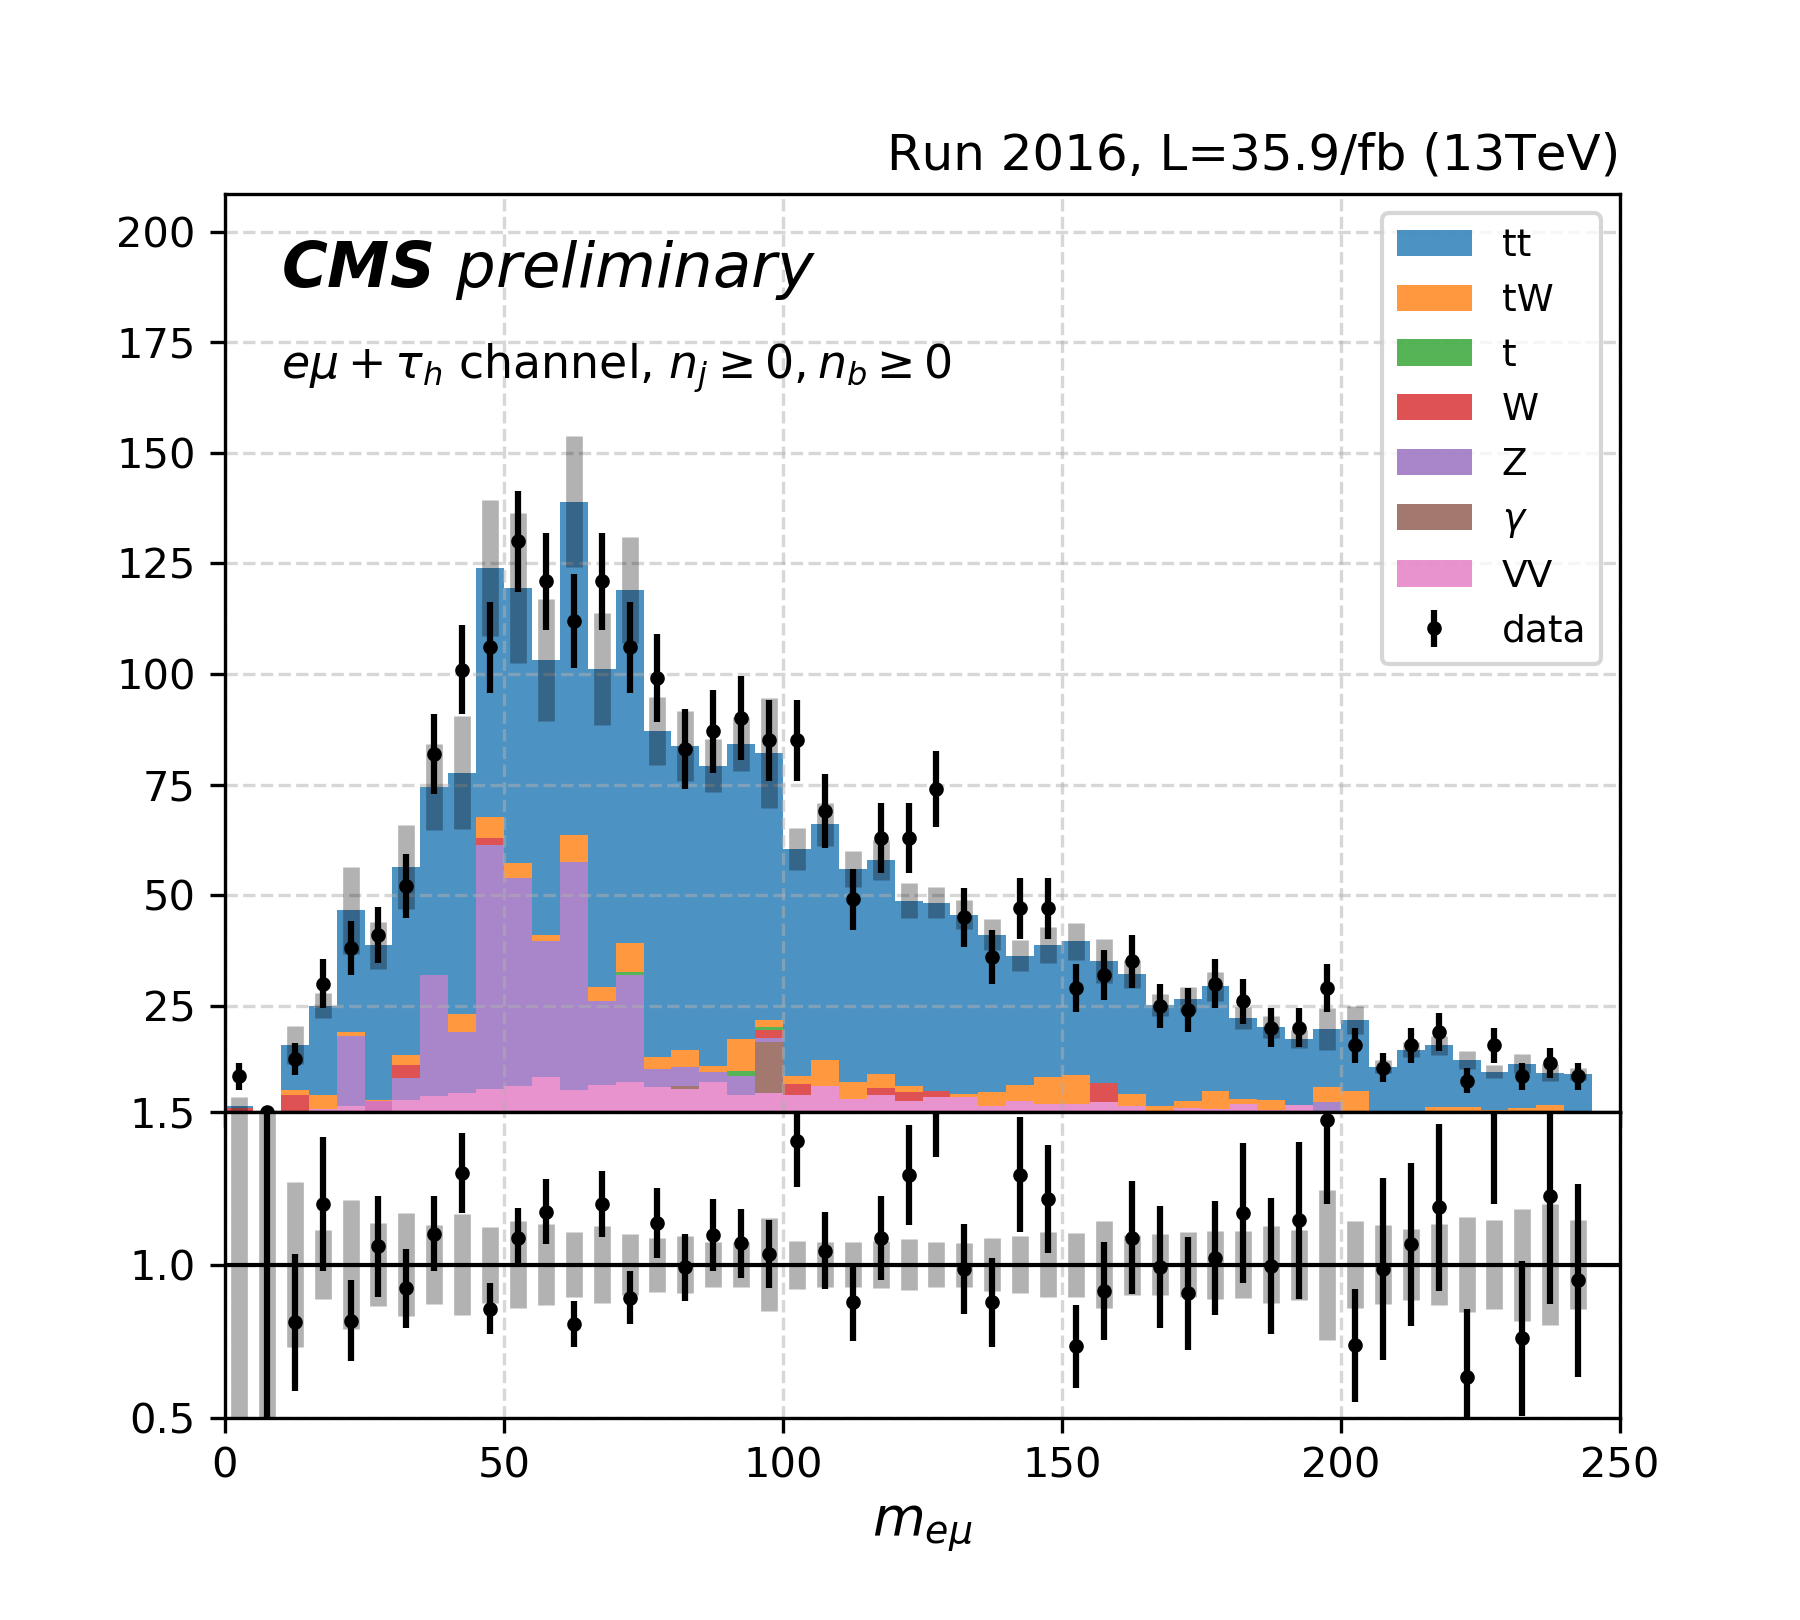
\includegraphics[width=0.4\textwidth]{chapters/Analysis/sectionCalibration/figures/jetToTauh/emutau_dilepton_mass_pickles_lltauTight.png}
    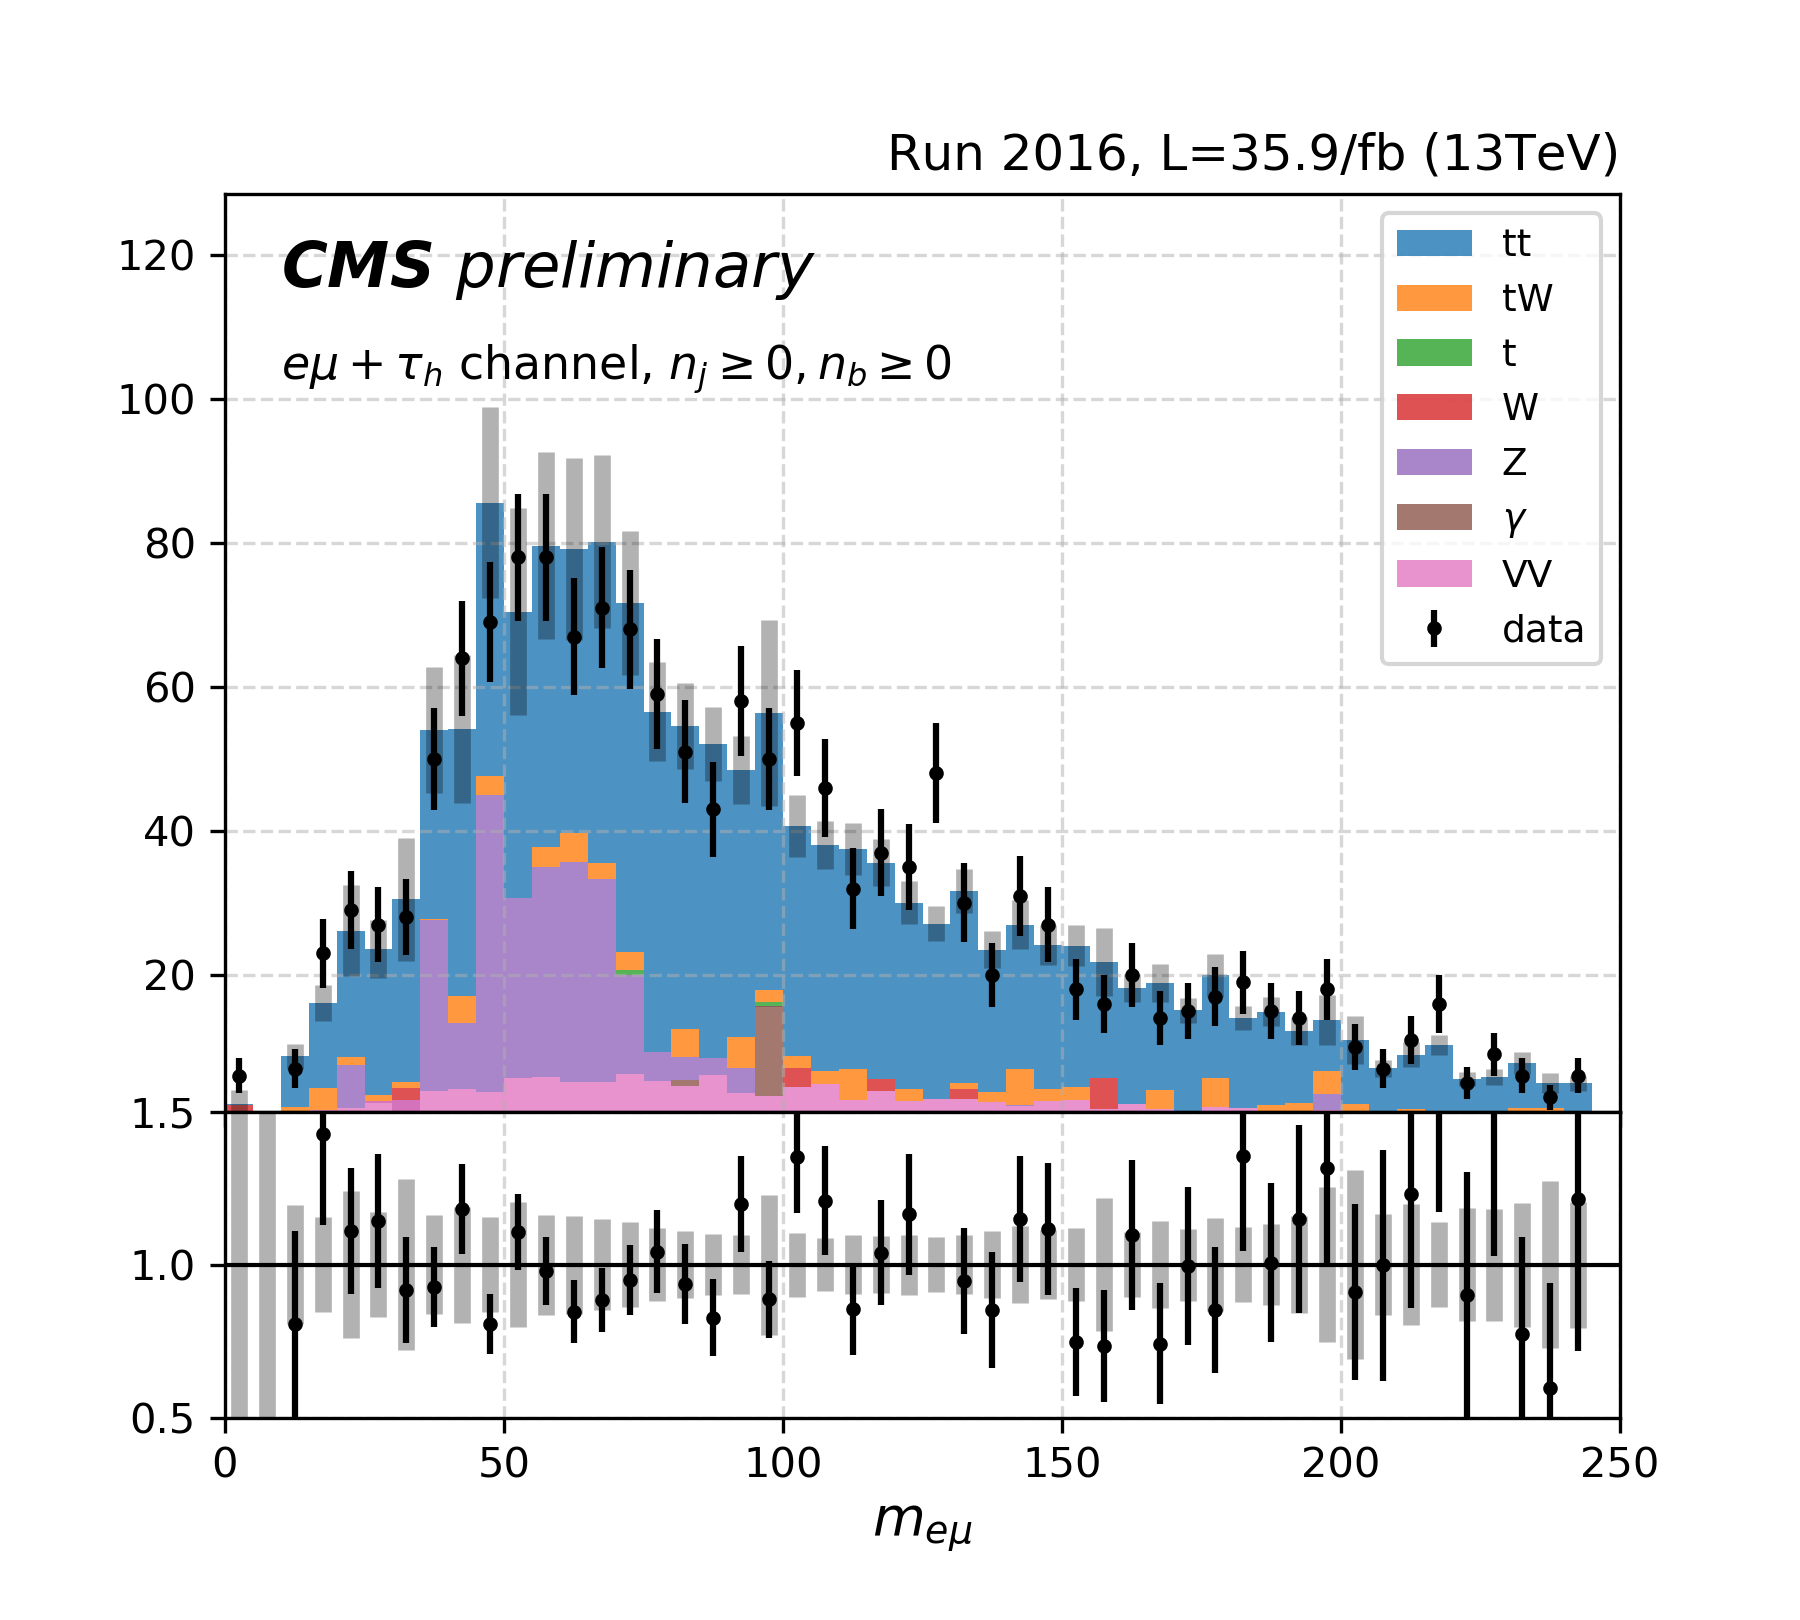
\includegraphics[width=0.4\textwidth]{chapters/Analysis/sectionCalibration/figures/jetToTauh/emutau_dilepton_mass_pickles_lltauVTight.png}
    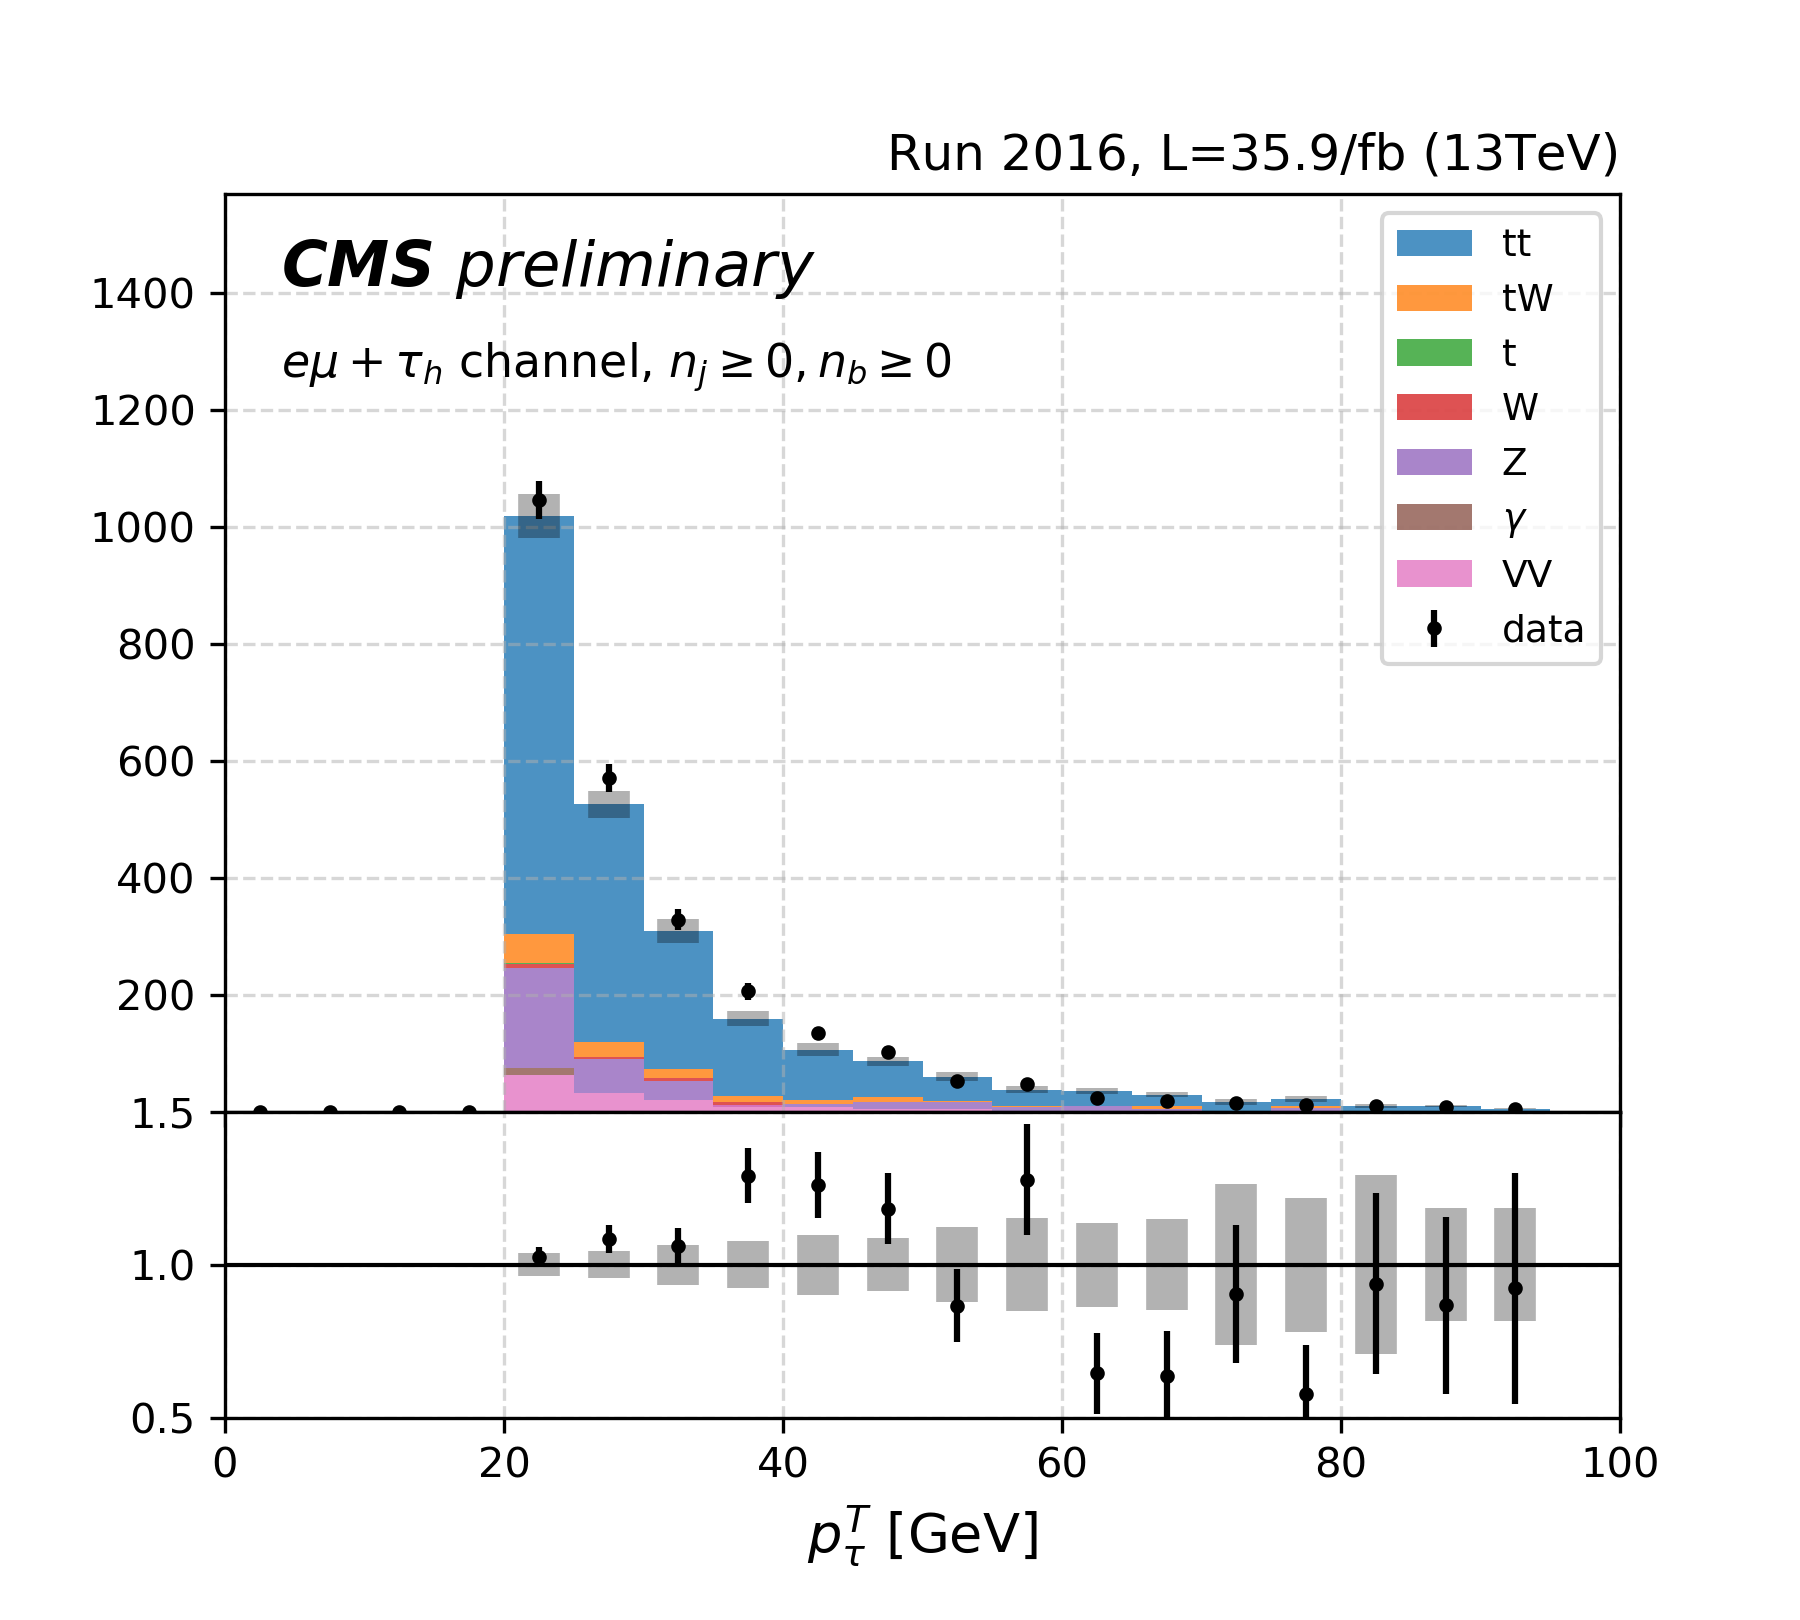
\includegraphics[width=0.4\textwidth]{chapters/Analysis/sectionCalibration/figures/jetToTauh/emutau_tauPt_pickles_lltauTight.png}
    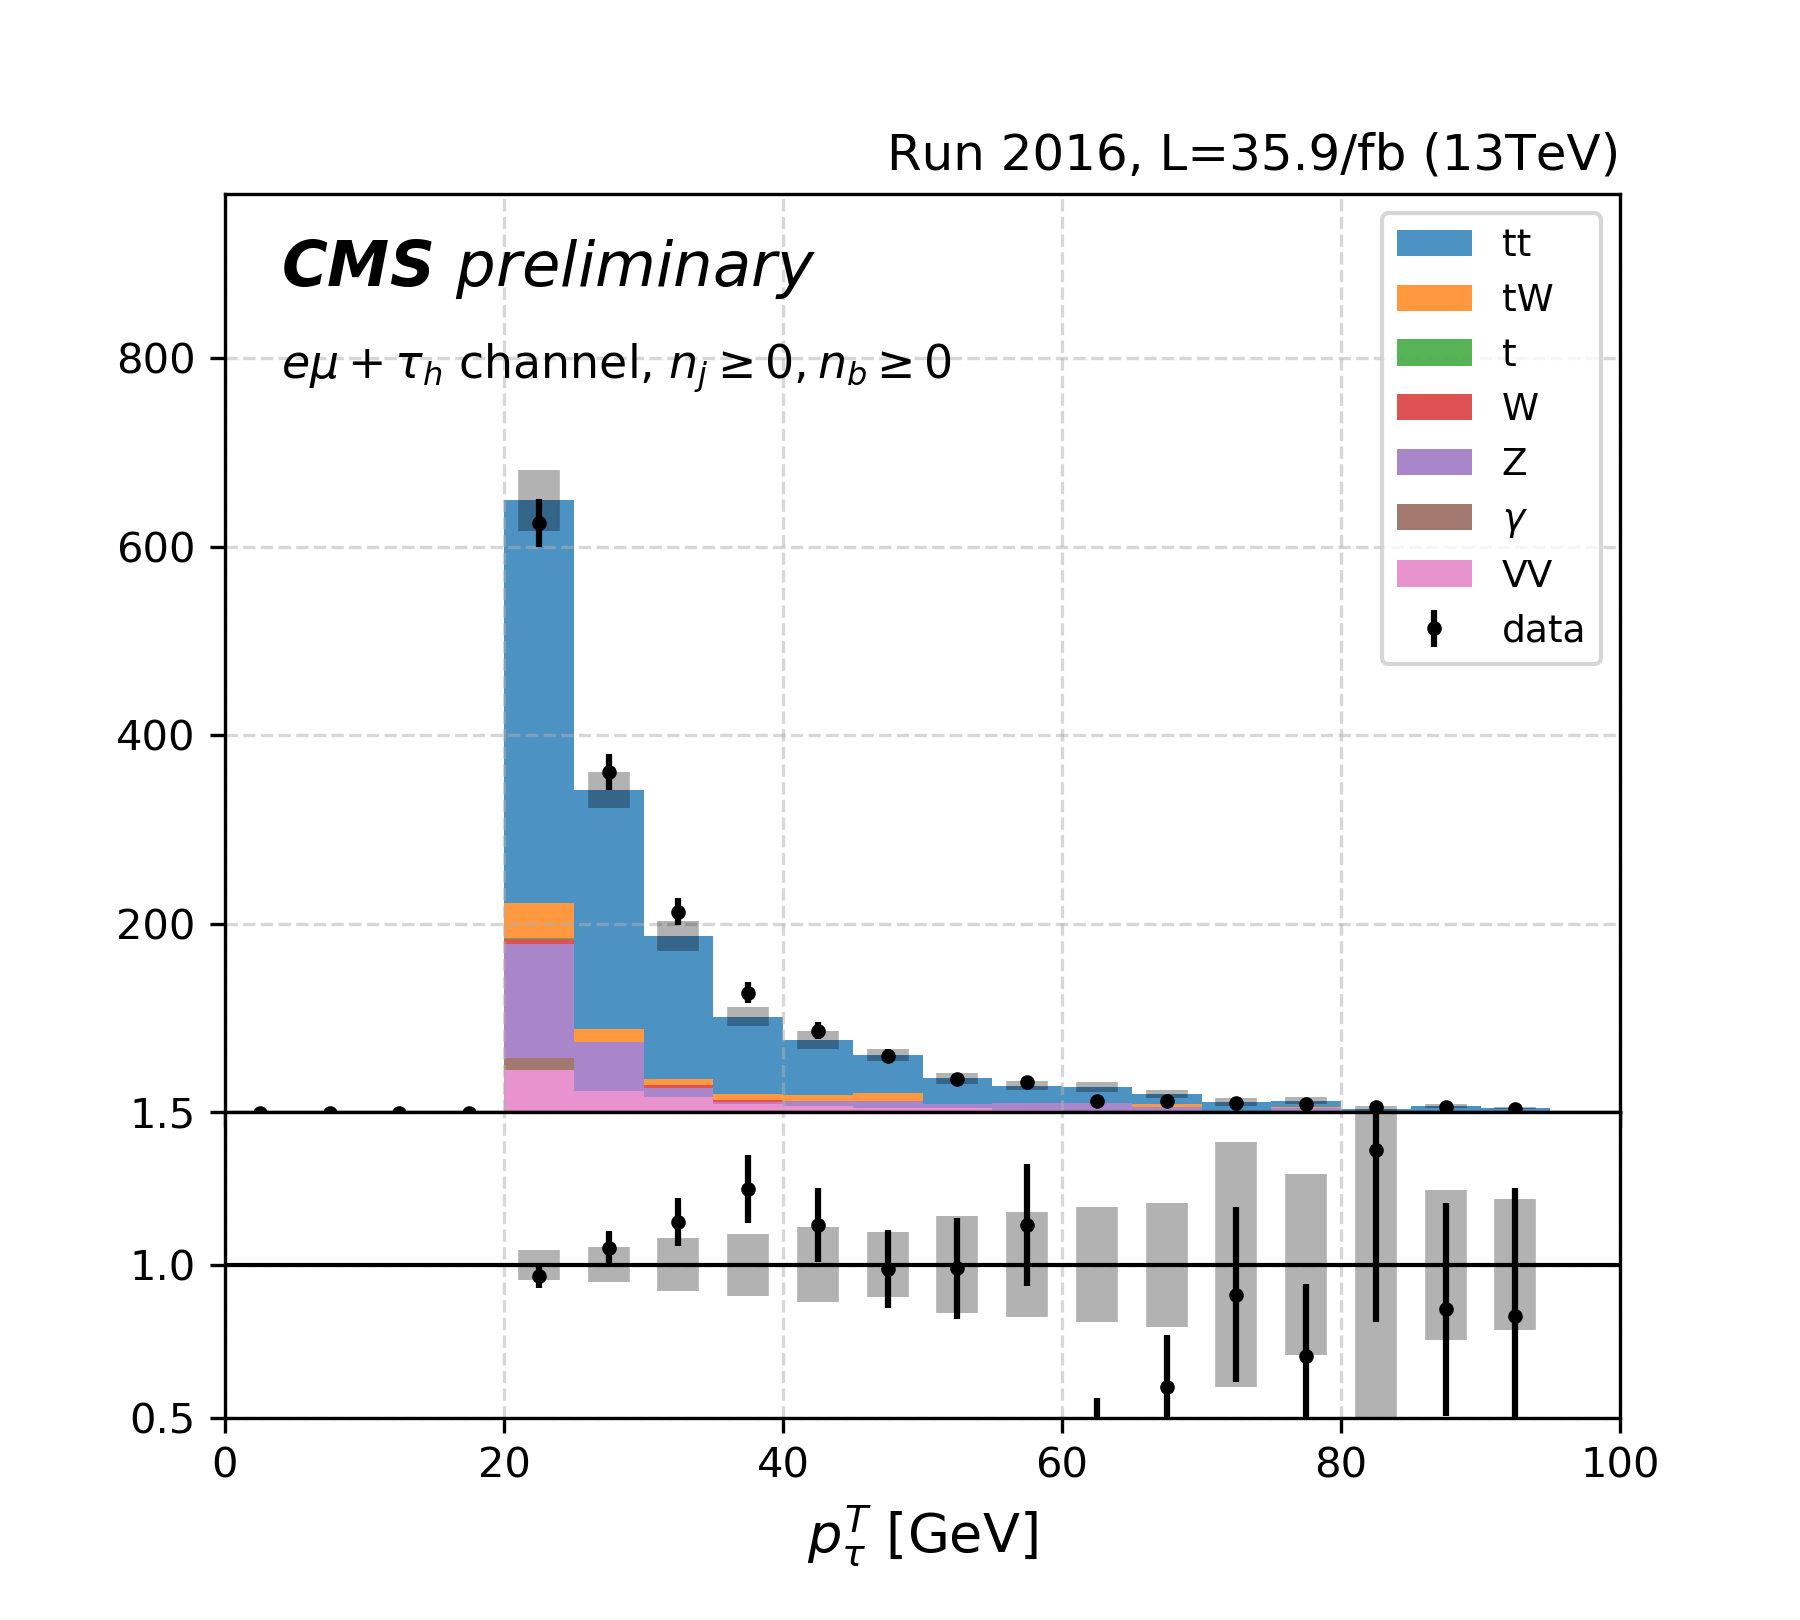
\includegraphics[width=0.4\textwidth]{chapters/Analysis/sectionCalibration/figures/jetToTauh/emutau_tauPt_pickles_lltauVTight.png}
    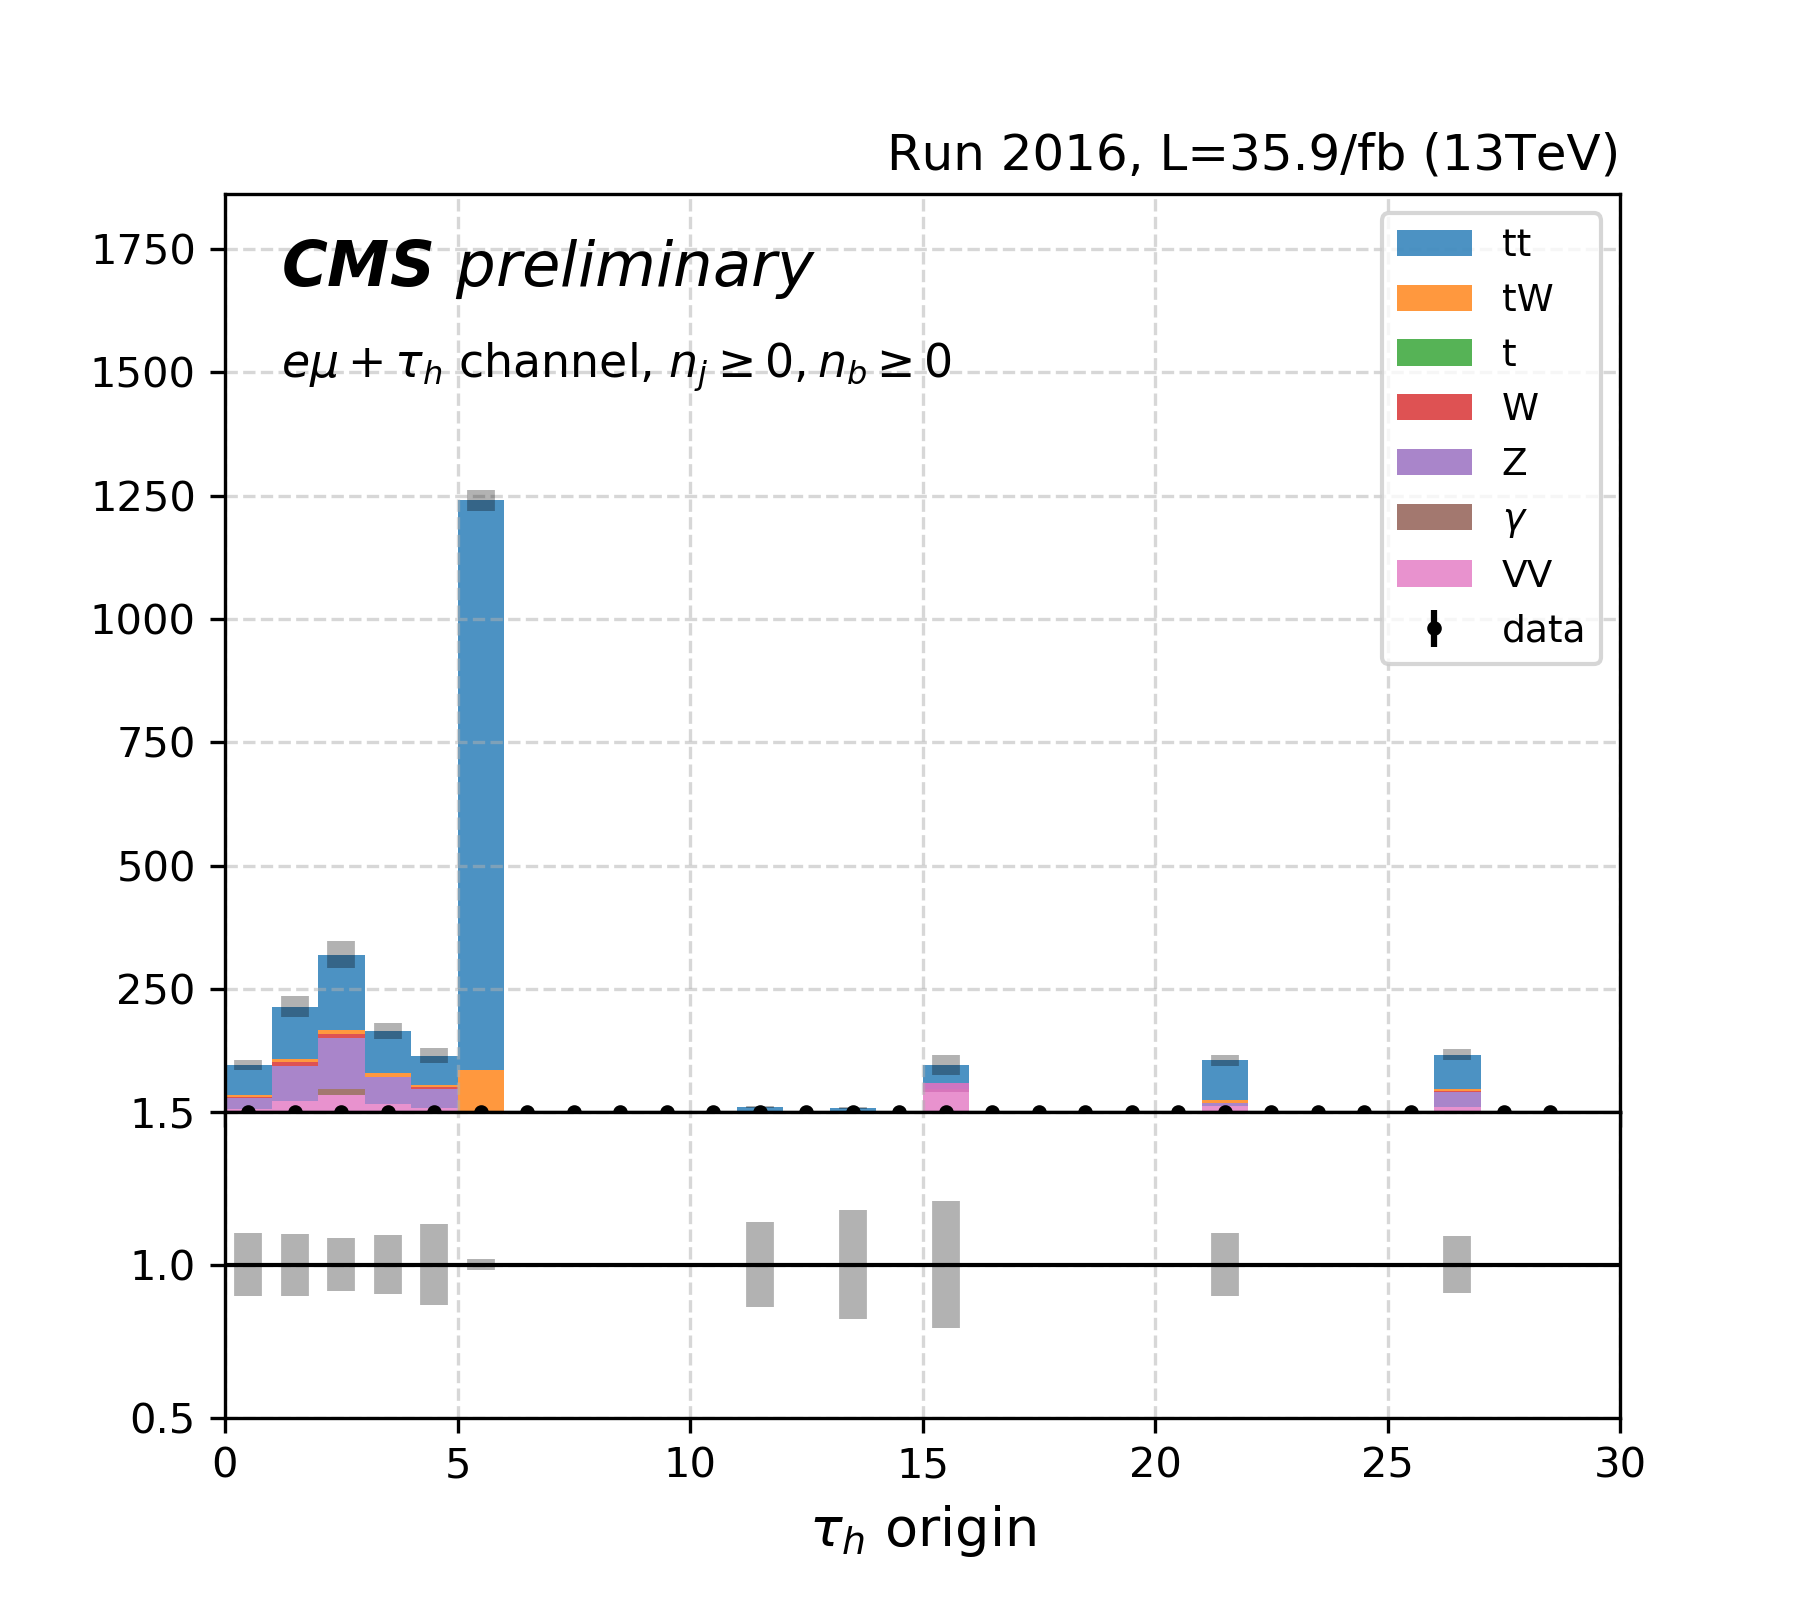
\includegraphics[width=0.4\textwidth]{chapters/Analysis/sectionCalibration/figures/jetToTauh/emutau_tauGenFlavor_pickles_lltauTight.png}
    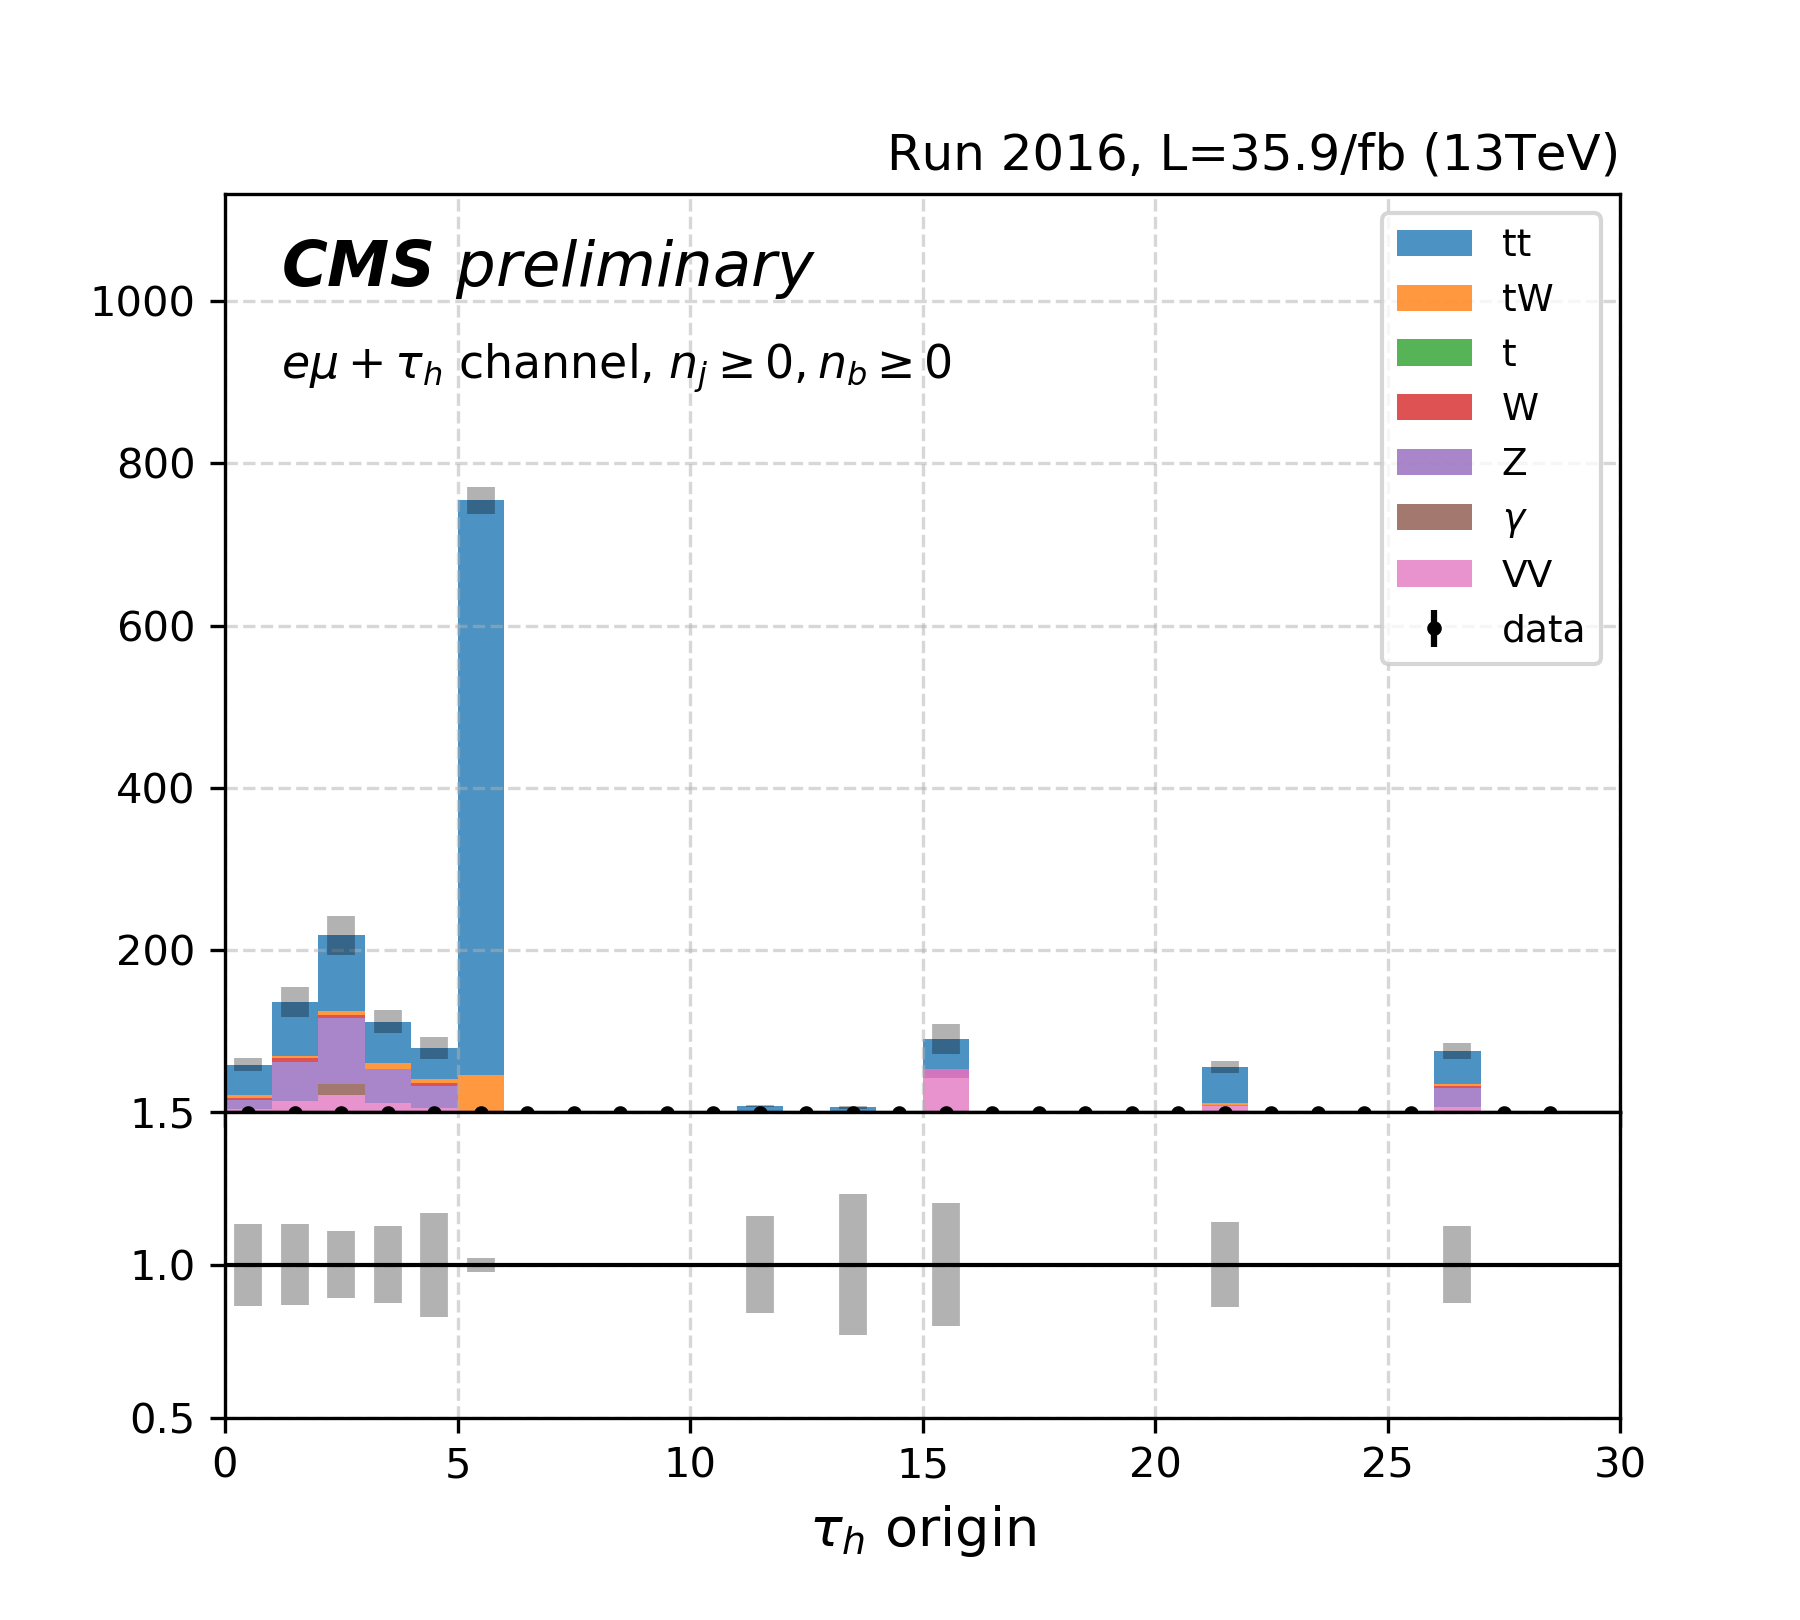
\includegraphics[width=0.4\textwidth]{chapters/Analysis/sectionCalibration/figures/jetToTauh/emutau_tauGenFlavor_pickles_lltauVTight.png}
    \caption{Distributions of $m_{e\mu}$, $\tau_h$ \pt and gen-level $\tau_h$ origin in the $e\mu+\tau$ channel. The left and right column shows the Tight and VTight $\tau_h$ WP respectively.}
    \label{fig:appendix:fakeTauId:emutau}
\end{figure}

\begin{figure}
    \centering
    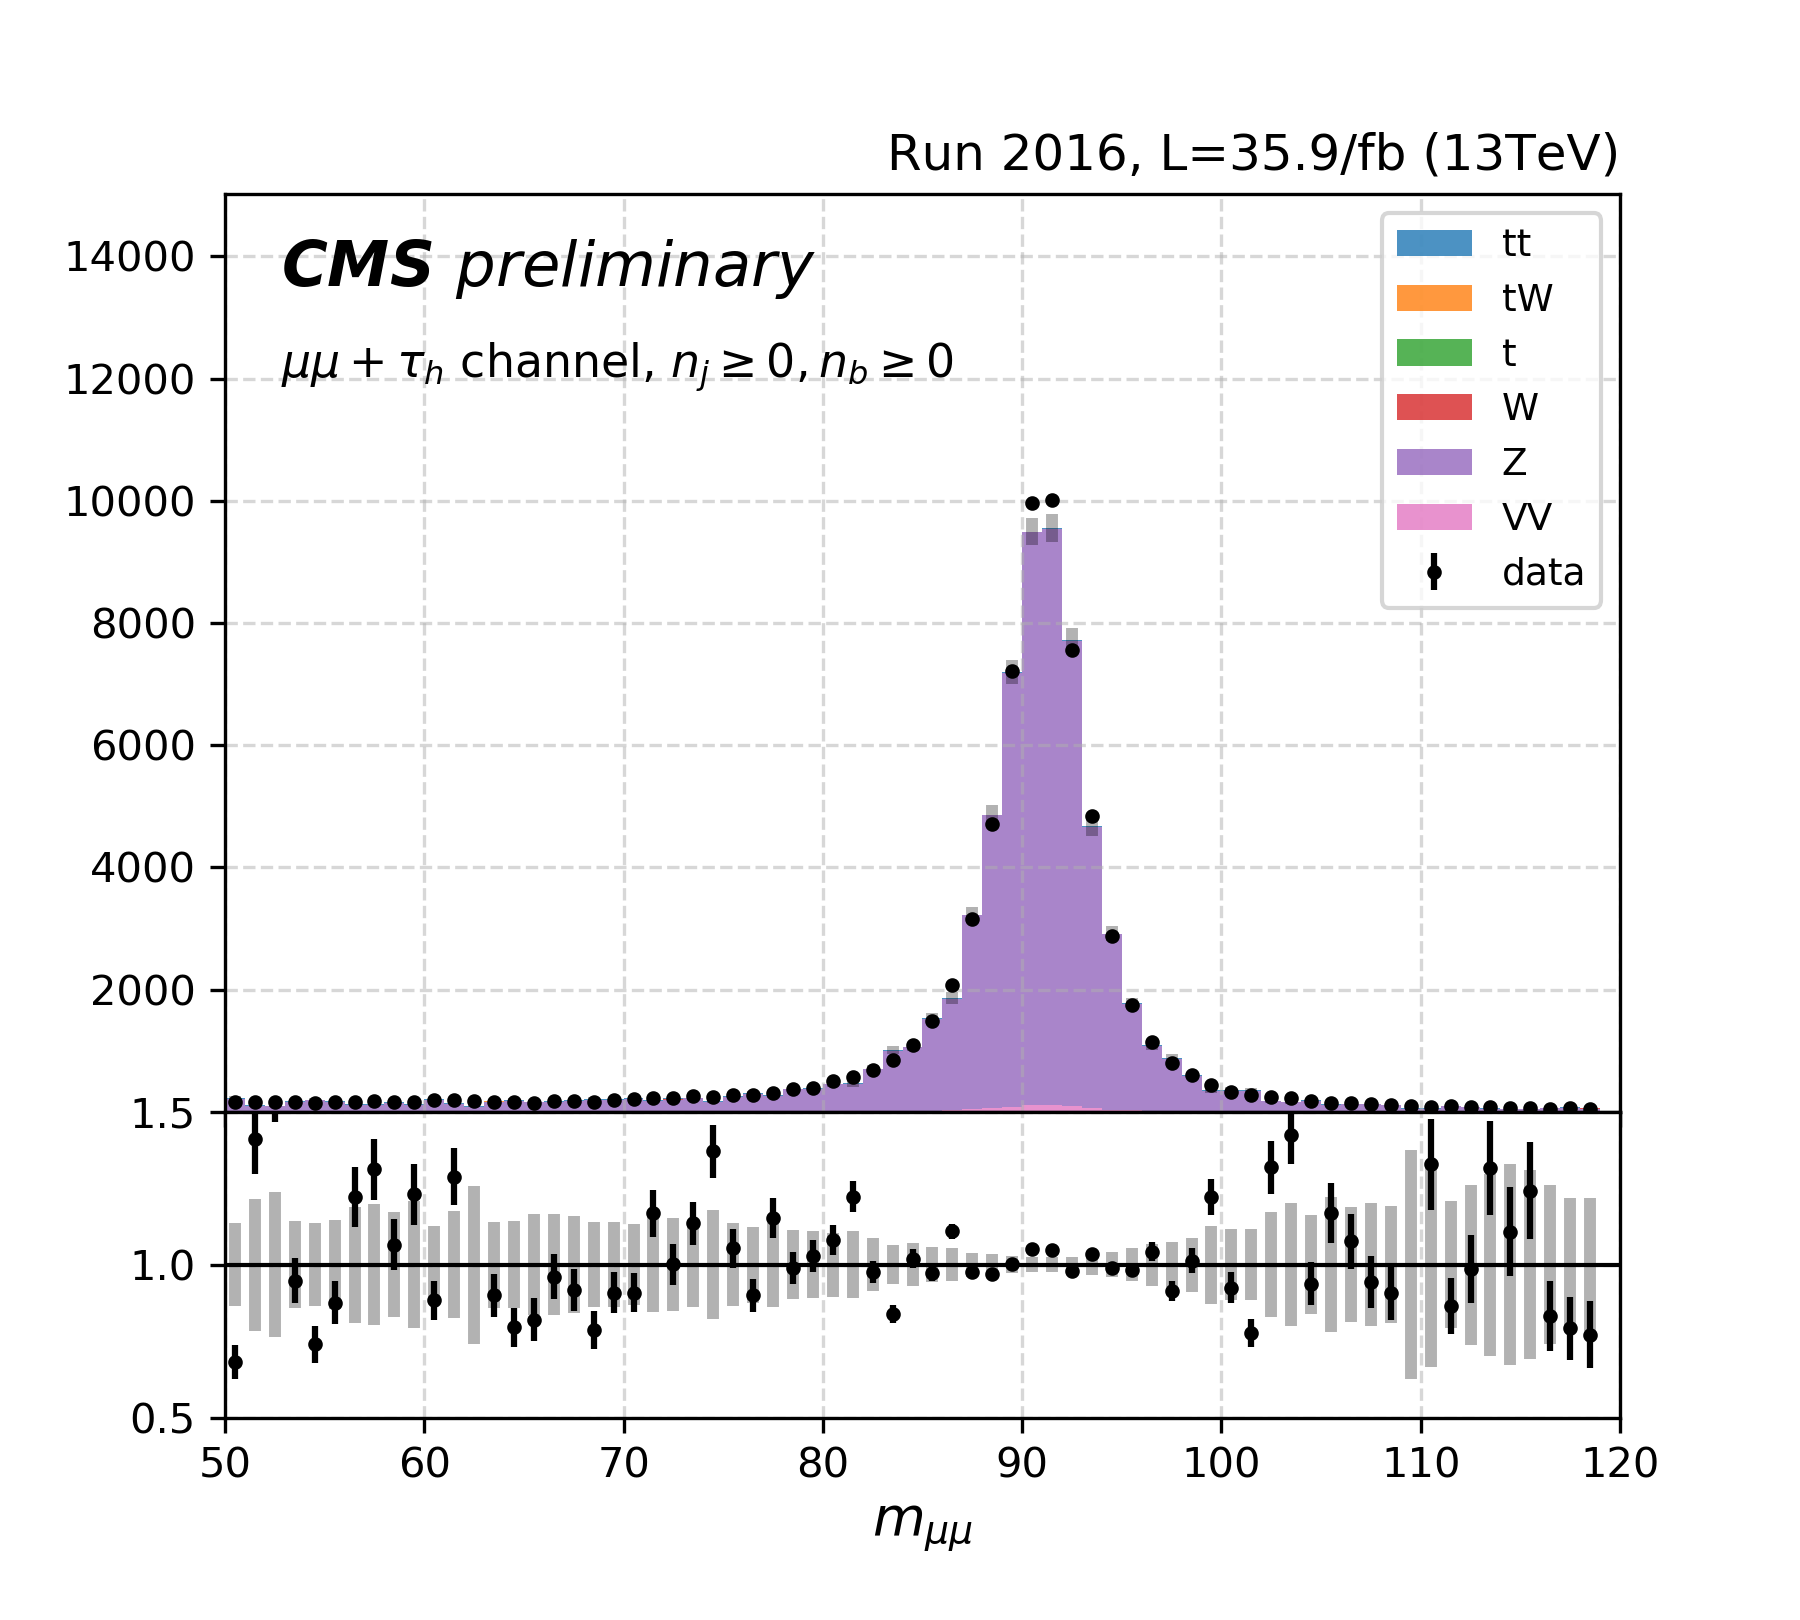
\includegraphics[width=0.4\textwidth]{chapters/Analysis/sectionCalibration/figures/jetToTauh/mumutau_dilepton_mass_pickles_lltauTight.png}
    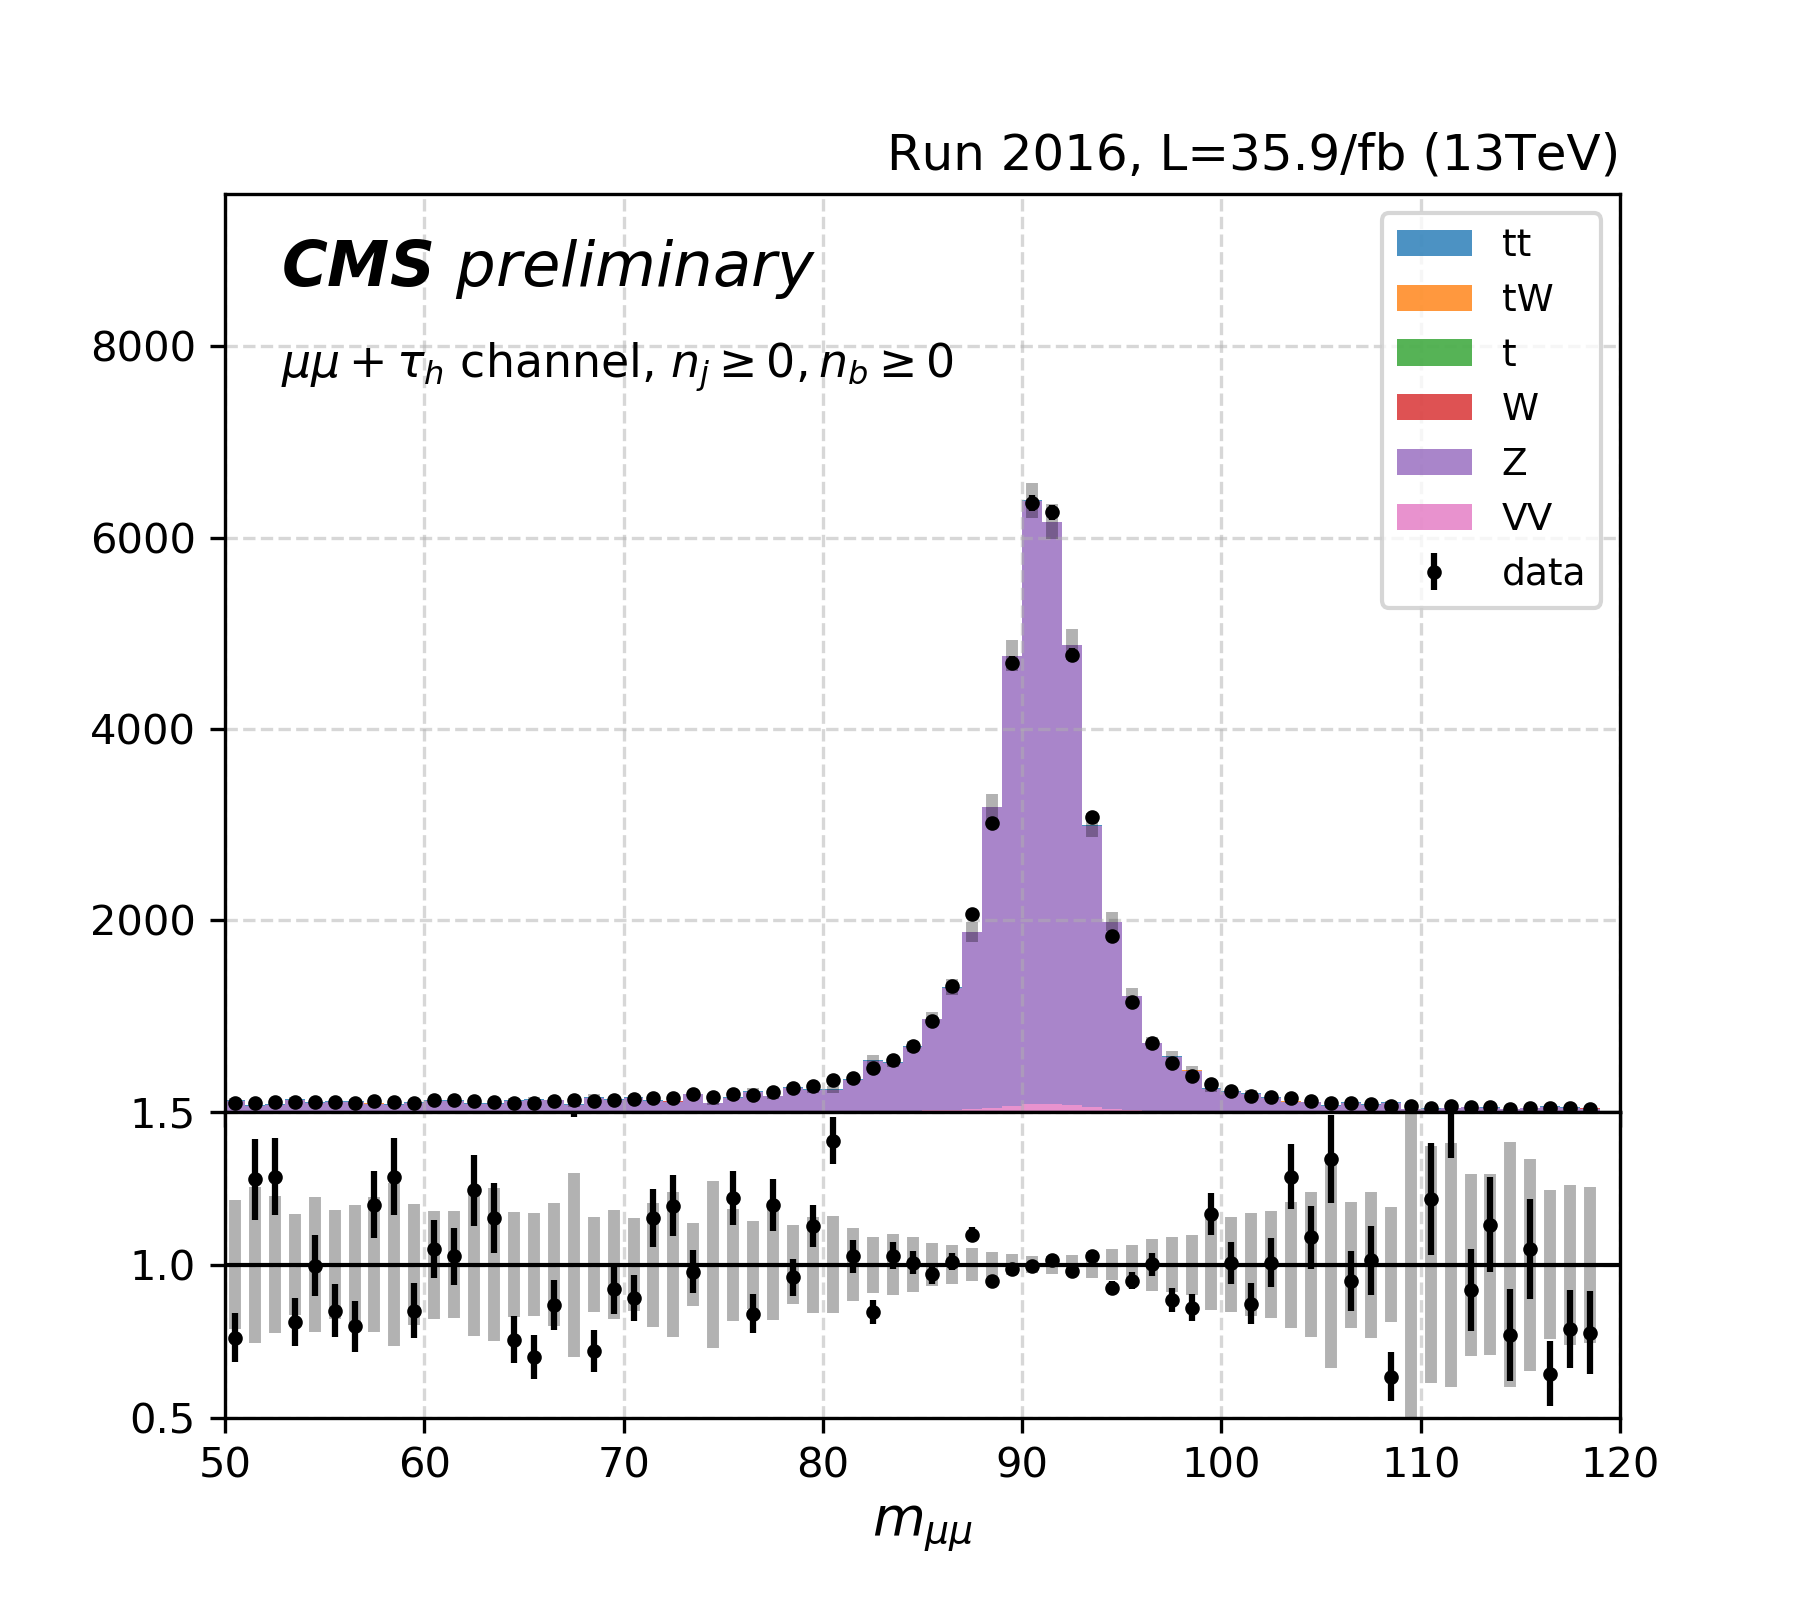
\includegraphics[width=0.4\textwidth]{chapters/Analysis/sectionCalibration/figures/jetToTauh/mumutau_dilepton_mass_pickles_lltauVTight.png}
    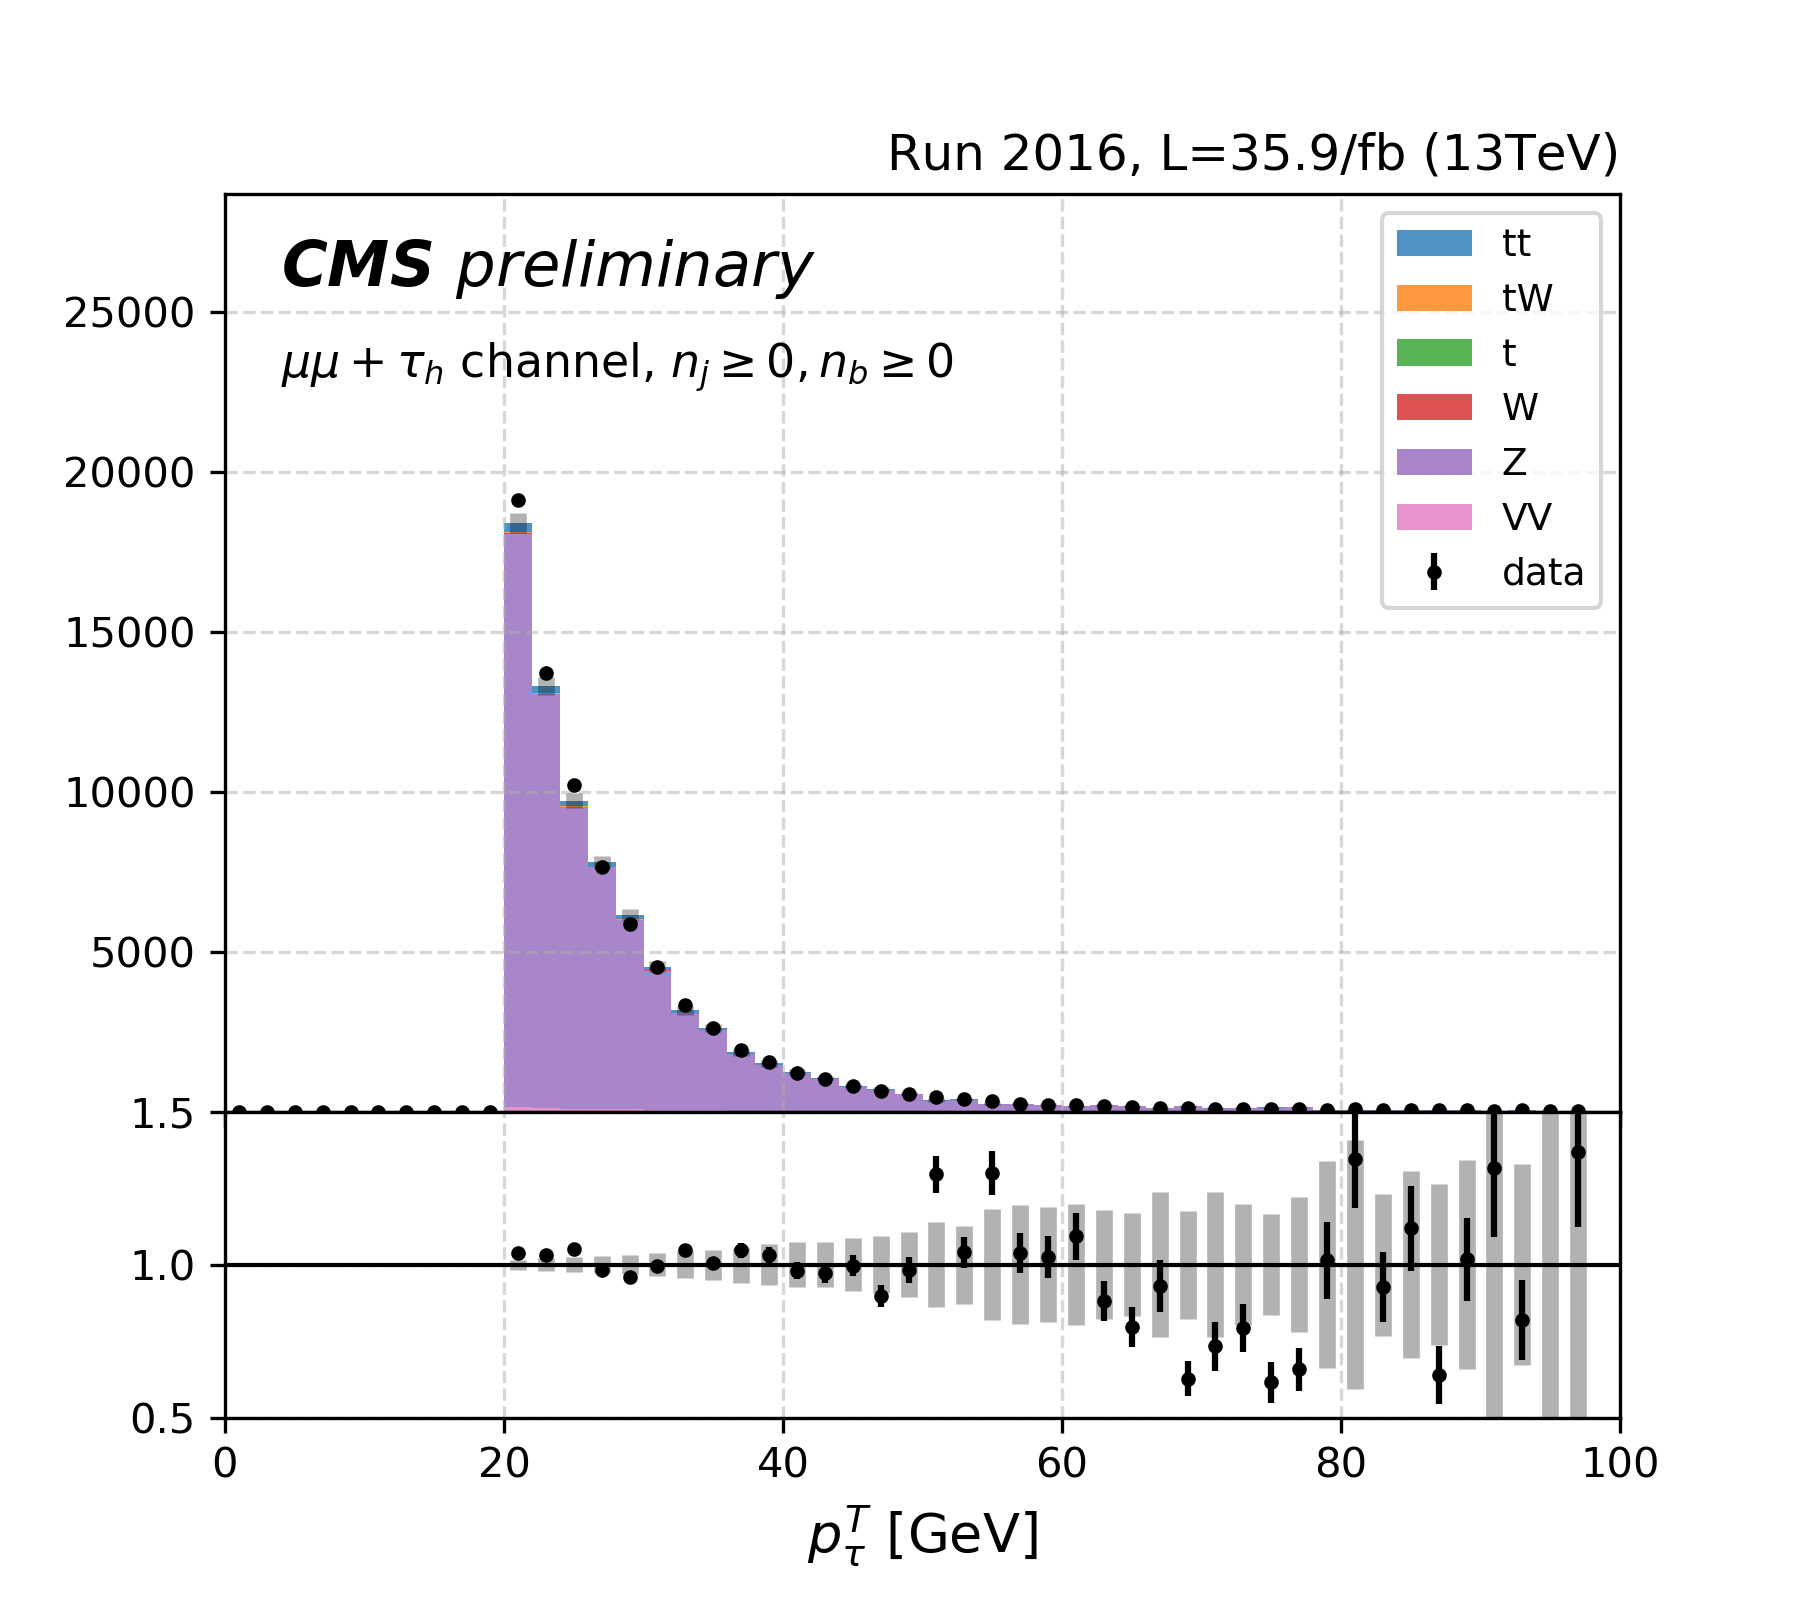
\includegraphics[width=0.4\textwidth]{chapters/Analysis/sectionCalibration/figures/jetToTauh/mumutau_tauPt_pickles_lltauTight.png}
    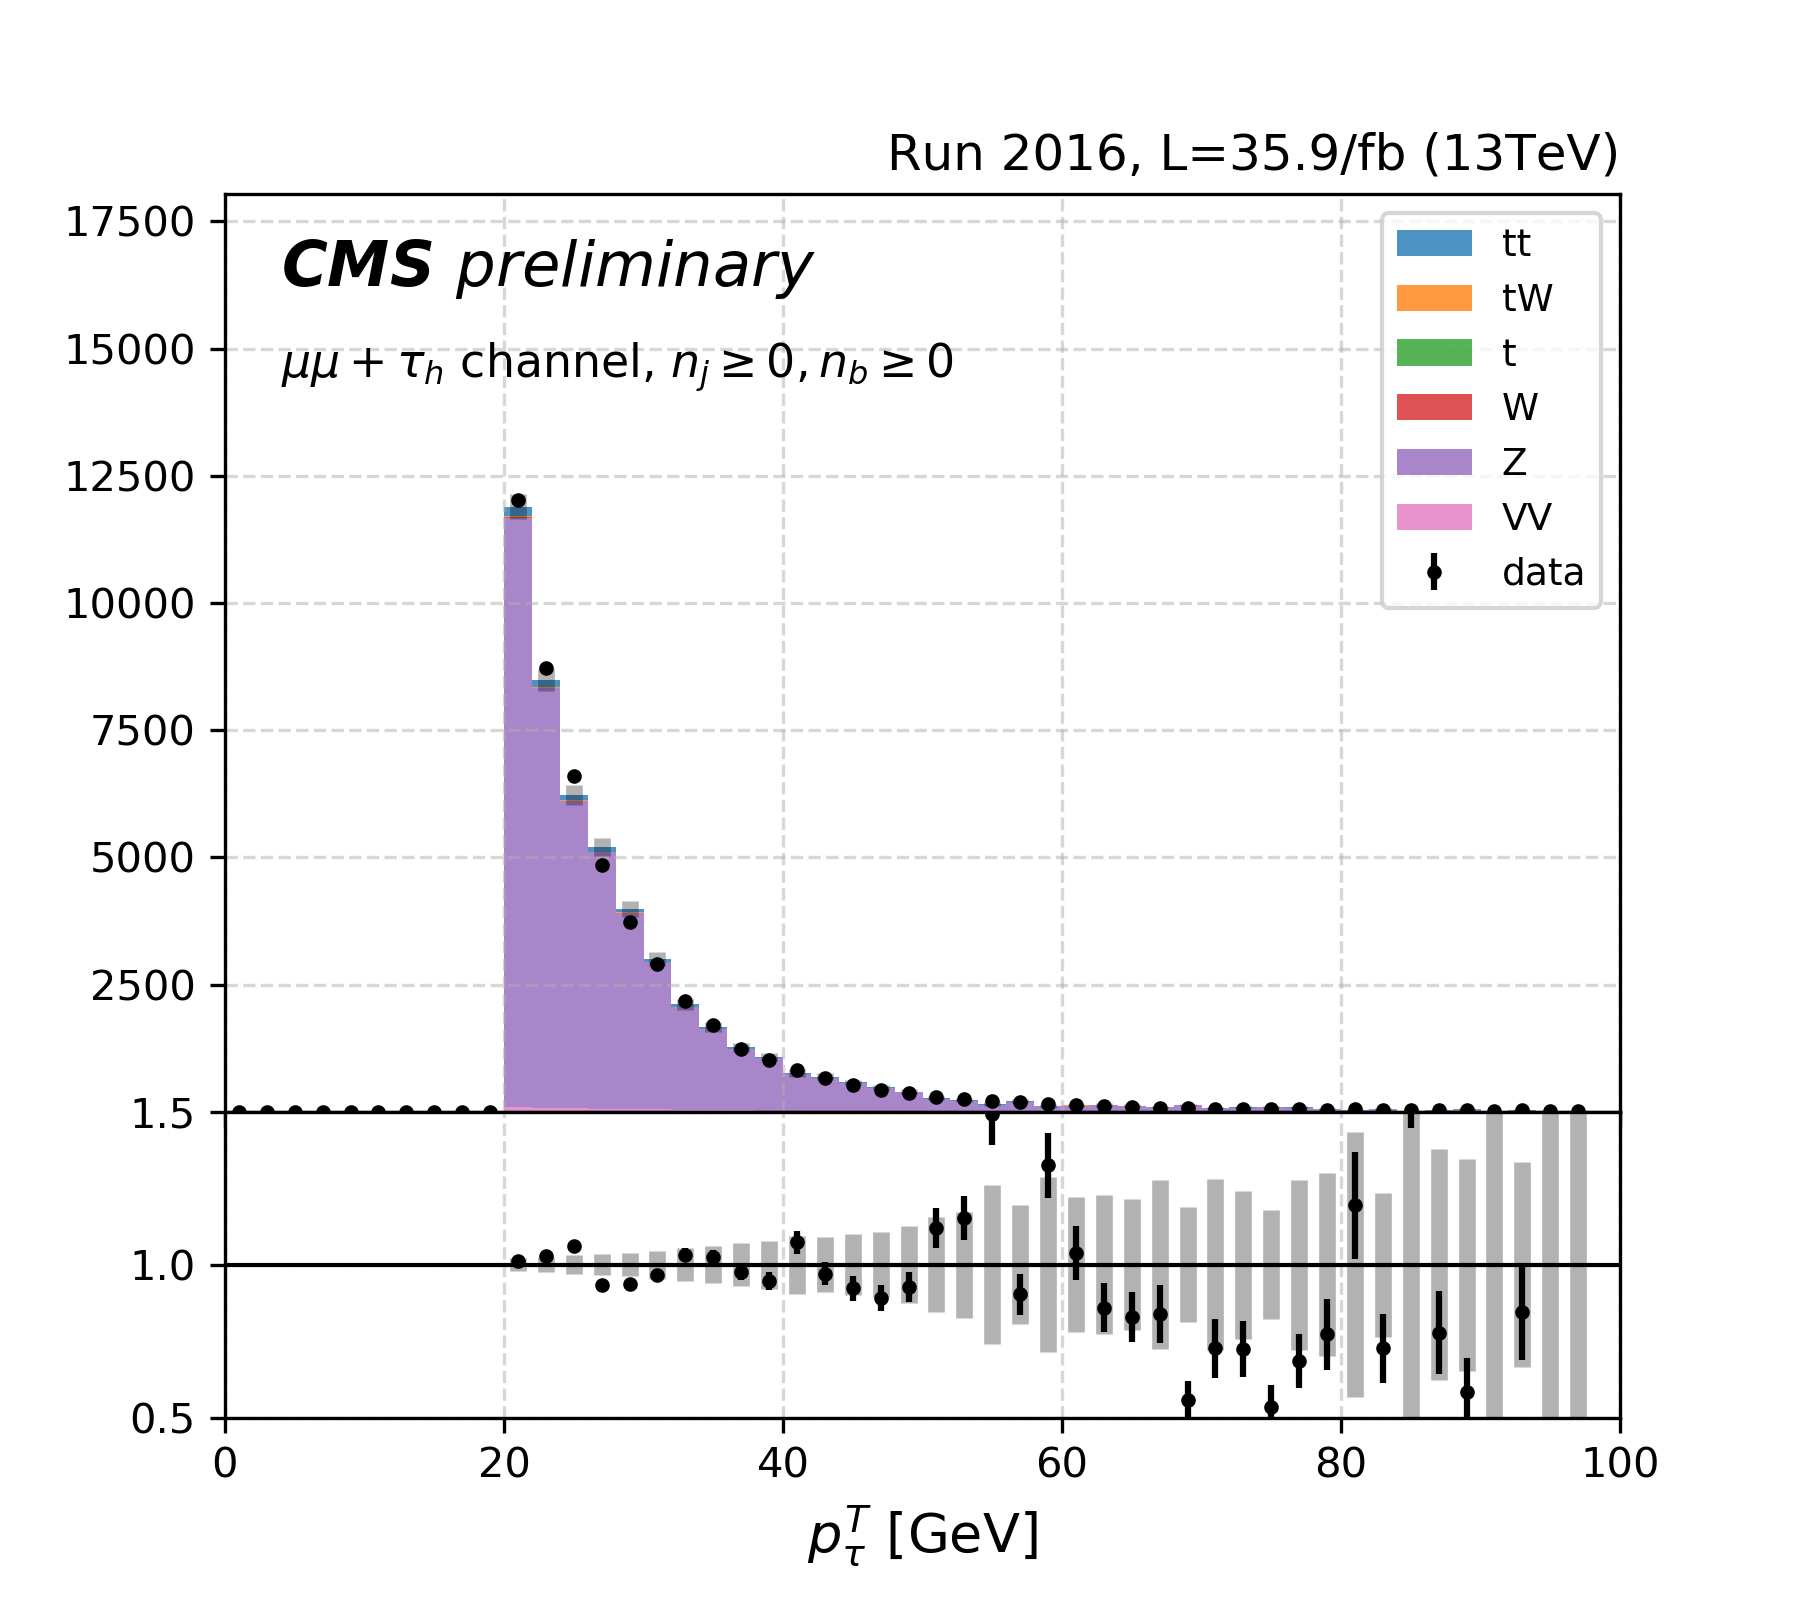
\includegraphics[width=0.4\textwidth]{chapters/Analysis/sectionCalibration/figures/jetToTauh/mumutau_tauPt_pickles_lltauVTight.png}
    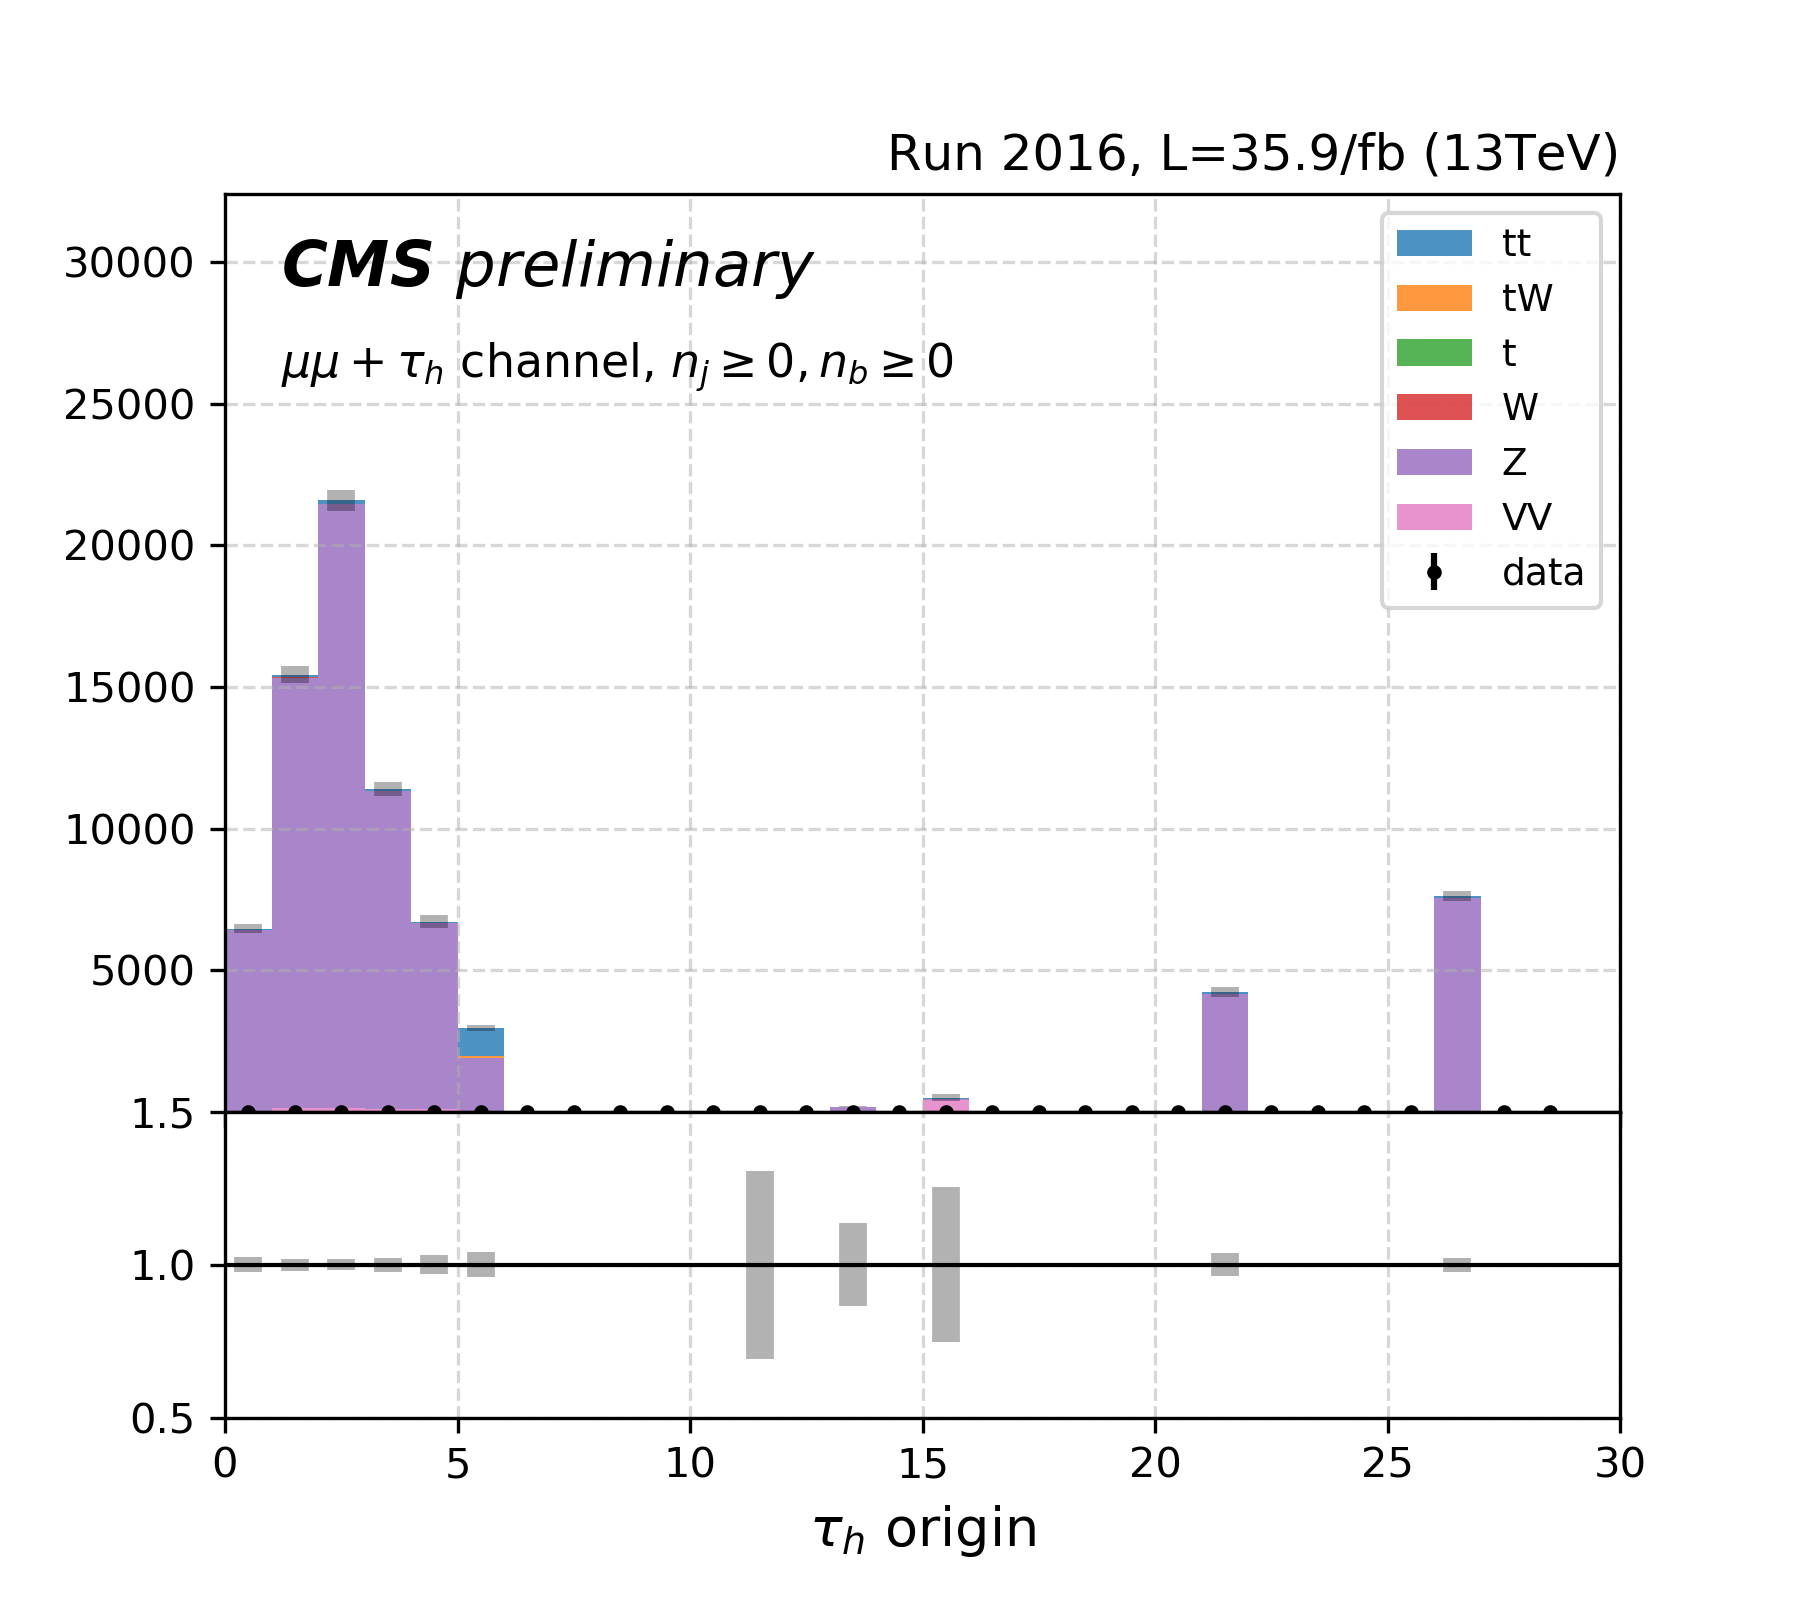
\includegraphics[width=0.4\textwidth]{chapters/Analysis/sectionCalibration/figures/jetToTauh/mumutau_tauGenFlavor_pickles_lltauTight.png}
    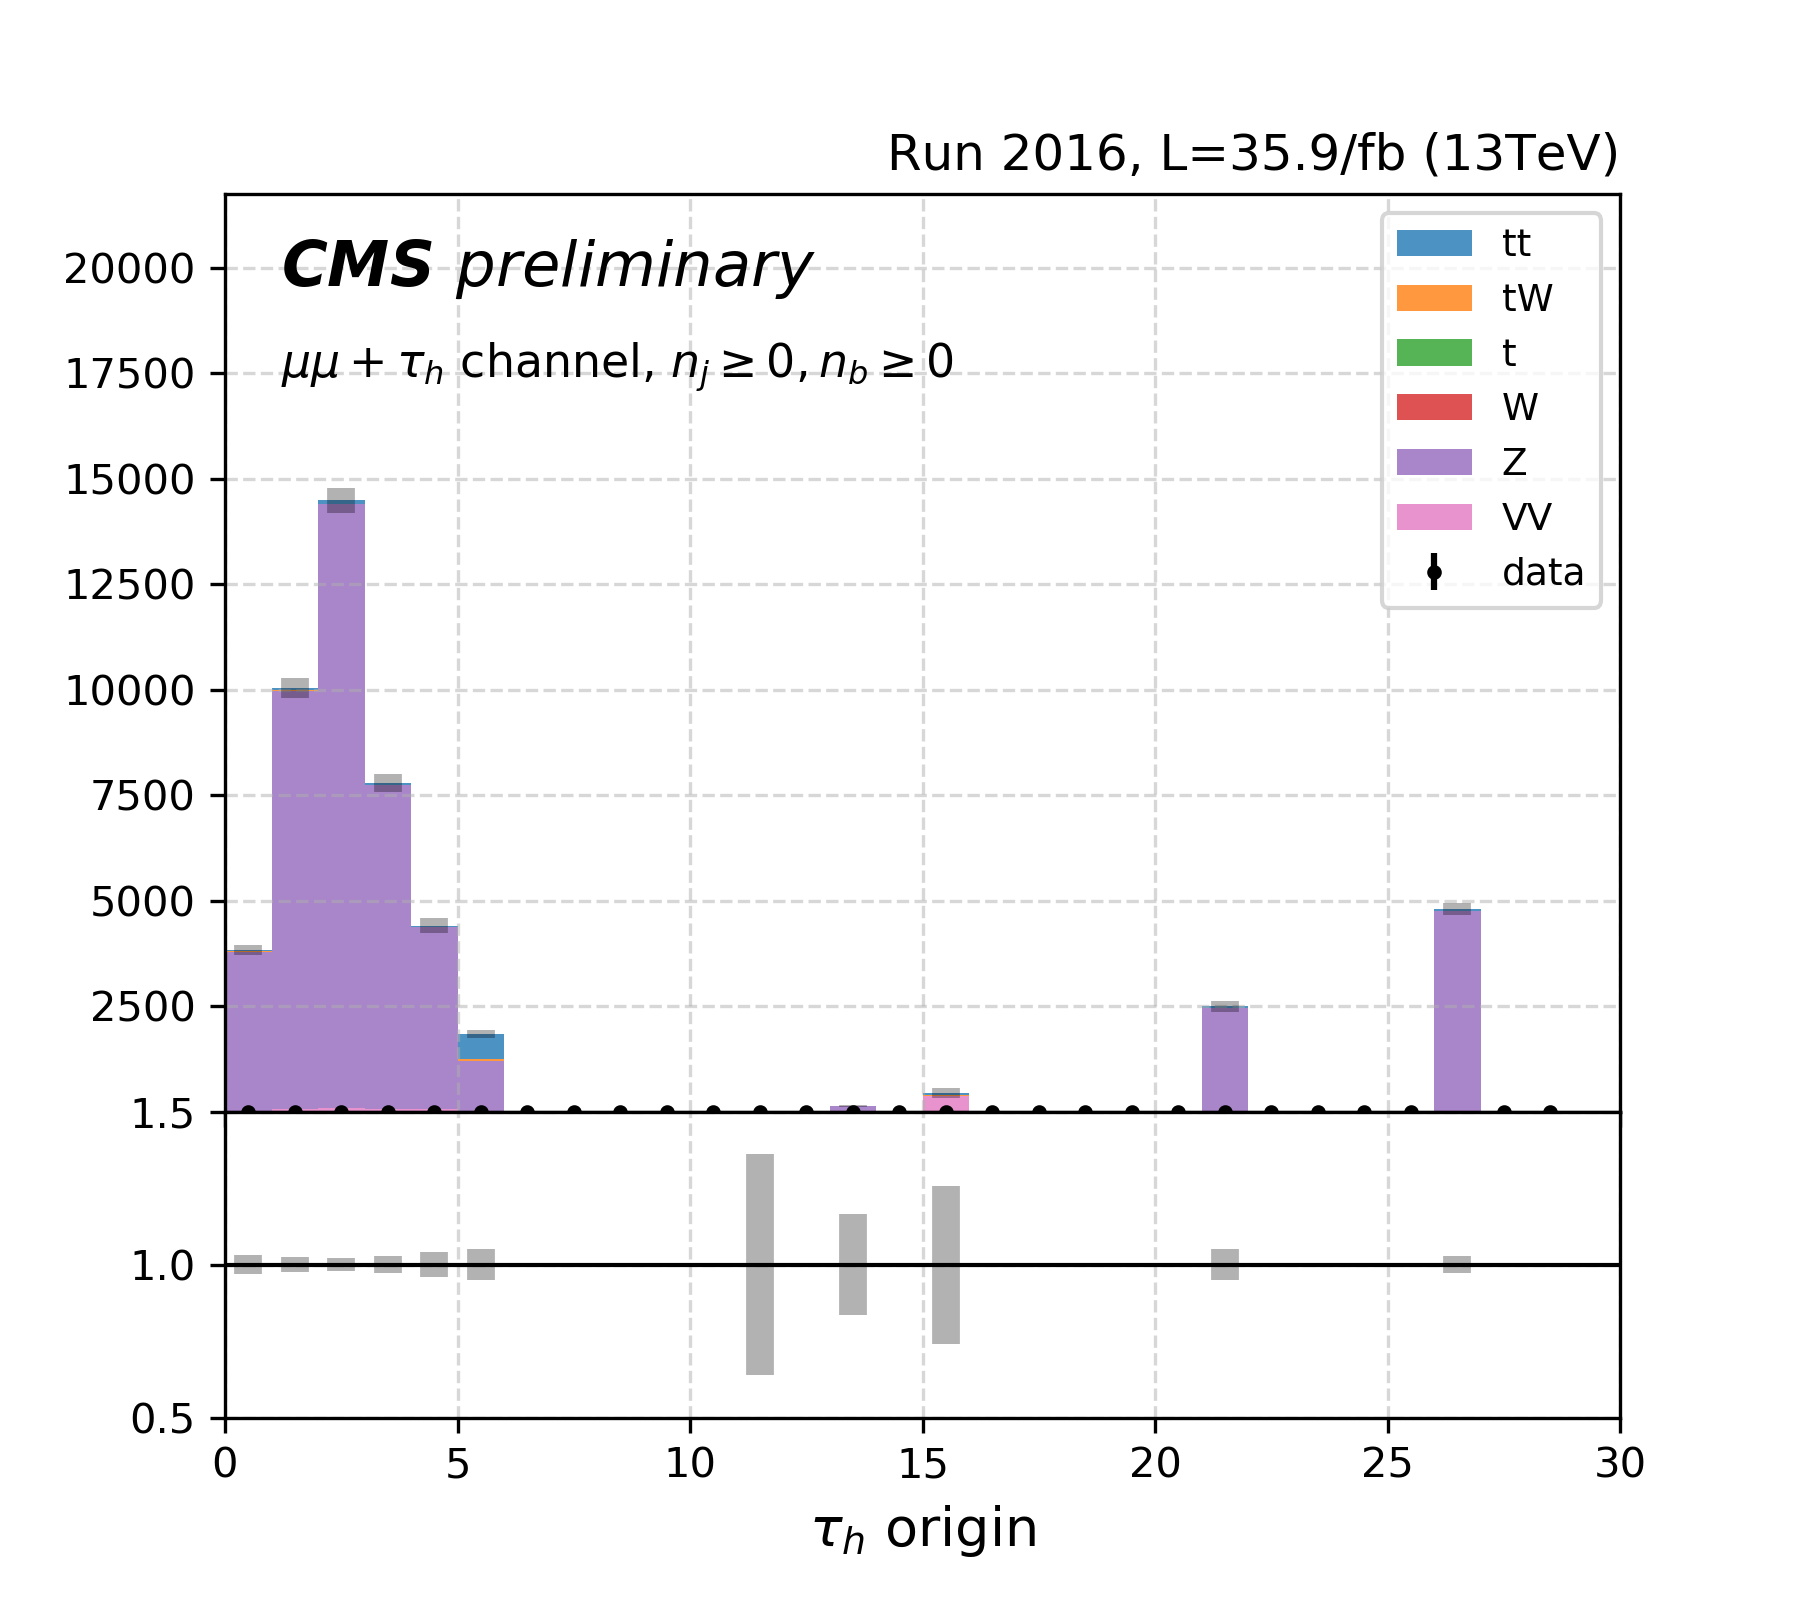
\includegraphics[width=0.4\textwidth]{chapters/Analysis/sectionCalibration/figures/jetToTauh/mumutau_tauGenFlavor_pickles_lltauVTight.png}
    \caption{Distributions of $m_{\mu\mu}$, $\tau_h$ \pt and gen-level $\tau_h$ origin in the $\mu\mu+\tau$ channel. The left and right column shows the Tight and VTight $\tau_h$ WP respectively.}
    \label{fig:appendix:fakeTauId:mumutau}
\end{figure}


\begin{figure}
    \centering
    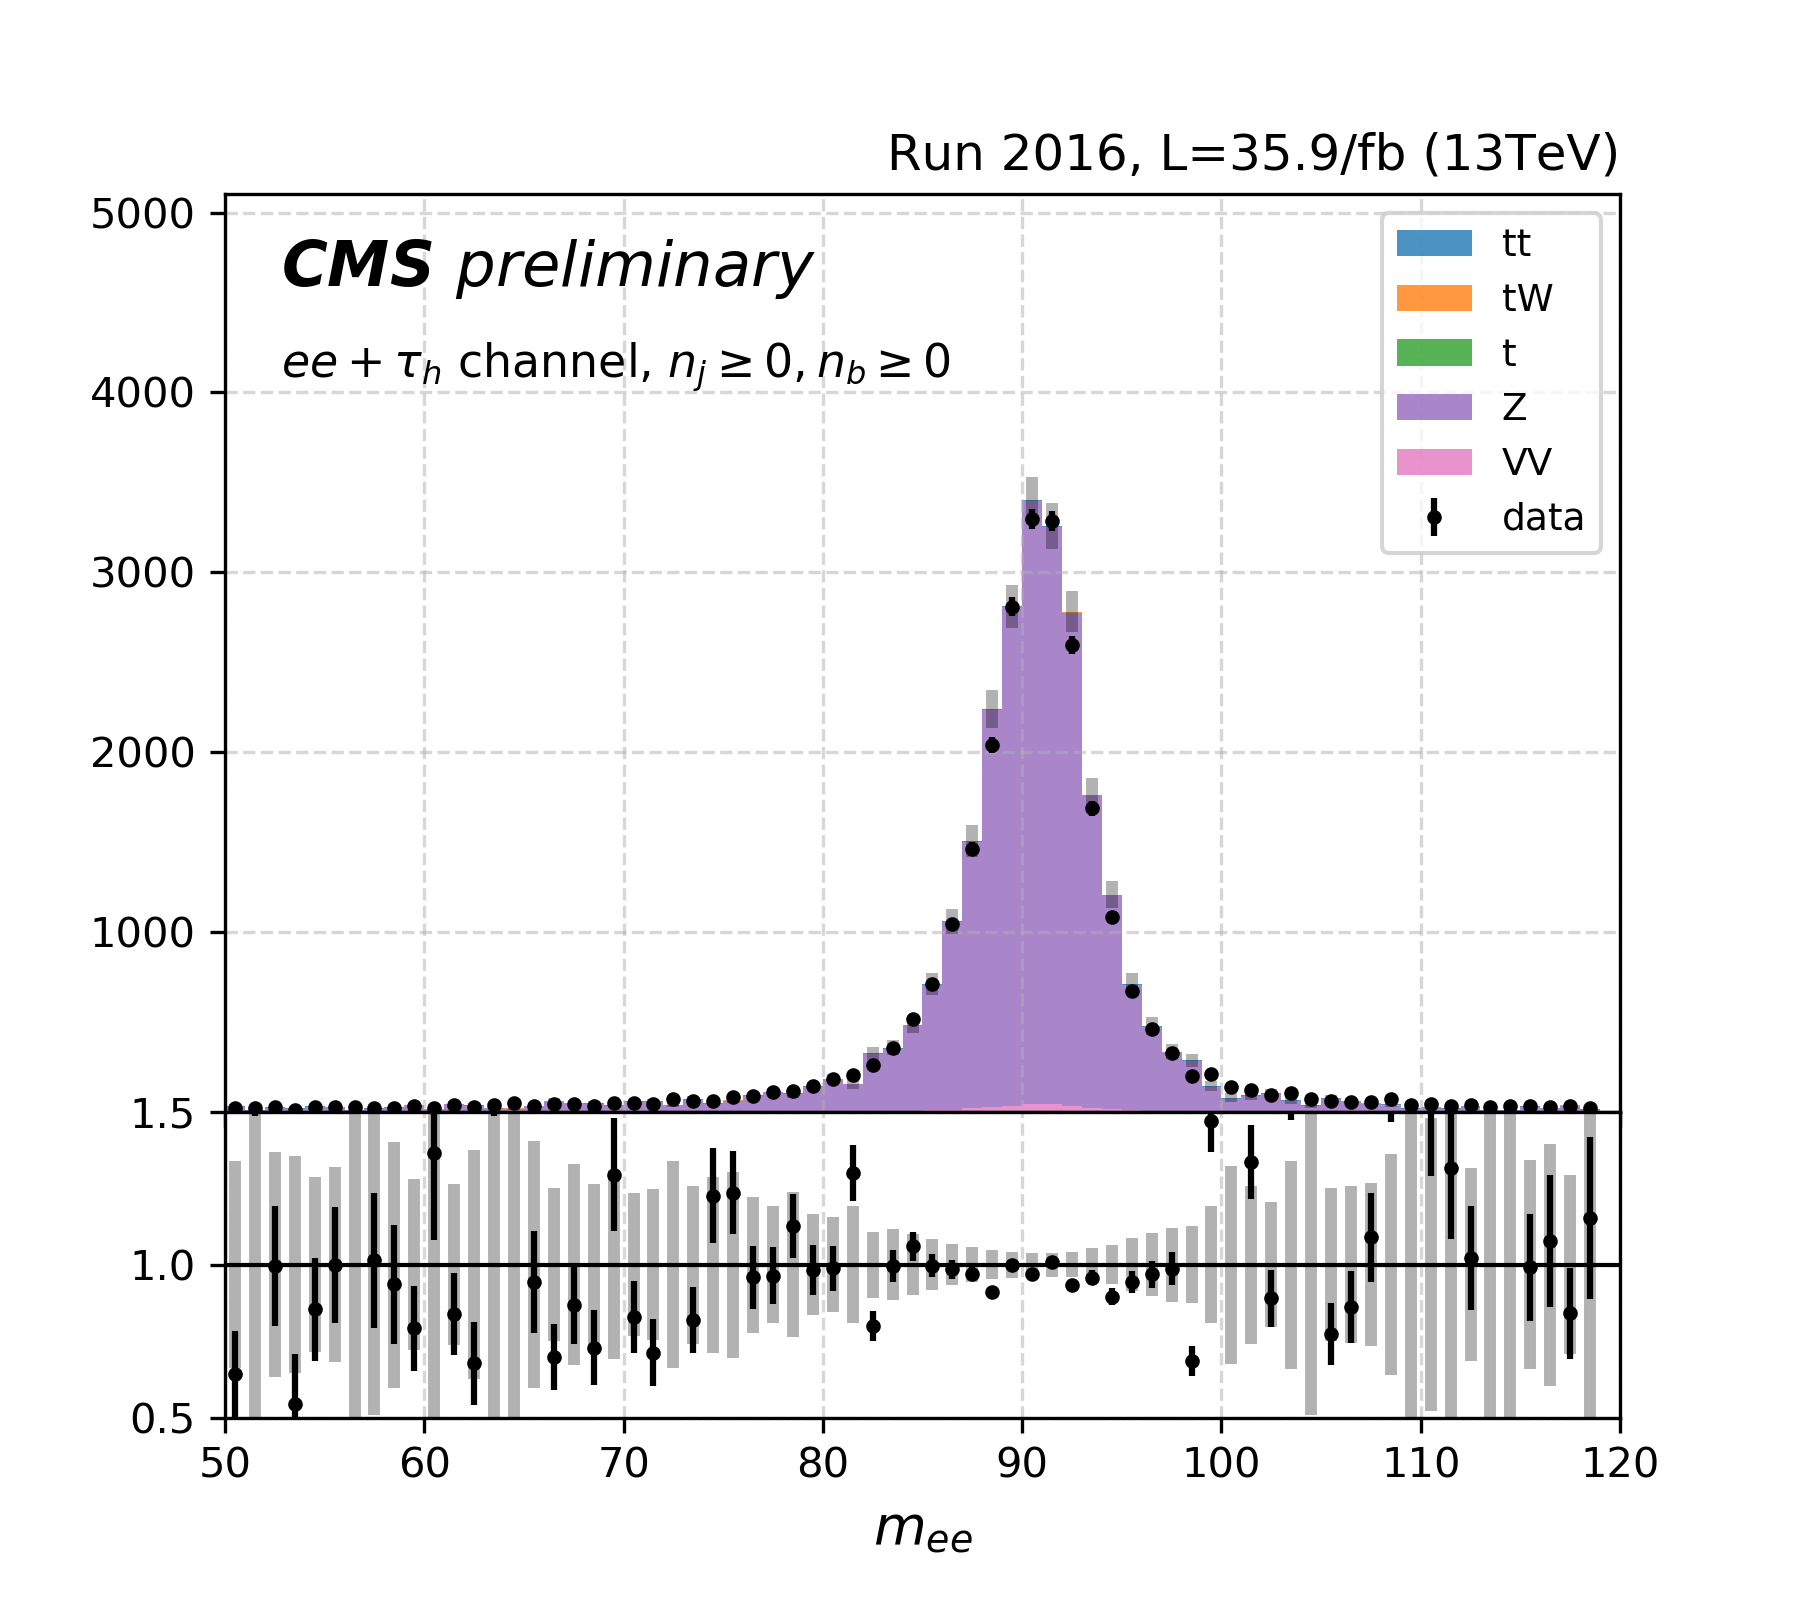
\includegraphics[width=0.4\textwidth]{chapters/Analysis/sectionCalibration/figures/jetToTauh/eetau_dilepton_mass_pickles_lltauTight.png}
    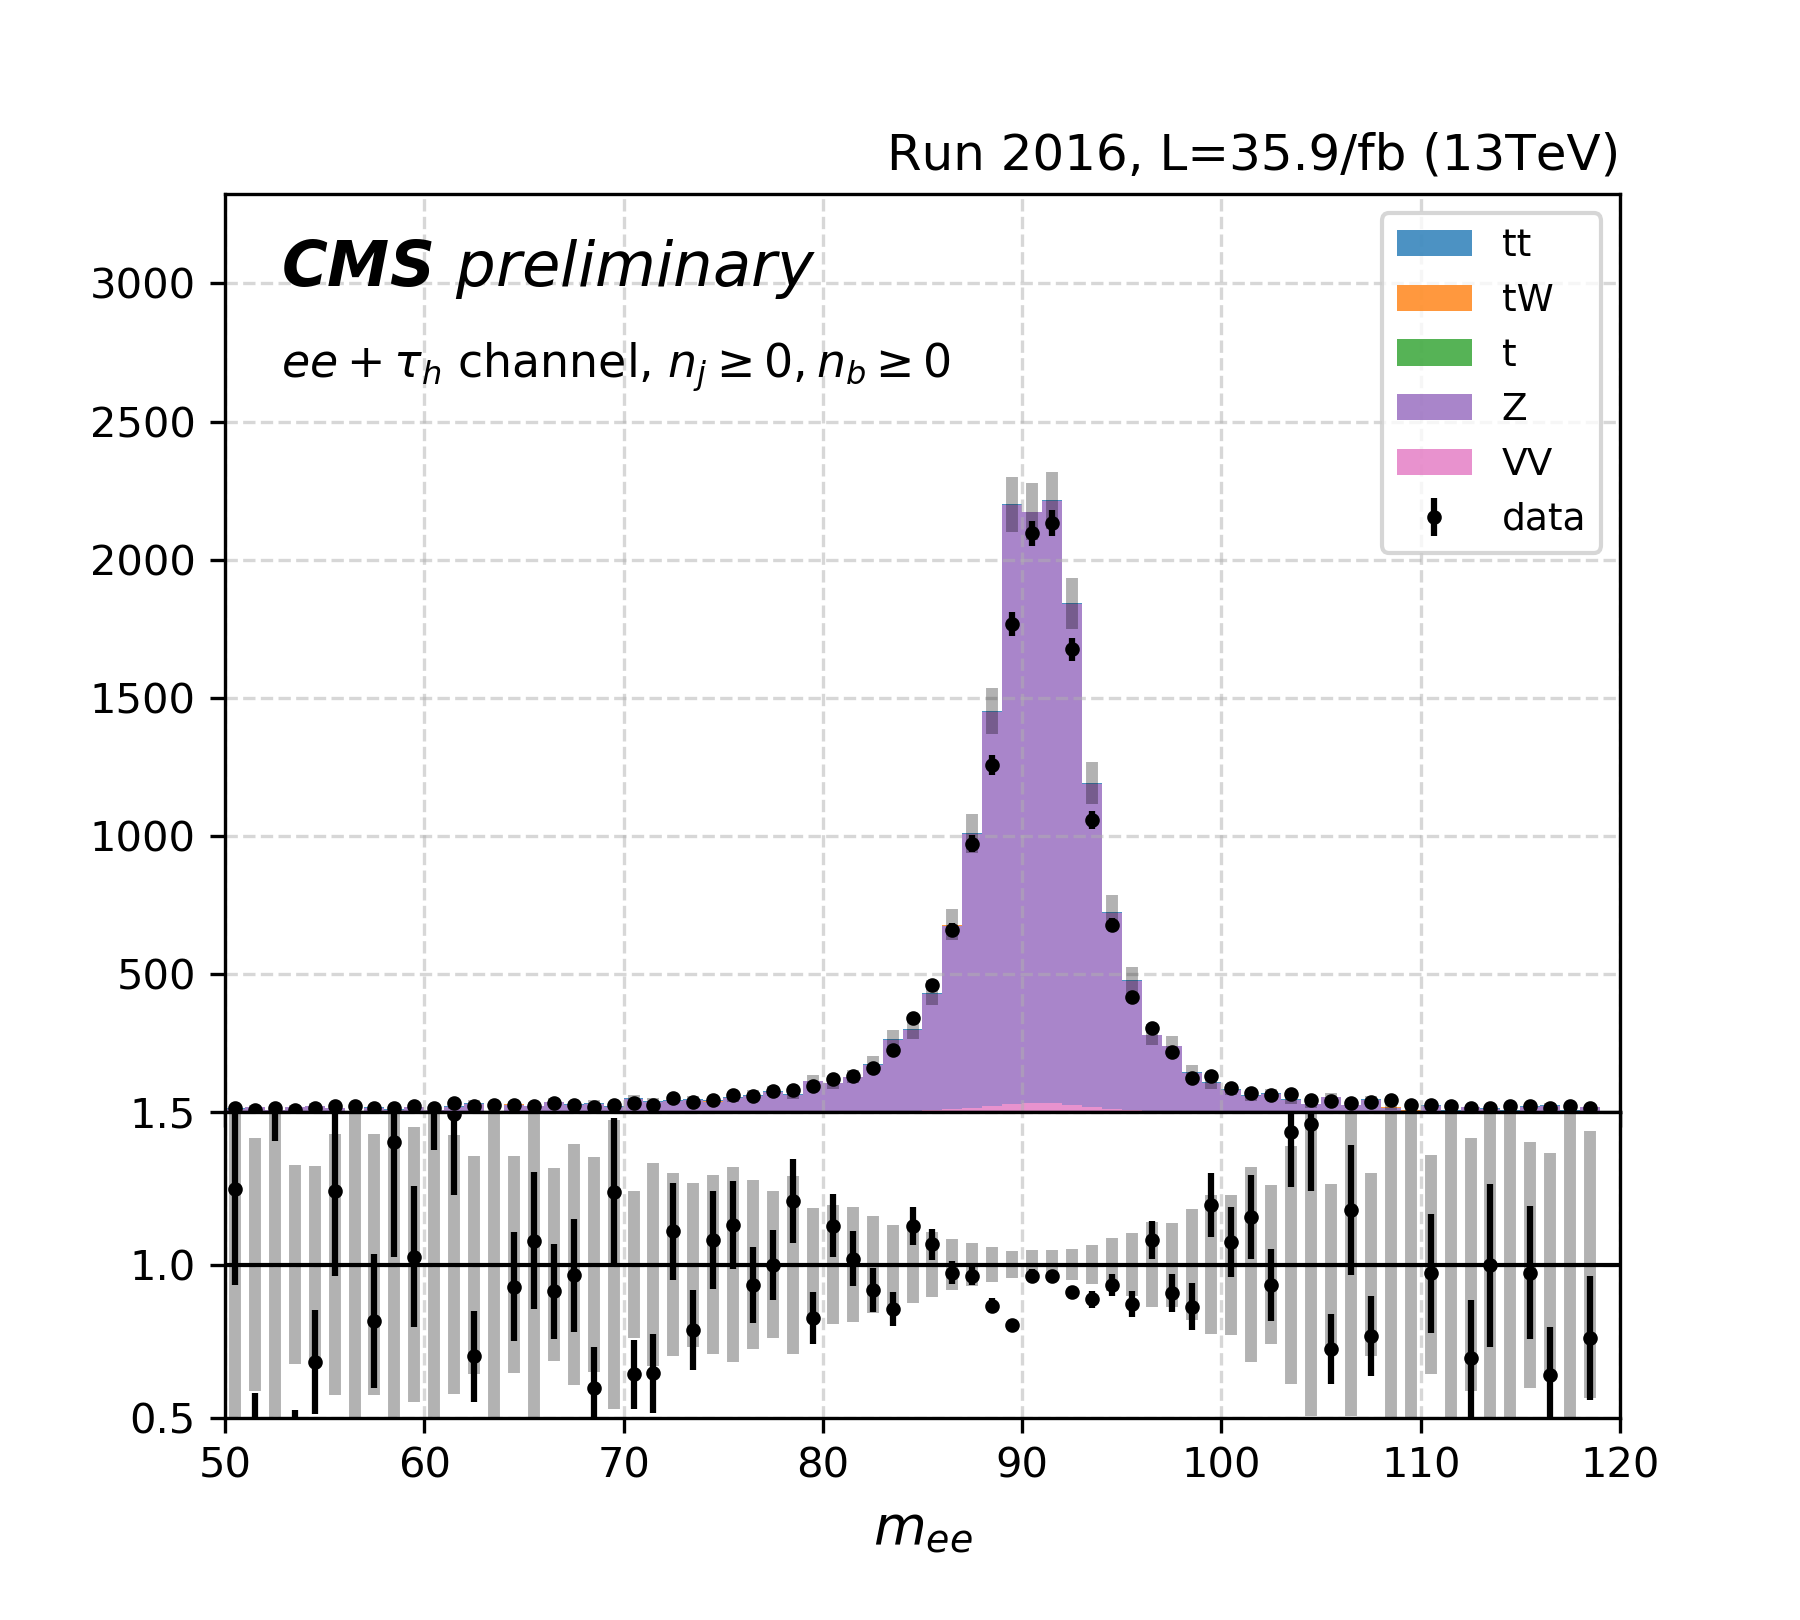
\includegraphics[width=0.4\textwidth]{chapters/Analysis/sectionCalibration/figures/jetToTauh/eetau_dilepton_mass_pickles_lltauVTight.png}
    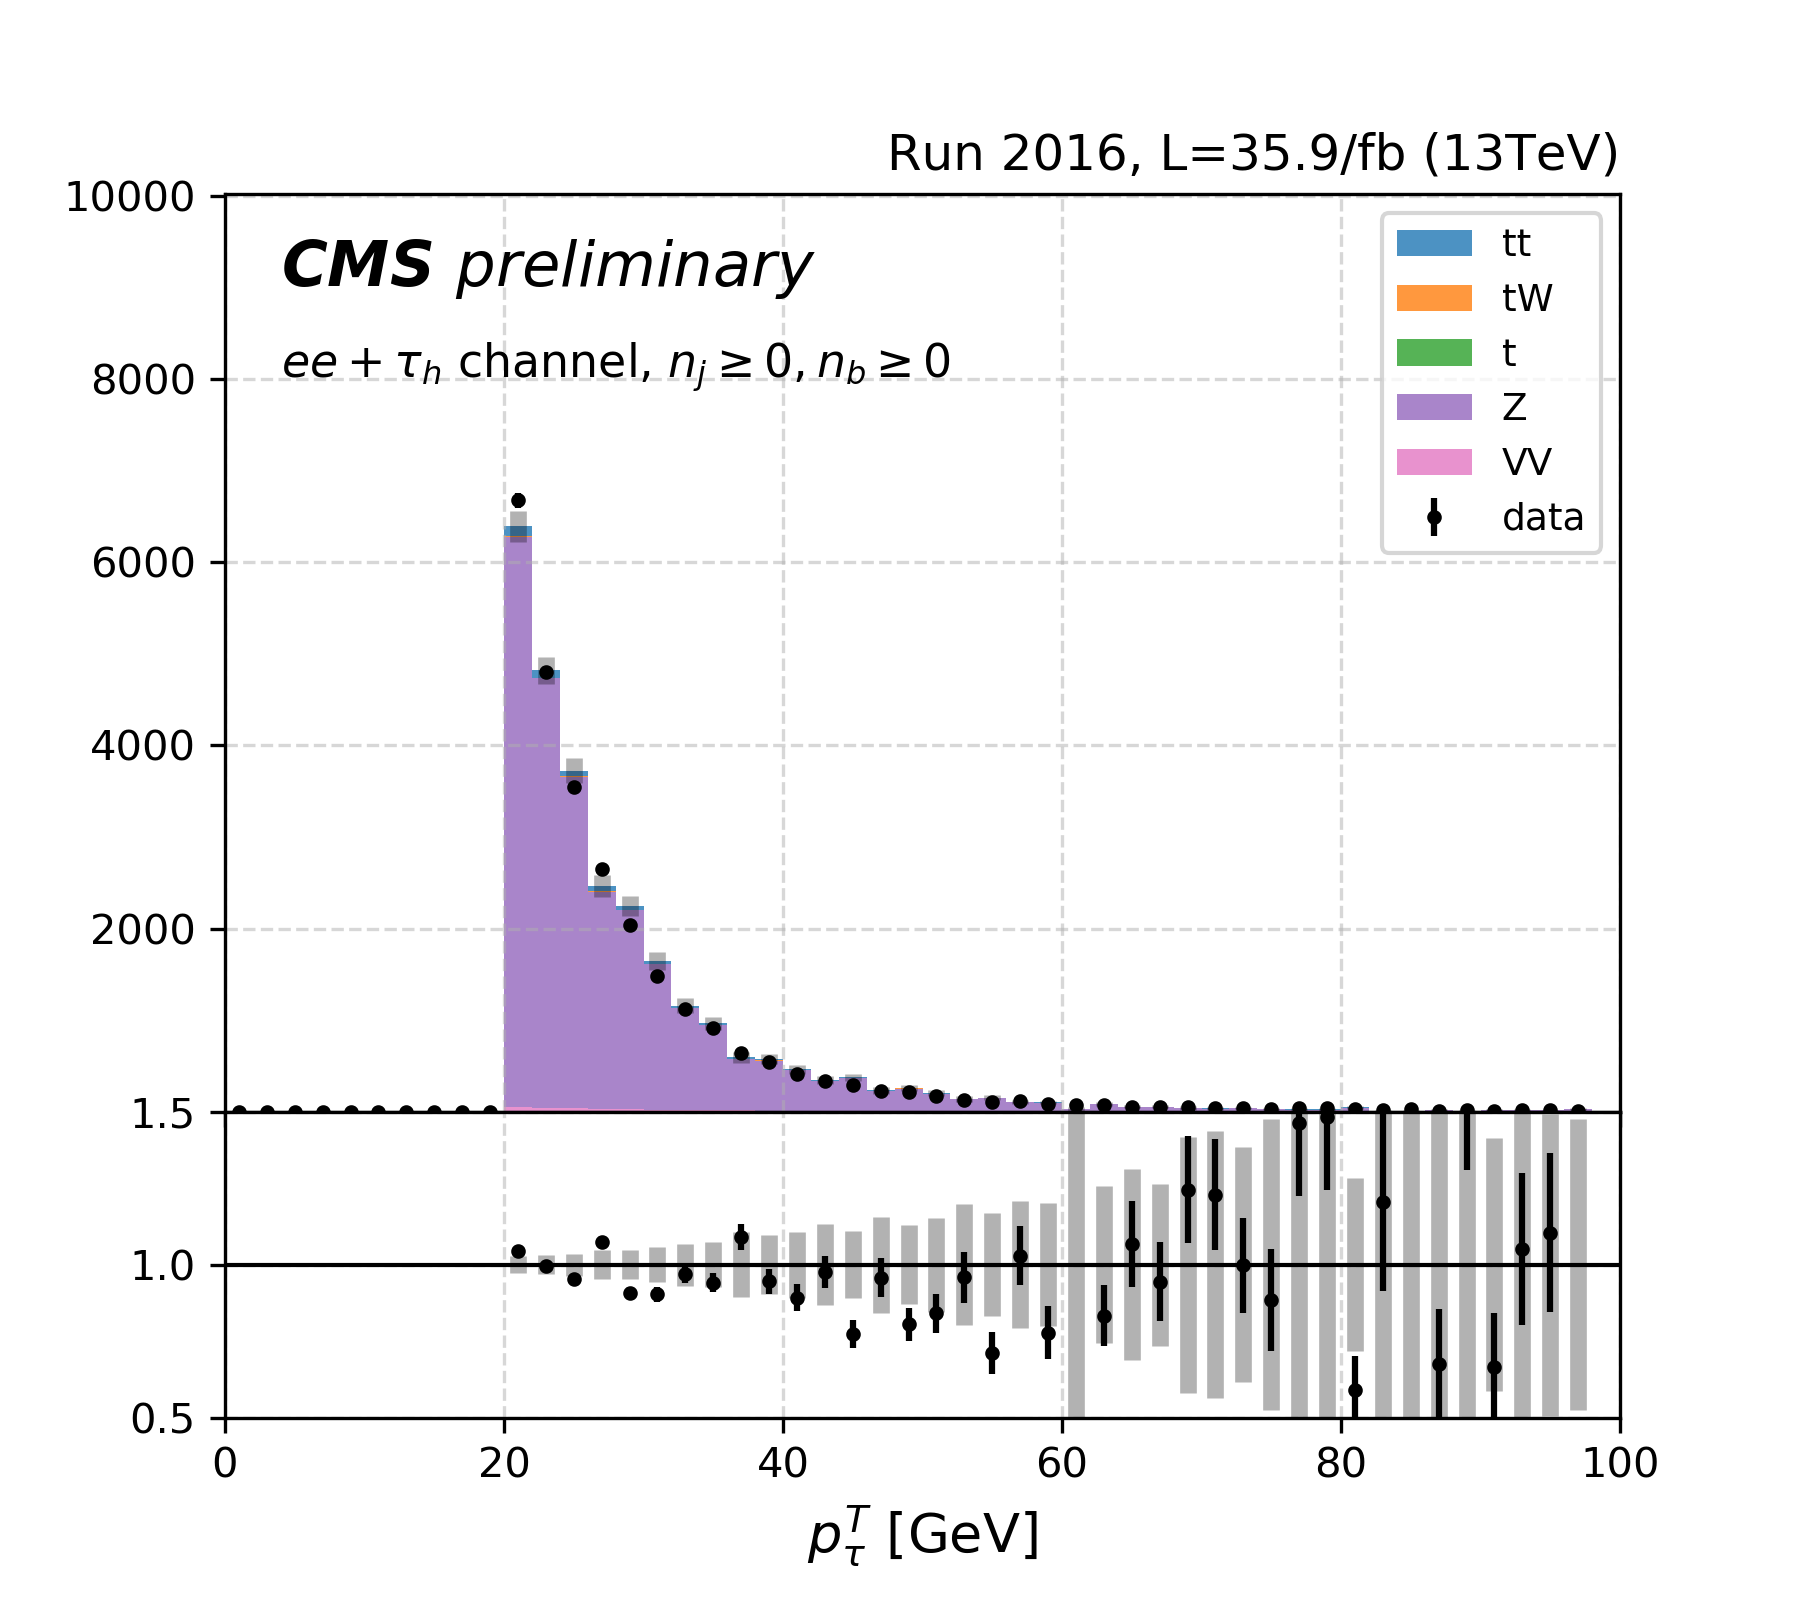
\includegraphics[width=0.4\textwidth]{chapters/Analysis/sectionCalibration/figures/jetToTauh/eetau_tauPt_pickles_lltauTight.png}
    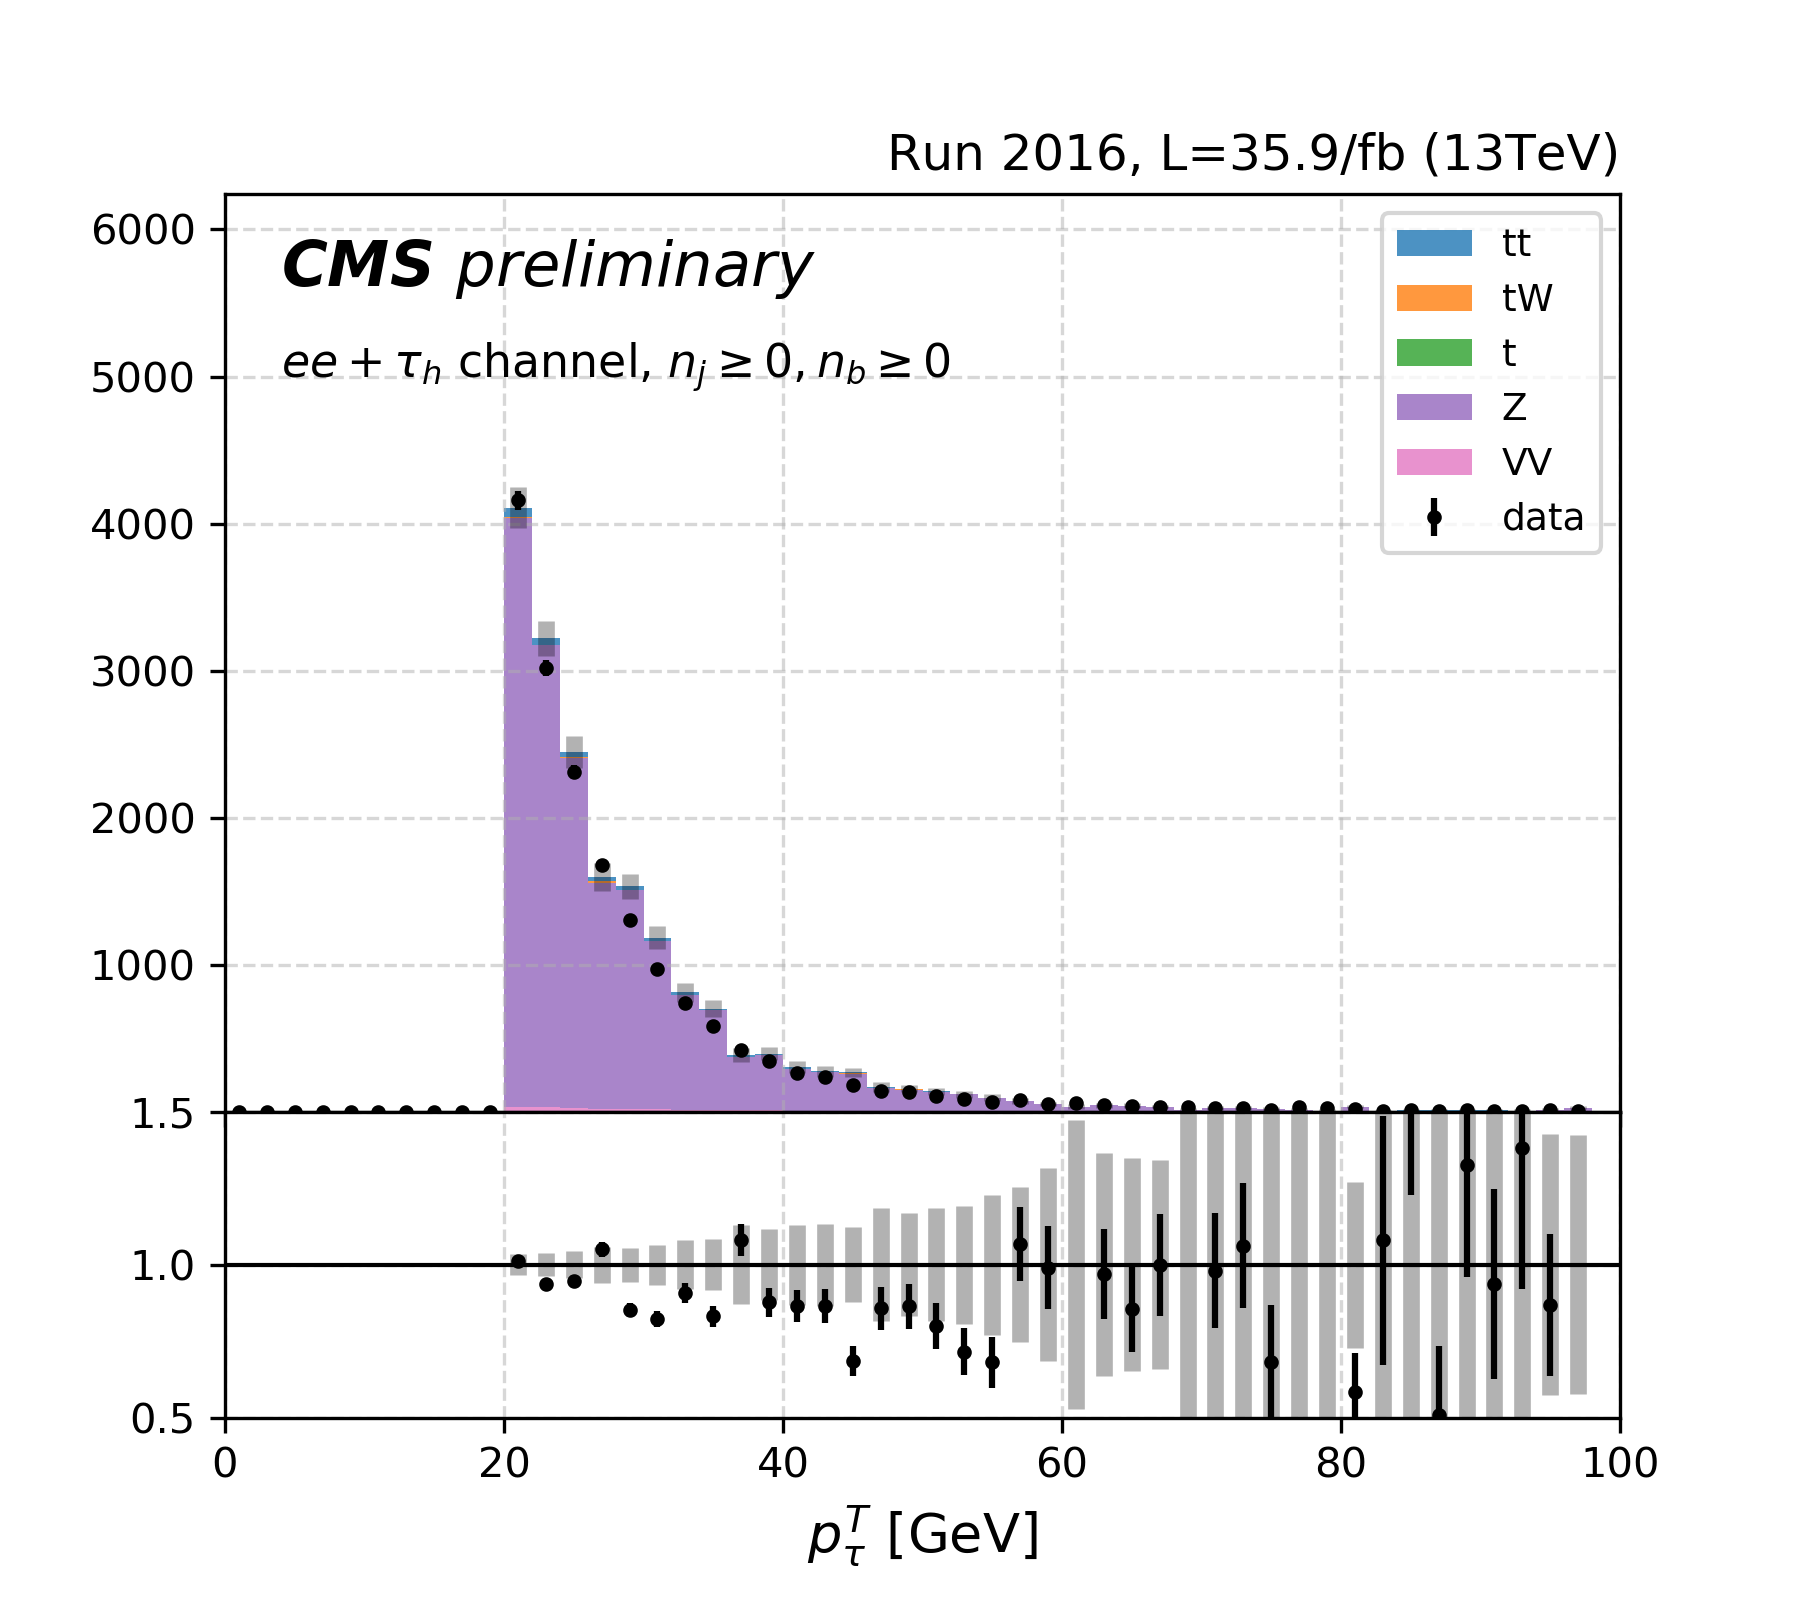
\includegraphics[width=0.4\textwidth]{chapters/Analysis/sectionCalibration/figures/jetToTauh/eetau_tauPt_pickles_lltauVTight.png}
    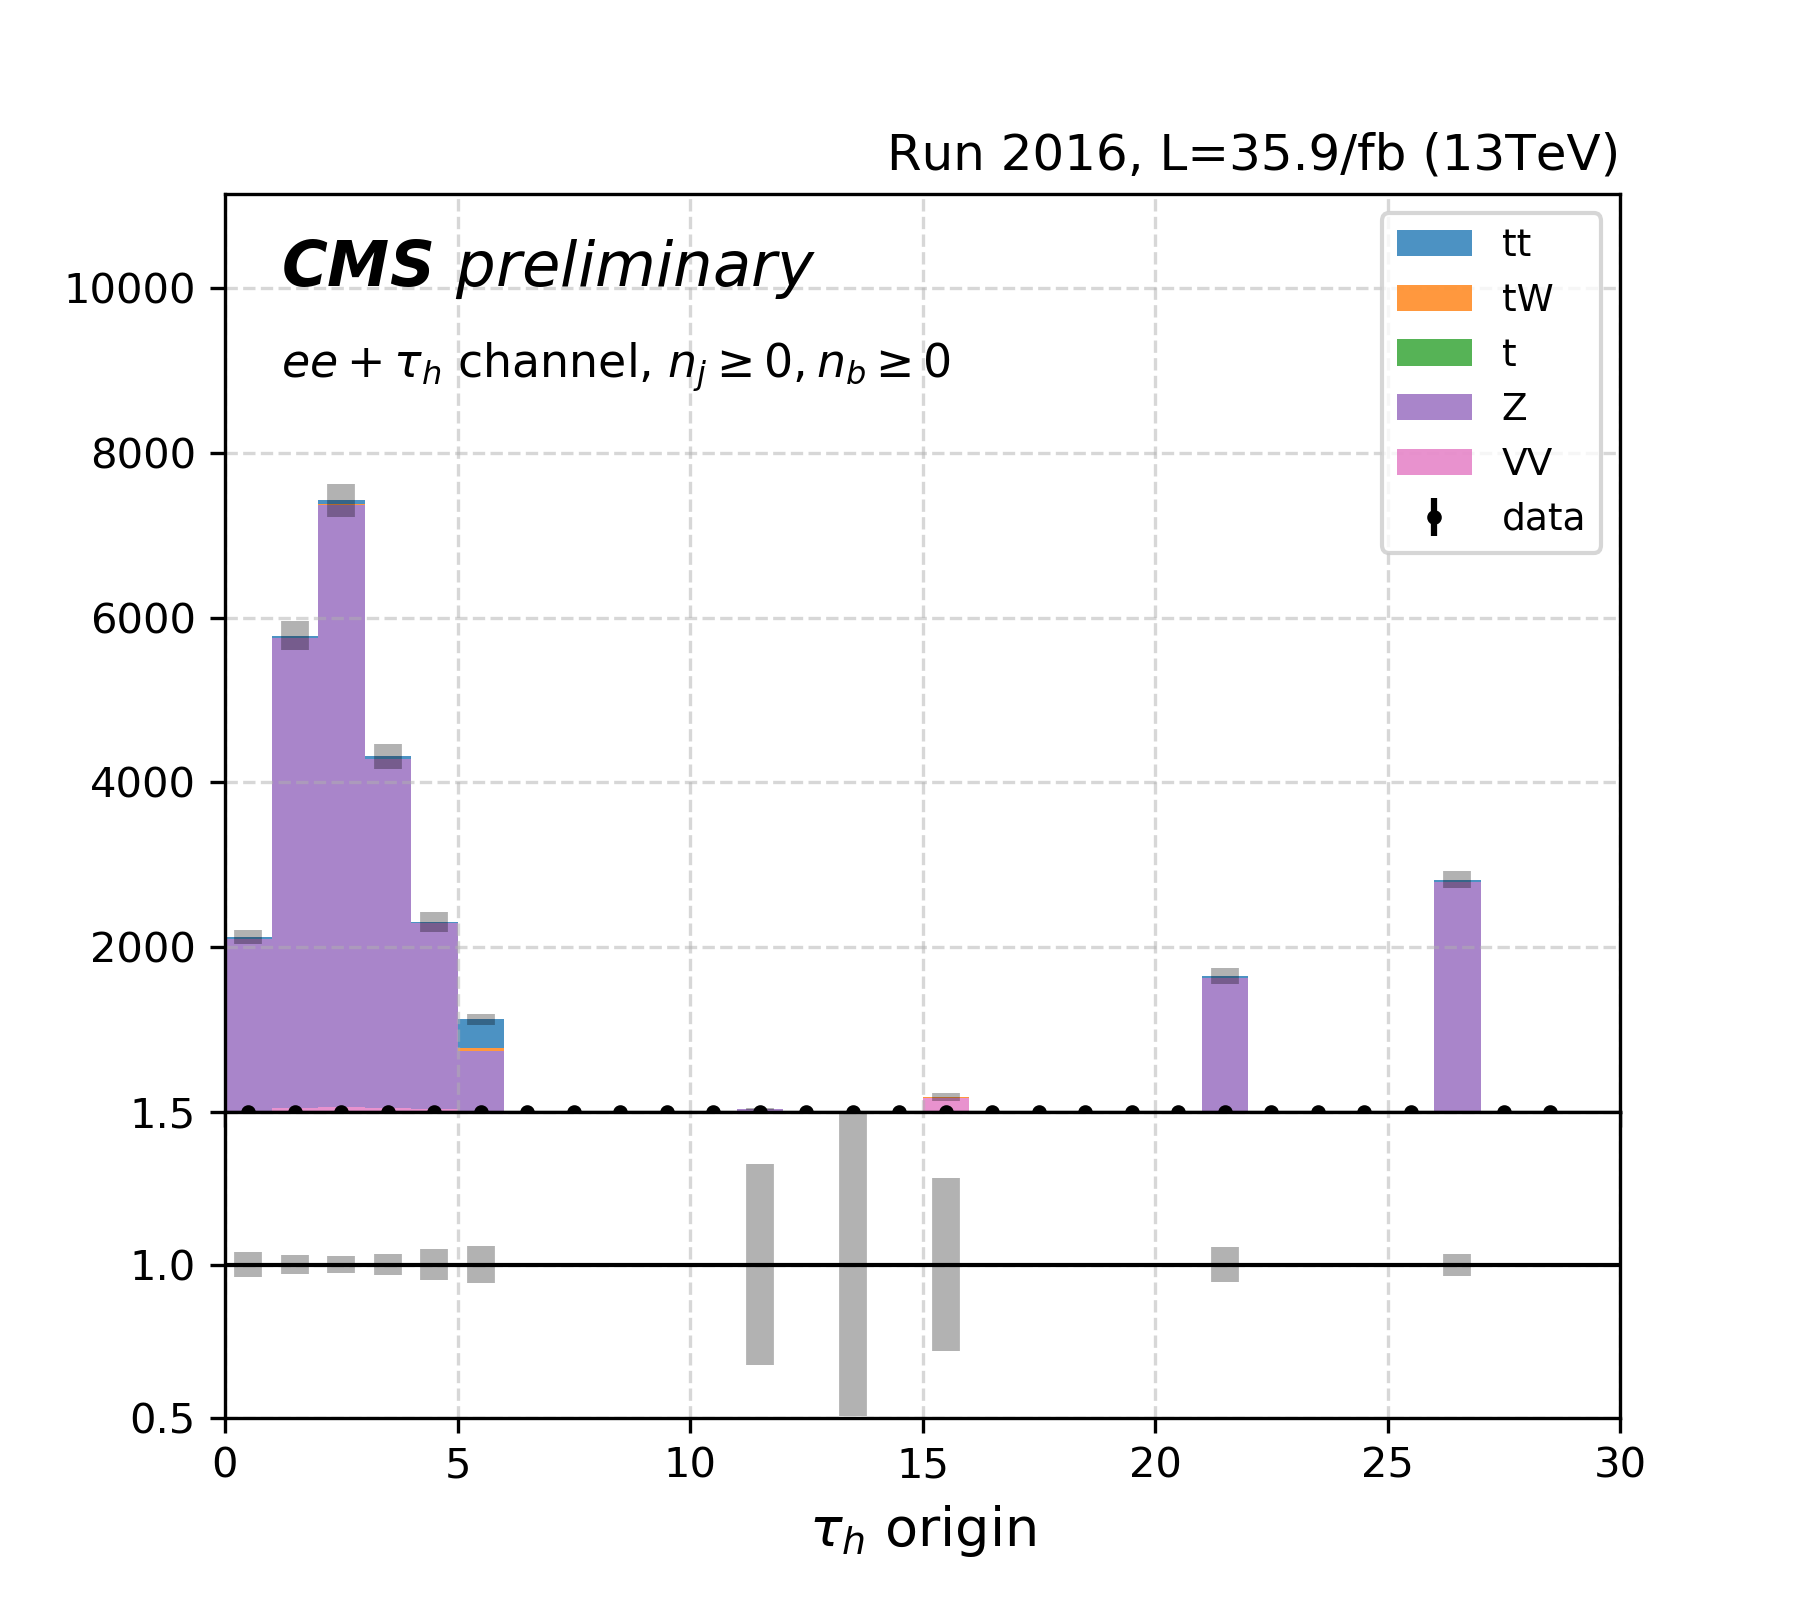
\includegraphics[width=0.4\textwidth]{chapters/Analysis/sectionCalibration/figures/jetToTauh/eetau_tauGenFlavor_pickles_lltauTight.png}
    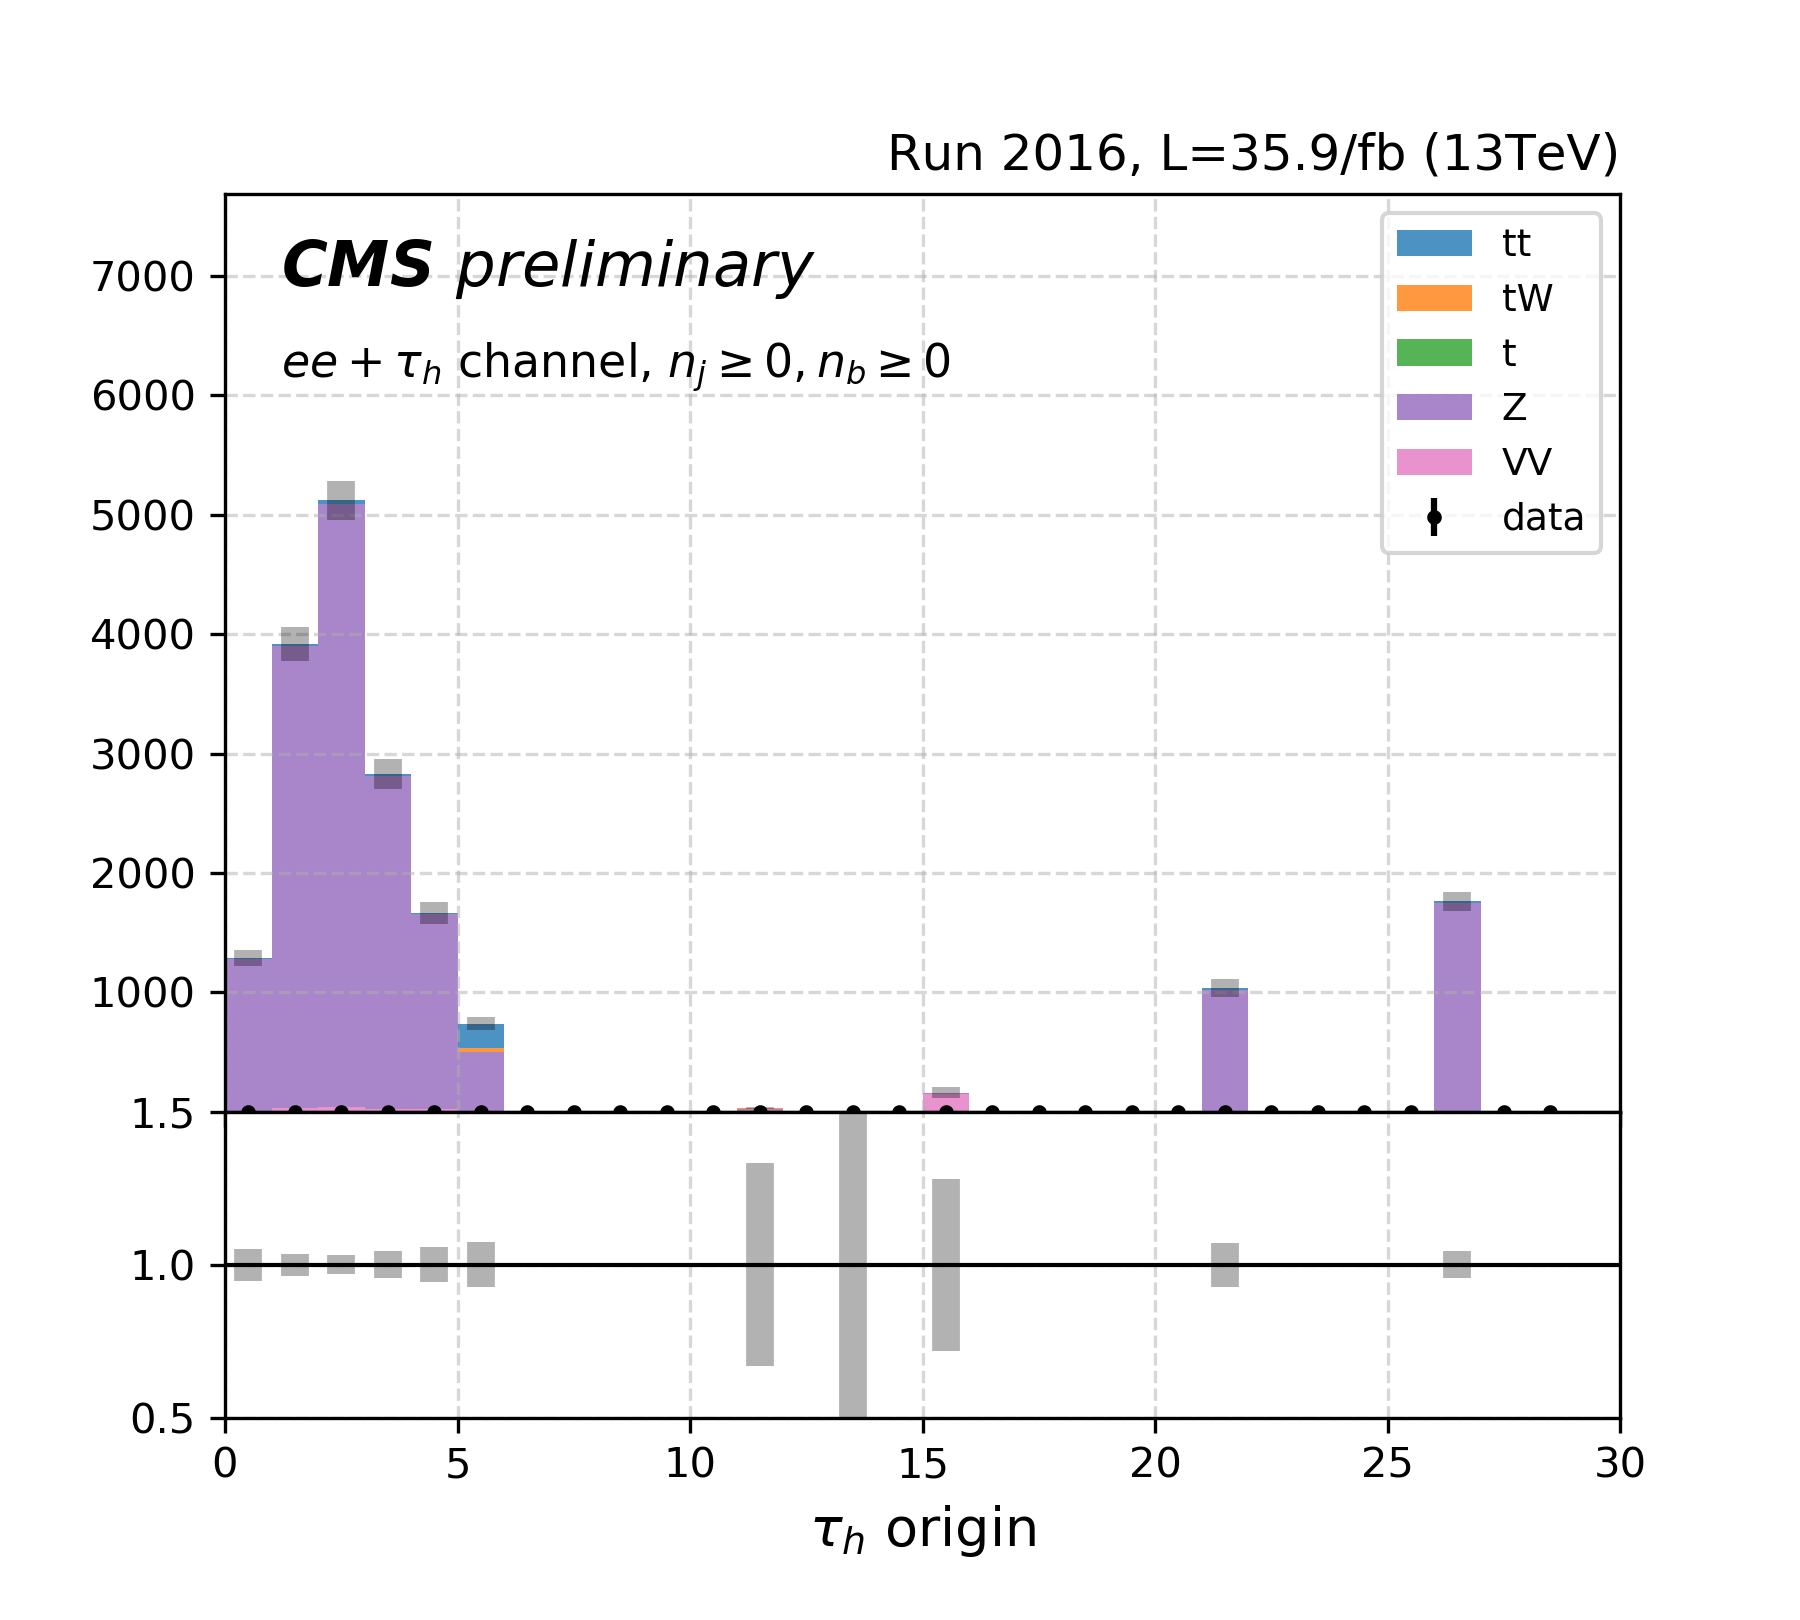
\includegraphics[width=0.4\textwidth]{chapters/Analysis/sectionCalibration/figures/jetToTauh/eetau_tauGenFlavor_pickles_lltauVTight.png}
    \caption{Distributions of $m_{ee}$, $\tau_h$ \pt and gen-level $\tau_h$ origin in the $ee+\tau$ channel. The left and right column shows the Tight and VTight $\tau_h$ WP respectively.}
    \label{fig:appendix:fakeTauId:eetau}
\end{figure}


The \pt spectrum of $\tau_h$ in $\mu\mu+\tau_h$, $ee+\tau_h$ and $e\mu+\tau_h$ final states are shown in figure~\ref{fig:misidprefit}. Because jet modeling of Z+jet is off in $n_j=0$ but good $n_j \geq 1$, the events are split into $n_j=0$ and $n_j \geq 1$ to deal with jet modeling in the Z+jet simulation. Both Tight and VTight working points for $\tau_h$ isolation are included.



\begin{figure}
    \centering
    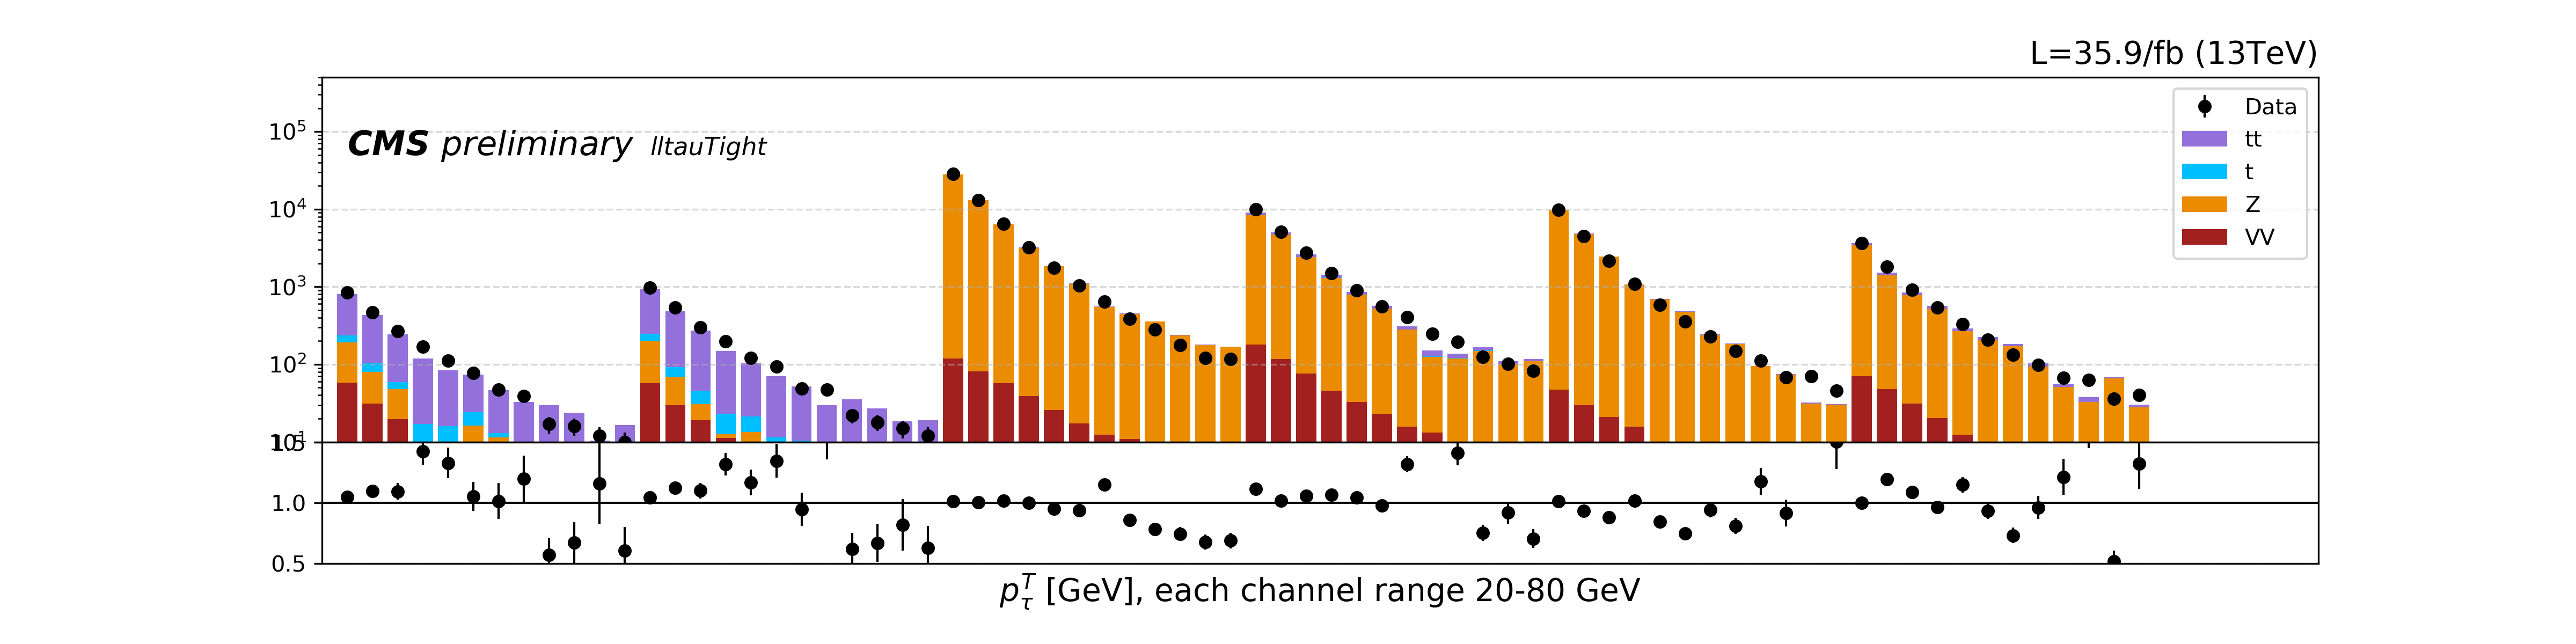
\includegraphics[width=0.99\textwidth]{chapters/Analysis/sectionCalibration/figures/jetToTauh/2020_tauID_prefit_lltauTight.png}
    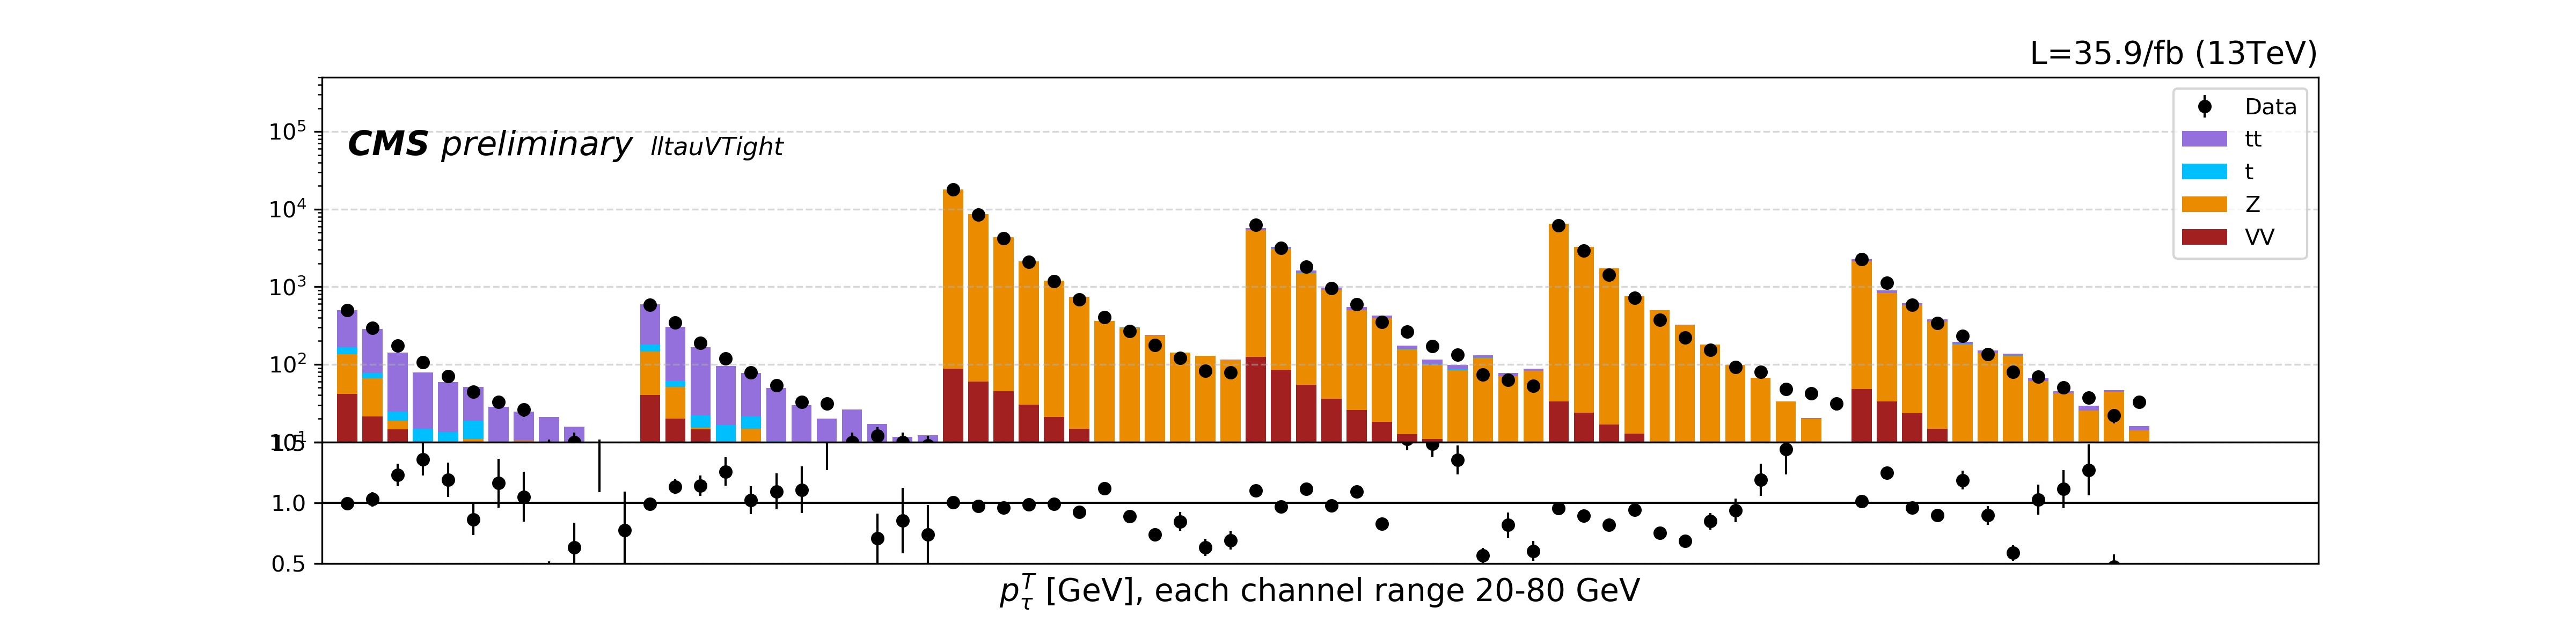
\includegraphics[width=0.99\textwidth]{chapters/Analysis/sectionCalibration/figures/jetToTauh/2020_tauID_prefit_lltauVTight.png}
    \caption{Prefit distributions of $\tau_h$ \pt. Upper and lower are the Tight and VTight WP.}
    \label{fig:appendix:fakeTauId:prefit}
\end{figure}

% \begin{figure}
%     \centering
%     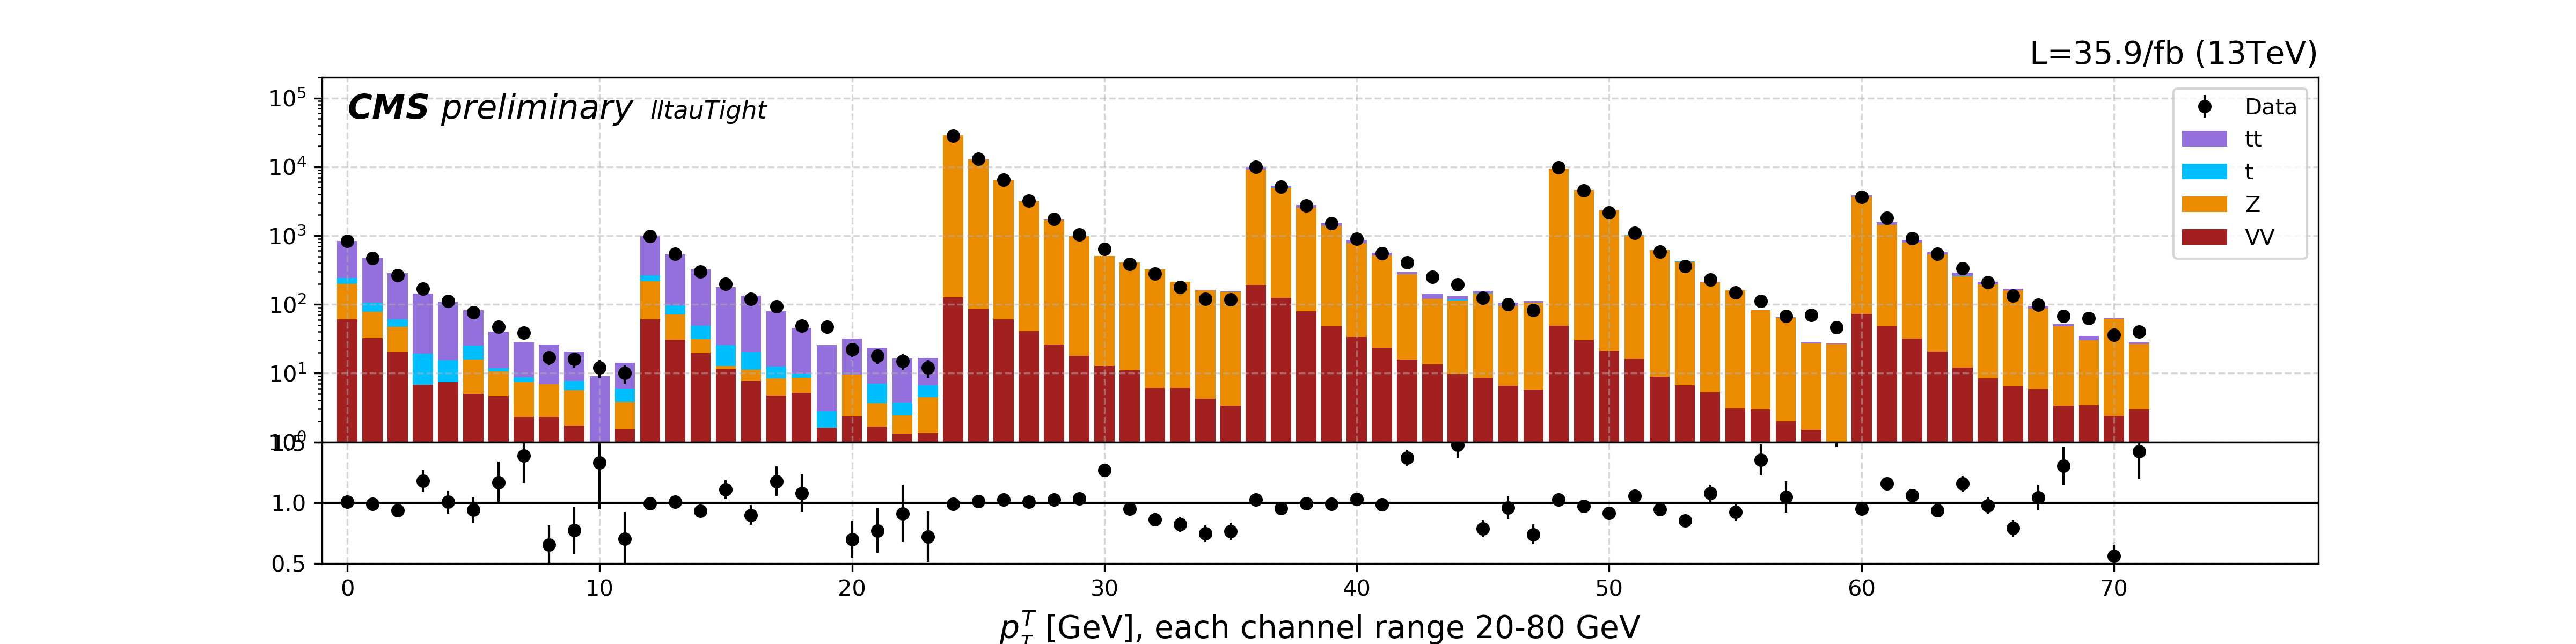
\includegraphics[width=0.99\textwidth]{chapters/Analysis/sectionCalibration/figures/jetToTauh/2020_tauID_postfit_lltauTight.png}
%     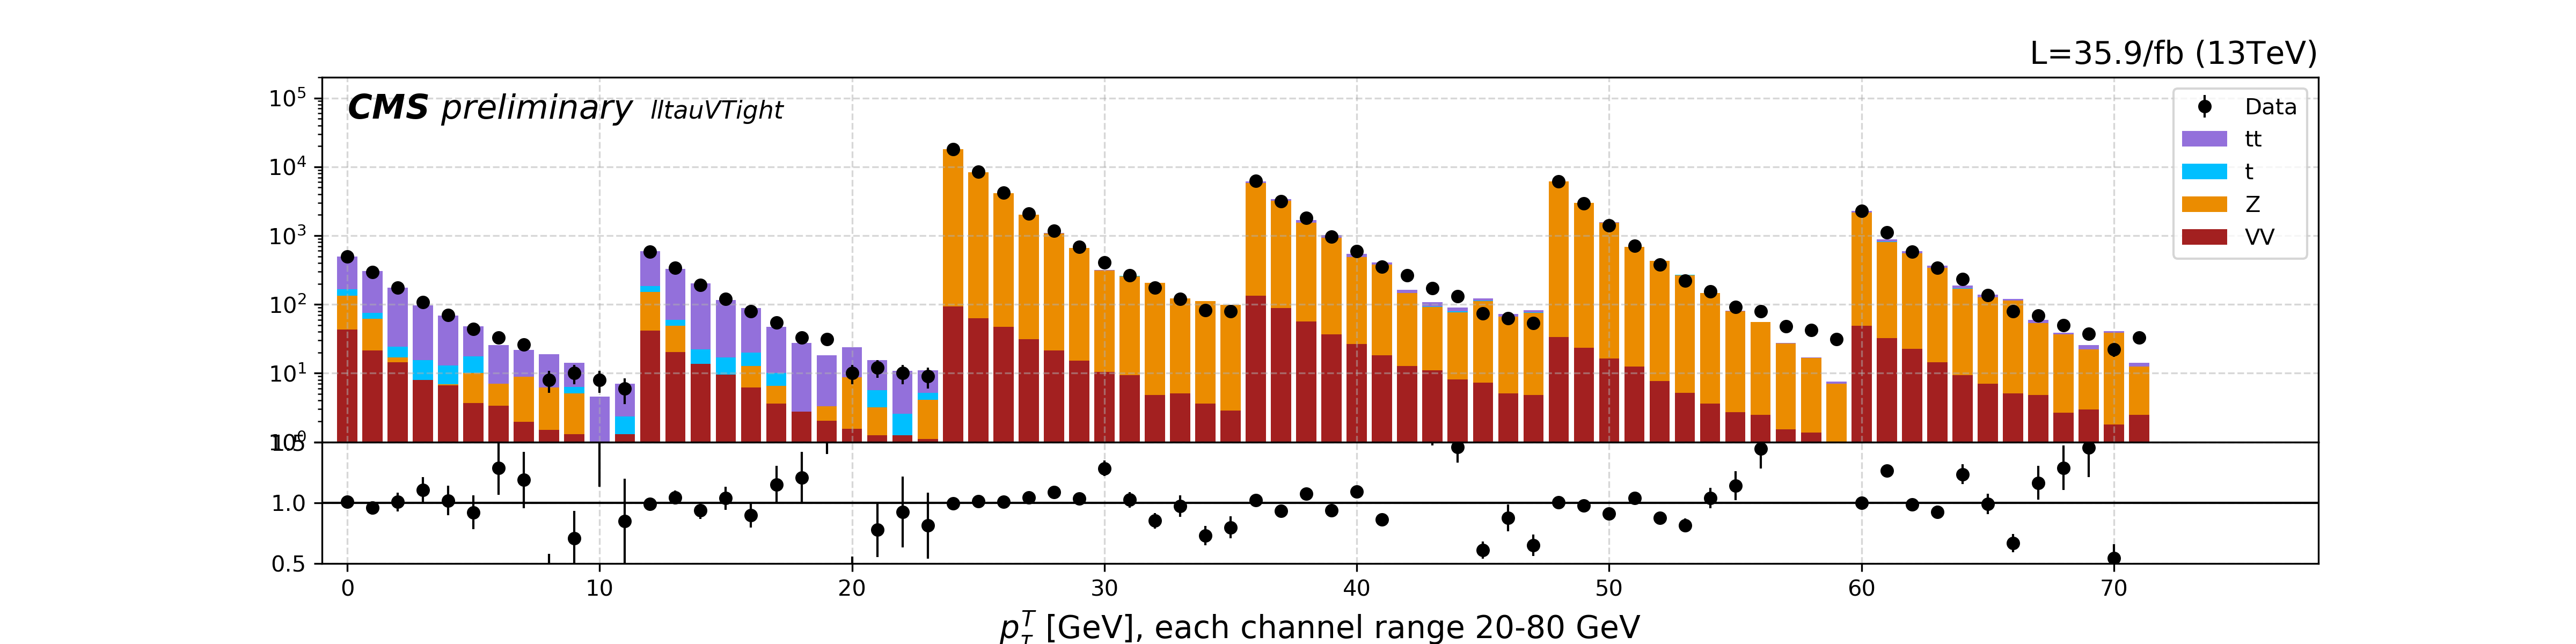
\includegraphics[width=0.99\textwidth]{chapters/Analysis/sectionCalibration/figures/jetToTauh/2020_tauID_postfit_lltauVTight.png}
%     \caption{Post distributions of $\tau_h$ \pt. Upper and lower are the Tight and VTight WP. }
%     \label{fig:appendix:fakeTauId:postfit}
% \end{figure}




To measure $SF (q\to \tau_h)$  and $SF (b\to \tau_h)$, a template fit to the $\tau_h$ \pt is performed.   The free parameters are $SF (q\to \tau_h)$  and $SF (b\to \tau_h)$ in 5 \pt bins from 20-80 GeV.  The systematical uncertainties, including cross sections, luminosity, electron/muon efficiency, are taken into account as nuisance parameters in the fit.



% \subsection{Result of the Scale Factors}



\begin{figure}
    \centering
    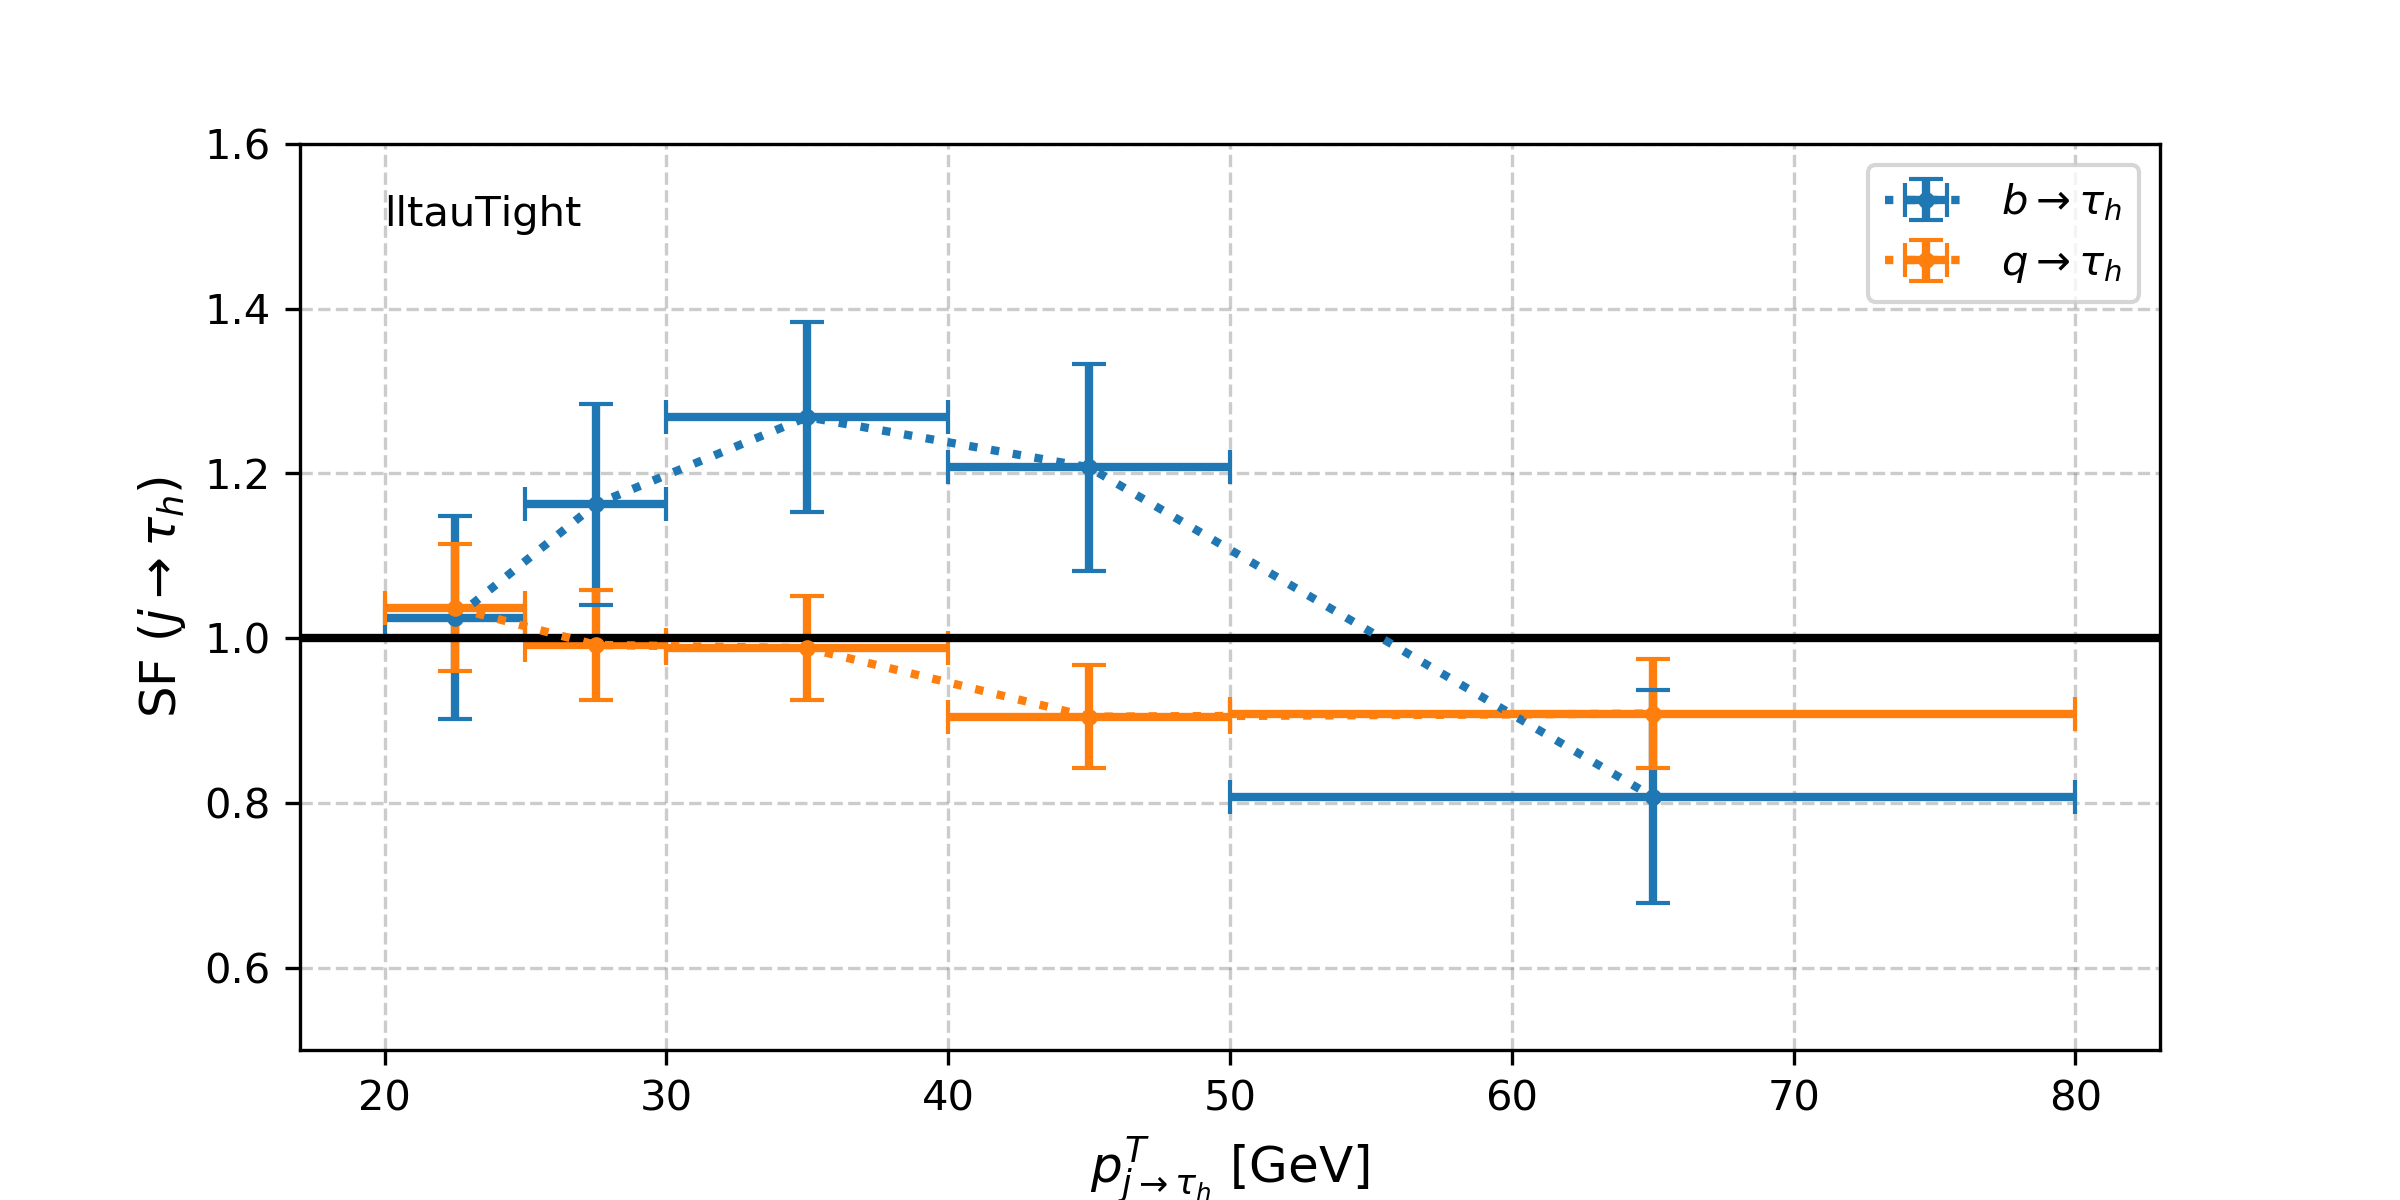
\includegraphics[width=0.49\textwidth]{chapters/Analysis/sectionCalibration/figures/jetToTauh/fit2_ptflavor2_lltauTight.png}
    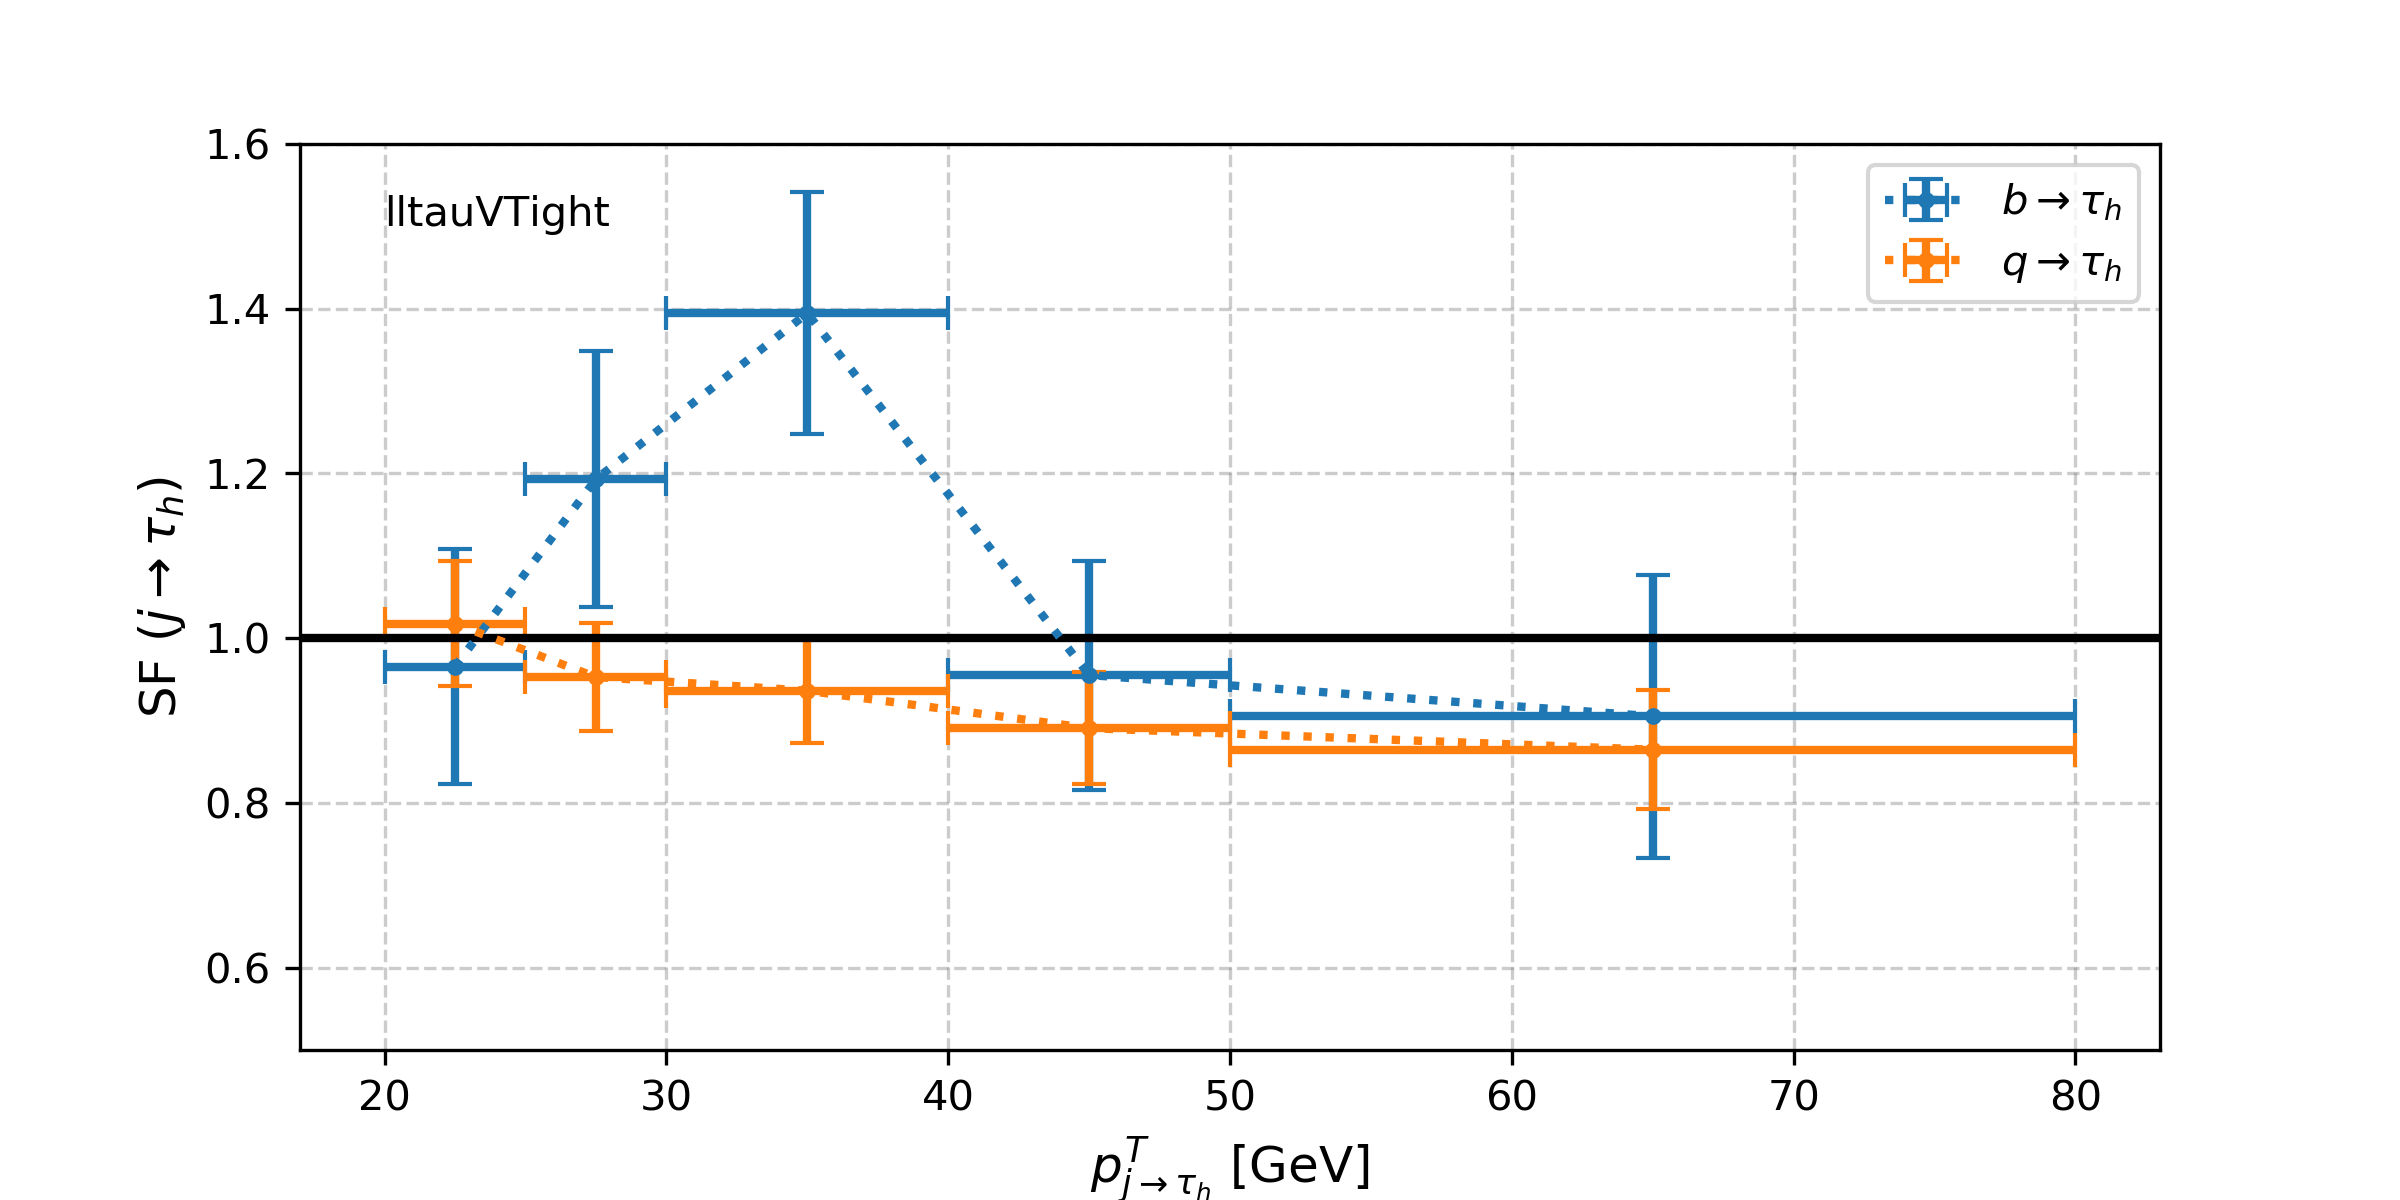
\includegraphics[width=0.49\textwidth]{chapters/Analysis/sectionCalibration/figures/jetToTauh/fit2_ptflavor2_lltauVTight.png}
    \caption{$SF (j\to \tau_h)$ for Tight and VTight tau.}
    \label{fig:appendix:fakeTauId:fit}
\end{figure}



The result of $SF (j\to \tau_h)$ for Tight and VTight WP are shown in figure~\ref{fig:appendix:fakeTauId:fit} and table~\ref{tab:appendix:fakeTauId:fit} The pulls and correlation matrix of the template fit are shown in Figure~\ref{fig:appendix:fakeTauId:fitparam}

In shape analysis, the uncertainty of $SF (j \to \tau_h)$ will be used as prefit uncertainty of the corresponding nuisance parameters.  In counting analysis,  the measured $SF (j \to \tau_h)$ will be variate according to the measured uncertainties.




\begin{figure}
    \centering
    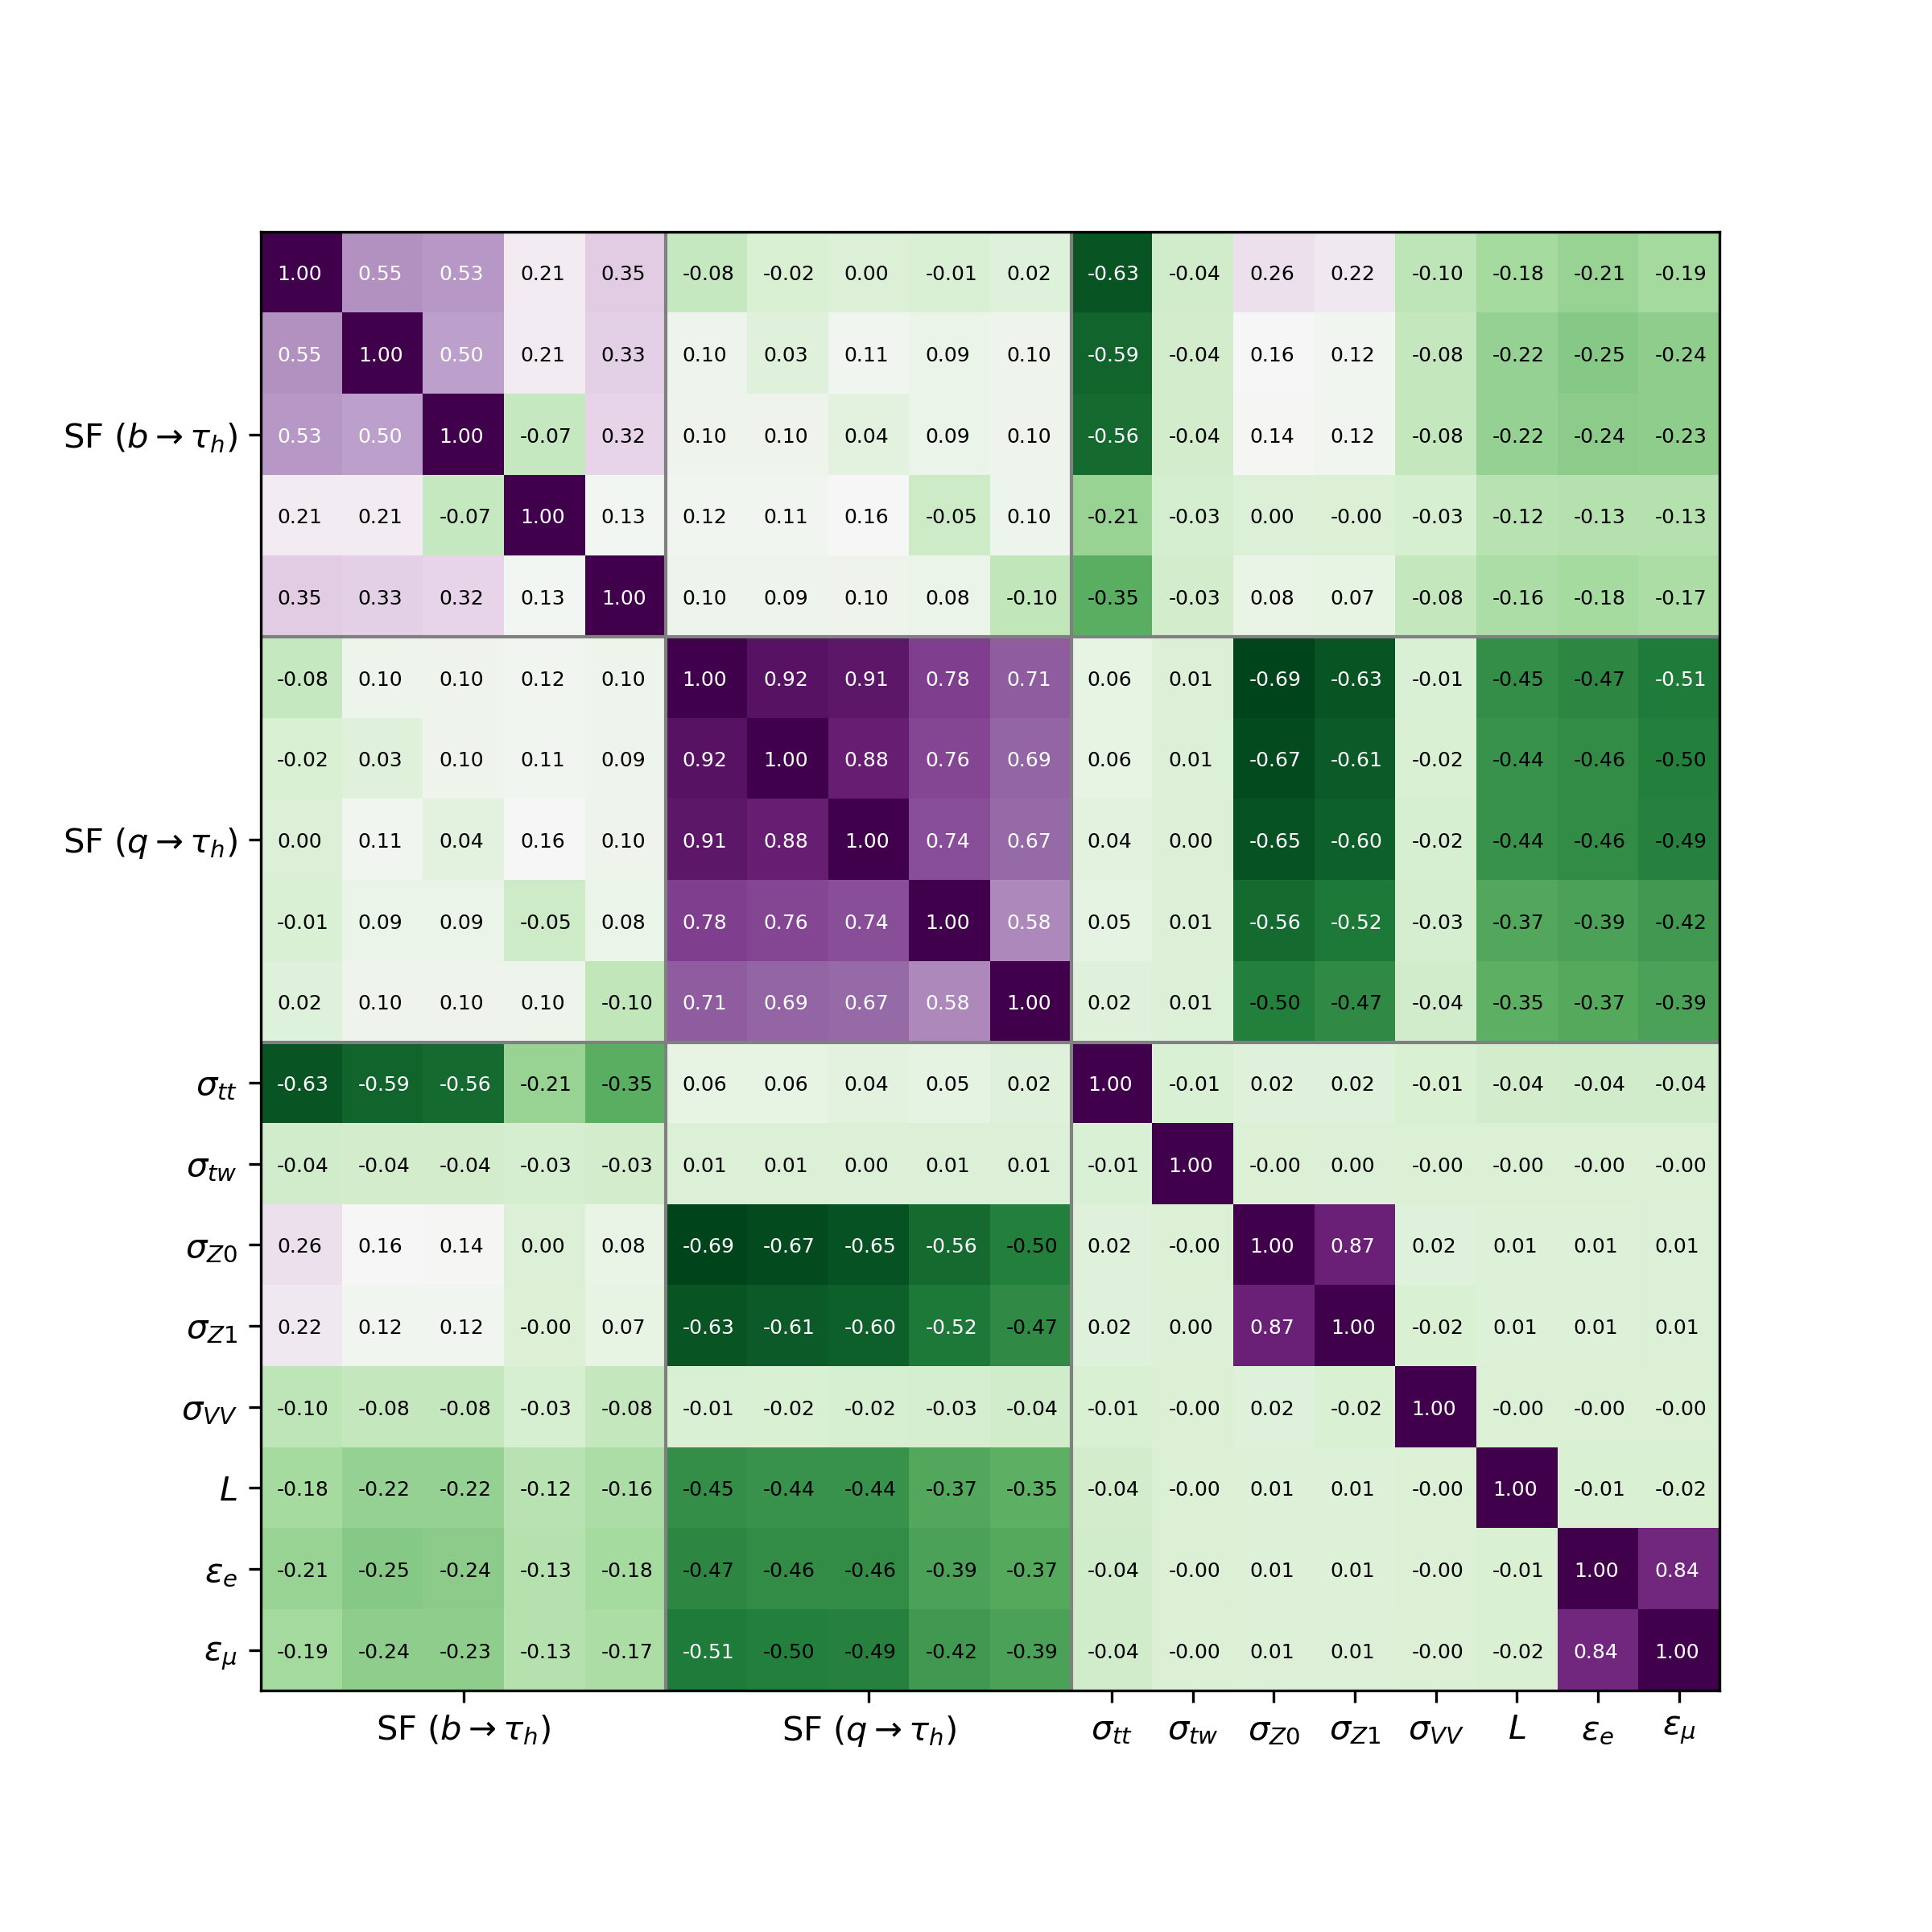
\includegraphics[width=0.49\textwidth]{chapters/Analysis/sectionCalibration/figures/jetToTauh/corr2_lltauTight_splitJetFlavor.png}
    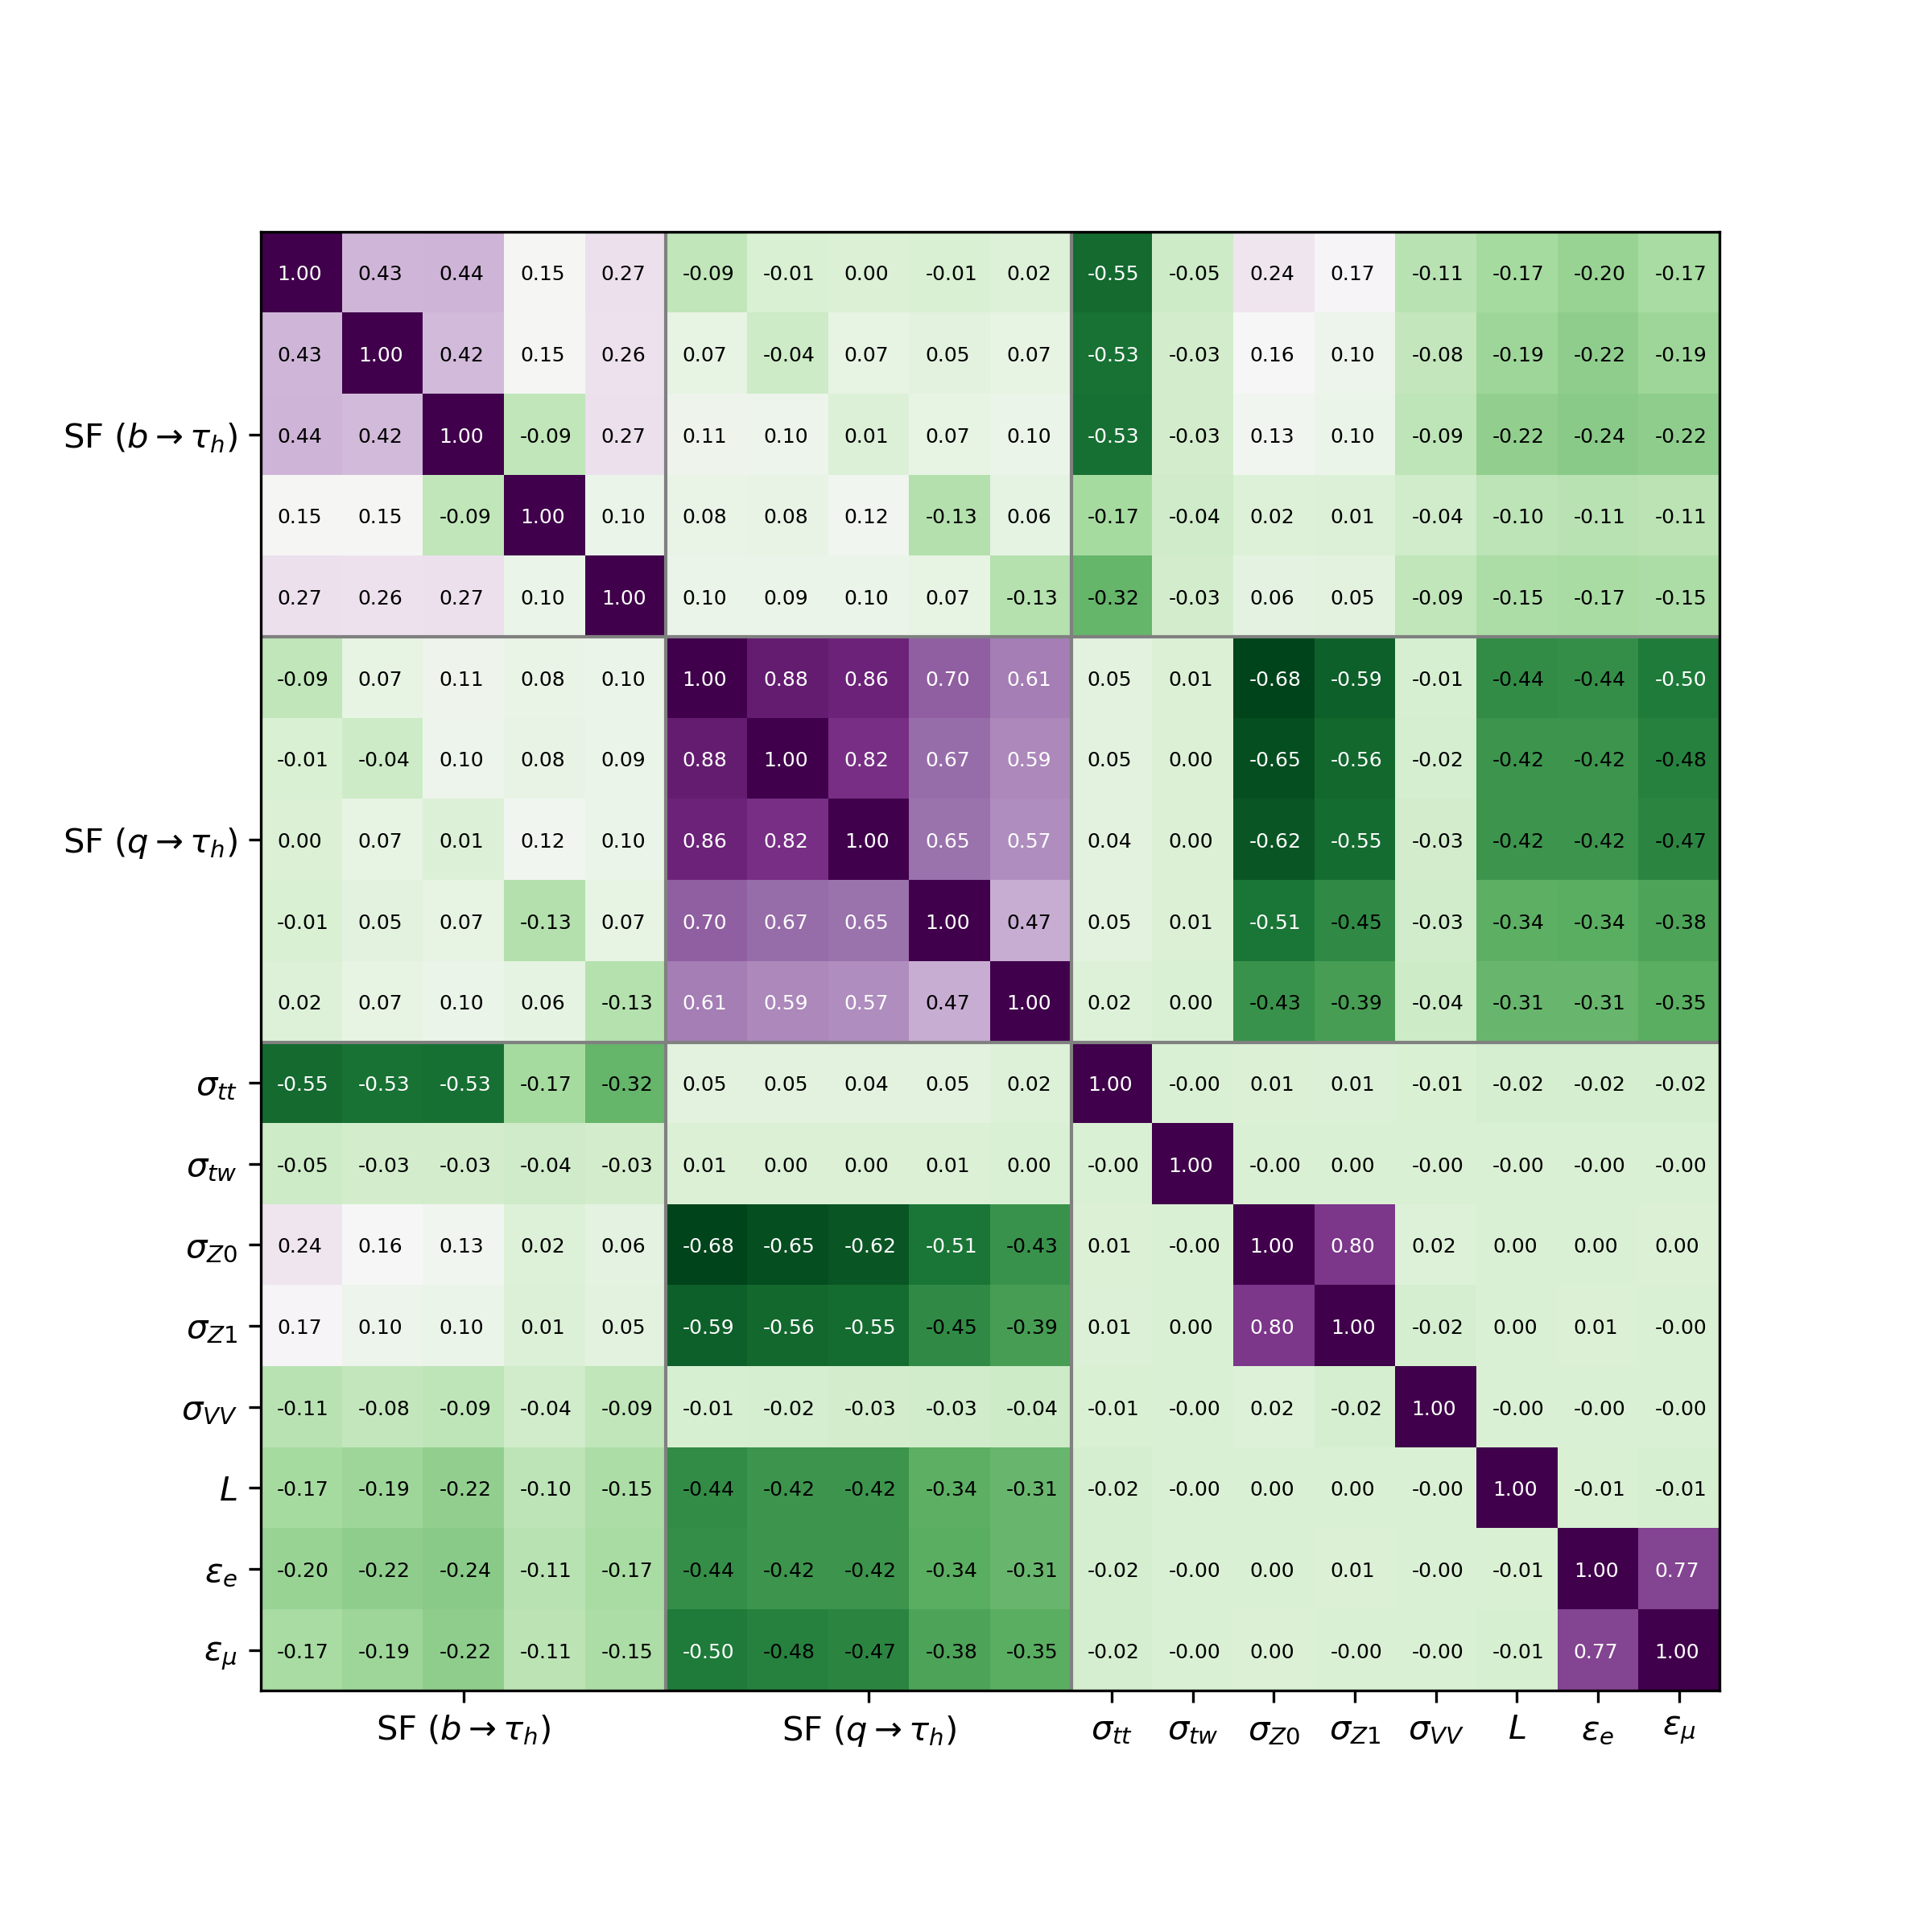
\includegraphics[width=0.49\textwidth]{chapters/Analysis/sectionCalibration/figures/jetToTauh/corr2_lltauVTight_splitJetFlavor.png}
    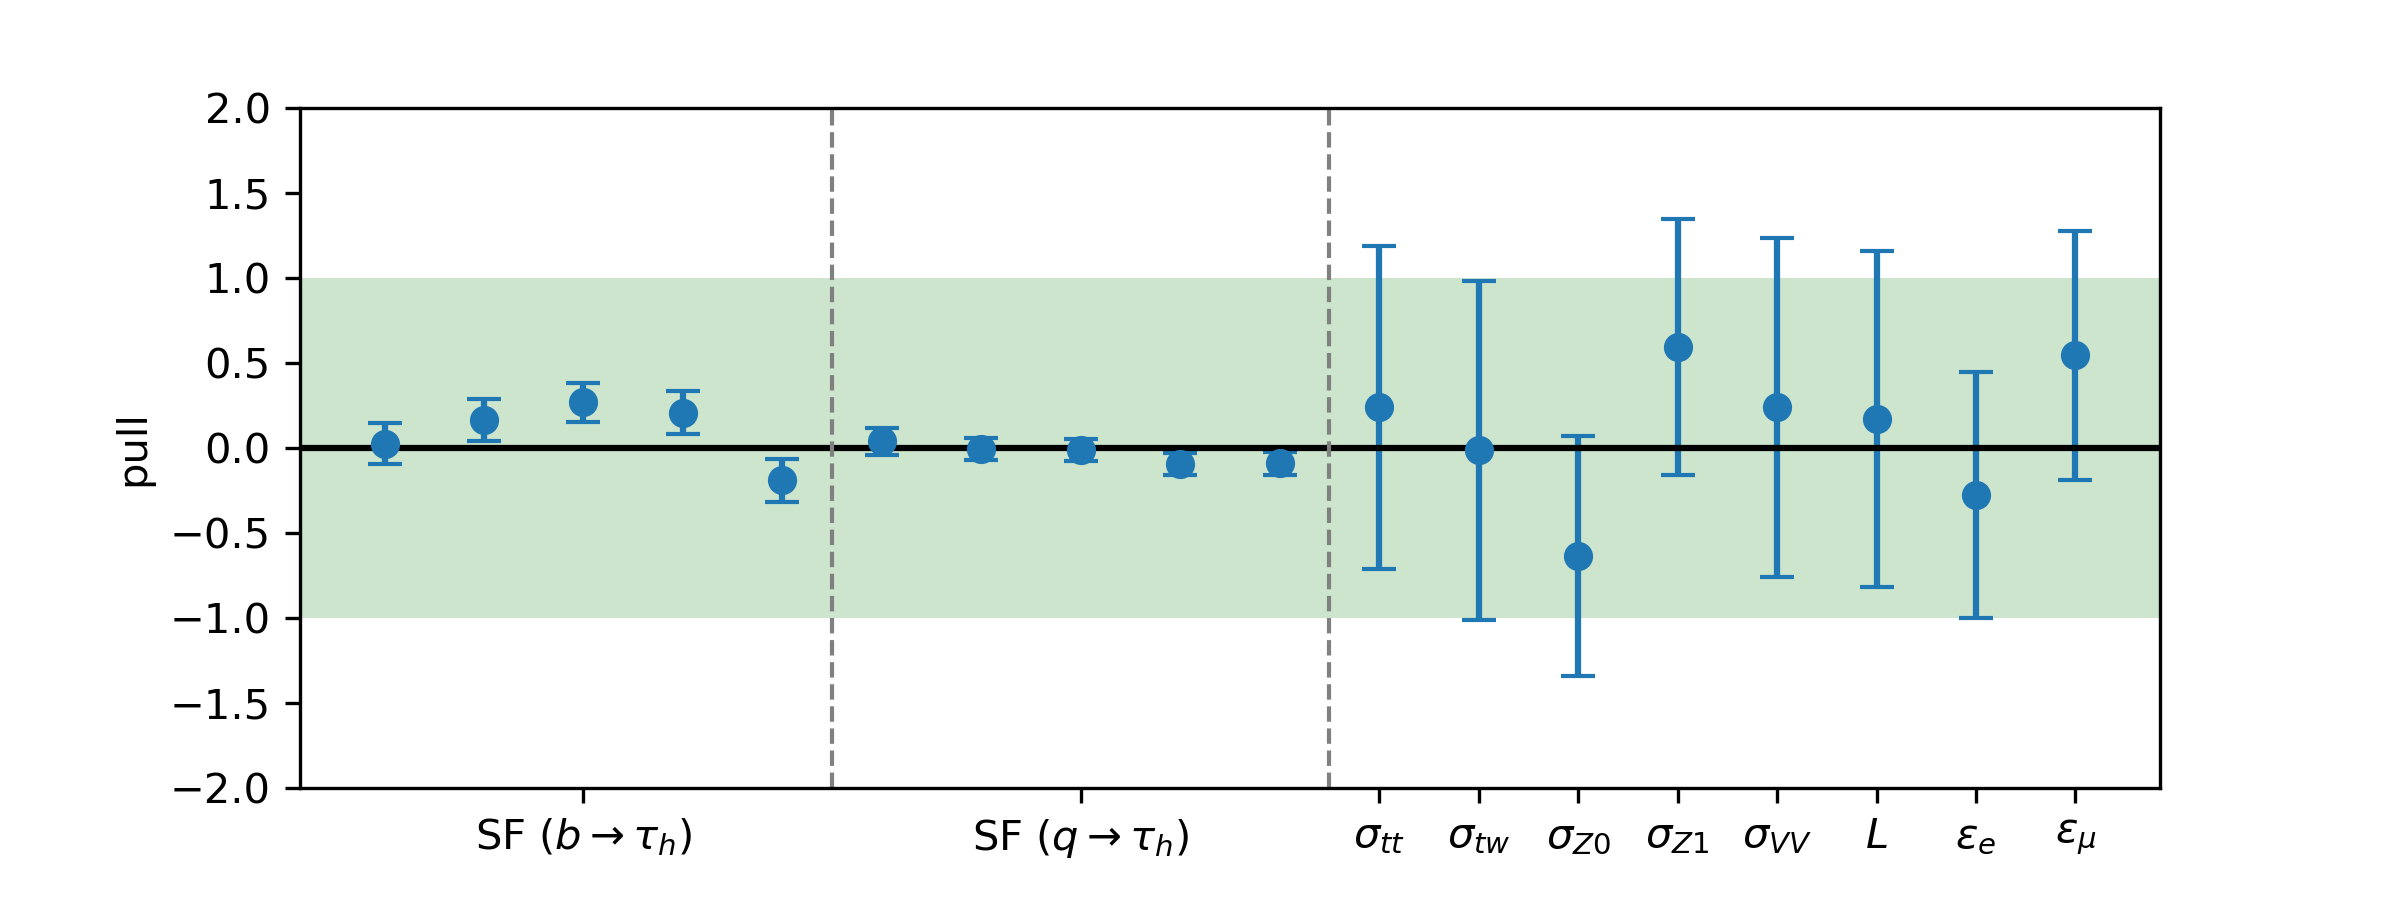
\includegraphics[width=0.49\textwidth]{chapters/Analysis/sectionCalibration/figures/jetToTauh/pull2_lltauTight_splitJetFlavor.png}
    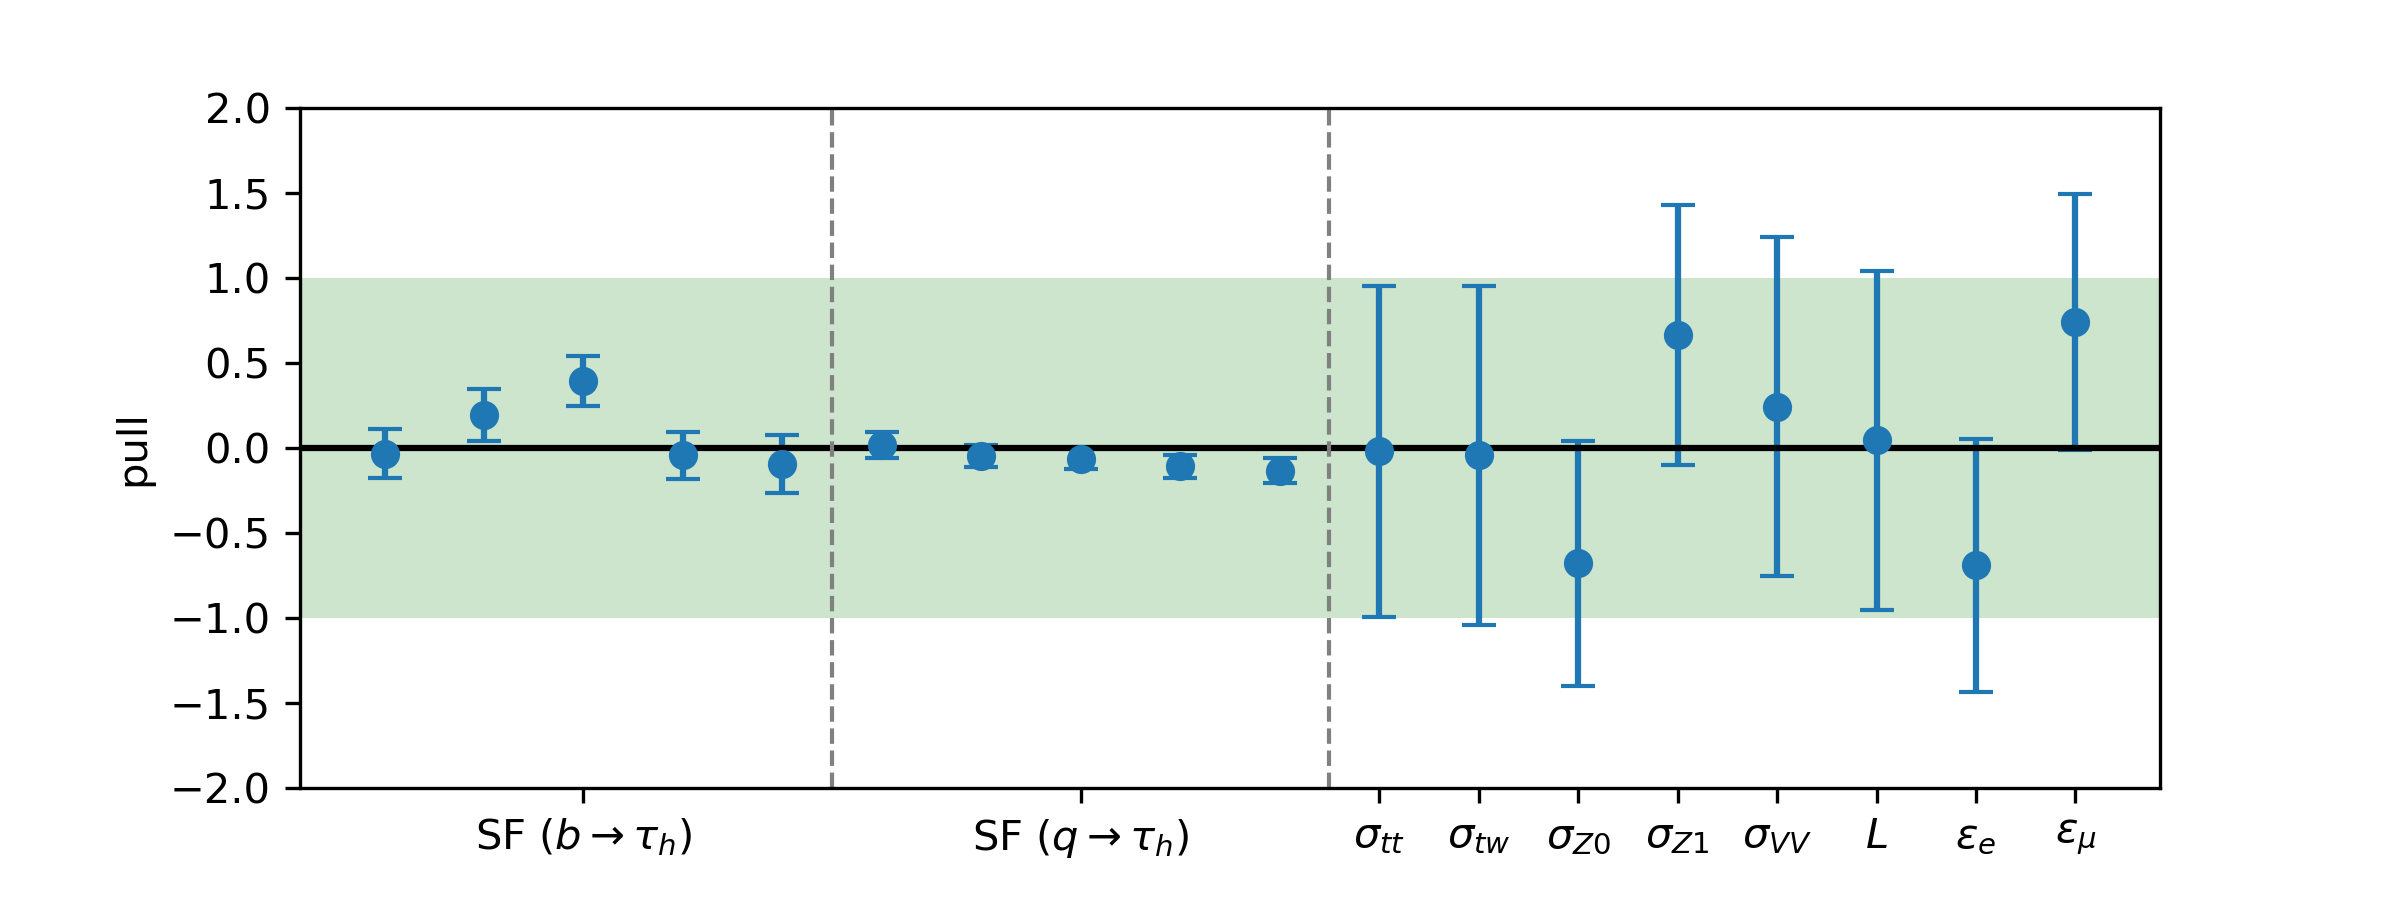
\includegraphics[width=0.49\textwidth]{chapters/Analysis/sectionCalibration/figures/jetToTauh/pull2_lltauVTight_splitJetFlavor.png}
    \caption{The correlation matrix and the pulls of the fitting parameters for Tight (left) and VTight (right) $\tau_h$. }
    \label{fig:appendix:fakeTauId:fitparam}
\end{figure}



\begin{table}[h]
    \setlength{\tabcolsep}{6pt} % Default value: 6pt
    \renewcommand{\arraystretch}{1.5} % Default value: 1
    \caption{ $SF (j\to \tau_h)$ for Tight and VTight tau.}
    
    \begin{tabular}{c|ccccc}
    \hline
    $p^T_{\tau_h}$ [GeV]  & 20-25         & 25-30         & 30-40         & 40-50         & 50-80         \\
    \hline
    $SF(b\to \rm{Tight} \; \tau_h)$  & $1.02\pm0.12$ & $1.16\pm0.12$ & $1.27\pm0.11$ & $1.21\pm0.13$ & $0.81\pm0.13$ \\
    $SF(q\to \rm{Tight} \;  \tau_h)$  & $1.04\pm0.08$ & $0.99\pm0.07$ & $0.99\pm0.06$ & $0.90\pm0.06$ & $0.91\pm0.07$ \\
    \hline
    $SF(b\to \rm{VTight} \; \tau_h)$ & $0.97\pm0.14$ & $1.19\pm0.16$ & $1.39\pm0.15$ & $0.96\pm0.14$ & $0.91\pm0.17$ \\
    $SF(q\to \rm{VTight} \; \tau_h)$ & $1.02\pm0.08$ & $0.95\pm0.07$ & $0.94\pm0.06$ & $0.89\pm0.07$ & $0.86\pm0.07$ \\
    \hline
    \end{tabular}
 
    \label{tab:appendix:fakeTauId:fit}
\end{table}


\FloatBarrier




\subsection{Measurement of b-tag Efficiencies in Simulation}
\label{sec:analysis:calibration:btag}


% \subsection{Corrections for b-tag Efficiencies}


To account for differences of the b-tag efficiency in data and simulation, a method that modifies the b-tag status of a jet is adopted in the simulation. In the method, the status is modified based on a set of data-to-simulation scale factors derived by the b-tag POG, and the efficiencies for simulation which have been measured independently in this section.  The method of the b-tag correction for simulation works as follows:

\begin{itemize}

    \item jets are identified as originating from the decay of a b quark, c quark, or ``light" parton (usdg) from generator truth information. Depending on the parton flavor and jet \pt, the appropriate scale factor $f_{\epsilon}$ and efficiency from simulation $\epsilon$ are looked up from a map.
    
    \item if $f_{\epsilon} < 1$, then a b-tagged jet is downgraded to a non-b tagged jet with probability,
        \begin{equation}
            p = 1 - f_{\epsilon}.
        \end{equation}
        \noindent if it is not b-tagged, nothing is changed.
    
    
    \item if $f_{\epsilon} > 1$, then a non-b-tagged jet is upgraded to a b-tagged jet with probability,
        \begin{equation}
            p = \frac{1 - f_{\epsilon}}{1 - \frac{1}{\epsilon}}.
        \end{equation}
        \noindent If it is already b-tagged, its status is unchanged.
\end{itemize}

% \subsection{b-tag Efficiencies in the Simulation}

Measurement of the b-tag efficiency in simulation relies on knowing the flavor of the parton that gives rise to the jet.  This is done with official CMS tools that assign a jet flavor based on the characteristics of the quark and gluon content of a jet~\cite{twiki:jet_mc_flavor}.  The efficiencies are measured for the case of b, c, and light (usdg) flavor jets, and as a function of the jet \pt.  That is,
\begin{equation}
    \epsilon(\pt, \mathrm{flavor}) = \frac{ N_{\mathrm{pass}}(\pt, \mathrm{flavor})} {N(\pt, \mathrm{flavor})},
\end{equation}

\noindent where the numerator is the number of jets passing the b-tag working point, and the denominator is the total number of jets considered. These quantities are measured in both \ttbar and \PZ plus jet samples. The CSVv2 discriminator value for the two samples are shown in figures~\ref{fig:btag_csvv2} for the three jet flavor categories. The efficiency measurement uses the middle working point of CSVv2 discriminator, the same as the selection in the measurement of \PW branching fraction. The result of b-tagging efficiencies is shown in figure~\ref{fig:btag_eff}.  There is some level of disagreement between the two samples for the b quark jets that likely could be attributed to the \ttbar sample being generated with an NLO generator (\POWHEG) and the \PZ plus jet sample being generated with a LO generator (\MADGRAPH). The efficiencies from \ttbar sample is used for the b-tag correction. The events used for the selection require at least muon passing our analysis requirements, and the four leading \pt jets are considered in the measurement.

\begin{figure}[h!]
    \centering
    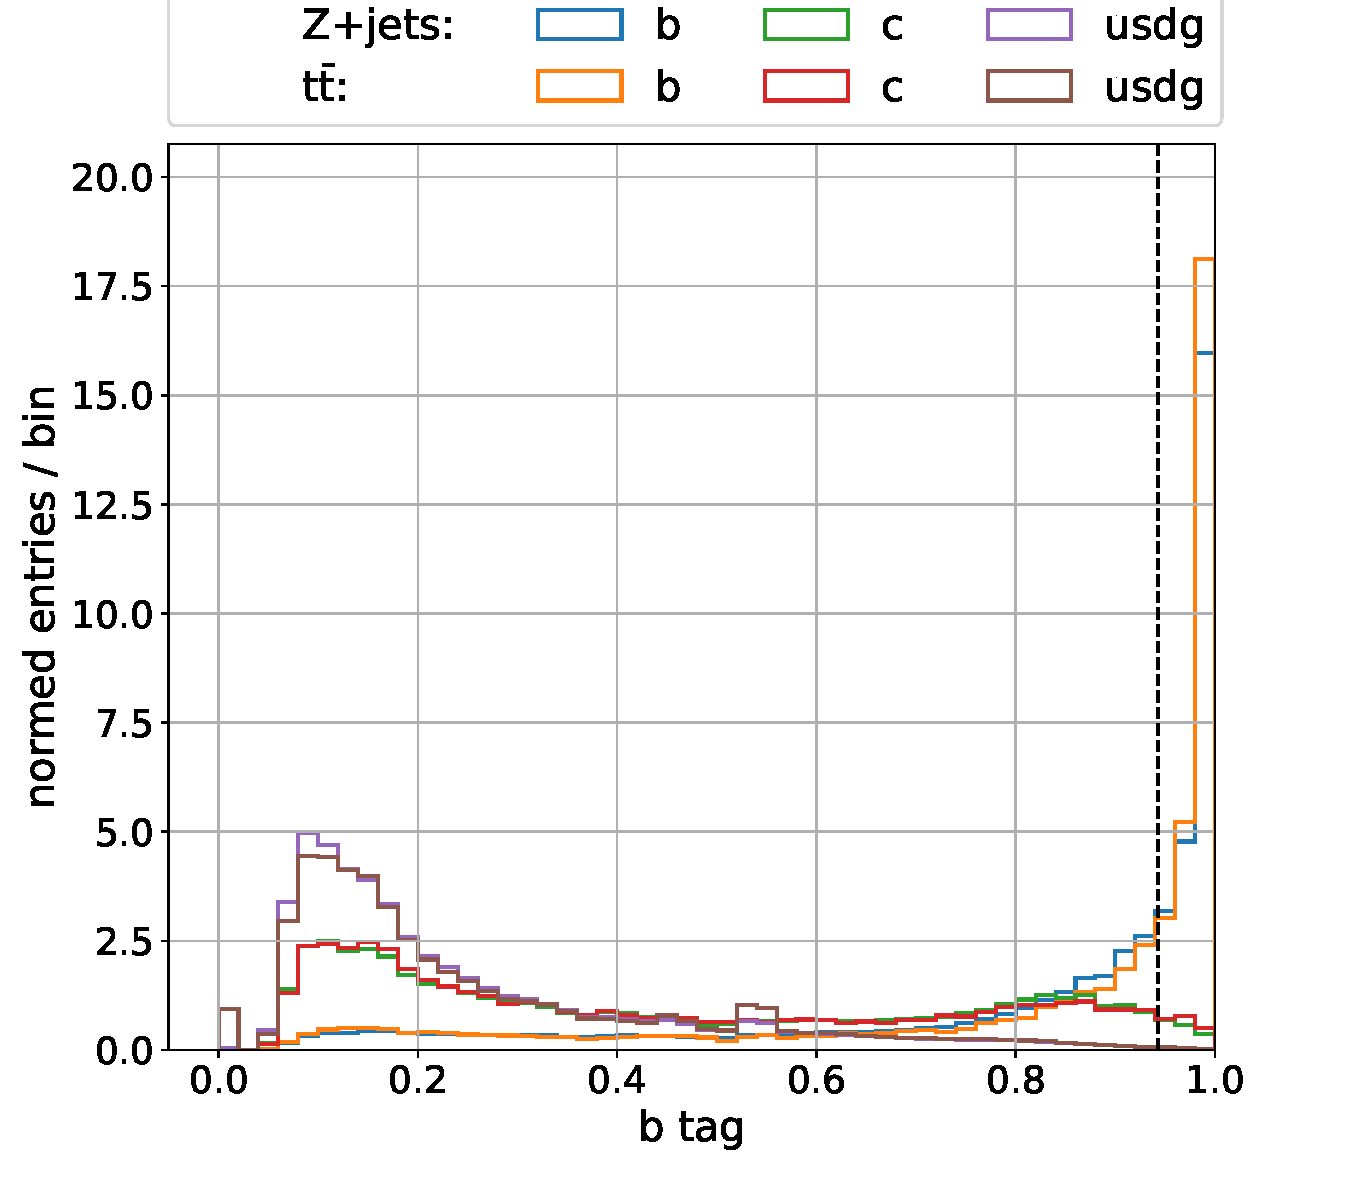
\includegraphics[width=0.45\textwidth]{chapters/Analysis/sectionCalibration/figures/btag/bmva_mc.pdf}
    \caption{Distribution of ``csv" b-tag discriminator for the three flavor categories under consideration for \PZ + jet and \ttbar events.      
    \label{fig:btag_csvv2}}
\end{figure}

\begin{figure}[h!]
    \centering
    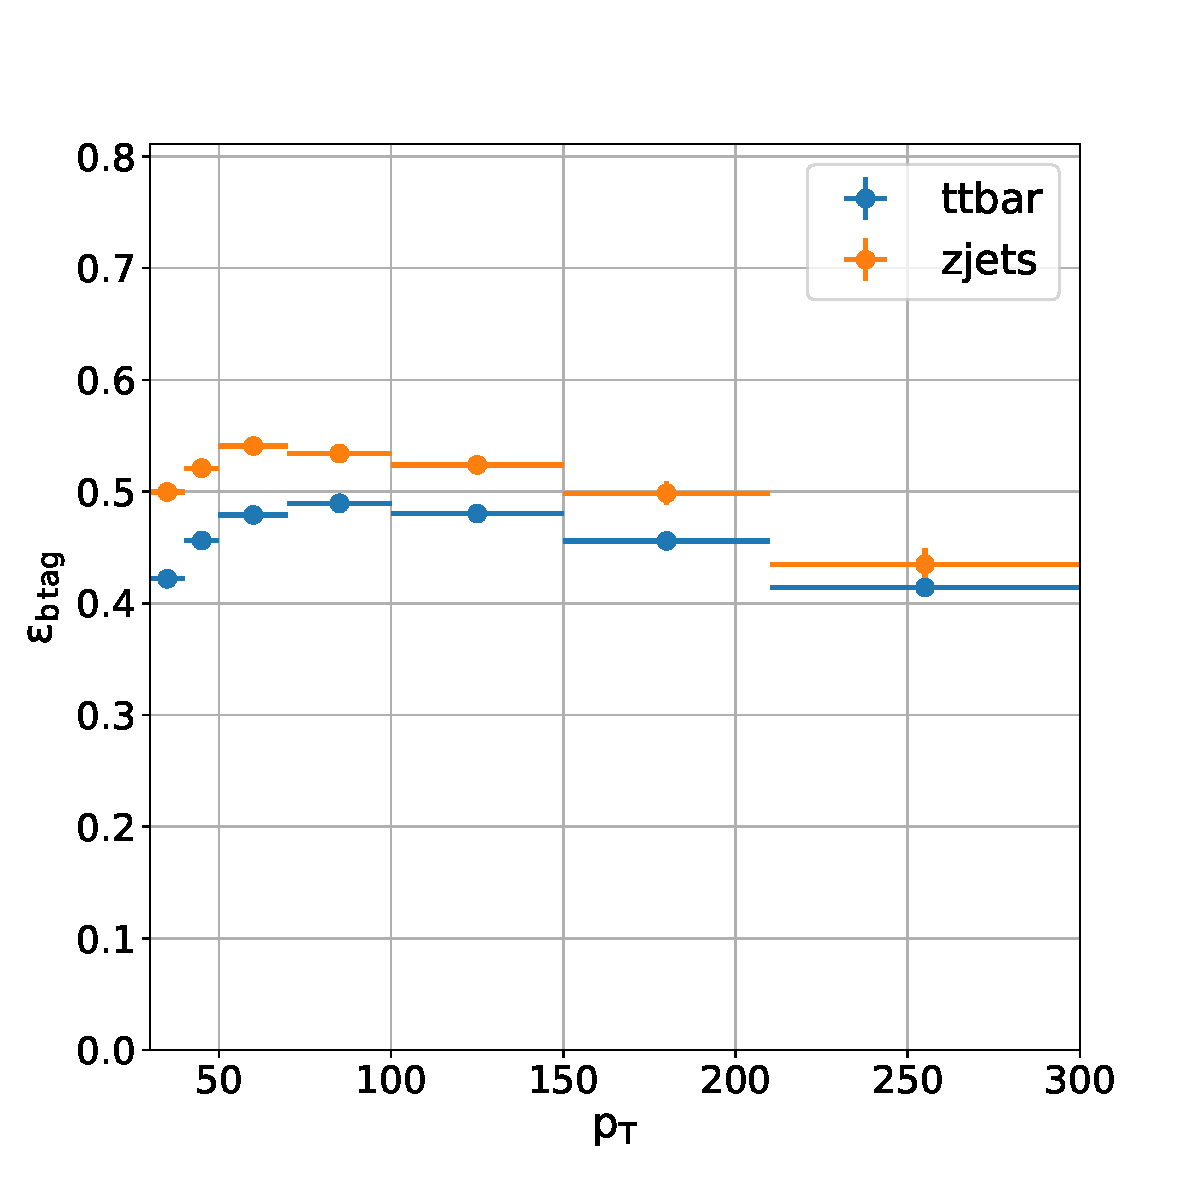
\includegraphics[width=0.3\textwidth]{chapters/Analysis/sectionCalibration/figures/btag/bmva_mceff_vs_pt_b}
    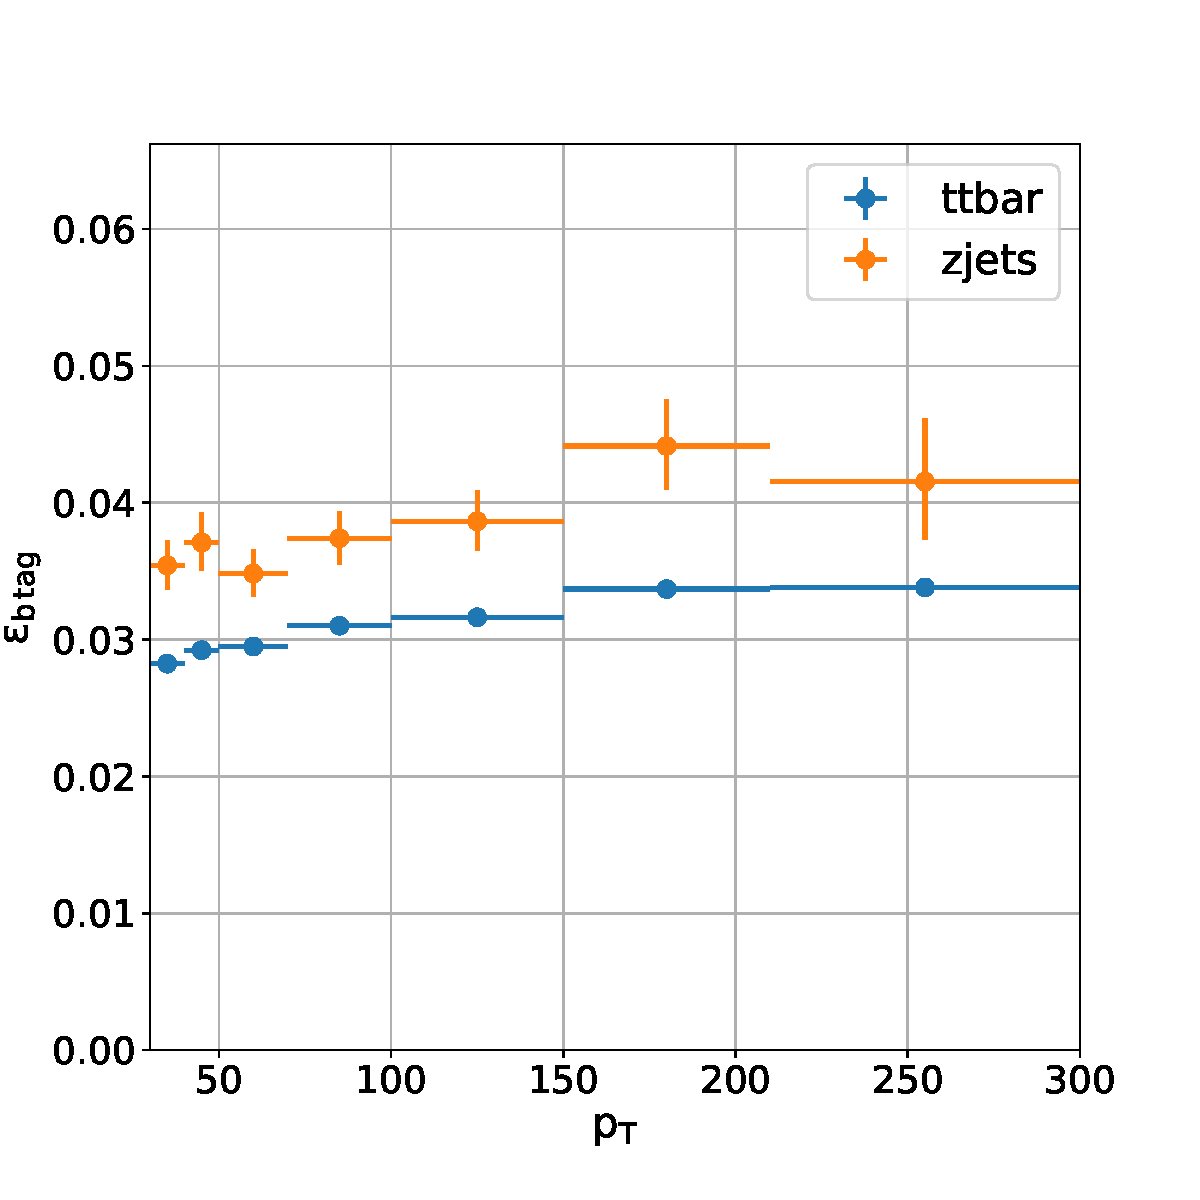
\includegraphics[width=0.3\textwidth]{chapters/Analysis/sectionCalibration/figures/btag/bmva_mceff_vs_pt_c}
    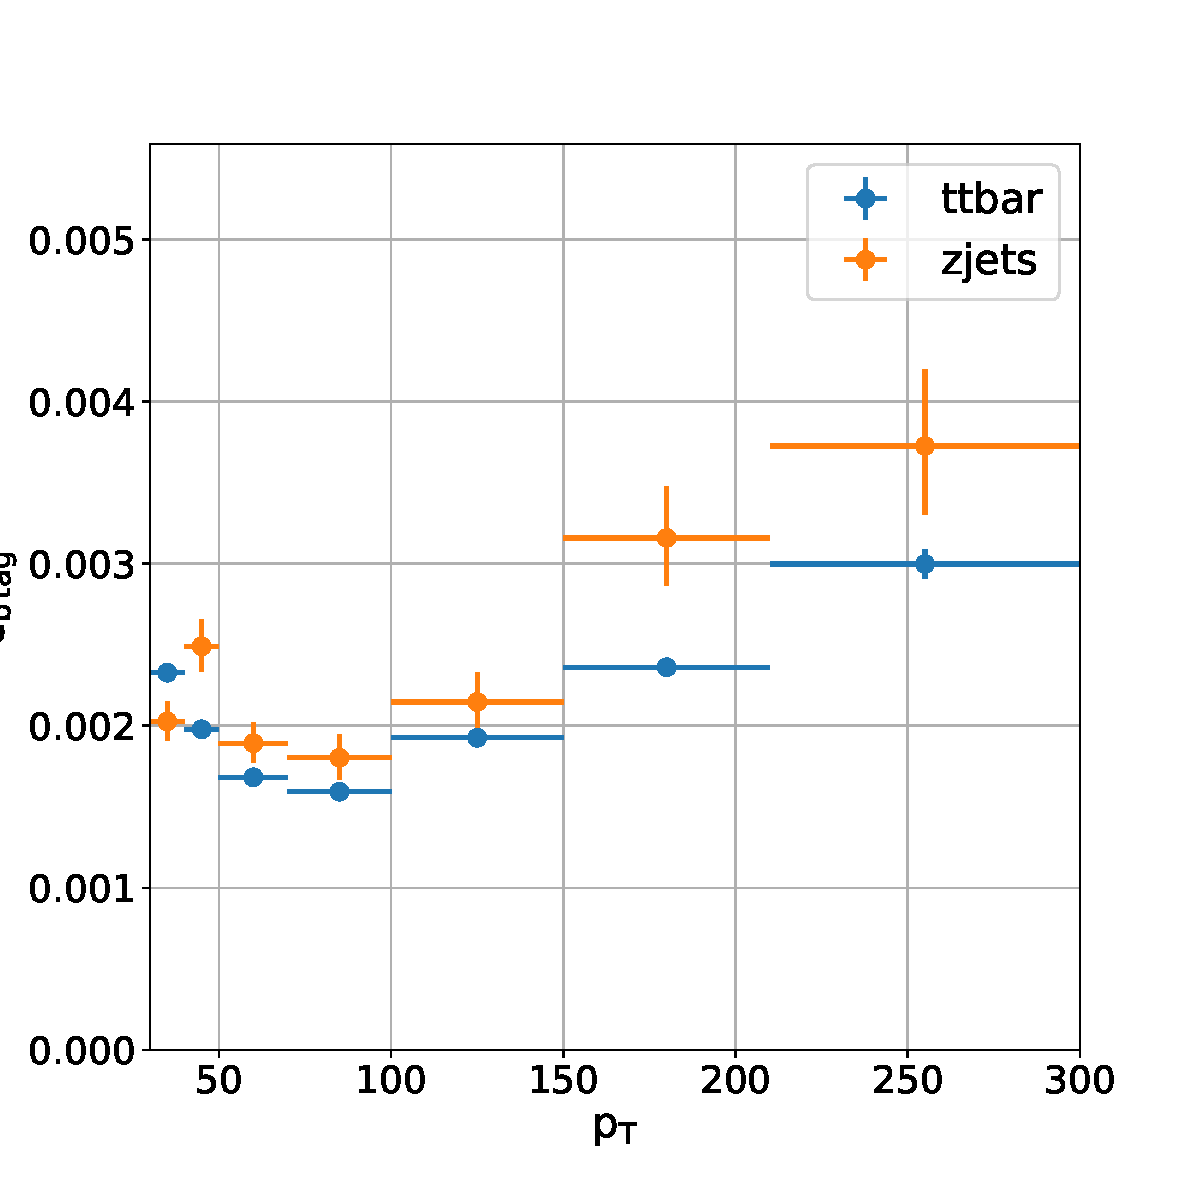
\includegraphics[width=0.3\textwidth]{chapters/Analysis/sectionCalibration/figures/btag/bmva_mceff_vs_pt_usdg}
    \caption{Efficiency to b-tag a jet originating from a b quark (left), c quark (middle), and light quark (right).
    \label{fig:btag_eff}
    }
\end{figure}

\FloatBarrier





\subsection{Reweight of Different Hadronic Tau Decay Modes in the Simulation}
\label{sec:analysis:calibration:tauBr}

The MC events with $\tau_h$ in the $e\tau$ and $\mu \tau$ channel is essential to the sensitivity of the $Br(W\to\tau)$ measurement. However, the tau's hadronic decay branching fraction $B(\tau \to  \rm{hadrons})$ in the MC simulation are different from the experimental world average in the PDG. The $\tau_h$ selection efficiency could be impacted by such difference because various tau's hadronic  decay mode have different efficiencies in the CMS $\tau_h$ reconstruction with SPH algorithm.

Thus it is necessary to reweight the MC events to correct the deviation of tau's decay in the simulation with respect to the PDG values. For the values in the \PYTHIA simulation assumption and the PDG world average, tau's hadronic decay branching fractions are listed in table~\ref{tab:tauhReweighting}. The difference between values in \PYTHIA8 and PDG is about $0.5\%$. The ratios of PDG and \PYTHIA values are also included, which are the event weights applied for the $\tau \to h$ reweighting.

    
    
\begin{table}[ht]
  \centering
  \setlength{\tabcolsep}{1 em}
  \renewcommand{\arraystretch}{1.5}
  \caption{ The values of $B(\tau \to  \rm{hadrons})$ in PYTHIA8 and in PDG.}
  \begin{tabular}{l|c|c|c}
  \hline
                              & PDG        & \PYTHIA   & PDG / \PYTHIA \\
  \hline
  $B(\tau\to \pi^\pm)$       & 0.1082(5)  & 0.1076825 & 1.00481       \\
  $B(\tau\to \pi^\pm+ \pi^0)$& 0.2549(9)  & 0.2537447 & 1.00455       \\
  $B(\tau\to \pi^\pm+2\pi^0)$& 0.0926(10) & 0.0924697 & 1.00141       \\
  $B(\tau\to3\pi^\pm)$       & 0.0931(5)  & 0.0925691 & 1.00574       \\
  $B(\tau\to3\pi^\pm+ \pi^0)$& 0.0462(5)  & 0.0459365 & 1.00574       \\
  \hline
  \end{tabular}
  \label{tab:tauhReweighting}
\end{table}


\begin{figure}
    \centering
    \includegraphics[width=0.99\textwidth]{chapters/Analysis/sectionCalibration/figures/tauBr/tauhDecay_mutau.png}
    \includegraphics[width=0.99\textwidth]{chapters/Analysis/sectionCalibration/figures/tauBr/tauhDecay_mutau2.png}
    \includegraphics[width=0.99\textwidth]{chapters/Analysis/sectionCalibration/figures/tauBr/tauhDecay_etau.png}
    \includegraphics[width=0.99\textwidth]{chapters/Analysis/sectionCalibration/figures/tauBr/tauhDecay_etau2.png}
    \caption{The gen-level daughter mesons from hadronicly decaying taus in the $tt\to \mu \tau_h, e \tau_h$ events passing $\mu \tau$ and $e \tau$ selection.}
    \label{fig:appendix:reweightTauhBr:tauhBr}
\end{figure}


In MC events, the gen-level daughter mesons from hadronically decaying taus are saved.  The $\tau_h$'s daughter mesons in the $tt\to \mu \tau_h, e \tau_h$ events  passing $\mu \tau$ and $e \tau$ selection are shown in Fig~\ref{fig:appendix:reweightTauhBr:tauhBr} The leading contributions to the reconstructed $\tau_h$ are $\tau\to \pi^\pm+\pi^0 $, $\tau\to 3\pi^\pm$, $\tau\to \pi^\pm+2\pi^0$, $\tau\to \pi^\pm$, $\tau\to 3\pi^\pm + \pi^0$.  MC events with taus in those five decay modes are reweighted by 

\begin{equation}
  w = \frac{^{\rm PDG} B(\tau \to  \rm{hadrons}) }{^{\rm \PYTHIA} B( \tau \to \rm{hadrons} )}. 
\end{equation} 


\noindent The uncertainties of the weights are from the the PDG uncertainties.  The systematical uncertainty due to the uncertainties of $B(\tau \to  \rm{hadrons})$ reweighting can be estimated. The effect of the $B(\tau \to  \rm{hadrons})$  reweighting on the $B(W)$ result is small. The relative systematics from $B(\tau \to  \rm{hadrons})$ reweighting are about $0.003 - 0.146 \%$,  shown in table~ \ref{tab:syst_tauhReweighting}.



\begin{table}[p]
  \centering
  \caption{ Relative systematic uncertainty ($\%$) due to $B(\tau \to  \rm{hadrons})$ reweighting.}
  \setlength{\tabcolsep}{0.5 em}
  \renewcommand{\arraystretch}{2}
  \resizebox{\textwidth}{!}{
  \begin{tabular}{|l|ccc|ccc|ccc|ccc|ccc|}
    \hline
    Error Source & \multicolumn{3}{c|}{$\mu$-1b} & \multicolumn{3}{c|}{$\mu$-2b} & \multicolumn{3}{c|}{$e$-1b} & \multicolumn{3}{c|}{$e$-2b} \\
    \hline
                  & $B_e$ & $B_\mu$ & $B_\tau$ & $B_e$ & $B_\mu$ & $B_\tau$ & $B_e$ & $B_\mu$ & $B_\tau$ & $B_e$ & $B_\mu$ & $B_\tau$ \\
    \hline
    0.5$\%$ err of $Br_{\tau\to\pi^\pm}$       & 0.009 & 0.013 & 0.055 & 0.009 & 0.012 & 0.051 & 0.009 & 0.012 & 0.052 & 0.010 & 0.012 & 0.057 \\ 
    0.5$\%$ err of $Br_{\tau\to\pi^\pm\pi^0}$  & 0.025 & 0.033 & 0.141 & 0.026 & 0.033 & 0.147 & 0.024 & 0.032 & 0.146 & 0.025 & 0.032 & 0.146 \\ 
    0.2$\%$ err of $Br_{\tau\to\pi^\pm2\pi^0}$ & 0.003 & 0.004 & 0.017 & 0.003 & 0.004 & 0.015 & 0.003 & 0.004 & 0.017 & 0.003 & 0.004 & 0.019 \\ 
    0.6$\%$ err of $Br_{\tau\to3\pi^\pm}$      & 0.017 & 0.022 & 0.101 & 0.019 & 0.023 & 0.111 & 0.017 & 0.023 & 0.107 & 0.017 & 0.022 & 0.107 \\ 
    0.6$\%$ err of $Br_{\tau\to3\pi^\pm\pi^0}$ & 0.005 & 0.006 & 0.024 & 0.005 & 0.006 & 0.022 & 0.004 & 0.006 & 0.022 & 0.005 & 0.006 & 0.025 \\ 
    \hline
  \end{tabular}}
  \label{tab:syst_tauhReweighting}
\end{table}
\FloatBarrier

\section{Background Estimation}
\label{sec:analysis:background}


The \BWl measurement has four sources of standard model backgrounds:

\begin{itemize}
    \item vector boson plus jets (\wjets in counting analysis, \zjets)
    \item photon plus jets (\gjets)
    \item diboson production ($\PW\PW$ in counting analysis, $\PZ\PZ$, $\PZ\PW$)
    \item multijet QCD
\end{itemize}

It is worth pointing out that the \wjets and $\PW\PW$ processes are treated as backgrounds in counting analysis, but the shape analysis treats them as signals. This is because the counting analysis uses only the \ttbar enriched signal region, while the shape analysis includes extra control regions with relaxed jet multiplicities requirement. Overall, vector boson plus jets are the most prominent source of backgrounds. The contributions from \gjets are much smaller and mainly in the \ceh channel. The contributions from diboson processes $\PW\PW$, $\PZ\PZ$, $\PZ\PW$ are even smaller. In the \ttbar regions, the contributions from these backgrounds are very small in comparison with the signals. The backgrounds from \zjets, \wjets, \gjets and diboson processes are all well modeled by the simulated datasets. Non-negligible contamination from QCD processes are found in \cet, \cmt, \ceh, \cmh channels. The \HT-binned QCD simulations are evaluated, and turn out to be statistically sufficient at an acceptable level for the normalization in the $\ceh$ and $\cmh$ channels which requires high jet multiplicities $n_j\geq 4$. However, the number of simulated QCD events is insufficient for accurately modelling shape of kinematics distributions. Therefore, data-driven approaches are employed to estimate the QCD background in the \cet, \cmt, \ceh, \cmh channels. For \cet, \cmt channel, a same-sign region is used. For \ceh, \cmh channel, the region with inverted lepton isolation is used.



\subsection{QCD background in the $e \tau_\mathrm{h}$ and $\mu \tau_\mathrm{h}$ channels}

This estimation relies on the dearth of standard model processes that can give rise to same-sign lepton pairs.  It is expected that most events with same-sign lepton pairs are the result of at least one of the leptons coming from non-prompt decays.  It is further assumed that this process will give rise to misidentifying hadronic jets as leptons in near equal measure between the same sign and opposite sign selections.  

The process of deriving the estimate is simple enough: requiring the electron or muon having the same sign as the hadronic tau in the \cet and \cmt channel. All other selection requirements are kept unchanged. The deficit between data and standard model simulation in the same-sign side-band region is multiplied by a transferring scale factor to estimate the QCD contamination in the signal region. 


The same-sign (SS) to opposite-sign (OS) transfer scale factor transfer factor is calculated by
\begin{equation}
    SF^{\rm SS \to OS} = \frac{N^{\rm OS}_{\rm data} - \sum N^{\rm OS}_{\rm MC} }{ N^{\rm SS}_{\rm data} - \sum N^{\rm SS}_{\rm MC} }
\end{equation}
\noindent To determine $SF^{\rm SS \to OS}$, the counting analysis uses \cet and \cmt channels with $n_j=2,n_\PQb=0$. The SS and OS regions of \cet and \cmt channels with different $n_j,n_\PQb$ configurations are shown in Figure~\ref{fig:background:ltau:mass_ltau_1} and \ref{fig:background:ltau:mass_ltau_2}. The $SF^{\rm SS \to OS}$ measured from $n_j=2,n_\PQb=0$ is chosen because the jet and \PQb tag configuration is closest to the signal region. The corresponding results of $SF^{\rm SS \to OS}$ are 1.062 and 1.195 for \cet and \cmt channel, respectively.



For shape analysis, this region is treated as a signal region. So the regions with anti-isolated electron or muon plus \PGth with $n_j=0$ are used to measure  $SF^{\rm SS \to OS}$. Figure~\ref{fig:background:ltau:mass_ltau_antiiso} shows the $m_{\cet}$ and $m_{\cmt}$ distributions distributions in the same-sign and opposite-sign regions of \cet (on the right) and \cmt (on the left) channel with the anti-isolated lepton and zero jets.

\begin{figure}[h]
    \centering
    \includegraphics[width=0.49\textwidth]{chapters/Analysis/sectionBackground/figures/ltau_kinematics/mutau_cr.pdf}
    \includegraphics[width=0.49\textwidth]{chapters/Analysis/sectionBackground/figures/ltau_kinematics/etau_cr.pdf}
    \caption{The $m_{\cet}$ and $m_{\cmt}$ distributions in the same-sign and opposite-sign regions of \cet (on the right) and \cmt (on the left) channel with the anti-isolated lepton and zero jets.}
    \label{fig:background:ltau:mass_ltau_antiiso}
\end{figure}

\begin{sidewaysfigure}[h]
    \centering
    \includegraphics[width=0.9\textwidth]{chapters/Analysis/sectionBackground/figures/ltau_kinematics/ltau1.png}
    \caption{The $m_{\cmt}$ distributions in the same-sign and opposite-sign regions of \cmt channel \emph{(left two columns)}. The $m_{\cet}$ spectrum in the same-sign and opposite-sign regions of \cet channel \emph{(right two columns)}. Three rows correspond to $n_j=0,n_\PQb=0$, $n_j=1,n_\PQb=0$, $n_j=1,n_\PQb=1$, respectively. }
    \label{fig:background:ltau:mass_ltau_1}
\end{sidewaysfigure}
\begin{sidewaysfigure}[h]
    \centering
    \includegraphics[width=0.9\textwidth]{chapters/Analysis/sectionBackground/figures/ltau_kinematics/ltau2.png}
    \caption{The $m_{\cmt}$ distributions in the same-sign and opposite-sign  regions of \cmt channel \emph{(left two columns)}. The $m_{\cet}$ spectrum in the same-sign and opposite-sign regions of \cet channel \emph{(right two columns)}. Three rows correspond to $n_j\geq 2,n_\PQb=0$, $n_j\geq 2,n_\PQb=1$, $n_j\geq 2,n_\PQb\geq 2$, respectively.}
    \label{fig:background:ltau:mass_ltau_2}
\end{sidewaysfigure}




\FloatBarrier





\subsection{QCD background in the $e\mathrm{h}$ and $\mu \mathrm{h}$ channels}

% A commonly used method for estimating backgrounds from misidentified prompt lepton production can be summarized as follows:

% \begin{enumerate}
%     \item construct a control region that is enhanced in the production of leptons from non-prompt sources,
    
%     \item measure the ratio, the ``fake rate", of the number of leptons passing a loose selection criteria to the number passing a tighter selection, i.e., the number of muons passing the analysis isolation requirement to those that pass with no isolation requirement,
    
%         \begin{equation}
%             f = \frac{N_{\rm pass\ iso}}{N_{\rm no iso}}
%         \end{equation}

%     \item apply a weight based on the fake rate ($w = f/(1-f)$) to events in the signal region where the leptons are required to pass the loose requirement but fail the tight requirement.
% \end{enumerate}

% The control region that is used for the fake rate measurement is selected to be enhanced in \PZ plus jet production.  Specifically, it is required that:

% \begin{itemize}
%     \item there are at least two muons or electrons passing the full analysis requirements,
%     \item the two leptons must have opposite signs,
%     \item $|M_{\ell\ell} - M_{Z}| < 15~\GeV$,
%     \item the dilepton pair that has mass closest to the \PZ boson is selected
%     \item one additional lepton (muon or electron) passing all
%     identification requirements except the isolation requirement
% \end{itemize}

% The additional lepton is assumed to originate from an hadronic jet that is produced in association with the \PZ boson, but can frequently arise due to a prompt lepton produced from a diboson process such as WZ or ZZ production.  This is accounted for by subtracting off the estimate of these processes from simulation from the data in the fake rate control region.  Figures~\ref{fig:lepton_fr} show the measured \pt distributions of the electron and muon candidates and the resulting fake rates and the values for each of the \pt bins are shown in Table~\ref{tab:lepton_fr}.



% The fake rate that is applied to the data in the isolation sideband of the signal region is the one derived from data.  The systematic uncertainty on this background is conservatively treated as being 30\% for both electron and muon fakes.  





In the \ceh and \cmh channels, the QCD estimations are based on side-band regions with inverted lepton isolation, where the data excess with respective to the simulations are multiplied by an anti-isolation ($\rm \overline{iso}$) to isolation (iso) transfer factor depending on the lepton \pt and $\eta$. When selecting anti-isolated electrons and muons, the isolation is required to pass loose working point but fail the tight working point. The requirement of single lepton trigger is the same as the isolated lepton cases. 

The anti-isolation to isolation transfer factor is defined as 
\begin{equation}
SF^{\rm \overline{iso} \to iso} (\pt, \eta) =  \frac{N^{\rm iso}_{\rm data} (\pt, \eta) - \sum N^{\rm iso}_{\rm MC}(\pt, \eta) } {N^{\rm \overline{iso}}_{\rm data} (\pt, \eta)- \sum N^{\rm \overline{iso}}_{\rm MC}(\pt, \eta) }
\end{equation}
\noindent To measure $SF^{\rm \overline{iso} \to iso}$, an orthogonal region with lepton plus $1\leq n_j<4$ and $n_\PQb\geq1$ is considered. To reduce the contamination for \wjets and enhance the QCD purity, $m_{\rm T}^{\ell, MET} < 40 \GeV$ is required. Figure~\ref{fig:background:lh:123j1b} shows the isolated and anti-isolated lepton plus jet regions with $1\leq n_j<4$ and $n_\PQb\geq1$, \cmh in the left two columns and \ceh in the right two columns. The measured $SF^{\rm \overline{iso} \to iso}$ result is shown in Figure~\ref{fig:background:lh:123j1b_sf}. 
\begin{figure}
    \centering
    \includegraphics[width=0.99\textwidth]{chapters/Analysis/sectionBackground/figures/ljets_kinematics/123j1b.png}
    \caption{isolated and anti-isolated lepton plus jet regions with $1\leq n_j<4$ and $n_\PQb\geq1$, \cmh in the left two columns and \ceh in the right two columns.}
    \label{fig:background:lh:123j1b}
\end{figure}
\begin{figure}
    \centering
    % \includegraphics[width=0.49\textwidth]{chapters/Analysis/sectionBackground/figures/ljets_kinematics/123j1b/SF_mu_1d.png}
    % \includegraphics[width=0.49\textwidth]{chapters/Analysis/sectionBackground/figures/ljets_kinematics/123j1b/SF_e_1d.png}
    \includegraphics[width=0.49\textwidth]{chapters/Analysis/sectionBackground/figures/ljets_kinematics/123j1b/SF_mu_2d.png}
    \includegraphics[width=0.49\textwidth]{chapters/Analysis/sectionBackground/figures/ljets_kinematics/123j1b/SF_e_2d.png}
    \caption{The $SF^{\rm \overline{iso} \to iso}$ measured in the lepton plus jet regions with $1\leq n_j<4$ and $n_\PQb\geq1$.}
    \label{fig:background:lh:123j1b_sf}
\end{figure}

\begin{figure}
    \centering
    \includegraphics[width=0.9\textwidth]{chapters/Analysis/sectionBackground/figures/ljets_application/ddNorm_ddShape_mu4j.png}
    \includegraphics[width=0.9\textwidth]{chapters/Analysis/sectionBackground/figures/ljets_application/ddNorm_ddShape_e4j.png}
    \caption{Fully data-driven QCD estimation in \cmh and \ceh signal regions with $n_j\geq4$ and $n_\PQb\geq1$ based on the anti-isolation region with $SF^{\rm \overline{iso} \to iso}$.}
    \label{fig:background:lh:application_ddNorm_ddShape}
\end{figure}




Applying the measured $SF^{\rm \overline{iso} \to iso}$ in the signal region (\ceh and \cmh channels with $n_j\geq4$ and $n_\PQb\geq1$), the result QCD estimations obtained are shown in Figure~\ref{fig:background:lh:application_ddNorm_ddShape}. It is observed that the QCD estimation in the \cmh channel is reasonable, while that in the \ceh channel is over-estimated. The isolated and anti-isolated regions of \ceh and \cmh channels with $n_j\geq4$ and $n_\PQb\geq1$ are shown in Figure~\ref{fig:background:lh:4j1b}, where the left and right two columns are for the \cmh channel and \ceh channel, respectively. Comparing the data-simulation difference in the isolated and anti-isolated regions, their shapes do demonstrate similarities. The over-estimation in the \ceh channel could come from the normalization of $SF^{\rm \overline{iso} \to iso}$. In Figure~\ref{fig:background:lh:4j1b}, the QCD estimation from the \HT-binned QCD simulated  datasets is shown as red lines, which gives a decent estimation to the QCD normalization. If scale the anti-isolated region with the normalization of simulated dataset instead of the $SF^{\rm \overline{iso} \to iso}$, one gets a QCD estimation with data-driven shape and simulation-based normalization, shown in Figure~\ref{fig:app:QCD:application_SFNorm_ddShape}.

\begin{figure}
    \centering
    \includegraphics[width=0.99\textwidth]{chapters/Analysis/sectionBackground/figures/ljets_kinematics/4j1b.png}
    \caption{The isolated and anti-isolated regions of \ceh and \cmh channels with $n_j\geq4$ and $n_\PQb\geq1$. The left and right two columns are for the \cmh channel and \ceh channel, respectively}
    \label{fig:background:lh:4j1b}
\end{figure}
\begin{figure}
    \centering
    \includegraphics[width=0.99\textwidth]{chapters/Analysis/sectionBackground/figures/ljets_application/mcNorm_ddShape.png}
    \caption{The QCD estimation in \cmh and \ceh signal regions with $n_j\geq4$ and $n_\PQb\geq1$ based on data-driven shape and simulation-based normalization.}
    \label{fig:app:QCD:application_SFNorm_ddShape}
\end{figure}


For the counting analysis, the simulation-based normalization obtained from the HT-binned QCD simulated datasets is used. The statistical uncertainty of the simulation is about 4\%. To be conservative, a 30\% uncertainty is assigned to the QCD estimation. For the shape analysis, the shape of estimated QCD is from the anti-isolated region while the normalization is treated as a free parameters.








% \begin{figure}
%     \centering
%     \includegraphics[width=0.99\textwidth]{chapters/Analysis/sectionBackground/figures/ljets_kinematics/sf_mu4j.png}
%     \caption{iso-to-antiiso SF in the $\mu$+jet all regions.}
%     \label{fig:background:lh:allsf}
% \end{figure}

% \begin{figure}
%     \centering
%     \includegraphics[width=0.99\textwidth]{chapters/Analysis/sectionBackground/figures/ljets_kinematics/sf_e4j.png}
%     \caption{iso-to-antiiso SF in the $e$+jet all regions.}
%     \label{fig:background:lh:allsf}
% \end{figure}


% \begin{figure}
%     \centering
%     \includegraphics[width=0.99\textwidth]{chapters/Analysis/sectionBackground/figures/ljets_application/mcNorm_mcShape.png}
%     \caption{Fully MC-based QCD estimation}
%     \label{fig:app:QCD:application_mc}
% \end{figure}



\section{Statistical Analysis}
\label{sec:analysis:method}



Having carried out the event selection as described in
section~\ref{sec:analysis:selection}, the estimation of the \PW branching fraction
is carried out using two different approaches.  Before describing the
two approaches, it will be useful to describe the formalism that is
common to both.



%%%%%%%%%%%%%%%%%%%%%%%%%%%%%%%%%%%%%%%%
% 1. Determination of Signal Acceptance
%%%%%%%%%%%%%%%%%%%%%%%%%%%%%%%%%%%%%%%%
\subsection{The Efficiency Matrix}


The quantities of interest are the four \PW branching fractions,
\begin{equation}
    \boldsymbol{\beta} = \{\beta_{e}, \beta_{\mu}, \beta_{\tau}, \beta_{h}\},
\end{equation}

\noindent
where the subscript indicates the decay mode of the \PW boson (hadronic
decay modes, $h$, are grouped together).  Because the $\tau$ can also
decay to the other modes, the above vector can be extended to include
this,
\begin{equation}
    \boldsymbol{\beta'} = \{\beta_{e}, \beta_{\mu}, \beta_{\tau}b_{e},
    \beta_{\tau}b_{\mu}, \beta_{\tau}b_{h}, \beta_{h}\}.
\end{equation}


\noindent
Because this analysis is interested in final states with two \PW bosons,
it is necessary to consider all possible decay combinations.  This can
be represented succinctly in matrix representation by taking the
outer product of $\boldsymbol{\beta'}$ with itself,
% 
% \begin{singlespace}
\begin{equation}
\label{eq:br_matrix}
    \mathbf{B} =  \boldsymbol{\beta'}\otimes \boldsymbol{\beta'} =
    \begin{bmatrix}
        \beta_e \beta_e     & \beta_e \beta_\mu     & \beta_e \beta_\tau b_{e}     & \beta_e \beta_\tau b_{\mu}   & \beta_e \beta_\tau b_{h}     & \beta_e \beta_h   \\
        \beta_\mu \beta_e   & \beta_\mu \beta_\mu   & \beta_\mu \beta_\tau b_{e}   & \beta_\mu \beta_\tau b_{\mu} & \beta_\mu \beta_\tau b_{h}   & \beta_\mu \beta_h \\
        \beta_\tau b_{e} \beta_e       & \beta_\tau b_{e} \beta_\mu       & \beta_\tau b_{e} \beta_\tau b_{e}       & \beta_\tau b_{e} \beta_\tau b_{\mu}     & \beta_\tau b_{e} \beta_\tau b_{h}       & \beta_\tau b_{e} \beta_h     \\
        \beta_\tau b_{\mu} \beta_e     & \beta_\tau b_{\mu}\beta_\mu      & \beta_\tau b_{\mu} \beta_\tau b_{e}     & \beta_\tau b_{\mu} \beta_\tau b_{\mu}   & \beta_\tau b_{\mu} \beta_\tau b_{h}     & \beta_\tau b_{\mu} \beta_h   \\
        \beta_\tau b_{h} \beta_e       & \beta_\tau b_{h} \beta_\mu       & \beta_\tau b_{h} \beta_\tau b_{e}       & \beta_\tau b_{h}  \beta_\tau b_{\mu}    & \beta_\tau b_{h} \beta_\tau b_{h}       & \beta_\tau b_{h} \beta_h     \\
        \beta_h \beta_e     & \beta_h \beta_\mu     & \beta_h \beta_\tau b_{e}     & \beta_h \beta_\tau b_{\mu}   & \beta_h  \beta_\tau b_{h}    & \beta_h  \beta_h 
	\end{bmatrix}
    . 
\end{equation}
% \end{singlespace}


\noindent This is a 36 term symmetric matrix containing 21 unique terms.



The signal samples are constructed from a combination of \ttbar and
tW final states, and are divided into 21 categories based on the decay
modes identified by inspecting generator-level truth information.  The
efficiencies for these signal samples can be summarized in matrix
notation,
% 
% \begin{singlespace}
\begin{equation}
\label{eq:eff_matrix}
\mathbf{E} = \begin{bmatrix}
                \epsilon_{ee}          & \epsilon_{e\mu}          & \epsilon_{e\tau_{e}}          & \epsilon_{e\tau_{\mu}}          & \epsilon_{e\tau_{h}}          & \epsilon_{eh}         \\
                \epsilon_{e\mu}        & \epsilon_{\mu\mu}        & \epsilon_{\mu\tau_{e}}        & \epsilon_{\mu\tau_{\mu}}        & \epsilon_{\mu\tau_{h}}        & \epsilon_{\mu h}      \\
                \epsilon_{e\tau_{e}}   & \epsilon_{\mu\tau_{e}}   & \epsilon_{\tau_{e}\tau_{e}}   & \epsilon_{\tau_{e}\tau_{\mu}}   & \epsilon_{\tau_{e}\tau_{h}}   & \epsilon_{\tau_{e}h}  \\
                \epsilon_{e\tau_{\mu}} & \epsilon_{\mu\tau_{\mu}} & \epsilon_{\tau_{e}\tau_{\mu}} & \epsilon_{\tau_{\mu}\tau_{\mu}} & \epsilon_{\tau_{\mu}\tau_{h}} & \epsilon_{\tau_{\mu}h}\\
                \epsilon_{e\tau_{h}}   & \epsilon_{\mu\tau_{h}}   & \epsilon_{\tau_{e}\tau_{h}}   & \epsilon_{\tau_{\mu}\tau_{h}}   & \epsilon_{\tau_{h}\tau_{h}}   & \epsilon_{\tau_{h}h}  \\
                \epsilon_{eh}          & \epsilon_{\mu h}         & \epsilon_{\tau_{e}h}          & \epsilon_{\tau_{\mu}h}          & \epsilon_{\tau_{h}h}          & \epsilon_{hh}         \\
             \end{bmatrix},
\end{equation}
% \end{singlespace}


\noindent where the subscript on the $\tau$ indicates its decay mode.  This
matrix is constructed for each signal process in each channel and $n_j n_b$ category, and, in the case of
the shape analysis, the fitted \pt observable.  The value of
the efficiencies are calculated based on the ratio,
\begin{equation}
\label{eq:model_eff}
    \epsilon_{ij} = \frac{\sum_{k}w_{ij}^k}{N^{gen}_{ij}},
\end{equation}

\noindent
where $w^{k}$ is the weight for event $k$ and $N_{gen}$ is the total
number of events generated for a given process.  Based on this, the
estimated number of events for a signal process, $s$, that produces two
\PW bosons can be written,
\begin{equation}
\label{eq:data_model}
    N_{s} = \sigma_{s} \mathcal{L} E_{s,ij} B_{ij} ,
\end{equation}

\noindent
where $\sigma_{s}$ is the cross-section for process under consideration,
$\mathcal{L}$ is the integrated luminosity. 

Having established these preliminaries, the particulars of the two
analysis approaches will be described in detail in the next two
sections.



\FloatBarrier






%%%%%%%%%%%%%%%%%%%%%%%%%%%%%%%%%%%%%%%%
% 2. Shape analysis
%%%%%%%%%%%%%%%%%%%%%%%%%%%%%%%%%%%%%%%%

\subsection{Shape analysis}
\label{sec:analysis:method:mle}

In this approach, a maximum likelihood estimation of the branching
fractions is carried out.  The data is divided into categories based on
the multipliplicity and flavor of leptons, jet multiplicity, and \PQb tag
multiplicities as described in section~\ref{sec:analysis:event}.  Additional
discriminating information is included by further binning the data
according to a single kinematic observable in each category category.
The observable is selected to enhance the discrimination between decay
products that come directly from the \PW boson decay and decay products
where a tau lepton is an intermediate product.  The variables that are
selected by each lepton flavor category are as follows:

\begin{itemize}
    \item $ee$, $\mu\mu$, $e\mu$: the trailing lepton \pt
    \item $e\tau$ and $\mu\tau$: the hadronic tau \pt
    \item $eh$ and $\mu h$: the triggering lepton \pt
\end{itemize}

These distributions are shown in figures~\ref{fig:mle_templates_ee} through \ref{fig:mle_templates_mu4j}.


Histogram templates are generated for each category by binning using the
Bayesian Block algorithm~\cite{Pollack:2017srh}.  The binning is
calculated independently for each category based on $\sim 10^{4}$
simulated events.


\begin{figure}[htb!]
    \centering
    \includegraphics[width=0.4\textwidth]{chapters/Analysis/sectionStatisticalAnalysis/figures/fit/ee_cat_gt2_eq1_b}
    \includegraphics[width=0.4\textwidth]{chapters/Analysis/sectionStatisticalAnalysis/figures/fit/ee_cat_gt2_gt2_b}

    \caption{Templates used as inputs to the MLE fit for the $ee$ categories.}
    \label{fig:fits_templates_ee}
\end{figure}

\begin{figure}[htb!]
    \centering
    \includegraphics[width=0.4\textwidth]{chapters/Analysis/sectionStatisticalAnalysis/figures/fit/mumu_cat_gt2_eq1_b}
    \includegraphics[width=0.4\textwidth]{chapters/Analysis/sectionStatisticalAnalysis/figures/fit/mumu_cat_gt2_gt2_b}

    \caption{Templates used as inputs to the MLE fit for the $\mu\mu$ categories.}
    \label{fig:fits_templates_mumu}
\end{figure}

\begin{figure}[htb!]
    \centering
    \includegraphics[width=0.3\textwidth]{chapters/Analysis/sectionStatisticalAnalysis/figures/fit/emu_cat_eq0_eq0_a}
    \includegraphics[width=0.3\textwidth]{chapters/Analysis/sectionStatisticalAnalysis/figures/fit/emu_cat_eq1_eq0_a}
    \includegraphics[width=0.3\textwidth]{chapters/Analysis/sectionStatisticalAnalysis/figures/fit/emu_cat_eq1_eq1_a}

    \includegraphics[width=0.3\textwidth]{chapters/Analysis/sectionStatisticalAnalysis/figures/fit/emu_cat_gt2_eq0}
    \includegraphics[width=0.3\textwidth]{chapters/Analysis/sectionStatisticalAnalysis/figures/fit/emu_cat_gt2_eq1_a}
    \includegraphics[width=0.3\textwidth]{chapters/Analysis/sectionStatisticalAnalysis/figures/fit/emu_cat_gt2_gt2_a}
    \caption{Templates used as inputs to the MLE fit for the $e\mu$
    category.}
    \label{fig:fits_templates_emu}
\end{figure}

\begin{figure}[htb!]
    \centering
    \includegraphics[width=0.24\textwidth]{chapters/Analysis/sectionStatisticalAnalysis/figures/fit/etau_cat_eq0_eq0}
    \includegraphics[width=0.24\textwidth]{chapters/Analysis/sectionStatisticalAnalysis/figures/fit/etau_cat_eq1_eq0}
    \includegraphics[width=0.24\textwidth]{chapters/Analysis/sectionStatisticalAnalysis/figures/fit/etau_cat_eq1_eq1}
    \includegraphics[width=0.24\textwidth]{chapters/Analysis/sectionStatisticalAnalysis/figures/fit/etau_cat_gt2_eq0}

    \includegraphics[width=0.24\textwidth]{chapters/Analysis/sectionStatisticalAnalysis/figures/fit/etau_cat_eq2_eq1}
    \includegraphics[width=0.24\textwidth]{chapters/Analysis/sectionStatisticalAnalysis/figures/fit/etau_cat_eq2_eq2}
    \includegraphics[width=0.24\textwidth]{chapters/Analysis/sectionStatisticalAnalysis/figures/fit/etau_cat_gt3_eq1}
    \includegraphics[width=0.24\textwidth]{chapters/Analysis/sectionStatisticalAnalysis/figures/fit/etau_cat_gt3_gt2}
    \caption{Templates used as inputs to the MLE fit for the $e\tau$
    category.}
    \label{fig:fits_templates_etau}
\end{figure}

\begin{figure}[htb!]
    \centering
    \includegraphics[width=0.24\textwidth]{chapters/Analysis/sectionStatisticalAnalysis/figures/fit/mutau_cat_eq0_eq0}
    \includegraphics[width=0.24\textwidth]{chapters/Analysis/sectionStatisticalAnalysis/figures/fit/mutau_cat_eq1_eq0}
    \includegraphics[width=0.24\textwidth]{chapters/Analysis/sectionStatisticalAnalysis/figures/fit/mutau_cat_eq1_eq1}
    \includegraphics[width=0.24\textwidth]{chapters/Analysis/sectionStatisticalAnalysis/figures/fit/mutau_cat_gt2_eq0}

    \includegraphics[width=0.24\textwidth]{chapters/Analysis/sectionStatisticalAnalysis/figures/fit/mutau_cat_eq2_eq1}
    \includegraphics[width=0.24\textwidth]{chapters/Analysis/sectionStatisticalAnalysis/figures/fit/mutau_cat_eq2_eq2}
    \includegraphics[width=0.24\textwidth]{chapters/Analysis/sectionStatisticalAnalysis/figures/fit/mutau_cat_gt3_eq1}
    \includegraphics[width=0.24\textwidth]{chapters/Analysis/sectionStatisticalAnalysis/figures/fit/mutau_cat_gt3_gt2}
    \caption{Templates used as inputs to the MLE fit for the $\mu\tau$
    category.}
    \label{fig:fits_templates_mutau}
\end{figure}


\begin{figure}[htb!]
    \centering
    \includegraphics[width=0.4\textwidth]{chapters/Analysis/sectionStatisticalAnalysis/figures/fit/ejet_cat_gt4_eq1}
    \includegraphics[width=0.4\textwidth]{chapters/Analysis/sectionStatisticalAnalysis/figures/fit/ejet_cat_gt4_gt2}
    \caption{Templates used as inputs to the MLE fit for the $eh$ categories.}
    \label{fig:mle_templates_e4j}
\end{figure}

\begin{figure}[htb!]
    \centering
    \includegraphics[width=0.4\textwidth]{chapters/Analysis/sectionStatisticalAnalysis/figures/fit/mujet_cat_gt4_eq1}
    \includegraphics[width=0.4\textwidth]{chapters/Analysis/sectionStatisticalAnalysis/figures/fit/mujet_cat_gt4_gt2}
    \caption{Templates used as inputs to the MLE fit for the $\mu h$ categories.}
    \label{fig:mle_templates_mu4j}
\end{figure}


Effectively, this parameterizes the efficiency matrix in
equation~\ref{eq:eff_matrix} by the observables listed above, the number
of jets, and the number of \PQb tags.  Having constructed the data model,
the negative log likelihood can be constructed,
\begin{equation}
\label{eq:nll}
\mathcal{L}(\boldsymbol{\beta}) = \sum_{\mathrm{i\in bin}} -y_{i}\ln
f_{i}(\boldsymbol{\beta}) + f_{i}(\boldsymbol{\beta}),
\end{equation}

where $y_{i}$ is the data yield in bin $i$.  The predicted yields,
$f_{i}$ are a linear combination of the various signal and background
templates, 
\begin{equation}
    f(\boldsymbol{\beta}) = \sum_{\rm s \in
    sig.}s(\boldsymbol{\beta}) + \sum_{\rm b\in bg} b.
\end{equation}

The signal term, $s_{i}$ is as written in eq.~\ref{eq:data_model}, i.e.,
a mixture of the 21 possible decay modes and the amplitudes for each
term are products of the branching fractions function of the \PW branching
fractions, $\boldsymbol{\beta}$.  



\subsubsection{Assessment of systematic uncertainties using nuisance parameters}
\label{sec:analysis:shape_syst}

The shape analysis accounts for the effects of various sources of
systematic uncertainties by incorporating nuisance parameters into the
fit~\cite{Conway:2011in}.  The individual sources of systematics
uncertainties are described in section~\ref{sec:analysis:systematics}.  This
approach to the systematic uncertainties has the benefit that all
correlations between the various nuisance parameters that exist in the
model definition are accounted for when the regression is carried
out.  In some cases, the nuisance parameters can become constrained by
the fit.  Additionally, it is straight forward to incorporate auxiliary
control regions ($\PZ\rightarrow\tau\tau$) to improve the constraints on
background normalizations or uncertainty on the modeling of physics
objects in simulation.

The modification to the objective function follows the approach
recommended by Conway, i.e., adding additional terms,
$\pi(\boldsymbol{\theta})$, to the cost function to account for the
priors on the nuisance parameters, $\theta$,
\begin{equation}
\label{eq:nll_full}
    \mathcal{L}(\boldsymbol{\beta}, \boldsymbol{\theta}) =
    \sum_{\mathrm{i \in bins}} \left[-y_{i}\ln
    f_{i}(\boldsymbol{\beta}, \boldsymbol{\theta}) +
    f_{i}(\boldsymbol{\beta}, \boldsymbol{\theta})\right] +
    \sum_{\theta \in \boldsymbol{\theta}}\pi(\theta).
\end{equation}

The nuisance parameters are treated either as normalization parameters
(multiplicative factors which are bin independent) or shape nuisance
parameters which vary depending on the bin they are applied to.  In the
latter case, morphing templates are generated for the cases that the
nuisance parameters are shifted up and down by one standard deviation.
The details for each source of systematic uncertainty is described in
section~\ref{sec:analysis:systematics}.  In practical terms, normalization
parameters are incorporated as they would appear in the explicit
construction of the data model (e.g., in place of a fixed value for the
$\mathcal{L}$ or a production cross section), whereas shape nuisances
appear as modifications to the bin contents of the templates.  A
quadratic morphing of the bin content as a function of a nuisance
parameter is used for values $\theta \in [-1, 1]$,
\begin{equation}
\label{eq:shape_param}
    \epsilon = \frac{\theta(\theta - 1)}{2}\epsilon^{-} - (\theta - 1)(\theta +
    1)\epsilon^{0} + \frac{\theta(\theta + 1)}{2}\epsilon^{+},
\end{equation}

with $\epsilon^{0}$ corresponding to the nominal efficiency in a given
bin, and $\epsilon^{-}$ and $\epsilon^{+}$ correspond to the down and up
variations of the relevant source of uncertainty.  It is useful to
rewrite this expression so the dependence on $\theta$ is clearer,
\begin{align}
    \Delta\epsilon &= \epsilon - \epsilon^{0} \\
     &= \frac{\theta^{2}}{2}(\Delta\epsilon^{+} + \Delta\epsilon^{-}) 
     + \frac{\theta}{2}(\Delta\epsilon^{+} - \Delta\epsilon^{-}) \\
     &= \frac{\Delta_{+}}{2}\theta^{2}  + \frac{\Delta_{-}}{2}\theta
\end{align}

where,
\begin{equation}
    \Delta\epsilon^{\pm} = \epsilon^{\pm} - \epsilon^{0}, \quad \Delta_{\pm} = \Delta\epsilon^{+} \pm \Delta\epsilon^{-} .
\end{equation}

It is worth noting that in the circumstance that the variation in yield
is symmetric about nominal value as a function of $\theta$, the
quadratic term becomes unimportant.  Outside the range $[-1, 1]$, the
bin content varies linearly with the value of $\theta$,
\begin{equation}
    \Delta\epsilon = 
    \begin{cases}
            (\Delta_{+} + \frac{\Delta_{-}}{2})\theta - \frac{\Delta_{+}}{2},
            & \text{if } \theta > 1 \\
            (-\Delta_{+} + \frac{\Delta_{-}}{2})\theta - \frac{\Delta_{+}}{2},
            & \text{if } \theta < -1
    \end{cases}
\end{equation}

This is derived by requiring that $\Delta\epsilon$ be continuous and
differentiable at the boundaries.  The total change to the predicted
efficiency is then the sum over all $\Delta\epsilon$, 
\begin{equation}
    \epsilon' = \epsilon^{0} + \sum_{\theta\in\boldsymbol{\theta}}\Delta\epsilon_{\theta}
\end{equation}

Nuisance parameters are assumed to be Gaussian constrained unless
otherwise noted,
\begin{equation}
    \pi(\theta) = e^{-\frac{(\theta_{0}^{2} -
    \hat{\theta}^{2})}{2\sigma_{\theta}^{2}}},
\end{equation}

where $\sigma_{\theta}$ is the uncertainty on parameter $\theta$ for
normalization uncertainties, and one for shape parameters (the specific
values of uncertainty is included in the morphing templates for
$\theta$).

The branching fraction estimates are determined by minimizing
equation~\ref{eq:nll_full} with respect to all parameters.  This is done
for all final state channels and \PQb tag bins simultaneously which
accounts for correlations between common nuisance parameters and the W
branching fractions.

\subsubsection{MC statistics}
% \subsubsection{Systematic uncertainty due to limited MC statistics}

In addition to various sources of uncertainty associated with the
detector and with the modeling of physical processes, there is a
non-negligible uncertainty arising from the finite and limited
statistics of the simulated samples used to model the data.  Ideally,
the simulated samples would have $>5$ times the number of events
collected in data for each process.  This is generally not the case, and
in some cases, the number of simulated events is less than the number of
corresponding events collected in data.  With this in mind, the
Barlow-Beeston lite method is adopted to account for the resulting
uncertainty.  In brief, this entails introducing a n.p. for each bin in
the analysis that controls the normalization of that bin and is
constrained according to the variance associated with the statistics
of the simulated samples.  Because, these n.p. are to first order not
correlated across bins, they can be solved for analytically as described
in section 5 of Conway~\cite{Conway:2011in}.

% originally from the systematical uncertainty
This analysis relies heavily on simulated samples to estimate
backgrounds and the signal processes.  The number of events generated in
each MC sample is frequently limited so an additional uncertainty must
be assessed to account for this.  For the most part, it is not an issue
in the counting analysis, but it is still accounted for by varying the
MC templates within their statistical uncertainties and carrying out the
analysis.  For the shape analysis, the Barlow-Beeston
method~\cite{Amsler:2008zzb} is adopted.  This method includes an
intermediate step in the minimization of the NLL where the NLL is
minimized with respect to nuisance parameters associated with the
normalization of individual bins.  The nuisance parameters are allowed
to vary within the combined MC statistical uncertainty associated with the
bin.  The impact of this is particularly large where the normalization
of the Drell-Yan sample is concerned since the size of the simulated
sample is on the order of the number of events produced in data.



\subsubsection{Study of statistical bias of parameters}

It is desirable that the method produces an unbiased measurement of the
W branching fractions.  Even though it is not expected that bias should
arise, it is worth verifying this with a toy MC study.  This is carried
out by generating 10,000 pseudo-datasets from the nominal data model
templates with values of the branching fractions samples in the ranges
$\beta_{e}, \beta_{\mu}, \beta_{\tau} \in [0.1, 0.12]$ with $\beta_{h} =
1 - (\beta_{e} + \beta_{\mu} + \beta_{\tau})$.  For each of the 10,000
quadruplets, $\beta_{0}$ of branching fraction values, a pseudo-dataset
is generated accounting for poisson statistics of each individual signal
and background template, and the search procedure is carried out, i.e.,
equation~\ref{eq:nll} is minimized to determine $\hat{\beta}$.  From
this, the bias can be determined,
\begin{equation}
\label{eq:bias}
    \mathrm{bias} = \frac{\beta_{true} - \beta_{obs}}{\beta_{true}}.
\end{equation}

The results of this study are shown in figures~\ref{fig:bias_scan} and
\ref{fig:bias_test}.  The mean value of the bias shows no deviation from
zero within the variance.  There is also no indication that there is
a dependence of the bias on the true value of the branching fraction
used to generate the data.

\begin{figure}[htb!]
    \centering
    \includegraphics[width=0.8\textwidth]{chapters/Analysis/sectionStatisticalAnalysis/figures/beta_scan}
    \caption{Results of bias test showing the value of each of the four
    branching fractions determined from the fit versus the value used to
    generate the pseudo-dataset.  The red dashed line indicates a line
    of slope one passing throught the origin.}
    \label{fig:bias_scan}
\end{figure}

\begin{figure}[htb!]
    \centering
    \includegraphics[width=0.8\textwidth]{chapters/Analysis/sectionStatisticalAnalysis/figures/beta_bias}
    \caption{Histogrammed values of the bias (defined in
    equation~\ref{eq:bias} measured for each of the scan points.  The
    values of $\mu$ and $\sigma$ denote the mean and standard error for
    each distribution.}
    \label{fig:bias_test}
\end{figure}

This study also allows for an independent estimation of the uncertainty
on each of the parameters.  The resulting uncertainties estimated from
the toy data are found to be close to the values calculated by carrying
out a numerical estimation of the NLL Hessian about its minimum.  This
comparison is shown in figure~\ref{fig:pulls_comparison}.

\begin{figure}[htb!]
    \centering
    \includegraphics[width=0.9\textheight, angle=-90]{chapters/Analysis/sectionStatisticalAnalysis/figures/new_pulls}
    \caption{Pulls for nuisance parameters based on toy data while
        scanning the \PW boson leptonic branching fractions.  The black
        dots indicate the values for individual trials, the blue bars
        show the standard error estimated from those trials, and the
        orange bar are the values estimated from the Hessian of the NLL.}
    \label{fig:pulls_comparison}
\end{figure}




\subsubsection{Profile likelihood scans}

The covariance matrix associated with the likelihood is estimated using
numerical differentiation tools~\cite{numdifftools}.  In addition to
this, the variance associated with each parameter can be estimated by
scanning over values of the parameter near its minimum and minimizing
the likelihood while holding the parameter's value fixed.  The resulting
values of the NLL can then be fitted with a parabola to get the
associated standard error.  Because the full likelihood is just a sum of
the Poisson likelihoods for each bin, the likelihood associated with
each bin can also be studied.  This is useful for analyzing which
categories and which parts of the kinematical space are more sensitive
to different fit parameters.  

The result of scanning over the three leptonic branching fractions is
shown in figure~\ref{fig:beta_scan_1D}.  Curvatures of the NLL in each bin
of the analysis are estimated in the same way and presented in
figures~\ref{fig:ele_scan_bins}, \ref{fig:mu_scan_bins}, \ref{fig:tau_scan_bins}.
The figure shows the estimated curvature (variance) in each bin
normalized to the total variance.  The simplest way to interpret what is
shown is that a larger bar corresponds to a more significant
contribution to the sensitivity to the parameter under consideration.

\begin{figure}[h]
    \centering
    \includegraphics[width=0.32\textwidth]{chapters/Analysis/sectionStatisticalAnalysis/figures/beta_e}
    \includegraphics[width=0.32\textwidth]{chapters/Analysis/sectionStatisticalAnalysis/figures/beta_mu}
    \includegraphics[width=0.32\textwidth]{chapters/Analysis/sectionStatisticalAnalysis/figures/beta_tau}
    \caption{Values for the NLL while scanning over the leptonic
    branching fractions of the \PW.}
    \label{fig:beta_scan_1D}
\end{figure}

\begin{figure}[htb!]
    \centering
    \includegraphics[width=\textwidth]{chapters/Analysis/sectionStatisticalAnalysis/figures/beta_e_scan_bins_lh}
    \caption{Bin-by-bin sensitivity for the electronic branching fraction. }
    \label{fig:ele_scan_bins}
\end{figure}

\begin{figure}[htb!]
    \centering
    \includegraphics[width=\textwidth]{chapters/Analysis/sectionStatisticalAnalysis/figures/beta_mu_scan_bins_lh}
    \caption{Bin-by-bin sensitivity for the muonic branching fraction.}
    \label{fig:mu_scan_bins}
\end{figure}

\begin{figure}[htb!]
    \centering
    \includegraphics[width=\textwidth]{chapters/Analysis/sectionStatisticalAnalysis/figures/beta_tau_scan_bins_lh}
    \caption{Bin-by-bin sensitivity for the tauonic branching fraction.}
    \label{fig:tau_scan_bins}
\end{figure}


\FloatBarrier




%%%%%%%%%%%%%%%%%%%%%%%%%%%%%%%%%%%%%%%%
% 3. Counting Analysis
%%%%%%%%%%%%%%%%%%%%%%%%%%%%%%%%%%%%%%%%
\subsection{Counting Analysis}


\begin{figure}[htb!]
    \centering
    \includegraphics[width=0.99\textwidth]{chapters/Analysis/sectionStatisticalAnalysis/figures/counting.png}
    \caption{ Channels are organized into four groups based on trigger type and 
    \PQb tag multiplicity. Counting analysis extracts \PW branching fraction from the yields
    of grouped channels.}
    \label{fig:groupsofchannel}
\end{figure}

In this approach, channels are divided into four mutually-exclusive groups based on the trigger types and the \PQb tag multiplicities. 
The trigger types include the single-muon and the single-electron trigger. The \PQb tag multiplicity could be either $n_b=1$ or $n_b \geq 2$.
The configuration of four channel groups is shown in figure~\ref{fig:groupsofchannel}. Namely,

\begin{itemize}
    \item single-$\mu$ trigger with $n_b=1$ or $n_b \geq 2$ : $\big \{ \mu e, \mu\mu, \mu\tau, \mu h \big  \}$.
    \item single-$e$ trigger with $n_b=1$ or $n_b \geq 2$ : $ \big  \{ e e, e\mu, e\tau, e h \big  \}$ .
\end{itemize}


\noindent where $e\mu$ and $\mu e$ are mutually exclusive -- $e\mu$ channel
requires e-trigger with $p^T_e > p^T_\mu$, while $\mu e$ channel
requires $\mu$-trigger with $p^T_e < p^T_\mu$. 




To reject more $j\to \tau$ and QCD fakes, in the counting analysis, the thresholds of leptons' \pt 
and working point for the hadronic tau isolation are slightly tighten. 
This results in slightly different signal
acceptances comparing with the shape analysis. For the 8 channels under consideration, 
the signal efficiencies determined from
simulated \ttbar and tW events are shown in
tables \ref{tab:sigacc} and figure~\ref{fig:efficencyMatrix}. 

%In each of 16 channels, the signal constituents break down to 21 decay
%final states is shown in percentage in Table \ref{sigcomp}.


\begin{figure}[ht]
    \centering
    channels with $\mu$-trigger-1b \\
    \includegraphics[width=\textwidth]{chapters/Analysis/sectionStatisticalAnalysis/figures/acc_mu1b.png}
    
    channels with $\mu$-trigger-2b \\
    \includegraphics[width=\textwidth]{chapters/Analysis/sectionStatisticalAnalysis/figures/acc_mu2b.png}
    
    channels with $e$-trigger-1b \\
    \includegraphics[width=\textwidth]{chapters/Analysis/sectionStatisticalAnalysis/figures/acc_e1b.png}
    
    channels with $e$-trigger-2b \\
    \includegraphics[width=\textwidth]{chapters/Analysis/sectionStatisticalAnalysis/figures/acc_e2b.png}
    
    %--------------------------
    \caption{ Efficiency matrices \textbf{E} of four groups based on trigger types and the \PQb tag multiplicities. }
    \label{fig:efficencyMatrix}
\end{figure}





\begin{sidewaystable}[p]
    \centering
    \setlength{\tabcolsep}{0.4em}
    \renewcommand{\arraystretch}{1.5}
    \caption{Efficiency of $t\bar{t}$+$tW$ events, breakdown by 21 WW decay.  Values are in percent.}
    
    \resizebox{\textwidth}{!}{
    \begin{tabular}{|l|cc|cc|cc|cc|cc|cc|cc|cc|}
    
    
    \hline
    channel & \multicolumn{2}{|c|}{$\mu e$} & \multicolumn{2}{c|}{$\mu\mu$} & \multicolumn{2}{|c|}{$\mu \tau$} & \multicolumn{2}{|c|}{$\mu$+jets} & \multicolumn{2}{|c|}{$ee$} & \multicolumn{2}{|c|}{$e\mu$} & \multicolumn{2}{|c|}{$e \tau$} & \multicolumn{2}{|c|}{$e+jets$} \\
    \hline
    $\rm n_{b tag}$ & $n_b=1$ & $n_b\geq2$ & $n_b=1$ & $n_b\geq2$ & $n_b=1$ & $n_b\geq2$ & $n_b=1$ & $n_b\geq2$ & $n_b=1$ & $n_b\geq2$ & $n_b=1$ & $n_b\geq2$ & $n_b=1$ & $n_b\geq2$ & $n_b=1$ & $n_b\geq2$ \\ 
    \hline
    
    $tt/tW \to ee$                     &    --    &    --    &    --    &    --    &    --    &    --    &    --    &    --    &  5.71(1) &  3.19(1) &    --    &    --    &    --    &    --    &  3.17(1) &  2.14(1) \\ 
    $tt/tW \to \mu\mu$                 &    --    &    --    & 14.14(2) &  8.02(1) &    --    &    --    &  1.80(1) &  1.21(0) &    --    &    --    &    --    &    --    &    --    &    --    &    --    &    --    \\ 
    $tt/tW \to e\mu$                   &  4.69(1) &  2.66(0) &    --    &    --    &    --    &    --    &  2.35(0) &  1.60(0) &    --    &    --    &  5.76(1) &  3.24(1) &    --    &    --    &  0.71(0) &  0.48(0) \\ 
    $tt/tW \to \tau_{e}\tau_{e}$       &    --    &    --    &    --    &    --    &    --    &    --    &    --    &    --    &  0.74(2) &  0.44(2) &    --    &    --    &    --    &    --    &  1.18(4) &  0.81(2) \\ 
    $tt/tW \to \tau_{\mu}\tau_{\mu}$   &    --    &    --    &  3.88(5) &  2.11(4) &    --    &    --    &  1.13(3) &  0.77(2) &    --    &    --    &    --    &    --    &    --    &    --    &    --    &    --    \\ 
    $tt/tW \to \tau_{e}\tau_{\mu}$     &  0.78(2) &  0.45(1) &    --    &    --    &    --    &    --    &  0.92(2) &  0.62(1) &    --    &    --    &  1.24(2) &  0.70(2) &    --    &    --    &  0.40(1) &  0.27(1) \\ 
    $tt/tW \to \tau_{e}\tau_{h}$       &    --    &    --    &    --    &    --    &    --    &    --    &    --    &    --    &    --    &    --    &    --    &    --    &  0.48(1) &  0.26(0) &  0.84(1) &  0.61(1) \\ 
    $tt/tW \to \tau_{\mu}\tau_{h}$     &    --    &    --    &    --    &    --    &  0.74(1) &  0.40(1) &  1.28(1) &  0.92(1) &    --    &    --    &    --    &    --    &    --    &    --    &    --    &    --    \\ 
    $tt/tW \to \tau_{h}\tau_{h}$       &    --    &    --    &    --    &    --    &    --    &    --    &    --    &    --    &    --    &    --    &    --    &    --    &    --    &    --    &    --    &    --    \\ 
    $tt/tW \to e\tau_{e}$              &    --    &    --    &    --    &    --    &    --    &    --    &    --    &    --    &  2.14(1) &  1.18(1) &    --    &    --    &    --    &    --    &  2.29(1) &  1.62(1) \\ 
    $tt/tW \to e\tau_{\mu}$            &  1.28(1) &  0.69(1) &    --    &    --    &    --    &    --    &  0.80(1) &  0.54(0) &    --    &    --    &  4.49(2) &  2.47(1) &    --    &    --    &  1.18(1) &  0.86(1) \\ 
    $tt/tW \to e\tau_{h}$              &    --    &    --    &    --    &    --    &    --    &    --    &    --    &    --    &    --    &    --    &    --    &    --    &  1.59(1) &  0.88(0) &  2.61(1) &  1.90(0) \\ 
    $tt/tW \to \mu\tau_{e}$            &  2.54(1) &  1.43(1) &    --    &    --    &    --    &    --    &  2.61(1) &  1.86(1) &    --    &    --    &  1.42(1) &  0.78(1) &    --    &    --    &  0.23(0) &  0.16(0) \\ 
    $tt/tW \to \mu\tau_{\mu}$          &    --    &    --    &  7.76(2) &  4.37(2) &    --    &    --    &  1.88(1) &  1.35(1) &    --    &    --    &    --    &    --    &    --    &    --    &    --    &    --    \\ 
    $tt/tW \to \mu\tau_{h}$            &    --    &    --    &    --    &    --    &  2.27(1) &  1.27(0) &  3.70(1) &  2.70(1) &    --    &    --    &    --    &    --    &    --    &    --    &    --    &    --    \\ 
    $tt/tW \to eh$                     &    --    &    --    &    --    &    --    &    --    &    --    &    --    &    --    &    --    &    --    &    --    &    --    &  0.10(0) &    --    &  6.83(0) &  4.64(0) \\ 
    $tt/tW \to \mu h$                  &    --    &    --    &    --    &    --    &  0.15(0) &    --    &  9.71(1) &  6.61(0) &    --    &    --    &    --    &    --    &    --    &    --    &    --    &    --    \\ 
    $tt/tW \to \tau_{e}h$              &    --    &    --    &    --    &    --    &    --    &    --    &    --    &    --    &    --    &    --    &    --    &    --    &    --    &    --    &  2.17(1) &  1.44(0) \\ 
    $tt/tW \to \tau_{\mu}h$            &    --    &    --    &    --    &    --    &    --    &    --    &  3.30(1) &  2.19(1) &    --    &    --    &    --    &    --    &    --    &    --    &    --    &    --    \\ 
    $tt/tW \to \tau_{h}h$              &    --    &    --    &    --    &    --    &    --    &    --    &    --    &    --    &    --    &    --    &    --    &    --    &    --    &    --    &    --    &    --    \\ 
    $tt/tW \to hh$                     &    --    &    --    &    --    &    --    &    --    &    --    &    --    &    --    &    --    &    --    &    --    &    --    &    --    &    --    &    --    &    --    \\ 

    \hline
    \end{tabular}}
    
    \label{tab:sigacc}
    
\end{sidewaystable}





\subsubsection{Parameter Extraction}


In each of the channel groups above, three branching fractions $\beta_e,\beta_\mu,\beta_\tau$ are extracted by solving a set of
three quadratic equations. Then the results from all four groups are combined taking into account 
the uncorrelated statistical uncertainties and full-correlated systematical uncertainties. The details of the
combine is described in Section~\ref{sec:analysis:systematics}. Here gives the method of parameter extraction
by establishing and solving quadratic equations.


The normalized yield $X$, which is constructed in a similar manner to the branching fractions, 
is the ratio of yield in one channel over the sum of yields in the channel group. 
For channel group using single-electron and single-muon trigger, 
denoting the triggering lepton as $t\in \{\mu,e\}$, 
the normalized yields $X$'s are defined as
\begin{equation}
    X_{e}   = \frac{n^{t e}     }{n^{t e} + n^{t \mu} + n^{t \tau} + n^{t h}},
    X_{\mu} = \frac{n^{t \mu}   }{n^{t e} + n^{t \mu} + n^{t \tau} + n^{t h}}, 
    X_{\tau}= \frac{n^{t \tau}  }{n^{t e} + n^{t \mu} + n^{t \tau} + n^{t h}},
\end{equation}

\noindent where $n \equiv N - \sum_{b} N_b $ is the data yield with background subtracted. 
Based on Eqn \ref{eq:data_model}, the normalized yields $\{X_{e},X_{\mu},X_{\tau}\}$ from data should 
equal to the same calculation based on the efficiency \textbf{E} matrix and the branching fraction matrix \textbf{B}:
% 
\begin{equation} \label{quadEqA}
    \begin{split}
    X_e     &= \frac{ E_{ij}^{te}B_{ij}     }{  E_{ij}^{te}B_{ij} + E_{ij}^{t\mu}B_{ij} + E_{ij}^{t\tau}B_{ij} + E_{ij}^{th}B_{ij}} ,\\
    X_\mu   &= \frac{ E_{ij}^{t\mu}B_{ij}   }{  E_{ij}^{te}B_{ij} + E_{ij}^{t\mu}B_{ij} + E_{ij}^{t\tau}B_{ij} + E_{ij}^{th}B_{ij}} ,\\
    X_\tau  &= \frac{ E_{ij}^{t\tau}B_{ij}  }{  E_{ij}^{te}B_{ij} + E_{ij}^{t\mu}B_{ij} + E_{ij}^{t\tau}B_{ij} + E_{ij}^{th}B_{ij}}.
    \end{split}
\end{equation}


\noindent Plugging in the explicit form of \textbf{E} and \textbf{B} matrices in Eqn \ref{eq:br_matrix} 
and Eqn \ref{eq:eff_matrix} and the unity condition $\beta_h = 1- \beta_e -
\beta_\mu - \beta_\tau$, Eqn \ref{quadEqA} can be written as a set of
three quadratic equations with three unknowns $\{\beta_{e},\beta_{\mu},\beta_{\tau}\}$.
% 
\begin{singlespace}
\begin{equation} \label{quadEqB}
    \small
	\begin{split}
        c_{e1} \beta_e^2 + c_{e2} \beta_\mu^2 + c_{e3} \beta_\tau^2 + 
        c_{e4} \beta_e\beta_\mu + c_{e5} \beta_e\beta_\tau + c_{e6} \beta_\mu\beta_\tau +
        c_{e7} \beta_e + c_{e8} \beta_\mu + c_{e9} \beta_\tau + c_{e0} &\\
        = F_e(\beta_e,\beta_\mu,\beta_\tau) = 0 &,\\
        %
        c_{\mu 1} \beta_e^2 + c_{\mu 2} \beta_\mu^2 + c_{\mu 3} \beta_\tau^2 + 
        c_{\mu 4} \beta_e\beta_\mu + c_{\mu 5} \beta_e\beta_\tau + c_{\mu 6} \beta_\mu\beta_\tau +
        c_{\mu 7} \beta_e + c_{\mu 8} \beta_\mu + c_{\mu 9} \beta_\tau + c_{\mu 0} &\\
        = F_\mu(\beta_e,\beta_\mu,\beta_\tau) = 0 &, \\
        %
        c_{_\tau1} \beta_e^2 + c_{\tau2} \beta_\mu^2 + c_{\tau3} \beta_\tau^2 + 
        c_{\tau4} \beta_e\beta_\mu + c_{\tau5} \beta_e\beta_\tau + c_{\tau6} \beta_\mu\beta_\tau +
        c_{\tau7} \beta_e + c_{\tau8} \beta_\mu + c_{\tau9} \beta_\tau + c_{\tau0} &\\
        = F_\tau(\beta_e,\beta_\mu,\beta_\tau) = 0 &,
    \end{split}
\end{equation}
\end{singlespace}


\noindent where the coefficients $c_{lk}$, with the index $l\in \{ e,\mu,\tau \}$ corresponding
to the three equations $F_e=0,F_\mu=0,F_\tau=0$ and the index $k\in\{ 0,1,2,\dots 9\}$,
are fully determined by efficiency matrix \textbf{E} and normalized yields $\{X_e,X_\mu,X_\tau\}$.
The analytical result of $c_{lk}$ is listed in table~\ref{tab:quadcoeff}.

\begin{table}[ht]
    \centering
   	\setlength{\tabcolsep}{0.4em}
    \renewcommand{\arraystretch}{1.5}
    \small
    
    \begin{tabular}{c|l}

    \hline
    $c_{l0}$ & $\Delta_{hh}$ \\
    \hline
    $c_{l1}$ & $\Delta_{ee}     - 2\Delta_{eh}   + \Delta_{hh}$ \\
    \hline
    $c_{l2}$ & $\Delta_{\mu\mu} - 2\Delta_{\mu h} + \Delta_{hh}$ \\
    \hline
    
    $c_{l3}$ & $   b^\tau_e   b^\tau_e   \Delta_{\tau_e   \tau_e}  
    			 + b^\tau_\mu b^\tau_\mu \Delta_{\tau_\mu \tau_\mu}
                 + b^\tau_h   b^\tau_h   \Delta_{\tau_h   \tau_h}
                 
                 + 2 b^\tau_e   b^\tau_\mu \Delta_{\tau_e   \tau_\mu} 
    		     + 2 b^\tau_e   b^\tau_h   \Delta_{\tau_e   \tau_h}   
    		     + 2 b^\tau_\mu b^\tau_h   \Delta_{\tau_\mu \tau_h} - $ \\
                 
             & $   2 b^\tau_e   \Delta_{e   \tau_h}
                 - 2 b^\tau_\mu \Delta_{\mu \tau_h}
                 - 2 b^\tau_h   \Delta_{h.  \tau_h} 
                 + \Delta_{hh} $ \\

    \hline
    $c_{l4}$ & $2\Delta_{e\mu} - 2\Delta_{eh} -2\Delta_{\mu h} +2\Delta_{hh}$  \\
    \hline
    $c_{l5}$ & $  2b^\tau_e   \Delta_{e \tau_e} 
    			+ 2b^\tau_\mu \Delta_{e \tau_\mu}
                + 2b^\tau_h   \Delta_{e \tau_h}
                - 2b^\tau_e   \Delta_{\tau_e   h} 
    			- 2b^\tau_\mu \Delta_{\tau_\mu h}
                - 2b^\tau_h   \Delta_{\tau_h   h} 
                - 2\Delta_{eh}   + 2 \Delta_{hh} $ \\
        
    \hline            
    $c_{l6}$ & $  2b^\tau_e   \Delta_{\mu \tau_e} 
    			+ 2b^\tau_\mu \Delta_{\mu \tau_\mu}
                + 2b^\tau_h   \Delta_{\mu \tau_h}
                - 2b^\tau_e   \Delta_{\tau_e   h} 
    			- 2b^\tau_\mu \Delta_{\tau_\mu h}
                - 2b^\tau_h   \Delta_{\tau_h   h} 
                - 2\Delta_{\mu h}   + 2 \Delta_{hh} $ \\
    \hline            
    $c_{l7}$ & $ 2\Delta_{eh}      - 2 \Delta_{hh} $ \\
    \hline
    $c_{l8}$ & $ 2\Delta_{\mu h}   - 2 \Delta_{hh}$ \\
    \hline
    $c_{l9}$ & $  2b^\tau_e   \Delta_{\tau_e   h} 
                 + 2b^\tau_\mu \Delta_{\tau_\mu h} 
                 + 2b^\tau_h   \Delta_{\tau_h   h} 
                 - 2 \Delta_{hh}$ \\
    \hline
    \hline
    where  & $ \Delta \equiv E^{tl} - X_l \times ( E^{te} + E^{t\mu} + E^{t\tau} + E^{th} )$ \\
           & $l=e,\mu,\tau$ and $t=e(\mu)$ if using single-$e$ (signle-$\mu$) trigger\\
    \hline
    
	\end{tabular}
    
\caption{ Coefficients of quadratic equations in terms of E and X. In the table, $l=e,\mu,\tau$ and $t=\mu,e$ for single-$\mu$ and single-$e$ trigger respectively.  }
\label{quadcoeff}
    
\end{table}

\begin{figure}[ht]
    \centering
    \includegraphics[width=7cm]{chapters/Analysis/sectionStatisticalAnalysis/figures/visual.png}
    \caption{ Visualization of Eq \ref{quadEqB} in the
    $\{\beta_{e},\beta_{\mu},\beta_{\tau}\}$ parameter space. Each
    equation in Eq \ref{quadEqB} is a hyperbolic plane, while their
    intersection is the solution Eq \ref{quadEqB}. Mathematically, there
    are 8 possible solutions. However, only one solution is physical,
    located with $\beta \in (0,1) $. }
    \label{fig:visualize}
\end{figure}


In the $\{\beta_{e},\beta_{\mu},\beta_{\tau}\}$ parameter space, 
equations in Eqn~\ref{quadEqB} represent three hyperbolic planes.
Figure~\ref{fig:visualize} shows a visualization of the three hyperbolic planes 
in the $\{\beta_{e},\beta_{\mu},\beta_{\tau}\}$ parameter space. 
The intersection of the three planes is the solution to the three equations, 
the targeted branching fractions to extract. Namely,
% 
\begin{equation} 
    \begin{bmatrix} 
        \beta_e \\ 
        \beta_\mu \\ 
        \beta_\tau 
    \end{bmatrix}
    = \text{Solution}
    \begin{bmatrix}
	    F_e    (\beta_e,\beta_\mu,\beta_\tau) = 0 \\
	    F_\mu  (\beta_e,\beta_\mu,\beta_\tau) = 0 \\
	    F_\tau (\beta_e,\beta_\mu,\beta_\tau) = 0
    \end{bmatrix}
\end{equation}



\subsubsection{Assessment of statistical uncertainties}
The statistical uncertainties of data in channels are propagated to the $\beta_l$ 
via the numerically calculated derivatives $\partial_{N} \beta_l$. 
The statistical uncertainties of yields in different channels are treated as uncorrelated, 
and are summed in quadrature after propagated to $\beta_l$.

The statistical uncertainties due to the background 
MC statistics are estimated by the same error propagation approach.
The statistical uncertainties of the signal MC are embedded in the statistical uncertainties 
of the \textbf{E} matrix based on equation~\ref{eq:model_eff}. The statistical uncertainty of 
efficiency is obtained by an integral of beta distribution, the conjugate of the
binomial distribution. The statistical uncertainties of \textbf{E} matrix are 
propagated to the $\beta_l$ the derivatives $\partial_{E_{ij}} \beta_l$, where the 
21 $E_{ij}$ elements are treated as uncorrelated and their impacts to $\beta_l$ are 
summed in quadrature. 


\subsubsection{Assessment of systematical uncertainties}

The systematical uncertainties are estimated by variating up and down the systematical parameters, and then
repeating the same process of parameter extraction. The corresponding deviations with respect to the nominal $\beta_l$
represent the systematical uncertainties. The $\Delta \beta_l$ due to the same systematical source in the four
channel groups are fully correlated. Different systematical sources are treated as independent. 
The total systematical uncertainty of $\beta_l$ combines the contributions from all independent systematical sources.


\subsubsection{Study of statistical bias of parameters}
A test of parameter extraction is performed using toy datasets.
In each toy dataset, the yield $N$ equals to the expected yield based MC with 
a statistical uncertainty of $\delta N = \sqrt{N}$. Then $\beta_l$ are 
extracted. In total, 2000 toys are generated. The \PW to lepton branching 
fractions in the MC are $10.8\%$, to which the extracted parameters are compared.
The distribution of $\{\beta_{e},\beta_{\mu},\beta_{\tau}\}$ extracted from the toys are shown in
figure~\ref{fig:test_toy}. The centers of distributions are consistent with
the assumed branching fraction in the MC, while widths of distributions are 
consistent with the data statistical uncertainty calculated by error propagation.





\begin{figure}[ht]
    \centering
    \includegraphics[width=7cm]{chapters/Analysis/sectionStatisticalAnalysis/figures/test_mu1b.png}
    \includegraphics[width=7cm]{chapters/Analysis/sectionStatisticalAnalysis/figures/test_mu2b.png}
    \includegraphics[width=7cm]{chapters/Analysis/sectionStatisticalAnalysis/figures/test_e1b.png}
    \includegraphics[width=7cm]{chapters/Analysis/sectionStatisticalAnalysis/figures/test_e2b.png}
    
    %--------------------------
    \caption{ Distribution of 2000 toys. }
    \label{fig:test_toy}
\end{figure}


\FloatBarrier


% %%%%%%%%%%%%%%%%%%%%%%%%%%%%%%%%%%%%%%%%
% % 2. Extraction of Parameters
% %%%%%%%%%%%%%%%%%%%%%%%%%%%%%%%%%%%%%%%%
% \subsection{Extraction of Parameters}

% In counting analysis, branching fractions are extracted by solving a set of
% three quadratic equations, obtained by setting the expected normalized
% yields equal to the measured ones. The four measurements are performed independently 
% in four mutually exclusive regions based on the number of \PQb tags (1 or more than 2) 
% and trigger type (single electron or muon). Then these four measurements are combined based 
% on a $\chi^{2}$ minimization to obtain the final result.

% The four groups of channels and their yields
% are shown in figure~\ref{fig:signalRegion}.
% Channels using single-$\mu$ or single-$e$ trigger are

% \begin{itemize}
%     \item single-$\mu$ trigger : $\mu e$, $\mu\mu$, $\mu\tau$, $\mu h$.
%     \item single-$e$ trigger : $ee$, $e\mu$, $e\tau$, $eh$.
% \end{itemize}

% where $e\mu$ and $\mu e$ are mutually exclusive -- $e\mu$ channel
% requires fired e-trigger and $p^T_e > p^T_\mu$, while $\mu e$ channel
% requires fired $\mu$-trigger and $p^T_e < p^T_\mu$. 

% Besides being formally different from the shape analysis, the thresholds
% of leptons $p^T$ and working point for the hadronic tau isolation are
% slightly different, as optimizations in counting. This results in slightly different signal
% acceptances. For the 8 channels under consideration, the signal efficiency determined from
% simulated $t\bar{t}$ and tW events are shown in
% tables \ref{efficencyTableMuon} and \ref{efficencyTableElectron}. 
% The efficiency matrices \textbf{E} of 
% included channels in the four categories are shown in Fig \ref{efficencyMatrix}.



% The normalized yields, which are inspired by the definition of branching
% fraction, is the ratio of one yield over the sum of all yields in the
% trigger category:


% \begin{itemize}
%     \item single-$\mu$ trigger : 
%     $X_{e} = \frac{n^{\mu e}}{n^{\mu e} + n^{\mu \mu} + n^{\mu \tau} + n^{\mu h}}$, 
%     $X_{\mu} = \frac{n^{\mu \mu}}{n^{\mu e} + n^{\mu \mu} + n^{\mu \tau} + n^{\mu h}}$, 
%     $X_{\tau} = \frac{n^{\mu \tau}}{n^{\mu e} + n^{\mu \mu} + n^{\mu \tau} + n^{\mu h}}$,

%     \item single-$e$ trigger : 
%     $X_{e} = \frac{n^{e e}}{n^{e e} + n^{e \mu} + n^{e \tau} + n^{e h}}$, 
%     $X_{\mu} = \frac{n^{e \mu}}{n^{e e} + n^{e \mu} + n^{e \tau} + n^{e h}}$, 
%     $X_{\tau} = \frac{n^{e \tau}}{n^{e e} + n^{e \mu} + n^{e \tau} + n^{e h}}$,
% \end{itemize}

% where $n^f \equiv N^f - \sum_{k\in bg} N^f_k $ is the yield of channel
% $f$ with background subtracted. Based on Eqn \ref{eq:data_model}, the measured normalized yields
% $\{X_{e},X_{\mu},X_{\tau}\}$ should equal to the calculation with
% efficiency \textbf{E} and branching fraction \textbf{B}:

% \begin{equation} \label{quadEqA}
%     \begin{split}
%     X_e &= \frac{ E_{ij}^{te}B^{ij} }{E_{ij}^{te}B^{ij} + E_{ij}^{t\mu}B^{ij} + E_{ij}^{t\tau}B^{ij} + E_{ij}^{th}B^{ij}} \\
%     X_\mu &= \frac{ E_{ij}^{t\mu}B^{ij} }{E_{ij}^{te}B^{ij} + E_{ij}^{t\mu}B^{ij} + E_{ij}^{t\tau}B^{ij} + E_{ij}^{th}B^{ij}} \\
%     X_\tau &= \frac{ E_{ij}^{t\tau}B^{ij} }{E_{ij}^{te}B^{ij} + E_{ij}^{t\mu}B^{ij} + E_{ij}^{t\tau}B^{ij} + E_{ij}^{th}B^{ij}}
%     \end{split}
% \end{equation}



% % where $n^f \equiv N^f - \sum_{k\in bg} n^f_k $ is the yield of channel $f$ 
% % with background subtracted and three normalized yields, 
% % $\{r_{e},r_{\mu},r_{\tau}\}$, are measured from data with background subtracted. 

% % Based on Eqn \ref{prediction}, the measured normalized yields $\{r_{e},r_{\mu},r_{\tau}\}$ 
% % should equal to the calculation with efficiency \textbf{E} and branching fraction \textbf{B}:




% where $t\in \{\mu,e\}$ depends on the trigger category. Plugging in
% explicit form of \textbf{E} and \textbf{B} matrices in Eqn \ref{eq:br_matrix} and Eqn \ref{eq:eff_matrix}
% and unity condition of branching fraction $\beta_h = 1- \beta_e -
% \beta_\mu - \beta_\tau$, Eq \ref{quadEqA} can be written as a set of
% three quadratic equations with
% $\{\beta_{e},\beta_{\mu},\beta_{\tau}\}$ as three unknowns.


% \begin{equation} \label{quadEqB}
%     \footnotesize
% 	\begin{split}
%         Q_e(\beta_e,\beta_\mu,\beta_\tau) &=
%         c_{e1} \beta_e^2 + c_{e2} \beta_\mu^2 + c_{e3} \beta_\tau^2 + 
%         c_{e4} \beta_e\beta_\mu + c_{e5} \beta_e\beta_\tau + c_{e6} \beta_\mu\beta_\tau +
%         c_{e7} \beta_e + c_{e8} \beta_\mu + c_{e9} \beta_\tau + c_{e0} = 0 \\
%         %
%         Q_\mu(\beta_e,\beta_\mu,\beta_\tau) &= 
%         c_{\mu 1} \beta_e^2 + c_{\mu 2} \beta_\mu^2 + c_{\mu 3} \beta_\tau^2 + 
%         c_{\mu 4} \beta_e\beta_\mu + c_{\mu 5} \beta_e\beta_\tau + c_{\mu 6} \beta_\mu\beta_\tau +
%         c_{\mu 7} \beta_e + c_{\mu 8} \beta_\mu + c_{\mu 9} \beta_\tau + c_{\mu 0} = 0 \\
%         %
%         Q_\tau(\beta_e,\beta_\mu,\beta_\tau) &= 
%         c_{_\tau1} \beta_e^2 + c_{\tau2} \beta_\mu^2 + c_{\tau3} \beta_\tau^2 + 
%         c_{\tau4} \beta_e\beta_\mu + c_{\tau5} \beta_e\beta_\tau + c_{\tau6} \beta_\mu\beta_\tau +
%         c_{\tau7} \beta_e + c_{\tau8} \beta_\mu + c_{\tau9} \beta_\tau + c_{\tau0} = 0 
%     \end{split}
% \end{equation}

% where coefficients $c_{ei},c_{\mu i},c_{\tau i}$ are fully determined 
% by efficiency \textbf{E} and normalized yields $\{X_{e},X_{\mu},X_{\tau}\}$,
% as are listed in table~\ref{quadcoeff}.

% \begin{table}[ht]
    \centering
   	\setlength{\tabcolsep}{0.4em}
    \renewcommand{\arraystretch}{1.5}
    \small
    
    \begin{tabular}{c|l}

    \hline
    $c_{l0}$ & $\Delta_{hh}$ \\
    \hline
    $c_{l1}$ & $\Delta_{ee}     - 2\Delta_{eh}   + \Delta_{hh}$ \\
    \hline
    $c_{l2}$ & $\Delta_{\mu\mu} - 2\Delta_{\mu h} + \Delta_{hh}$ \\
    \hline
    
    $c_{l3}$ & $   b^\tau_e   b^\tau_e   \Delta_{\tau_e   \tau_e}  
    			 + b^\tau_\mu b^\tau_\mu \Delta_{\tau_\mu \tau_\mu}
                 + b^\tau_h   b^\tau_h   \Delta_{\tau_h   \tau_h}
                 
                 + 2 b^\tau_e   b^\tau_\mu \Delta_{\tau_e   \tau_\mu} 
    		     + 2 b^\tau_e   b^\tau_h   \Delta_{\tau_e   \tau_h}   
    		     + 2 b^\tau_\mu b^\tau_h   \Delta_{\tau_\mu \tau_h} - $ \\
                 
             & $   2 b^\tau_e   \Delta_{e   \tau_h}
                 - 2 b^\tau_\mu \Delta_{\mu \tau_h}
                 - 2 b^\tau_h   \Delta_{h.  \tau_h} 
                 + \Delta_{hh} $ \\

    \hline
    $c_{l4}$ & $2\Delta_{e\mu} - 2\Delta_{eh} -2\Delta_{\mu h} +2\Delta_{hh}$  \\
    \hline
    $c_{l5}$ & $  2b^\tau_e   \Delta_{e \tau_e} 
    			+ 2b^\tau_\mu \Delta_{e \tau_\mu}
                + 2b^\tau_h   \Delta_{e \tau_h}
                - 2b^\tau_e   \Delta_{\tau_e   h} 
    			- 2b^\tau_\mu \Delta_{\tau_\mu h}
                - 2b^\tau_h   \Delta_{\tau_h   h} 
                - 2\Delta_{eh}   + 2 \Delta_{hh} $ \\
        
    \hline            
    $c_{l6}$ & $  2b^\tau_e   \Delta_{\mu \tau_e} 
    			+ 2b^\tau_\mu \Delta_{\mu \tau_\mu}
                + 2b^\tau_h   \Delta_{\mu \tau_h}
                - 2b^\tau_e   \Delta_{\tau_e   h} 
    			- 2b^\tau_\mu \Delta_{\tau_\mu h}
                - 2b^\tau_h   \Delta_{\tau_h   h} 
                - 2\Delta_{\mu h}   + 2 \Delta_{hh} $ \\
    \hline            
    $c_{l7}$ & $ 2\Delta_{eh}      - 2 \Delta_{hh} $ \\
    \hline
    $c_{l8}$ & $ 2\Delta_{\mu h}   - 2 \Delta_{hh}$ \\
    \hline
    $c_{l9}$ & $  2b^\tau_e   \Delta_{\tau_e   h} 
                 + 2b^\tau_\mu \Delta_{\tau_\mu h} 
                 + 2b^\tau_h   \Delta_{\tau_h   h} 
                 - 2 \Delta_{hh}$ \\
    \hline
    \hline
    where  & $ \Delta \equiv E^{tl} - X_l \times ( E^{te} + E^{t\mu} + E^{t\tau} + E^{th} )$ \\
           & $l=e,\mu,\tau$ and $t=e(\mu)$ if using single-$e$ (signle-$\mu$) trigger\\
    \hline
    
	\end{tabular}
    
\caption{ Coefficients of quadratic equations in terms of E and X. In the table, $l=e,\mu,\tau$ and $t=\mu,e$ for single-$\mu$ and single-$e$ trigger respectively.  }
\label{quadcoeff}
    
\end{table}


% In the $\{\beta_{e},\beta_{\mu},\beta_{\tau}\}$ parameter space, 
% equation~\ref{quadEqB} represents three hyperbolic planes, intersection 
% of which is the solution of desired branching fractions, as is shown
% in figure~\ref{visualize}.


% \begin{figure}[ht]
%     \centering
%     \includegraphics[width=7cm]{chapters/Analysis/sectionStatisticalAnalysis/figures/visual.png}
    
%     %--------------------------
%     \caption{Visualization of Eq \ref{quadEqB} in the
%     $\{\beta_{e},\beta_{\mu},\beta_{\tau}\}$ parameter space. Each
%     equation in Eq \ref{quadEqB} is a hyperbolic plane, while their
%     intersection is the solution Eq \ref{quadEqB}. Mathematically, there
%     are 8 possible solutions. However, only one solution is physical,
%     located with $\beta \in (0,1) $. }
%     \label{visualize}
% \end{figure}

% % This approach analytically obtains the coefficient $c_{ij}$ in 
% % Eq \ref{quadEqB} from efficiency matrix \textbf{E} and measured 
% % normalized yields $\{X_{e},X_{\mu},X_{\tau}\}$. Then it numerically
% % solves the branching fractions $\{\beta_{e},\beta_{\mu},\beta_{\tau}\}$,
% % using a modification of the Powell hybrid method as implemented in MINPACK-Scipy. 

% \begin{equation} 
%     \left [
%     \begin{tabular}{c}
% 	    $\beta_{e}$ \\
% 	    $\beta_{\mu}$ \\
% 	    $\beta_{\tau}$
%     \end{tabular}
%     \right ]
%     = Solution
%     \left [
%     \begin{tabular}{c}
% 	    $Q_e    (\beta_e,\beta_\mu,\beta_\tau) = 0$ \\
% 	    $Q_\mu  (\beta_e,\beta_\mu,\beta_\tau) = 0$ \\
% 	    $Q_\tau (\beta_e,\beta_\mu,\beta_\tau) = 0$
%     \end{tabular}
% \right ]
% \end{equation}

% \FloatBarrier

%%%%%%%%%%%%%%%%%%%%%%%%%%%%%%%%%%%%%%%%
% 3. Test of Parameters Extraction
%%%%%%%%%%%%%%%%%%%%%%%%%%%%%%%%%%%%%%%%
% \subsection{Test of Parameters Extraction}






% \begin{quote}
    
%     After establishing parameter extraction, we perform a closure test using 
%     signal MC samples. As is described above, the input of parameter extraction 
%     is data yields with background subtracted $n=N_{data} - N_{mc,bg}$. 
%     But here for testing purpose, we replace $n=N_{data} - N_{mc,bg}$ with $N_{mc,sg}$ as the input,
%     as is given in Eqn \ref{eqn:testinput}.
%     The pass of the test is that parameter extraction 
%     gives back branching fraction assumed in the MC generator, which is $10.80\%$.
    
    
%     \begin{equation}
%     	n=N_{mc,sg}\pm \sqrt{N_{mc,sg}}
%     	\label{eqn:testinput}
%     \end{equation}
    
%     where $N_{mc,sg}$ comes from tt and tW MC sample normalized to luminosity. 
%     It is uncertainty is assumed as a Gaussian error with width $\sqrt{N_{sg}}$, 
%     so as to estimate the expected statistical uncertainty of data.
%     The extracted branching fraction is listed in Table \ref{test_ana}.

% \end{quote}



% \begin{table}[ht]
%     \centering
% 	\begin{tabular}{l|ccc}
%     \hline
%           	 & $\beta_e$             &   $\beta_\mu$       	 & 	  $\beta_\tau$   	 \\
%     MC Assumption  & 10.80 		 &  10.80 		 	 & 	  10.80     	 \\
%     \hline
%   	$\mu-1b$ &   10.802$\pm$0.058  &   10.807$\pm$0.053  &    10.808$\pm$0.127 \\
%   	$\mu-2b$ &   10.802$\pm$0.103  &   10.807$\pm$0.092  &    10.808$\pm$0.216 \\
%   	$e-1b$   &   10.804$\pm$0.073  &   10.797$\pm$0.059  &    10.794$\pm$0.152 \\
%   	$e-2b$   &   10.805$\pm$0.130  &   10.797$\pm$0.104  &    10.794$\pm$0.263 \\
%     \hline
% 	\end{tabular}
	
% 	%--------------------------
%     \caption{Branching fraction extracted from signal MC. The 
%     uncertainty is calculated by error propagation. The small 
%     deviation from MC assumption is resulted by the difference 
%     value of $Br(\tau \to e)$ and $Br(\tau \to \mu)$ in MC and in 
%     extractor. The extractor uses 0.1773,0.1731 respectively, while 
%     the MC assumption of tau decay needs to be found in generator 
%     cards. 
%     }
%     \label{test_ana}
% \end{table}



% In addition, to test the error propagation, we generate 2000 toy experiments, 
% each of which variates the yield $n=N_{sg}$ by $\sqrt{N_{sg}}$.
% The width of distribution of toys is consistent with uncertainty 
% from error propagation list in the Table \ref{test_ana}.
% Also as expected, the center of distribution of toys is consistent with
% the assumed branching fraction in the MC generator.






% Finally, the branching fractions obtained in all four categories are combined:

% \begin{equation}
% 	\beta_i = \frac{ \sum_{cat} \beta_i^{cat} / \sigma^2_{\beta_i^{cat}}}{\sum_{cat} 1 / \sigma^2_{\beta_i^{cat}}} ,
%     \qquad
%     \sigma^2_{\beta_i} = \frac{1}{\sum_{cat} 1 / \sigma^2_{\beta_i^{cat}} }
% \end{equation}

% where $i = e,\mu,\tau$ and categories are single electron or muon trigger with 1 or 2 \PQb jets, $cat \in \{\mu \text{-} 1b,\mu \text{-} 2b,e \text{-} 1b,e \text{-} 2b \}$


\section{Systematic Uncertainties}
\label{sec:analysis:systematics}


The various sources of uncertainty that have been considered are described in the following sections. As described in Section~\ref{sec:analysis:method},  the treatment of systematics differs between the two analysis approaches: the shape analysis makes use of nuisance parameters; the counting analysis is carried out varying each systematic individually and assessing the variation on the estimates of the branching fractions.


\subsection{Sources of Systematic Uncertainties}
\label{sec:analysis:systematics:source}


\subsubsection{Luminosity} 
The uncertainty on the CMS luminosity measurement is estimated to be 2.5\% for the 2016 run~\cite{CMS-PAS-LUM-17-001}.  This uncertainty effects the overall scale of the all predicted yields in a fully correlated manner. 
% In shape analysis, it is handled as a normalization nuisance parameter. In counting analysis, its effect on signal simulations is cancelled and effect on background simulation gets propagated.


\subsubsection{Data-driven background estimates}

The uncertainty is split into four normalization parameters: one for each of the final states \cet, \cmt, \ceh, and \cmh.  

\subsubsection{Cross section for simulated processes}

\begin{itemize}
    \item \ttbar: 5\%, (and PDF, $\alpha_{s}$, $\mu_{R}/\mu_{F}$ in shape analysis)
    \item \tW:    5\%
    \item \zjets: 10\%, (and PDF, $\alpha_{s}$, $\mu_{R}/\mu_{F}$ in shape analysis)
    \item \wjets: 10\%
    \item \gjets: 10\%
    \item diboson: 10\%
\end{itemize}
% For diboson, shape analysis treats \PWW as a signal and its cross-section is not constrained.
Since shape analysis also incorporate \zjets control regions and is sensitive to the \ttbar cross-section, the cross-section of \zjets and \ttbar is further decomposed into extra nuisance parameters, including PDF, $\alpha_{s}$, $\mu_{R}/\mu_{F}$. The counting analysis does not have \zjets control regions and is insensitive to \ttbar cross-section due to the construction of ratio of channels. So overall uncertainties of \ttbar and \zjets are used.

\subsubsection{\WW \pt reweighting}
Shape analysis treats \WW as a signal. The reweighting of the \WW \pt is accounted for by including two nuisance parameter for the resummation and factorization variations as described in section~\ref{sec:analysis:calibration:genlevel}. In the \ttbar signal region employed by the counting analysis, there is little contamination from \WW process. Thus the \WW \pt reweighting and associated systematic effects are neglected.

\subsubsection{top \pt reweighting}
Top \pt reweighting is applied in nominal case because it is observed as unnecessary, but is used to estimate the associated uncertainties. In shape analysis, the uncertainty on the top \pt scale is included as a one-sided morphing templates generated based on previous top studies in shape analysis and it turns out to be highly constrained. In counting analysis, the construction of ratios allow cancellations of \ttbar related systematics and 1\% of the top \pt scale is used as the size of uncertainty, which gets propagated through the parameter extraction.


\subsubsection{Pileup}

Each event is weighted with a scale factor to account for differences in the pileup spectrum between data and simulation.  The uncertainty on the event weights is mainly due to the uncertainty on the minimum bias cross section.  The nominal minimum bias cross section is $69.2 \pm 3.18~\text{mb}$. The effect of the uncertainty is propagated through the analysis by calculating the distribution of pileup in data while varying the cross section up and down by one standard deviation.  

\subsubsection{Trigger efficiency}

% The uncertainty due to the trigger efficiency scale factors is accounted for by saving the uncertainty of each weight and including the uncertainty in the bin uncertainty of the template histograms.  

\begin{itemize}
    \item \textit{single muon}: 0.5\% normalization uncertainty on all categories where the triggering lepton is a muon.
    \item \textit{single electron}: a $\pt$ and $\eta$ dependent correction is applied to events triggerred with single electron trigger. The correction and uncertainty is measured with tag-and-prob approach described in \ref{sec:analysis:calibration:trigger}. The uncertainty accounts for the statistical uncertainty, the variation due the triggering of the tag lepton, and variation due to the probe electron.
\end{itemize}

\subsubsection{Muon reconstruction}
    \begin{itemize}
    \item \textit{identification/isolation}: the uncertainties are accounted for each muon and are based on values provided by the POG. 
    \item \textit{energy scale}: to account for the muon energy scale, the muon \pt is varied by $\pm 1 \sigma$ (0.2\%).
    \end{itemize}

\subsubsection{Electron reconstruction}
    \begin{itemize}
        \item \textit{identification/isolation}: the uncertainties provided per electron are taken from values provided by the POG.
        \item \textit{reconstructions}: treated the same as the identification uncertainty.  Scale factors and their uncertainties are only $\eta$ dependent. 
        \item \textit{energy scale}: The electron energy scale is assumed to be know at the 0.5\% level, and is assigned a  nuisance parameter that modifies the change to the shape of the relevant kinematic quantity.
        %\item \textit{resolution}
    \end{itemize}

\subsubsection{Tau reconstruction}
    \begin{itemize}
        \item \textit{identification}: the $\PGth$ POG recommends a 5\% uncertainty on the scale factor applied to simulation. In shape analysis, because a control region is included to provide an \emph{in situ} evaluation of the $\PGth$ efficiency scale factor, the scale factors are included as \pt-dependent nuisance parameter in seven \pt bins.
        
        \item \textit{$jet\rightarrow\PGth$}: scale factors and uncertainties for jets faking taus were derived based on a dilepton plus reconstructed tau control region.  A nuisance parameter is assigned to each \pt bin used to measure the scale factor and an overall normalization nuisance parameter is assigned to account for any difference in rate between light and heavy jets.
        
        \item \textit{$\Pe\rightarrow\PGth$}: a single normalization nuisance parameter is included to templates where an electron is misreconstructed as a hadronically decaying tau. The counting analysis neglects this uncertainty because the contribution of electron faking \PGth is only sizable in $\PZ \to \PGte \PGth$ control region, not considered by the counting analysis.  
        
        \item \textit{energy scale}: the tau energy scale is corrected in correspondence with POG recommendations and an uncertainty of 1.2\% per decy mode is assigned.  These are included as three shape uncertainties depending on the reconstructed decay mode of the hadronically decaying tau. 
    \end{itemize}

    In addition, the uncertainties of different \PGth decay widths are investigated. Currently the world average of the major \PGth decay widths have about 0.5-1.0\% uncertainties. Five highest \PGth branching fractions include 
    \begin{equation*}
    \begin{split}
    &   \mathcal{B}(\PGth\to \PGp^\pm)        = 0.1082(5), \quad 
        \mathcal{B}(\PGth\to \PGp^\pm \PGp^0)  = 0.2549(9), \quad 
        \mathcal{B}(\PGth\to \PGp^\pm2\PGp^0)  = 0.0926(10),\\
    &   \mathcal{B}(\PGth\to3\PGp^\pm)        = 0.0931(5), \quad
        \mathcal{B}(\PGth\to3\PGp^\pm \PGp^0)  = 0.0462(5).           
    \end{split}
    \end{equation*}
    \noindent Since different decay modes are reconstructed separately by the CMS \PGth identification and thus have different efficiencies. The uncertainties of different \PGth widths could propagate to the \PGth identification efficiencies and lead to some impacts on the final results. To decide the impact, we tag the generator-level decay mode of reconstructed \PGth and variate the event weight accounting to the relative uncertainty of the tau decay branching fraction. Figure~\ref{fig:analysis:systematics:tauhDecayMode} shows the distribution of gen-level \PGth decay modes of $\ttbar \to cmt$ simulated events selected in the \cmt channel. Considering the above five major \PGth decay mode, the corresponding uncertainties on the \BWl are found to be less then 0.1\% relatively, small enough to neglect.
    
    \begin{figure}
    \centering
    \includegraphics[width=0.99\textwidth]{chapters/Analysis/sectionSystematics/figures/tauBr/tauhDecay_mutau.png}
    \caption{Distribution of gen-level \PGth decay modes of $\ttbar \to cmt$ simulated events selected in the \cmt channel.}
    \label{fig:analysis:systematics:tauhDecayMode}
\end{figure}




\subsubsection{Jet reconstruction}

    Jet systematics impact the analysis by modifying the acceptance of
    events in the various jet multiplicity categories.  With that in
    mind, the uncertainty is taken into account by varying the various
    sources of jet uncertainties and assessing the resulting effect on
    the jet and \PQb tag multiplicities.

    \begin{itemize}
        \item \textit{energy scale}: the jet energy scale is varied by
            the various uncertainty sources on the jet energy
            corrections provided by the JetMET POG.  These are included
            as 18 shape nuisance parameter's (N.B. the lepton kinematic quantities
            which are fit are generally not affected by variation of the
            jet energy scale, but migration between different \PQb tag
            categories does happen)
        \item \textit{resolution}: the jet energy is corrected in
            simulation to account for the difference in resolution
            between data and simulation.  The correction is applied per
            jet and is dependent on the jet \pt.  Consequently, there is
            an associated uncertainty.  The overall effect of this is
            estimated by varying the scale factor up and down one
            standard deviation and propagating the effect to the
            morphing templates.
    \end{itemize}

\subsubsection{b-tagging}
    
The \PQb tag modelling in simulation is corrected to better describe the
data based on scale factors.  The uncertainty on the correction is
assessed based on up and down variations of \PQb tagging and mistagging
scale factors supplied by the \PQb tag POG.  The \PQb tag uncertainties are
factorized based on the various sources of uncertainty considered in the
calculation of the scale factors.  The variation is propagated through
the analysis through the inclusion of shape nuisance parameters for both
b tagging and mistagging variation.




\subsubsection{Theory/simulation modelling}

In addition to the normalization uncertainties coming from PDF, QCD
scale, and uncertainty on $\alpha_{s}$, several other theory
uncertainties are accounted for.  These are only included for $\ttbar$
processes and are applied as recommended by TOP PAG.

\begin{itemize}
    \item \textit{ISR/FSR}: variations to $\alpha_{S}$ affecting both
        ISR and FSR are evaluated based on dedicated \ttbar MC samples.
        This is done for ISR and FSR independently.  These variations are
        propagated through the analysis through morphing templates.
    \item \textit{ME-PS matching scale}: matrix element to parton shower
        matching is regulated at the generator level by the \textit{hdamp}
        parameter.  This parameter is varied from the nominal value of
        $1.58^{+0.66}_{-0.59}$ in dedicated MC samples and propagated 
        through morphing templates.
    \item \textit{Underlying event}: modelling of the underlying event
        is dependent on the Pythia tune that is used (in the case of this
        analysis, CUETP8M2T4)~\cite{CMS-PAS-TOP-16-021}.  Dedicated samples
        are generated varying the appropriate parameters and the variation
        in efficiency is propagated through the analysis with morphing
        templates.
        %(\emph{Not included in this iteration})
\end{itemize}

There are two issues with these uncertainty sources that are worth
considering.  The first is that the variations due to these sources of
uncertainty are estimated from dedicated MC samples.  This leads to a
fairly sizeable statistical uncertainty, and can lead to exagerated
uncertainties and strange behavior in the morphing templates (e.g., both
the up and down variation will predict yields below/above the nominal
sample).  Also, the size of the uncertainty resulting from the FSR
variation is very large (up to 20\%) in the \ceh categories.  This
level of variation would be corrected for in the scale factors
accounting for the difference in ID/misID efficiency for identified
$\PGth$ candidates, and that uncertainty in general would be much
smaller, $<5\%$. 




% Four dedicated MC samples are used for the \ttbar theoretical uncertainties,
% including FSR, ISR, matrix element parton shower (MEPS), and underline events (UE).
% Based on the four dedicated and the nominal \ttbar samples,
% the shape analysis obtains four types of the template morphine,
% while the counting analysis propagates the four deviations of signal efficiency.

% However, it is noticed that variations of theoretical parameters in these
% four dedicated MC samples could have a large influence on the $\PGth$ identification efficiency
% and the $j\to \PGth$ misidentification rate. 
% Since the uncertainty of the $\PGth$ identification efficiency and the $j\to \PGth$ misidentification rate
% are accounted for separately, the changes related to the tau identification 
% in the dedicated \ttbar samples should be removed to avoid double counting.
% Thus a correction is needed for these dedicated samples.
% Such that, the tau identification and misidentification in the dedicated samples 
% are kept the same as the nominal \ttbar sample.

To derive the correction for these dedicated MC samples, we calculate the
probabilities of reconstructing taus in the nominal and dedicated \ttbar events.
The origins of the reconstructed taus are tagged based on the matching to the
gen-level particles. Both Tight and VTight WP of tau identification are
considered. The changes in the tau id and misid due to the FSR up and down 
variation are shown in Figure~\ref{fig:analysis:systematics:sf_fsr}. The changes
due to the ISR, MEPS, UE up and down variations are shown in Figure~\ref{fig:analysis:systematics:sf_isr_MEPS_UE}.
It is clear that the FSR has a considerable impact on the \PGth id and misid that 
needs removal, while the effect from the ISR, MEPS and UE are neglectable.


\begin{figure}
    \centering
    \includegraphics[width=0.49\textwidth]{chapters/Analysis/sectionSystematics/figures/ttTheoretical/2020_MCRatio_fsr_tauGenFlavor_tauTight.png}
    \includegraphics[width=0.49\textwidth]{chapters/Analysis/sectionSystematics/figures/ttTheoretical/2020_MCRatio_fsr_tauGenFlavor_tauVTight.png}
    \caption{FSR effect on the $\PGth$ identification and $j \to \PGth$ misidentification obtained from the dedicated and the nominal \ttbar samples. 
    The Tight and VTight WP are shown on the left and right, respectively.
    }
    \label{fig:analysis:systematics:sf_fsr}
\end{figure}

\begin{figure}
    \centering
    \includegraphics[width=0.4\textwidth]{chapters/Analysis/sectionSystematics/figures/ttTheoretical/2020_MCRatio_isr_tauGenFlavor_tauTight.png}
    \includegraphics[width=0.4\textwidth]{chapters/Analysis/sectionSystematics/figures/ttTheoretical/2020_MCRatio_isr_tauGenFlavor_tauVTight.png}
    \includegraphics[width=0.4\textwidth]{chapters/Analysis/sectionSystematics/figures/ttTheoretical/2020_MCRatio_meps_tauGenFlavor_tauTight.png}
    \includegraphics[width=0.4\textwidth]{chapters/Analysis/sectionSystematics/figures/ttTheoretical/2020_MCRatio_meps_tauGenFlavor_tauVTight.png}
    \includegraphics[width=0.4\textwidth]{chapters/Analysis/sectionSystematics/figures/ttTheoretical/2020_MCRatio_ue_tauGenFlavor_tauTight.png}
    \includegraphics[width=0.4\textwidth]{chapters/Analysis/sectionSystematics/figures/ttTheoretical/2020_MCRatio_ue_tauGenFlavor_tauVTight.png}
    \caption{ISR, MEPS, UE effect on the $\PGth$ identification and $j \to \PGth$ misidentification obtained from the dedicated and the nominal \ttbar samples.
    The Tight and VTight WP are shown on the left and right, respectively.
    }
    \label{fig:analysis:systematics:sf_isr_MEPS_UE}
\end{figure}




% \begin{table}[h]
%     \centering
%     \caption{Comparison between nominal uncertainty (in a snapshot of
%         the analysis) and the uncertainty after applying the corrections
%         to the FSR variation.}
        
%     \begin{tabular}{l|cccc}
%                                   & $W\rightarrow e$ & $W\rightarrow \mu$ & $W\rightarrow \PGth$ & $W\rightarrow h$ \\
%         \hline
%         nominal                   & 1.02             & 0.71               & 2.04                & 0.40             \\
%         w/ $\PGth$ FSR corrections & 1.01             & 0.69               & 1.69                & 0.36             \\
%     \end{tabular}
%     \label{fig:fsr_correction}
% \end{table}


% Table~\label{fig:fsr_correction} shows total uncertainties of $Br(W)$ due 
% to FSR before and after the tau id and misid correction of the dedicated FSR sample.
% Before the correction, the dedicated FSR sample leads to an artificially large
% uncertainties which double counts the tau id and misid systematics.




The FSR dedicated \ttbar samples are corrected using the SF in Figure~\ref{fig:analysis:systematics:sf_fsr}.
The up and down variations given by the dedicated MC samples lead to envelops on the \ttbar event efficiencies.
As discussed in section~\ref{sec:analysis:method}, there are 21 \ttbar event efficiencies corresponding to 21 different
$\WW$ decay scenarios. For VTight WP, the 21 envelops on efficiencies due to FSR, ISR, MEPS, and UE variations are shown in 
Figure~\ref{fig:analysis:systematics:effAfterCorrFSR}-\ref{fig:analysis:systematics:effAfterCorrUE}. 
Due to the finite statistics of the dedicated MC samples, the envelops edges are smear by the MC statistics, 
which are also shown in the Figure~\ref{fig:analysis:systematics:effAfterCorrFSR}-\ref{fig:analysis:systematics:effAfterCorrUE}.


\begin{figure}
    \centering
    \includegraphics[width=0.99\textwidth]{chapters/Analysis/sectionSystematics/figures/ttTheoretical/fsr.png}    
    \caption{FSR envelops on 21 efficiencies. VTight WP is shown.}
    \label{fig:analysis:systematics:effAfterCorrFSR}
\end{figure}



\begin{figure}
    \centering
    \includegraphics[width=0.99\textwidth]{chapters/Analysis/sectionSystematics/figures/ttTheoretical/isr.png}
    \caption{ISR envelops on 21 efficiencies. VTight WP is shown.}
    \label{fig:analysis:systematics:effAfterCorrISR}
\end{figure}


\begin{figure}
    \centering
    \includegraphics[width=0.99\textwidth]{chapters/Analysis/sectionSystematics/figures/ttTheoretical/meps.png}
    \caption{MEPS envelops on 21 efficiencies. VTight WP is shown.}
    \label{fig:analysis:systematics:effAfterCorrMEPS}
\end{figure}


\begin{figure}
    \centering
    \includegraphics[width=0.99\textwidth]{chapters/Analysis/sectionSystematics/figures/ttTheoretical/ue.png}
    \caption{UE envelops on 21 efficiencies. VTight WP is shown.}
    \label{fig:analysis:systematics:effAfterCorrUE}
\end{figure}




% \subsubsection{Tau Hadronic Decay Reweighting}

% The tau decay in the simulation is handled by \PYTHIA using the \PYTHIA default branching fractions, which are about 0.5\% different from the experimental values in the PDG~\ref{pdg2020}. This deviation is corrected by reweighting the simulated events with hadronic taus to match the PDG tau decay branching fractions. The 


% The MC events with $\PGth$ in the \cet and $\mu \PGth$ channel is essential to the sensitivity of the $Br(W\to\PGth)$ measurement. However, the tau's hadronic decay branching fraction $B(\PGth \to  \rm{hadrons})$ in the MC simulation are different from the experimental world average in the PDG. The $\PGth$ selection efficiency could be impacted by such difference because various tau's hadronic  decay mode have different efficiencies in the CMS $\PGth$ reconstruction with SPH algorithm.

% Thus it is necessary to reweight the MC events to correct the deviation of tau's decay in the simulation with respect to the PDG values. For the values in the \PYTHIA simulation assumption and the PDG world average, tau's hadronic decay branching fractions are listed in table~\ref{tab:tauhReweighting}. The difference between values in \PYTHIA8 and PDG is about $0.5\%$. The ratios of PDG and \PYTHIA values are also included, which are the event weights applied for the $\PGth \to h$ reweighting.

    
    
% \begin{table}[ht]
%   \centering
%   \setlength{\tabcolsep}{1 em}
%   \renewcommand{\arraystretch}{1.5}
%   \caption{ The values of $B(\PGth \to  \rm{hadrons})$ in PYTHIA8 and in PDG.}
%   \begin{tabular}{l|c|c|c}
%   \hline
%                               & PDG        & \PYTHIA   & PDG / \PYTHIA \\
%   \hline
%   $B(\PGth\to \PGp^\pm)$       & 0.1082(5)  & 0.1076825 & 1.00481       \\
%   $B(\PGth\to \PGp^\pm+ \PGp^0)$& 0.2549(9)  & 0.2537447 & 1.00455       \\
%   $B(\PGth\to \PGp^\pm+2\PGp^0)$& 0.0926(10) & 0.0924697 & 1.00141       \\
%   $B(\PGth\to3\PGp^\pm)$       & 0.0931(5)  & 0.0925691 & 1.00574       \\
%   $B(\PGth\to3\PGp^\pm+ \PGp^0)$& 0.0462(5)  & 0.0459365 & 1.00574       \\
%   \hline
%   \end{tabular}
%   \label{tab:analysis:calibration:tauhReweighting}
% \end{table}


% \begin{figure}
%     \centering
%     \includegraphics[width=0.99\textwidth]{chapters/Analysis/sectionCalibration/figures/tauBr/tauhDecay_mutau.png}
%     \includegraphics[width=0.99\textwidth]{chapters/Analysis/sectionCalibration/figures/tauBr/tauhDecay_mutau2.png}
%     \includegraphics[width=0.99\textwidth]{chapters/Analysis/sectionCalibration/figures/tauBr/tauhDecay_etau.png}
%     \includegraphics[width=0.99\textwidth]{chapters/Analysis/sectionCalibration/figures/tauBr/tauhDecay_etau2.png}
%     \caption{The gen-level daughter mesons from hadronicly decaying taus in the $tt\to \mu \PGth, e \PGth$ events passing $\mu \PGth$ and $e \PGth$ selection.}
%     \label{fig:appendix:reweightTauhBr:tauhBr}
% \end{figure}


% In MC events, the gen-level daughter mesons from hadronically decaying taus are saved.  The $\PGth$'s daughter mesons in the $tt\to \mu \PGth, e \PGth$ events  passing $\mu \PGth$ and $e \PGth$ selection are shown in Figure~\ref{fig:appendix:reweightTauhBr:tauhBr} The leading contributions to the reconstructed $\PGth$ are $\PGth\to \PGp^\pm+\PGp^0 $, $\PGth\to 3\PGp^\pm$, $\PGth\to \PGp^\pm+2\PGp^0$, $\PGth\to \PGp^\pm$, $\PGth\to 3\PGp^\pm + \PGp^0$.  MC events with taus in those five decay modes are reweighted by 

% \begin{equation}
%   w = \frac{^{\rm PDG} B(\PGth \to  \rm{hadrons}) }{^{\rm \PYTHIA} B( \PGth \to \rm{hadrons} )}. 
% \end{equation} 


% \noindent The uncertainties of the weights are from the the PDG uncertainties.  The systematic uncertainty due to the uncertainties of $B(\PGth \to  \rm{hadrons})$ reweighting can be estimated. The effect of the $B(\PGth \to  \rm{hadrons})$  reweighting on the $B(W)$ result is small. The relative systematics from $B(\PGth \to  \rm{hadrons})$ reweighting are about $0.003 - 0.146 \%$,  shown in table~ \ref{tab:syst_tauhReweighting}.


\FloatBarrier



\subsection{Shape Analysis}

As described previously, each source of uncertainty is accounted for in
the shape analysis by including one or more associated nuisance
parameters.  After minimizing the likelihood, post-fit values for the
nuisance parameters and their associated uncertainties are obtained.
This is illustrated in Figure~\ref{fig:analysis:systematics:pulls_all}.  In general, the
pulls on the nuisance parameters do not exceed two sigma of their
initial uncertainty, but many of the nuisance parameters do become
constrained.  Additionally, the correlations for each parameter can be
obtained and are displayed in Figure~\ref{fig:analysis:systematics:corr_matrix}.  In order to
isolate the effect of each nuisance parameter on the uncertainty of the 
branching fractions, the minimization is repeated while individually fixing each
nuisance parameter either to its post-fit value plus or minus the
post-fit uncertainty.  The result of this process is shown in
Figure~\ref{fig:analysis:systematics:pulls_all}.

\begin{sidewaysfigure}[ht]
    \centering
    \includegraphics[width=\textwidth]{chapters/Analysis/sectionSystematics/figures/pulls_impacts_final.pdf}
    \caption{Pulls and constrain of all non-MC statistic nuisance
        parameters after minimizing the likelihood.}
    \label{fig:analysis:systematics:pulls_all}
\end{sidewaysfigure}

\begin{figure}[ht]
    \centering
    \includegraphics[width=0.99\textwidth]{chapters/Analysis/sectionSystematics/figures/correlation_matrix_full.pdf}
    \caption{Correlation matrix for branching fractions and nuisance
        parameters.  This does not include the nuisance parameters
        associated with bin-by-bin MC statistical uncertainty.}
    \label{fig:analysis:systematics:corr_matrix}
\end{figure}

% \begin{figure}[ht]
%     \centering
%     \includegraphics[width=1.2\textwidth, angle=-90]{chapters/Analysis/sectionSystematics/figures/unblinded_impacts.pdf}
%     \caption{impacts}
%     \label{fig:impacts_all}
% \end{figure}

\FloatBarrier



\subsection{Counting Analysis}

For the counting analysis, the systematics are assessed individually by varying up and down the sources of systematic uncertainties. The same branching fraction extraction is repeated with the variated systematic parameter. The change in the branching fractions with respect to the nominal value is treated as the systematic uncertainty resulting from a given source of systematics.

Recall that channels are divided into four groups based on the trigger types and \PQb tag multiplicities, (\gmb, \gmbb, \geb, \gebb), each of which produces one \BWl measurement. Table~\ref{tab:syst_alt} shows the uncertainties of \BWl in these four groups due to each individual source of systematics. The combine of the four groups assumes
\begin{enumerate}
    \item one single source of systematics is fully correlated among the four groups.
    \item different sources of systematics are mutually independent.
\end{enumerate}

\noindent Therefore, the chi-squared in the combine can be written as
\begin{equation}
    \chi^2 (\beta) = (\beta_0 - \textbf{A} \beta )^T \textbf{V}^{-1} (\beta_0 - \textbf{A} \beta )
\end{equation}

\noindent where $\beta = [\bwe, \bwm, \bwt]^T $ is the combined branching fraction, and
$\beta_0$ is the nominal value of the four measurements in the \gmb, \gmbb, \geb, \gebb group, defined as
% 
\begin{equation}
    \beta_0 = \bigg [
    \bwe^{\gmb},  \bwm^{\gmb},  \bwt^{\gmb}, \quad 
    \bwe^{\gmbb}, \bwm^{\gmbb}, \bwt^{\gmbb}, \quad 
    \bwe^{\geb},  \bwm^{\geb},  \bwt^{\geb}, \quad
    \bwe^{\gebb}, \bwm^{\gebb}, \bwt^{\gebb}
    \bigg ]^T,
\end{equation}

\noindent and $\textbf{A}=[I_{3\times3}, I_{3\times3}, I_{3\times3}, I_{3\times3}]^T$ is a $12 \times 3$  matrix consist of four $3\times 3$ identity matrices. $\textbf{V}$ is the variance matrix for the 12 elements in $\beta_0$, which combines the various sources of statistical and the systematic uncertainties.

\begin{equation}
    \textbf{V} =
    \sum_{n \in \text{data,MC}} \big( \Delta_{n}\beta_0 \big) \otimes   \big( \Delta_{n}\beta_0 \big) +
    \sum_{\theta \in \text{syst}} \big( \Delta_{\theta}\beta_0 \big) \otimes  \big( \Delta_{\theta}\beta_0 \big).
\end{equation}

\noindent where $\Delta_{\theta}\beta_0$ is the variation of \BWl with respective to one sigma of systematic parameter $\theta$, and the absolute value of $\Delta_{\theta}\beta_0$ are the shown as rows in Table~\ref{tab:syst_alt}. The statistical and systematic part of the $\textbf{V}$ matrix is shown in Figure~\ref{fig:corBetaBar}. The combined \bwl can be analytically calculated:
\begin{equation}
    \beta =   (\textbf{A}^T \textbf{V}^{-1} \textbf{A})^{-1}(\textbf{A}^T \textbf{V}^{-1}) \beta_0 , \quad
    \text{with } \textbf{Var}\big[\beta\big]  =   (\textbf{A}^T \textbf{V}^{-1} \textbf{A})^{-1}.
\end{equation}

\begin{figure}[ht]
    \centering
    \includegraphics[width=0.99\textwidth]{chapters/Analysis/sectionSystematics/figures/covarMatrix_total.png}
    \caption{ the statistical and systematic part of the $\textbf{V}$ matrix. }
    \label{fig:corBetaBar}
\end{figure}

\begin{table}[]

    
  \renewcommand{\arraystretch}{1.1}
  \setlength{\tabcolsep}{0.4em}
  \centering
  \caption{ Statistical and systematic error of four categories. }
  \resizebox{\textwidth}{!}{
      \begin{tabular}{|l|ccc|ccc|ccc|ccc|ccc|}
      \hline
      Error Source & \multicolumn{3}{c|}{$\mu$-1b} & \multicolumn{3}{c|}{$\mu$-2b} & \multicolumn{3}{c|}{$e$-1b} & \multicolumn{3}{c|}{$e$-2b} \\
      \hline
                    & $B_e$ & $B_\mu$ & $B_\tau$ & $B_e$ & $B_\mu$ & $B_\tau$ & $B_e$ & $B_\mu$ & $B_\tau$ & $B_e$ & $B_\mu$ & $B_\tau$ \\
      \hline
      StatErr of Data                            & 0.543 & 0.533 & 1.243 & 0.714 & 0.637 & 1.492 & 0.743 & 0.557 & 1.520 & 0.904 & 0.707 & 1.807 \\ 
      StatErr of bg MC                           & 0.178 & 0.745 & 0.767 & 0.110 & 0.411 & 0.501 & 0.897 & 0.257 & 1.065 & 0.494 & 0.137 & 0.521 \\ 
      StatErr of sg MC                           & 0.168 & 0.151 & 0.415 & 0.189 & 0.165 & 0.428 & 0.217 & 0.176 & 0.503 & 0.233 & 0.192 & 0.520 \\ 
      \hline
      PDG err of $Br^\tau_e$                     & 0.002 & 0.019 & 0.029 & 0.002 & 0.019 & 0.029 & 0.003 & 0.019 & 0.029 & 0.003 & 0.020 & 0.030 \\ 
      PDG err of $Br^\tau_\mu$                   & 0.047 & 0.017 & 0.098 & 0.047 & 0.017 & 0.099 & 0.041 & 0.013 & 0.101 & 0.043 & 0.013 & 0.106 \\ 
      2.5$\%$ err of luminosity                  & 0.330 & 0.461 & 0.120 & 0.093 & 0.064 & 0.049 & 0.135 & 0.390 & 0.204 & 0.002 & 0.101 & 0.092 \\ 
      5$\%$ err of tt XS                         & 0.002 & 0.000 & 0.151 & 0.009 & 0.015 & 0.032 & 0.021 & 0.011 & 0.148 & 0.011 & 0.002 & 0.003 \\ 
      5$\%$ err of tW XS                         & 0.002 & 0.001 & 0.157 & 0.010 & 0.015 & 0.033 & 0.022 & 0.012 & 0.155 & 0.011 & 0.002 & 0.004 \\ 
      5$\%$ err of t XS                          & 0.062 & 0.062 & 0.033 & 0.053 & 0.052 & 0.058 & 0.063 & 0.060 & 0.032 & 0.052 & 0.054 & 0.040 \\ 
      5$\%$ err of W+Jets XS                     & 0.343 & 0.354 & 0.325 & 0.068 & 0.068 & 0.066 & 0.349 & 0.347 & 0.366 & 0.065 & 0.066 & 0.084 \\ 
      10$\%$ err of Z+Jets XS                    & 0.495 & 2.655 & 0.237 & 0.122 & 0.491 & 0.055 & 1.576 & 0.501 & 0.173 & 0.275 & 0.104 & 0.041 \\ 
      10$\%$ err of $\gamma$+Jets XS             & 0.020 & 0.019 & 0.029 & 0.005 & 0.005 & 0.007 & 0.249 & 0.247 & 0.213 & 0.058 & 0.058 & 0.081 \\ 
      10$\%$ err of VV XS                        & 0.004 & 0.044 & 0.027 & 0.001 & 0.010 & 0.005 & 0.038 & 0.003 & 0.021 & 0.008 & 0.001 & 0.001 \\ 
      25$\%$ err of QCD in $e 4j$                & 0.000 & 0.000 & 0.000 & 0.000 & 0.000 & 0.000 & 1.164 & 1.118 & 2.410 & 0.219 & 0.218 & 0.406 \\ 
      25$\%$ err of QCD in $\mu 4j$              & 0.742 & 0.737 & 1.562 & 0.223 & 0.214 & 0.384 & 0.000 & 0.000 & 0.000 & 0.000 & 0.000 & 0.000 \\ 
      25$\%$ err of QCD in $e\tau$               & 0.000 & 0.000 & 0.000 & 0.000 & 0.000 & 0.000 & 0.372 & 0.498 & 2.651 & 0.069 & 0.092 & 0.503 \\ 
      25$\%$ err of QCD in $\mu\tau$             & 0.345 & 0.465 & 2.360 & 0.185 & 0.250 & 1.285 & 0.000 & 0.000 & 0.000 & 0.000 & 0.000 & 0.000 \\ 
      top pT reweighting                         & 0.000 & 0.000 & 0.032 & 0.002 & 0.003 & 0.007 & 0.004 & 0.002 & 0.031 & 0.002 & 0.000 & 0.001 \\ 
      0.6$\%$ err of $\epsilon_e$ reco           & 0.575 & 0.054 & 0.042 & 0.583 & 0.055 & 0.042 & 0.709 & 0.160 & 0.103 & 0.574 & 0.084 & 0.069 \\ 
      1.4$\%$ err of $\epsilon_e$ id             & 1.386 & 0.129 & 0.101 & 1.410 & 0.133 & 0.101 & 1.766 & 0.335 & 0.275 & 1.456 & 0.163 & 0.197 \\ 
      0.1$\%$ err of $\epsilon_\mu$ reco         & 0.015 & 0.125 & 0.016 & 0.008 & 0.095 & 0.011 & 0.009 & 0.078 & 0.008 & 0.008 & 0.077 & 0.008 \\ 
      0.2$\%$ err of $\epsilon_\mu$ id           & 0.052 & 0.496 & 0.066 & 0.021 & 0.370 & 0.045 & 0.033 & 0.299 & 0.029 & 0.032 & 0.299 & 0.031 \\ 
      5$\%$ err of $\epsilon_\tau$               & 0.745 & 1.004 & 5.091 & 0.694 & 0.937 & 4.823 & 0.723 & 0.967 & 5.146 & 0.700 & 0.937 & 5.111 \\ 
      4.7$\%$ err of $\epsilon_{j\to\tau}$       & 0.460 & 0.620 & 3.145 & 0.307 & 0.414 & 2.129 & 0.458 & 0.613 & 3.260 & 0.290 & 0.388 & 2.115 \\ 
      0.5$\%$ err of $ES_{e}$                    & 0.249 & 0.023 & 0.018 & 0.228 & 0.022 & 0.016 & 0.008 & 0.171 & 0.061 & 0.010 & 0.247 & 0.017 \\ 
      0.2$\%$ err of $ES_{\mu}$                  & 0.095 & 0.092 & 0.033 & 0.093 & 0.092 & 0.035 & 0.013 & 0.116 & 0.011 & 0.012 & 0.114 & 0.012 \\ 
      1.2$\%$ err of $ES_{\tau\to\pi^\pm}$       & 0.034 & 0.046 & 0.232 & 0.035 & 0.047 & 0.244 & 0.034 & 0.046 & 0.245 & 0.030 & 0.040 & 0.216 \\ 
      1.2$\%$ err of $ES_{\tau\to\pi^\pm\pi^0}$  & 0.086 & 0.116 & 0.587 & 0.069 & 0.093 & 0.477 & 0.066 & 0.088 & 0.469 & 0.075 & 0.100 & 0.548 \\ 
      1.2$\%$ err of $ES_{\tau\to3\pi^\pm}$      & 0.026 & 0.035 & 0.175 & 0.026 & 0.034 & 0.177 & 0.024 & 0.032 & 0.172 & 0.024 & 0.032 & 0.176 \\ 
      Single-e Trigger (probe syst)              & 0.218 & 0.020 & 0.016 & 0.222 & 0.021 & 0.016 & 0.029 & 0.032 & 0.004 & 0.036 & 0.004 & 0.009 \\ 
      Single-e Trigger (tag syst)                & 0.495 & 0.046 & 0.036 & 0.503 & 0.047 & 0.036 & 0.063 & 0.088 & 0.080 & 0.037 & 0.013 & 0.038 \\ 
      0.5$\%$ err of $Br_{\tau\to\pi^\pm}$       & 0.008 & 0.011 & 0.047 & 0.009 & 0.012 & 0.050 & 0.008 & 0.011 & 0.047 & 0.009 & 0.012 & 0.055 \\ 
      0.4$\%$ err of $Br_{\tau\to\pi^\pm\pi^0}$  & 0.018 & 0.024 & 0.102 & 0.019 & 0.025 & 0.108 & 0.019 & 0.025 & 0.110 & 0.020 & 0.025 & 0.117 \\ 
      1.1$\%$ err of $Br_{\tau\to\pi^\pm2\pi^0}$ & 0.022 & 0.029 & 0.124 & 0.022 & 0.029 & 0.120 & 0.022 & 0.028 & 0.123 & 0.024 & 0.031 & 0.143 \\ 
      0.5$\%$ err of $Br_{\tau\to3\pi^\pm}$      & 0.015 & 0.021 & 0.094 & 0.017 & 0.022 & 0.102 & 0.016 & 0.021 & 0.100 & 0.017 & 0.022 & 0.106 \\ 
      1.1$\%$ err of $Br_{\tau\to3\pi^\pm\pi^0}$ & 0.009 & 0.011 & 0.043 & 0.010 & 0.012 & 0.046 & 0.009 & 0.011 & 0.043 & 0.010 & 0.012 & 0.046 \\ 
      Pileup                                     & 0.041 & 0.183 & 0.777 & 0.231 & 0.026 & 0.891 & 0.428 & 0.474 & 0.592 & 0.248 & 0.137 & 0.835 \\ 
      JES                                        & 2.300 & 0.750 & 4.421 & 1.823 & 1.543 & 2.968 & 1.681 & 2.370 & 4.577 & 1.681 & 1.773 & 2.993 \\ 
      JER                                        & 0.238 & 0.180 & 0.265 & 0.143 & 0.146 & 0.356 & 0.259 & 0.249 & 0.406 & 0.148 & 0.138 & 0.538 \\ 
      Btag                                       & 0.098 & 0.772 & 0.643 & 0.111 & 0.023 & 0.114 & 0.181 & 0.091 & 0.762 & 0.024 & 0.109 & 0.088 \\ 
      Mistag                                     & 0.100 & 0.141 & 0.035 & 0.100 & 0.056 & 0.090 & 0.077 & 0.142 & 0.124 & 0.030 & 0.096 & 0.135 \\ 
      tt fsr                                     & 0.760 & 0.583 & 0.743 & 0.236 & 0.253 & 0.643 & 0.289 & 0.473 & 0.756 & 1.029 & 0.065 & 1.337 \\ 
      tt isr                                     & 0.724 & 0.747 & 1.105 & 0.720 & 0.723 & 0.876 & 0.317 & 1.060 & 1.414 & 0.043 & 0.830 & 0.062 \\ 
      tt UE                                      & 0.021 & 0.037 & 1.665 & 0.306 & 1.017 & 0.266 & 0.122 & 0.177 & 1.060 & 0.172 & 0.133 & 0.053 \\ 
      tt MEPS                                    & 0.198 & 0.653 & 1.699 & 1.117 & 0.645 & 0.129 & 0.033 & 0.743 & 1.812 & 0.163 & 1.279 & 1.196 \\ 
      \hline
      Total                                      & 3.378 & 3.646 & 8.655 & 3.047 & 2.579 & 6.609 & 3.643 & 3.459 & 9.135 & 2.884 & 2.728 & 6.967 \\ 
      \hline
      \end{tabular}
  }
 
  \label{tab:syst_alt}
\end{table}


\FloatBarrier



% \subsubsection{Method and Result of Analytic Combining}

% The counting analysis extracts leptonic branching fractions
% $\{\bwe, \bwm, \bwt\}$ simultaneously from yields of mutually exclusive channels, 
% grouped in four trigger-bjet categories, $\mu-1b$,  $\mu-2b$,  $e-1b$ and $e-2b$.
% Its parameter extraction outputs totally 4 sets of $\{\bwe, \bwm, \bwt\}$,
% one set in each category. We denote the output 4 sets of $\{\bwe, \bwm, \bwt\}$
% as a vector $\beta$.

% \begin{equation}
%     \beta = \bigg [
%     \bwe^{\gmb}, \bwm^{\gmb}, \bwt^{\gmb}, \quad 
%     \bwe^{\gmbb}, \bwm^{\gmbb}, \bwt^{\gmbb}, \quad 
%     \bwe^{\geb}, \bwm^{\geb}, \bwt^{\geb}, \quad
%     \bwe^{\gebb}, \bwm^{\gebb}, \bwt^{\gebb}
%     \bigg ]
% \end{equation}

% $\beta$ variates with respect to the statistical fluctuation 
% of event yields, as well as the variation of systematic parameters,
% leading to its statistical and systematic uncertainties.


% The statistical variance of $\beta$ is calculated by propagating 
% the statistical uncertainty of yield in each channel, 
% then summing them in quadrature. As is given in Eqn \ref{eqn:statVar}.
% The summation in quadrature is based on the fact that the statistical 
% fluctuation in each channel is fully independent.

% \begin{equation}
%     \textbf{V}_{stat} = \sum_{i \in ch} 
%     \bigg( \frac{\partial \beta}{\partial n_i} \delta_{n_i} \bigg) \otimes 
%     \bigg( \frac{\partial \beta}{\partial n_i} \delta_{n_i} \bigg)
%     \label{eqn:statVar}
% \end{equation}

% The systematic uncertainty due to a given systematic parameter is
% evaluated by variating this systematic parameter by its 
% own uncertainty and then taking the changes of outcoming $\beta$. 
% The total systematic variance is obtained by summing all systematic 
% uncertainties in quadrature. As is given in Eqn \ref{eqn:systVar}.
% This summation of quadrature is based on the assumption made in counting analysis 
% that all systematic parameters in consideration are independent from each other.


% \begin{equation}
%     \textbf{V}_{syst} = \sum_{\theta \in syst}
%     \big( \Delta_{\theta}\beta \big) \otimes 
%     \big( \Delta_{\theta}\beta \big)
%     \label{eqn:systVar}
% \end{equation}

% The outer product of variations is based on the fact that all elements of
% $\beta$ is fully correlated when tuning up and down a systematic parameters.
% Table \ref{tbl:errors} shows the squared root of diagonal elements of 
% $\textbf{V}_{stat}$ and $\textbf{V}_{syst}$. The full matrix of $\textbf{V}_{stat}$ 
% and $\textbf{V}_{syst}$ are shown in Fig \ref{fig:varStatSyst}.
% The total variance of $\beta$ is summation of statistics and systematics variance.
% The variance matrix not only represents the sensitivity of the measurement 
% to each systematics, but also characterizes the correction among 
% $\{\bwe, \bwm, \bwt\}$ within each category and across all four categories. 

% \begin{equation}
%     \textbf{V} = \textbf{V}_{stat} + \textbf{V}_{syst}
% \end{equation}

% To combine the branching fraction in four categories, we construct $\chi^2$ parametrized
% by average branching fractions, $\bar{\beta}_e,\bar{\beta}_\mu, \bar{\beta}_\PGth$ 
% in Eqn \ref{eqn:DefineChisquared}. 

% \begin{equation}
%     \chi^2 (\bar{\beta}_e, \bar{\beta}_\mu, \bar{\beta}_\PGth) = 
%     (\beta - \bar{\beta} )^T \textbf{V}^{-1} (\beta - \bar{\beta} )
%     \label{eqn:DefineChisquared}
% \end{equation}

% where $\bar{\beta}$ is linearly parametrized by $\bar{\beta}_e, \bar{\beta}_\mu, \bar{\beta}_\PGth$ 
% via a $12 \times 3$ matrix A which consists of four $3\times 3$ identity matrices
% distributing parameters linearly to 4 categories.

% \begin{equation}
%     \bar{\beta} = A \bigg [ \bar{\beta}_e, \bar{\beta}_\mu, \bar{\beta}_\PGth \bigg ]
%     =
%     \bigg [
%     \bar{\beta}_e, \bar{\beta}_\mu, \bar{\beta}_\PGth, \quad 
%     \bar{\beta}_e, \bar{\beta}_\mu, \bar{\beta}_\PGth, \quad 
%     \bar{\beta}_e, \bar{\beta}_\mu, \bar{\beta}_\PGth, \quad 
%     \bar{\beta}_e, \bar{\beta}_\mu, \bar{\beta}_\PGth
%     \bigg ]
% \end{equation}

% Thanks to this linearly parametrizing of $\bar{\beta}$, the first and second 
% derivatives of $\chi^2$ can be calculated analytically.

% \begin{align}
%     &\nabla \chi^2   = -2 (A^T V^{-1} \beta - A^T V^{-1} \bar{\beta} )
%     \\
%     &\nabla^2 \chi^2 = 2 A^T V^{-1} A 
% \end{align}

% The central value of average branching fraction comes from minimizing this $\chi ^2$, or
% $\nabla \chi ^2 = 0$
% The variance of average branching fraction comes from Fisher Information, 
% $I = \frac{1}{2} \nabla^2 \chi^2 $ evaluated at 
% point with the least chi-squared $\bar{\beta}^{LS}$.
% In other words, the covariance of average branching fractions,  
% $U [\bar{\beta}^{LS}]$,
% equals to the inverse of
% Fisher Information at $\bar{\beta} = \bar{\beta}^{LS}$.

% \begin{equation}
%     \bar{\beta}^{LS} =   (A^T V^{-1} A)^{-1}(A^T V^{-1})  \cdot \beta
%     \label{eqn:combineMean}
% \end{equation}

% \begin{equation}
%     U \big[\bar{\beta}^{LS} \big]  =   (A^T V^{-1} A)^{-1}
%     \label{eqn:combineCovar}
% \end{equation}

% These analytic formula for LS estimator of linear parameters in 
% Eqn \ref{eqn:combineMean} and \ref{eqn:combineCovar} are derived as Eqn 7.10 and 7.11
% in Glen Cowan's Statistical Data Analysis.
% With this combining method, the values of average branching 
% fractions are shown in Eqn \ref{eqn:averagebf}. The correlation of 
% $\bar{\beta}_e,\bar{\beta}_\mu, \bar{\beta}_\PGth$ is shown in Fig \ref{fig:corBetaBar}. 

% \begin{align}
%     \bar{\beta}_e^{LS}    &= 0.1080 \times \big[1 \pm 0.37\% \text{ (stat)} \pm 2.06\% \text{ (syst)} \big] \\
%     \bar{\beta}_\mu^{LS}  &= 0.1080 \times \big[1 \pm 0.33\% \text{ (stat)} \pm 2.15\% \text{ (syst)} \big] \\
%     \bar{\beta}_\PGth^{LS} &= 0.1080 \times \big[1 \pm 0.81\% \text{ (stat)} \pm 6.35\% \text{ (syst)} \big]
%     \label{eqn:averagebf}
% \end{align}

% \begin{figure}[ht]
%     \centering
%     % \includegraphics[width=7cm]{section5/figures/covarMatrix_beta.png}
%     \caption{ The correlation of $\bar{\beta}_e,\bar{\beta}_\mu, \bar{\beta}_\PGth$ }
%     \label{fig:corBetaBar}
% \end{figure}





\section{Results}
\label{sec:analysis:result}


This section presents results of the measurements of the branching
fractions using the two methods described earlier. 
The two approaches yield consistent result.
Then, the ratios of branching
fractions and the derived SM quantities are presented based on the branching
fractions measured by the shape analysis, the more precise approach.


\subsection{$\mathrm{W}$ branching fractions}
\label{sec:analysis:result:BWl}
The values of the
branching fractions measured using the two approaches are shown in
Table~\ref{tab:results} and Figure~\ref{fig:analysis:result:wbr_result_1D}.  These plots
also show the current, best measured values of the \PW branching fractions
based on a combination of the measurements done by each of the LEP
experiments~\cite{Schael:2013ita}.  The measured values are strongly
correlated because of the construction of the model and because of the
constraint that the sum of branching fractions for leptonic and hadronic
decay modes be equal to one.  To demonstrate this, two dimensional
contours have been drawn and are shown in Figure~\ref{fig:analysis:result:contours_2D}.

% One important distinction between the two measurements is that the MLE
% method measures the branching fraction simultaneously in all final state
% categories while the semi-analytic approach measures the branching fractions
% separately in different trigger and \PQb tag categories and then combines
% them using a $\chi^{2}$ fit.  

\begin{table}[htb!]
    \centering
    \setlength{\tabcolsep}{1.5em}
    \renewcommand{\arraystretch}{1.5}
    \caption{Values of branching fractions determined in both
        analysis approaches and the PDG values.  The errors include
        statistical (first) and systematic (second) uncertainties.
    \label{tab:results}}
    
    
    \resizebox{0.98\textwidth}{!}{
        \begin{tabular}{l|ccc}
                               & counting              & shape                 & LEP \\
        \hline                                                                 
        w/o LFU &&& \\
        \hline
        $\BWe$      & $(11.16 \pm 0.04 \pm 0.27) \%$ & $(10.83 \pm 0.01 \pm 0.10) \%$  & $(10.71 \pm 0.14 \pm 0.07)$ \% \\
        $\BWm$      & $(11.13 \pm 0.03 \pm 0.21) \%$ & $(10.94 \pm 0.01 \pm 0.08) \%$ & $(10.63 \pm 0.13 \pm 0.07)$ \% \\
        $\BWt$      & $(10.64 \pm 0.08 \pm 0.65) \%$ & $(10.77 \pm 0.05 \pm 0.21) \%$ & $(11.38 \pm 0.17 \pm 0.11)$ \% \\
        $\BWh$      & $(67.08 \pm 0.07 \pm 0.72) \%$ & $(67.46 \pm 0.04 \pm 0.28) \%$ & $(-- \pm --)$ \% \\
        \hline
        w/ LFU &&& \\
        \hline
        $\BWl$      & $(-- \pm --)\%$       & $(10.89 \pm 0.01 \pm 0.08)\%$  & $(10.86 \pm 0.06 \pm 0.09)\%$  \\
        $\BWh$      & $(-- \pm --)\%$       & $(67.32 \pm 0.02 \pm 0.23)\%$  & $(67.41 \pm 0.18 \pm 0.20)\%$  \\
        \end{tabular}
        }
\end{table}




\begin{table}[htb!]
    \centering
    \renewcommand{\arraystretch}{1.5}
    \caption{Correlation matrix of leptonic branching fractions.}
    \label{tab:results_corr}
    \resizebox{0.8\textwidth}{!}{
    \begin{tabular}{ccc}
            counting              & shape                 & LEP \\
          $\begin{bmatrix} 1 &+0.59 &-0.06 \\  +0.59 &1 &-0.27 \\ -0.06 &-0.27 &1 \end{bmatrix}$  
        & $\begin{bmatrix} 1 &+0.47 &+0.09 \\  +0.47 &1 &+0.14 \\ +0.09 &+0.14 &1 \end{bmatrix}$ 
        & $\begin{bmatrix} 1 &+0.17 &-0.20 \\  +0.17 &1 &-0.12 \\ -0.20 &-0.12 &1 \end{bmatrix}$ \\
    \end{tabular}}
\end{table}




            
\begin{figure}[htb!]
    \begin{center}
    \includegraphics[width=0.7\textwidth]{chapters/Analysis/sectionResult/figures/unblinded_summary_plot.pdf}
    \caption{Summary of measured values of leptonic branching fractions.}
    \label{fig:analysis:result:wbr_result_1D}
    \end{center}
\end{figure}

% \begin{figure}[htb!]
%     \begin{center}
%     \includegraphics[width=0.5\textwidth]{chapters/Analysis/sectionResult/figures/correlation_matrix_POI_unblinded.pdf}
%     \caption{Correlation matrix between each branching fraction component.}
%     \label{fig:analysis:result:correlation_matrix_POI}
%     \end{center}
% \end{figure}

\begin{figure}[htb!]
    \begin{center}
    \includegraphics[width=0.99\textwidth]{chapters/Analysis/sectionResult/figures/result_contours_2d_br_dash.pdf}
    \caption{Two dimensional comparisons of leptonic branching
    fractions.  For each pair shown in the panels, the branching
    fraction that is not shown has been marginalized over.  The dashed
    lines correspond to 68\% and 95\% contour levels for the resulting two
    dimensional Gaussian distribution.}
    \label{fig:analysis:result:contours_2D}
    \end{center}
\end{figure}


\FloatBarrier











\subsection{Ratios of Branching Fractions and Derived Quantities}
\label{sec:analysis:result:derived}

Having measured the branching fractions, it is of interest to calculate the
ratios between branching fractions and their probability distribution functions to compare to values obtained
at other experiments where only ratios are measured.  To transform the
likelihood of the branching fractions to the likelihood for ratios, the following
integral transformation is evaluated\cite{10.2307/2334671},

% \begin{equation}
%     f(r) = \int_{-\infty}^{\infty} \left|b_{\ell}\right| g(r b_{\ell}, b_{\ell}) \,db_{\ell},
% \end{equation}


\begin{equation}
    f(r_{\PGt/\Pe}, r_{\PGt/\PGm}) = \int_{-\infty}^{\infty}
    \left| \beta_{\PGt}\right|g(r_{\PGt/\Pe}\beta_{\PGt}, r_{\PGt/\PGm}\beta_{\PGt}, \beta_{\PGt})
    d\beta_{\PGt}
\end{equation}

\noindent where $r_{\PGt/\Pe} = \bwt/\bwe$ and $r_{\PGt/\PGm} = \bwt/\bwm$ and $g(\bwe,\bwm, \bwt)$  is the PDF of the branching fractions which is normal distribution with parameters
determined from the \BWl measurement.  The resulting ratios are shown in in Figure~\ref{fig:analysis:result:ratios_2D}.
Table~\ref{tab:analysis:result:ratios} shows comparisons between the ratios constructed from
the measurements described above, and those measured by LEP and ATLAS.

% 

Converting the distriution of branching fractions to the distribution of
ratios of branching fractions requires some care given the significant
correlation between the branching fractions.  The procedure is
nonetheless straight forward and has been carried in statistics
literature for the one dimensional case~\cite{10.1093/biomet/24.3-4.428,
10.2307/2334671}.  The procedure of transforming variables is the same
for the two dimensional case, namely, calculate the expectation value of
the absolute value of the branching fraction in the denominator.  Given
the derivation is straight forward, the result is quoted here without
going through all of the steps.  Starting from the pdf of the leptonic
branching fractions,

\begin{equation}
    g(\beta_{e}, \beta_{\mu}, \beta_{\tau}) =
    \mathcal{N}\left(\boldsymbol{\beta}; \hat{\boldsymbol{\beta}}, \boldsymbol{\Sigma}\right)
\end{equation}

\noindent where $\hat{\boldsymbol{\beta}}$ is the maximum likelihood estimates of the
leptonic branching fractions and $\boldsymbol{\Sigma}$ is the covariance.
The transformation to the PDF of the ratios is then found by evaluating
the integral,




\begin{equation}
    f(r_{e\tau}, r_{\mu\tau}) = \int_{-\infty}^{\infty}
    \left| \beta_{\tau}\right|g(r_{e\tau}\beta_{\tau}, r_{\mu\tau}\beta_{\tau}, \beta_{\tau})
    d\beta_{\tau}
\end{equation}

% \noindent Carrying out the integration is very similar to the one dimensional
% case.  The resulting expression is,

% \begin{equation}
%     f(r_{e\tau}, r_{\mu\tau}) 
%     = \frac{bd}{2\pi \sigma_{e}\sigma_{\mu}\sigma_{\tau} a^{3}}
%         \left[ \Phi \left(\frac{b}{a\sqrt{\Psi}}\right)
%          - \Phi\left(\frac{b}{a\sqrt{\Psi}}\right)\right] 
%          +
%          \frac{\sqrt{\Psi}}{\sqrt{2\pi^{3}}\sigma_{e}\sigma_{\mu}\sigma_{\tau}}e^{-\frac{c}{2\Psi}},
% \end{equation}

% \noindent where,

% \begin{align} 
%     a \equiv a\left(r_{e\tau}, r_{\mu\tau}\right) 
%             &= \frac{r_{e\tau}^{2}\left(1 - \rho_{\mu\tau} \right)}{\sigma_{e}^{2}}
%             + \frac{r_{\mu\tau}^{2}\left(1 - \rho_{e\tau} \right)}{\sigma_{\mu}^{2}}
%             + \frac{\left(1 - \rho_{e\mu} \right)}{\sigma_{\tau}^{2}} \\
%             \nonumber
%             &+ \frac{2r_{e\tau}r_{\mu\tau}\left( \rho_{e\tau} \rho_{\mu\tau}   - \rho_{e\mu} \right)}{\sigma_{e}\sigma_{\mu}} 
%             \nonumber
%             + \frac{2r_{e\tau}\left( \rho_{e\mu} \rho_{\mu\tau}   - \rho_{e\tau} \right)}{\sigma_{e}\sigma_{\tau}} \\
%             \nonumber
%             &+ \frac{2r_{\mu\tau}\left( \rho_{e\mu} \rho_{e\tau}   - \rho_{\mu\tau} \right)}{\sigma_{\mu}\sigma_{\tau}}
% \end{align}
% \begin{align}
%     b \equiv b(r_{e\tau}, r_{\mu\tau}) 
%         &= \frac{r_{e\tau}\beta_{e}\left(1 - \rho_{\mu\tau} \right)}{\sigma_{e}^{2}}
%         + \frac{r_{\mu\tau}\beta_{\mu}\left(1 - \rho_{e\tau} \right)}{\sigma_{\mu}^{2}}
%         + \frac{\beta_{\tau}\left(1 - \rho_{e\mu} \right)}{\sigma_{\tau}^{2}} \\
%         \nonumber
%         &+ \frac{\left(r_{e\tau}\beta_{\mu} + r_{\mu\tau}\beta_{e}\right)\left( \rho_{e\tau} \rho_{\mu\tau} - \rho_{e\mu} \right)}{\sigma_{e}\sigma_{\mu}}
%         \nonumber
%         + \frac{\left(r_{e\tau}\beta_{\tau} + \beta_{e}\right)\left( \rho_{e\mu} \rho_{\mu\tau}   - \rho_{e\tau} \right)}{\sigma_{e}\sigma_{\tau}} \\ 
%         \nonumber
%         &+ \frac{\left(r_{\mu\tau}\beta_{\tau} + \beta_{\mu}\right)\left( \rho_{e\tau} \rho_{e\mu}   - \rho_{\mu\tau} \right)}{\sigma_{\mu}\sigma_{\tau}}
% \end{align}
% \begin{align}
%     c &= \frac{\beta_{e}^{2}\left(1 - \rho_{\mu\tau} \right)}{\sigma_{e}^{2}}
%     + \frac{\beta_{\mu}^{2}\left(1 - \rho_{e\tau} \right)}{\sigma_{\mu}^{2}}
%     + \frac{\beta_{\tau}^{2}\left(1 - \rho_{e\mu} \right)}{\sigma_{\tau}^{2}} \\
%         \nonumber
%         &+ \frac{2\beta_{e}\beta_{\mu}\left( \rho_{e\tau} \rho_{\mu\tau} - \rho_{e\mu} \right)}{\sigma_{e}\sigma_{\mu}}
%         \nonumber
%         + \frac{2\beta_{e}\beta_{\tau}\left( \rho_{e\mu} \rho_{\mu\tau}   - \rho_{e\tau} \right)}{\sigma_{e}\sigma_{\tau}} \\ 
%         \nonumber
%         &+ \frac{2\beta_{\mu}\beta_{\tau}\left( \rho_{e\tau} \rho_{e\mu}   - \rho_{\mu\tau} \right)}{\sigma_{\mu}\sigma_{\tau}}
% \end{align}

% \begin{equation}
%     \Psi = 1 - \rho_{e\mu}^{2} - \rho_{e\tau}^{2} - \rho_{\mu\tau}^{2} + 2\rho_{e\mu}\rho_{e\tau}\rho_{\mu\tau}
% \end{equation}

% \noindent This expression gives the analytic expression for the PDF of two ratios
% derived from three normally distributed quantities accounting for their
% correlations and is used in drawing Figure~\ref{fig:ratio_contours_2D}.
% \FloatBarrier


\begin{figure}[htb!]
    \begin{center}
    \includegraphics[width=0.7\textwidth]{chapters/Analysis/sectionResult/figures/result_contours_2d_ratio.pdf}
    \caption{Two dimensional distributions of the ratios $\BWt/\BWe$ vs $\BWt/\BWm$ 
    with comparisons of the CMS result to LEP and ATLAS measurements.}
    \label{fig:analysis:result:ratios_2D}
    \end{center}
\end{figure}

\begin{table}[htb!]
    \centering
    % \setlength{\tabcolsep}{0.5em}
    \renewcommand{\arraystretch}{2}
    \caption{Ratios of branching fractions.}
    \label{tab:analysis:result:ratios}
    \begin{tabular}{c|ccc}
                            & CMS               & LEP               & ATLAS              \\
    \hline                                                                 
    $\BWm / \BWe$           & $1.013 \pm 0.009$ & $0.993 \pm 0.019$ & --                 \\
    $\BWt / \BWe$           & $1.011 \pm 0.020$ & $1.063 \pm 0.027$ & --                 \\
    $\BWt / \BWm$           & $0.998 \pm 0.019$ & $1.070 \pm 0.026$ & $0.992 \pm 0.013$  \\
    $2 \BWt /(\BWe + \BWm)$ & $1.002 \pm 0.019$ & $1.066 \pm 0.025$ & --                 \\
    \end{tabular}
\end{table}

The values of the leptonic branching fractions can also be used as a
check of the unitarity of the CKM matrix elements and calculating the
least well measured of the matrix elements, \absVcs.
To do both of these calculations, the following relation between the
leptonic branching fractions and CKM matrix elements is useful, 

\begin{equation}
    R^\PW_{\mathrm{h}/\ell} = \frac{\BWh }{1- \BWh} = \bigg( 1 + \frac{\alpS(m_\PW)}{\pi}\bigg) \sumCKM,
\end{equation}

\noindent where $\alpS(m_\PW)$ is the strong coupling constant
at the $\PW$ pole. The CMS value for
the ratio of total hadronic and total leptonic branching fraction is 
\begin{equation}
    R^\PW_{\mathrm{h}/\ell} = 2.060\pm 0.021,
\end{equation}
\noindent which leads to the following derived value for $\alpS(m_\PW)$, \sumCKM and \absVcs.

% Solving for
% $\sum_{ij}\left|V_{ij}\right|^{2}$ and using (these are the numbers used
% for the LEP combination) a value of $\alphS(M^{2}_{\PW}) =
% 0.1120 \pm 0.0010$ and sum over CKM matix elements squared excluding
% $V_{cs}$ and $V_{tb}$ equal to $1.0544 \pm 0.0051$, the above expression
% above can be used to calculate a value of $1.991 \pm 0.019$ is obtained.
% Further solving for $\left|V_{cs}\right|$ yields a value of $0.968 \pm
% 0.010$.  The uncertainty on this quantity is almost entirely determined
% by the experimental uncertainty of the leptonic branching fraction
% measurment.



\begin{table}[!h]
    \setlength{\tabcolsep}{0.2em}
    \renewcommand{\arraystretch}{2.5}
    \centering
    \caption{SM quantities can be derived from the CMS measured $R^W_{\rm h/l}$. }
    \resizebox{0.99\textwidth}{!}{
    \begin{tabular}{ccc|ccc}
        Assumption &  &  Quantity & CMS & LEP & CMS+LEP\\
        \hline
                                                            &                   & $R^\PW_{\mathrm{h}/\ell}$ & $2.060\pm0.021$ & $2.068\pm0.025$ & $2.063\pm0.016$ \\ \hline
        CKM Unitarity: $\sumCKM = 2$                        & $\Longrightarrow$ & $\alpS(m_\PW)$            & $0.094\pm0.033$ & $0.108\pm0.040$ & $0.099\pm0.026$ \\ \hline
        PDG~\cite{pdg2020} $\alpS(m_\PW) = 1.1200\pm0.010$  & $\Longrightarrow$ & \sumCKM                   & $1.985\pm0.021$ & $1.997\pm0.025$ & $1.992\pm0.016$ \\ \hline
        $\begin{matrix} 
            \text{PDG~\cite{pdg2020}: } \alpS(m_\PW) = 1.1200\pm0.010 \\ 
            \text{PDG~\cite{pdg2020}: } \sum_{\substack{ud,us,ub\\cd,cb}} |V_{ij}|^2 =1.0490(18) 
        \end{matrix} $ 
                                                            & $\Longrightarrow$ & \absVcs                   & $0.969\pm0.011$ & $0.974\pm0.013$ & $0.971\pm0.008$ \\ 
    \end{tabular}
    }
    \label{tab:analysis:result:derivedQuantity}
\end{table}


  

 \begin{figure}[!h]
    \centering
    \includegraphics[width=0.7\textwidth]{chapters/Introduction/sectionRelatedWorks/figures/vcs.pdf}
    \caption{The \absVcs derived from the \BWl measurement by CMS, LEP and CMS+LEP, in comparison with the direct measurements~\cite{pdg2020}.}
    \label{fig:analysis:result:vcs}
\end{figure}









% \subsection{Branching Ratio}

% Test of lepton flavour universality (LFU) between electron and muons in 
% weak section has been performed to unprecedented precision
% in the past two decades. The tests have been carried out on both
% colliders and fix target experiments. Their results are shown
% in Table \ref{tbl:testlfuemu}. In general, the measurements
% branching ratios between electron and muon agree very well with 
% SM prediction.

% % \input{section6/tables/emutest.tex}

% In contract with agreement on LFU for $e$ and $\PGm$ in weak section, LPU 
% regarding $\PGt$ versus $e$ and $\PGm$, as is discussed in Chapter 1, 
% is significantly challenged by 
% measurements from ALEPH, DELPHI, OPAL and L3 with LEP e+e- collision, 
% as well as Belle, Belle and LHCb with B meson decay.


% Therefore, we are interesed in the ratio of $Br (W\to \PGt \nu)$ with respect to electron
% and muon channels,

% \begin{equation}
%     r = \frac{Br (W\to \PGt \nu)}{Br (W\to l \nu)} , \text{ where } l=e,\PGm
% \end{equation}

% based on the assumption that $Br (W\to \PGm \nu) = Br( W\to e \nu )$, which
% is well justified by the previous precision test of LFU between $e$ and $\PGm$ in weak section.
% This assumption is the same in Belle and BaBar measurements.

% The key to the success of Belle and BaBar measurements is that $tau$ are reconstructed
% by the same method as electron or muon, such that systematics regarding object
% reconstruction and selection are cancelled.
% Following this principle, we are measuring r in purely dilepton channels with muonic and electronic taus.
% Comparing with hadronic taus, this avoids the systematic uncertainty related to hadronic tau efficiency
% and misidentification.
% By using leptonic taus, systematics regarding lepton reconstruction 
% is canceled out to the first order, thus the precision of r is not limited systematically.

% The evolved dilepton channels are $\PGm\PGm$, $ee$ and $e\PGm$ with $n_j \geq 2$ and $n_b = 1,2$,
% where $\PGm\PGm$, $ee$ also include $n_b = 0$ bin for \PZ background normalization purpose.
% r is obtained by simultaneous fit to the pT spectrum of the trailing lepton in $\PGm\PGm$,
% $ee$ and $e\PGm$ channels. The methodology of this template fit is described in Section 5.3.
% The result is in Equation~\ref{eqn:fitr}.

% \begin{equation}
%     \boxed{
%     r = \frac{Br (W\to \PGt \nu)}{Br (W\to l \nu)}
%     = 1.000 \times \big[1 \pm 2.72\% \text{ (stat)} \pm 1.44\% \text{ (syst)} \big]
%     }
%     \label{eqn:fitr}
% \end{equation}

% The correlation matrix of the fit is shown in Figure~\ref{fig:analysis:result:covr}.

% The measurement of r using leptonic tau has small systematic uncertainty, thanks to the 
% cancellation of reconstruction efficiency. The precision of r is statistically limited, 
% which is expected to be improved when including 2017 data.


% The improvement of r precision when including more channels is shown in
% Figure~\ref{fig:analysis:result:gain}. The gain of adding $e\PGm$ and $\PGm e$ channel is
% significant, while adding $l \PGt$ and $l4j$ channel is small.


% \begin{figure}[p]
%     \centering
%     \includegraphics[width=14cm]{chapters/Analysis/sectionResult/figures/r2}
%     \caption{Fitting the pT spectrum of trailing lepton in $ee$, $\PGm\PGm$ and $e\PGm$ channel.
%     The correlation matrix among r and systematic parameters.
%     }
%     \label{fig:analysis:result:covr}
% \end{figure}





